%% LaTeX Paper Template, Flip Tanedo (flip.tanedo@ucr.edu)
%% GitHub: https://github.com/fliptanedo/paper-template-2022

% \documentclass[11pt]{article} %% Not for Lecture Notes
\documentclass[12pt, oneside]{report}    %% Has chapters

%!TEX root = lecturenotes.tex
%% Macros for lecture note typesettingj
%% Needs to be loaded before FlipPreamble.tex

%%%%%%%%%%%%%%%%%%%%%%%%%%%%%%%%%%%%%
%% BibLaTeX for footnote citations %%
%%%%%%%%%%%%%%%%%%%%%%%%%%%%%%%%%%%%%

%% BibLaTeX does not want the cite package
%% from: https://tex.stackexchange.com/a/39418/8094
\makeatletter
\newcommand{\disablepackage}[2]{%
  \disable@package@load{#1}{#2}%
}
\newcommand{\reenablepackage}[1]{%
  \reenable@package@load{#1}%
}
\makeatother

%% The following line prevents cite from being loaded
\disablepackage{cite}{}

%% We use biblatex for footnote citations
\usepackage[utf8]{inputenc}     % inspire bibs, load before biblatex
\disablepackage{inputenc}{}		% disable in preamble (double loading)
\usepackage[style=verbose]{biblatex}
% In main tex file
% \addbibresource{FlipBib.bib}


%%%%%%%%%%%%%%%%%%%%%%%%%%%%%%%%%
%% Package for making an index %%
%%%%%%%%%%%%%%%%%%%%%%%%%%%%%%%%%

\usepackage{makeidx}		% For index
\makeindex

%% Use \printindex command


%%%%%%%%%%%%%%%%%%%%%%%%%%%%%%%%%%%%%
%% SIDE NOTES AND RELATED COMMANDS %%
%%%%%%%%%%%%%%%%%%%%%%%%%%%%%%%%%%%%%

\usepackage{sidenotes}  
\renewcommand*\thesidenote{\alph{sidenote}}  %% sidenotes indexed letters

% Reset sidenote numbering
\let\oldchapter\chapter
\def\chapter{%
  \setcounter{sidenote}{1}%
  \oldchapter
}


%% Sidenote font and size
%% PART I: https://tex.stackexchange.com/a/536083/8094
%% n.b. a/532251/8094 broke the sidenote floating
    \usepackage{xparse}
    \let\oldmarginpar\marginpar
    \RenewDocumentCommand{\marginpar}{om}{%
      \IfNoValueTF{#1}
        {\oldmarginpar{\mymparsetup #2}}
        {\oldmarginpar[\mymparsetup #1]{\mymparsetup #2}}}

    \newcommand{\mymparsetup}{\scriptsize\sffamily}        % New, using xparse

    %% Old answer in a/532251/8094 makes all sidenotes marginnotes
    %% New answer (above) uses marginpar 
    % \renewcommand*{\marginfont}{\sffamily}    % Old
    % \renewcommand{\sidecaption}{\scriptsize\sffamily}

%% For marginnote font:
%% https://tex.stackexchange.com/questions/532245/how-to-modify-fonts-in-sidenotes/536083#536083
%% and see sidenotes documentation:
%% marginnote is a way to place notes with no mark
\renewcommand*{\marginfont}{\scriptsize\sffamily} 

\newcommand{\sidenotenomark}[1]{\sidenote[\phantom{.}]{\hspace*{-.5em}#1}}



%% Sans Serif Font Option for Sidenote
%% We use Sans Serif for captions and side notes. 
\usepackage[thin, scaled=1]{FiraSans} 
\DeclareCaptionStyle{sidecaption}{font={sf,footnotesize}}
\DeclareCaptionStyle{widefigure}{font={footnotesize,sf}}






%%%%%%%%%%%%%%%%%%%%%%%%%%%%%%%%%%
%% SILENCING Marginpar WARNINGS %%
%%%%%%%%%%%%%%%%%%%%%%%%%%%%%%%%%%
%% https://www.lucasshen.com/notes/tex-warnings/tex-warnings

\usepackage{silence}
\WarningFilter{latex}{Marginpar on page}
%% Silences: LaTeX Warning: Marginpar on page 1 moved.



%%%%%%%%%%%%%%%%%%%%%%%%%%%%%%%%%%
%% FORMATTING THE CHAPTER HEADER %%
%%%%%%%%%%%%%%%%%%%%%%%%%%%%%%%%%%
\usepackage{titlesec}
\titleformat{\chapter}[display]
  {\normalfont\sffamily\huge\bfseries\color{gray}}
  {\chaptertitlename\ \thechapter}{20pt}{\Huge\color{black}\textrm}
% \titleformat{\section}
%   {\normalfont\sffamily\Large\bfseries\color{cyan}}
%   {\thesection}{1em}{}       %% Lecture note formatting, load first
%!TEX root = paper.tex
%% FLIP’S PREAMBLE; 
%% Use FlipAdditionalHeader for project-specific packages & macros
%% Leave this as general as possible

%%%%%%%%%%%%%%%%%%%%%%%%%%
%%%  COMMON PACKAGES  %%%%
%%%%%%%%%%%%%%%%%%%%%%%%%%

\usepackage{amsmath}            % AMS Macros
\usepackage{amssymb}            %
\usepackage{amsfonts}           %
\usepackage{amsthm}             % 

\usepackage{graphicx}           % includegraphics
\usepackage[utf8]{inputenc}     % inspire bibs
\usepackage{aas_macros}				  % ADS bibs
\usepackage{bm}                 % \boldsymbol
\usepackage{microtype}          % improved typogarphy
\usepackage{etoolbox}           % LaTeX primitives
\usepackage[T1]{fontenc}        % CM-Super fonts

%%%%%%%%%%%%%%%%%%%%%%%%%%%
%%%  UNUSUAL PACKAGES  %%%%
%%%%%%%%%%%%%%%%%%%%%%%%%%%

%% MATH AND PHYSICS SYMBOLS
%% ------------------------
\usepackage{slashed}				% \slashed{k}
\usepackage{mathrsfs}				% Weinberg-esque letters
\usepackage{bbm}					  % \mathbbm{1} conflict: XeLaTeX 
\usepackage{cancel}					% cross out
\usepackage[normalem]{ulem} % for \sout
\usepackage{youngtab}	    	% Young Tableaux
\usepackage{mleftright}     % \mleft, \mright; bracket size/spacing

%% CONTENT FORMAT AND DESIGN
%% -------------------------
\usepackage[dvipsnames]{xcolor}
\usepackage[hang,flushmargin]{footmisc} % no footnote indent

\usepackage{fancyhdr}		% preprint number
\usepackage{lipsum}			% block of text 
% \usepackage{tcolorbox}  % replace framed and mdframed
\usepackage[most]{tcolorbox} % `most' needed for listings
\usepackage{subcaption}	% subfigures
\usepackage{cite}			  % group cites
\usepackage{wrapfig}    

%% TABLES IN LaTeX
%% ---------------
\usepackage{booktabs}		% professional tables
\usepackage{nicefrac}		% fractions in tables,
\usepackage{multirow}		% multirow elements in a table
\usepackage{arydshln}		% dashed lines in arrays

%% ARRAY STRETCH: vertical spacing between rows
% \renewcommand{\arraystretch}{1.5} %% put this in main text

%% Other Packages and Notes
%% ------------------------
\usepackage[font=small]{caption} 	% caption font is small
\usepackage{float}         			  % for strict placement e.g. [H]
\usepackage{lineno}               % Line numbers (put \linenumbers in main text)
\usepackage{ccicons}              % Creative Commons License Icons

%%%%%%%%%%%%%%%%%%%%%%%%%%%%%%
%%%  DOCUMENT PROPERTIES  %%%%
%%%%%%%%%%%%%%%%%%%%%%%%%%%%%%

\usepackage[margin=2.5cm]{geometry} % margins
\usepackage{changepage}             % overwrite geometry (e.g. lecturenotes)
\numberwithin{equation}{section}    % set equation numbering
\usepackage{marginnote}             % for \marginnote{comment}
% \usepackage{mparhack}               % fix for \marginnote
% \usepackage{marginfix}              % fix for \marginnote
% \usepackage{adjustbox}              % to rescale elements

%% References in two columns, smaller
%% http://tex.stackexchange.com/questions/20758/
\usepackage{multicol}
% \usepackage{etoolbox} %% called above
\usepackage{relsize}
\patchcmd{\thebibliography}
  {\list}
  {\begin{multicols}{2}\smaller\list}
  {}
  {}
\appto{\endthebibliography}{\end{multicols}}

% Change list spacing (instead of package paralist)
% from: http://en.wikibooks.org/wiki/LaTeX/List_Structures#Line_spacing
% alternative: enumitem package
\let\oldenumerate\enumerate
\renewcommand{\enumerate}{
  \oldenumerate
  \setlength{\itemsep}{4pt}
  \setlength{\parskip}{0pt}
  \setlength{\parsep}{0pt}
}

\let\olditemize\itemize
\renewcommand{\itemize}{
  \olditemize
  \setlength{\itemsep}{4pt}
  \setlength{\parskip}{0pt}
  \setlength{\parsep}{0pt}
}



%%%%%%%%%%%%%%%%%%%%%
%%%  TITLE DATA  %%%%
%%%%%%%%%%%%%%%%%%%%%

%% COMMANDS FOR TOP-MATTER
%% -----------------------
\newcommand{\email}[1]{\href{mailto:#1}{#1}}
% \newenvironment{institutions}[1][2em]{\begin{list}{}{\setlength\leftmargin{#1}\setlength\rightmargin{#1}}\item[]}{\end{list}}
%% ... old

%% PREPRINT NUMBER USING fancyhdr
%% Don't forget to set \thispagestyle{firststyle}
%% ----------------------------------------------
\renewcommand{\headrulewidth}{0pt}  % no separator
\setlength{\headheight}{15pt}     % min to avoid fancyhdr warning
\fancypagestyle{firststyle}{
  \rhead{\footnotesize%
  \texttt{\FlipTR}%
  }}

%% TOC overwrites fancyhdr, here's a fix
%% http://tex.stackexchange.com/questions/167828/
\usepackage{etoc}
\renewcommand{\etocaftertitlehook}{\pagestyle{plain}}
\renewcommand{\etocaftertochook}{\thispagestyle{firststyle}}



%%%%%%%%%%%%%%%%%%%%%%%%%%%
%%%  (RE)NEW COMMANDS  %%%%
%%%%%%%%%%%%%%%%%%%%%%%%%%%

%% COMMANDS FOR LATEXDIFF
%% ----------------------
%% see http://bit.ly/1M74uwc
\providecommand{\DIFadd}[1]{{\protect\color{blue}#1}} %DIF PREAMBLE
\providecommand{\DIFdel}[1]{{\protect\color{red}\protect\scriptsize{#1}}}

%% REMARK: use latexdiff option --allow-spaces
%% for \frac, ref: http://bit.ly/1iFlujR
%% Errors with environments? https://tex.stackexchange.com/q/73224

%% USAGE: latexdiff draft.tex revision.tex > diff.tex


			%% \usepackages, formatting
%!TEX root = paper.tex
%% FLIP’S MACROS 
%% USES: FlipPreamble.tex

%% FOR `NOT SHOUTING' CAPS (e.g. acronyms)
%% ---------------------------------------
% \usepackage{scalefnt} 
% \newcommand\acro[1]{{\footnotesize #1}} 
\newcommand\acro[1]{{\small{#1}}} 
\newcommand\tacro[1]{\textsc{\lowercase{#1}}}  % for inside headers


%% COMMON PHYSICS MACROS
%% ---------------------
\renewcommand{\tilde}{\widetilde}         % tilde over characters
\renewcommand{\text}{\textnormal}	        % text in equations 
\renewcommand{\vec}[1]{\mathbf{#1}}       % vectors: boldface
\newcommand{\bas}[1]{\hat{\mathbf{#1}}}   % basis vectors: hat
\newcommand{\RR}{\mathbbm{R}}
\newcommand{\CC}{\mathbbm{C}}

\newcommand{\abs}[1]{\left\lvert#1\right\rvert}

%% Particle Physics
%% -----------------
\newcommand\GeV{\acro{GeV}} 

%% LINEAR ALGEBRA
%% ---------------
\newcommand{\row}[1]{\tilde{\mathbf{#1}}} % row vectors have tilde

% have to compile from CTAN ("latex undertilde.ins")
\usepackage{undertilde} 
\renewcommand{\row}[1]{\utilde{\mathbf{#1}}}   % row vectors 

\newcommand{\rbas}[1]{\row{#1}}           % row basis

%% Have to compile ``latex undertilde.ins'' for this: 
% \usepackage{undertilde} 
%   % have to compile from CTAN ("latex undertilde.ins")
%   \renewcommand{\row}[1]{\utilde{\mathbf{#1}}}   
%   \renewcommand{\rbas}[1]{\hat{\row{#1}}}

\newcommand{\ket}[1]{\left|#1\right\rangle}       % <#1|
\newcommand{\bra}[1]{\left\langle#1\right|}       % |#1>

\newcommand{\aij}[2]{^{#1}_{\phantom{#1}#2}}
\newcommand{\mat}[3]{#1\aij{#2}{#3}}
\newcommand{\inv}{^{-1}}

\newcommand{\one}{\mathbbm{1}}
\newcommand{\Tr}{\text{Tr}\,}
\newcommand*{\trans}{{\mkern-1.5mu\mathsf{T}}}     % transpose



%% DIFFERENTIALS
%% -------------
%% Differential and differential/2pi
% \newcommand{\dbar}{d\mkern-6mu\mathchar'26}     % for d/2pi
\newcommand{\dbar}{d\mkern-6mu\mathchar'26\hspace{-.1em}}    

%% Best practice: Roman differential
% \newcommand{\D}[1]{\ensuremath{\operatorname{d}\!{#1}}}
% \newcommand{\DD}[2]{\ensuremath{\operatorname{d}^{#1}\!{#2}}}
\newcommand{\D}[2][]{\ensuremath{\operatorname{d}\mkern-3mu^{#1}\mkern-1mu{#2}}\,}
% \newcommand{\Dbar}[1]{\operatorname{d}\mkern-10mu\mathchar'26\mkern-2mu{#1}} 
\newcommand{\Dbar}[2][]{\operatorname{d}\mkern-10mu\mathchar'26\mkern-1mu^{#1}\mkern-1mu{#2}\,} 


% \newcommand{\Fbar}[2][]

%% TYPOGRAPHY: Best Practices
%% --------------------------
%% base of natural log is Roman
\newcommand{\e}{\operatorname{e}}  

%% imaginary number is Roman too!?
\newcommand{\I}{\operatorname{i}\mkern-2mu}  

%% phantom + for spacing (aligning in math environment)
\newcommand{\pp}{\phantom{+}}                     

%% Subscript parallel is same size as subscript perp
\usepackage{scalerel} % https://tex.stackexchange.com/a/523873/8094
\newcommand*{\paral}{{\stretchrel*{\parallel}{\perp}}}

%% For := with the dots and lines aligned, same size
%%% h/t tex.stackexchange.com/a/4881/8094
\newcommand*{\defeq}{\mathrel{\vcenter{\baselineskip0.5ex \lineskiplimit0pt
                     \hbox{\scriptsize.}\hbox{\scriptsize.}}}%
                     =}




%% Make my life easer
%% ------------------
\newcommand{\la}{\langle}
\newcommand{\ra}{\rangle}
\newcommand*{\smallslot}{\,\underline{\makebox[0.80em]{\ensuremath{}}}\,}
%   e.g. writing dual vector as <_,v> 



%% MISCELLANEOUS
%% -------------
\usepackage{pifont}
  \newcommand{\cmark}{\ding{51}}%
  \newcommand{\xmark}{\ding{55}}%


%% SO(N), etc. 
%% ------------
\newcommand{\SO}[1]{\ifmmode
  \textnormal{\acro{SO(}}#1\textnormal{\acro{)}}
  \else \acro{SO($#1$)} \fi}

\newcommand{\SU}[1]{\ifmmode
  \textnormal{\acro{SU(}}#1\textnormal{\acro{)}}
  \else \acro{SU($#1$)} \fi}

\newcommand{\Sp}[1]{\ifmmode
  \textnormal{\acro{Sp(}}#1\textnormal{\acro{)}}
  \else \acro{Sp($#1$)} \fi}




% \def\A{\ifmmode \mathcal{A} \else $\mathcal{A}$ \fi}


%% FIGURES INLINE WITH EQUATIONS (e.g. Feynman diagrams)
%% -----------------------------
% \newcommand{\eqfig}[2]{%
%   \vcenter{\hbox{\includegraphics[#2]{{#1}}}}}
% %% USAGE: \eqfig{example-image-a}{width=.1\textwidth}
\newcommand{\eqfig}[1]{%
  \vcenter{\hbox{#1}}}
%% USAGE: \eqfig{\includegraphics[width=.3\textwidh]{example-image-a}}              %% Flip's standard macros
%!TEX root = paper.tex
%% FLIP’S MACROS FOR COMMENTS
%% USES: FlipPreamble.tex
%%
%% These macros are for communicating between collaborators
%% during the editing process.

%% USAGE SUMMARY: EXAMPLES
%% -----------------------
%% \comment{Check}{Is this equation correcT?}
%% \comment{Flip}{I think it is correct.}
%%
%% \begin{flipcomment}
%% This is a more involved comment, perhaps with equations
%% \end{flipcomment}
%%
%% \comment{Flip}{Can we discuss adding this:}
%% \new{This chunk of text is new compared to the last version}
%%
%% \comment{Flip}{Can we discuss removing this?}
%% \remove{Previous version of the text that I propose removing.} 



%% INLINE COMMENTS
%% ---------------
%% \comment is now multiply defined with \usepackage[most]{tcolorbox}
% \newcommand{\comment}[2]{\textcolor{red}{[\textbf{#1}: #2]}}
\newcommand{\acomment}[2]{\textcolor{red}{[\textbf{#1}: #2]}}

%% SHORT COMMENT: copy this to make your own inline comment
\newcommand{\flip}[1]{{
  \color{green!50!black}
  \footnotesize
  [\textbf{\textsf{Flip}}: \textsf{#1}]
  }}

%% IN-BOX COMMENTS (for longer comments)
%% -------------------------------------
% Uses: tcolorbox

%% LONG COMMENT: copy this to make your own boxed comment
\newenvironment{flipcomment}
  {
    \begin{tcolorbox}[
      title=Flip Comment,
      fonttitle=\bfseries\sffamily,
      colframe=green!50!black,
      colback=white
      ]
    \small
  }{
    \end{tcolorbox}
  }

%% LONG COMMENT: copy this to make your own boxed comment
\newenvironment{boxedcomment}[1]
  {
    \begin{tcolorbox}[
      title=#1,
      fonttitle=\bfseries\sffamily,
      colframe=green!50!black,
      colback=white
      ]
    \small
  }{
    \end{tcolorbox}
  }


%% ADDING AND REMOVING TEXT
%% ------------------------
%% Analogous to LaTeXdiff-by-hand

\newcommand{\new}[1]{{ 
    \color{green!50!black}\footnotesize
    [\textbf{\textsf{New}}: {#1}]}}


%% REMOVE Environment
%% https://tex.stackexchange.com/a/488582/8094
%% Creates a nolabel environment that strips all labels
%% This is useful to avoid multiple label definitions
%% When marking old versions for deletion
\usepackage{xparse}
\ExplSyntaxOn
\NewDocumentEnvironment{nolabel}{}{
  \cs_set_eq:NN \label \use_none:n
  \cs_set_eq:cN { ltx@label} \use_none:n
}{}
\ExplSyntaxOff 

\newcommand{\remove}[1]{{
  \begin{nolabel} 
    \color{red!50!black}\footnotesize
    [\textbf{\textsf{Removed}}: {#1}]
    \end{nolabel}
    }}
     %% Flip's macros for comments
%!TEX root = paper.tex
%% FLIP’S MACROS FOR COMMENTS
%% USES: FlipPreamble.tex FlipMacros_Comments.tex
%%
%% These macros are for course notes.

%% USAGE SUMMARY: EXAMPLES
%% -----------------------
%% \begin{exercise}
%%   Solve the following differential equation..
%%   \label{ex:solve:ode}
%% \end{exercise} 

\usepackage{appendix}   % for sub-appendices
%                         % see https://tex.stackexchange.com/a/120723/8094
%                         % ... and discussion therein

% \theoremstyle{plain} % default
% \theoremstyle{remark} % upright text, no extra space above or below

% From amsthm documentation and https://tex.stackexchange.com/a/38264/8094
\newtheoremstyle{flip}% <name>
{0pt}% <Space above>
{0pt}% <Space below>
{}% <Body font>
{}% <Indent amount>
{\bfseries}% <Theorem head font>
{.}% <Punctuation after theorem head>
{.5em}% <Space after theorem headi>
{}% <Theorem head spec (can be left empty, meaning `normal')>
\theoremstyle{flip}

\newtheorem{theorem}{Theorem}[section]
\newtheorem{exercise}{Exercise}[section]
\newtheorem{example}{Example}[section]
\newtheorem{bigidea}{Key Idea}[section]
    \newcommand{\bigidearef}{Key~Idea}
    \newcommand{\bigidearefs}{Key~Ideas}

\AtBeginEnvironment{example}{\footnotesize}
\AtBeginEnvironment{exercise}{\footnotesize}


% TCOLORBOX settings
% https://tex.stackexchange.com/a/633497/8094
\tcolorboxenvironment{theorem}{
    enhanced, % Skin Family `enhanced'
    frame hidden,  % no frame
    interior hidden, % no interior color
    breakable, % allows box to flow across pages
    borderline west={2pt}{0pt}{gray}
    }

\tcolorboxenvironment{exercise}{
    enhanced, % Skin Family `enhanced'
    frame hidden,  % no frame
    interior hidden, % no interior color
    breakable, % allows box to flow across pages
    borderline west={2pt}{0pt}{red!50!black}
    }

\tcolorboxenvironment{example}{
    enhanced, % Skin Family `enhanced'
    frame hidden,  % no frame
    interior hidden, % no interior color
    breakable, % allows box to flow across pages
    borderline west={2pt}{0pt}{green!50!black}
    }

\tcolorboxenvironment{bigidea}{
    enhanced, % Skin Family `enhanced'
    frame hidden,  % no frame
    interior hidden, % no interior color
    breakable, % allows box to flow across pages
    borderline west={2pt}{0pt}{blue!50!black}
    }
     %% Flip's macros for course notes
% 
%!TEX root = paper.tex
%% Update the above with the appropriate root


%% LISTINGS PACKAGE
%% https://www.overleaf.com/learn/latex/Code_listing
%% https://tex.stackexchange.com/a/350242
\usepackage{xcolor}
% \usepackage[most]{tcolorbox} %% moved to preamble
\usepackage{listings}

\definecolor{white}{rgb}{1,1,1}
\definecolor{mygreen}{rgb}{0,0.4,0}
\definecolor{light_gray}{rgb}{0.97,0.97,0.97}
\definecolor{mykey}{rgb}{0.117,0.403,0.713}

\tcbuselibrary{listings}
\newlength\inwd
\setlength\inwd{1.3cm}


% LATEX 
% https://tex.stackexchange.com/a/637305/8094
\lstdefinestyle{latexstyle}
{
  language=[LaTeX]{TeX},
  texcsstyle=*\color{blue},
  basicstyle=\ttfamily,
  moretexcs={mycommand}, % user command highlight
  frame=single,
}

%% \begin{lstlisting}[style=latexstyle]




%% PYTHON
%% from: https://tex.stackexchange.com/a/350242/8094
\newcounter{ipythcntr}
\renewcommand{\theipythcntr}{\texttt{[\arabic{ipythcntr}]}}

\newtcblisting{pyin}[1][]{%
  sharp corners,
  enlarge left by=\inwd,
  width=\linewidth-\inwd,
  enhanced,
  boxrule=0pt,
  colback=light_gray,
  listing only,
  top=0pt,
  bottom=0pt,
  overlay={
    \node[
      anchor=north east,
      text width=\inwd,
      font=\footnotesize\ttfamily\color{mykey},
      inner ysep=2mm,
      inner xsep=0pt,
      outer sep=0pt
      ] 
      at (frame.north west)
      {\refstepcounter{ipythcntr}\label{#1}In \theipythcntr:};
  }
  listing engine=listing,
  listing options={
    aboveskip=1pt,
    belowskip=1pt,
    basicstyle=\footnotesize\ttfamily,
    language=Python,
    keywordstyle=\color{mykey},
    showstringspaces=false,
    stringstyle=\color{mygreen}
  },
}
\newtcblisting{pyprint}{
  sharp corners,
  enlarge left by=\inwd,
  width=\linewidth-\inwd,
  enhanced,
  boxrule=0pt,
  colback=white,
  listing only,
  top=0pt,
  bottom=0pt,
  overlay={
    \node[
      anchor=north east,
      text width=\inwd,
      font=\footnotesize\ttfamily\color{mykey},
      inner ysep=2mm,
      inner xsep=0pt,
      outer sep=0pt
      ] 
      at (frame.north west)
      {};
  }
  listing engine=listing,
  listing options={
      aboveskip=1pt,
      belowskip=1pt,
      basicstyle=\footnotesize\ttfamily,
      language=Python,
      keywordstyle=\color{mykey},
      showstringspaces=false,
      stringstyle=\color{mygreen}
    },
}
\newtcblisting{pyout}[1][\theipythcntr]{
  sharp corners,
  enlarge left by=\inwd,
  width=\linewidth-\inwd,
  enhanced,
  boxrule=0pt,
  colback=white,
  listing only,
  top=0pt,
  bottom=0pt,
  overlay={
    \node[
      anchor=north east,
      text width=\inwd,
      font=\footnotesize\ttfamily\color{mykey},
      inner ysep=2mm,
      inner xsep=0pt,
      outer sep=0pt
      ] 
      at (frame.north west)
      {\setcounter{ipythcntr}{\value{ipythcntr}}Out#1:};
  }
  listing engine=listing,
  listing options={
      aboveskip=1pt,
      belowskip=1pt,
      basicstyle=\footnotesize\ttfamily,
      language=Python,
      keywordstyle=\color{mykey},
      showstringspaces=false,
      stringstyle=\color{mygreen}
    },
}

           %% Styling for code blocks
%!TEX root = paper.tex
%% Update the above with the appropriate root

%% Place additional project-specific macros, package calls here
%% These are called before FlipPreambleEnd.tex so that,
%% for example, they are called before hyperref

%% Example: replace YourName with your name
\newcommand{\YourName}[1]{{	
	\color{blue!50!black}\footnotesize
	[\textbf{\textsf{YourName}}: \textsf{#1}]}}

%% Just for this template 
\usepackage{xspace}    % only to explain why NOT to sue this

%% ACRONYMS and MACROS
\newcommand{\DM}{\acro{DM}}		% nb: I do not like using this

\newcommand{\arXiv}[1]{%
	\texttt{%
	\href{https://arxiv.org/abs/#1}{arXiv:{#1}}
	}
	}


%% RENEW COMMANDS, example
% \newcommand{\LaTeXx}{\LaTeX{}}
\def\BibTeX{{\rm B\kern-.05em{\sc i\kern-.025em b}\kern-.08em
    T\kern-.1667em\lower.7ex\hbox{E}\kern-.125emX}{}}

\def\BibLaTeX{{\rm B\kern-.05em{\sc i\kern-.025em b}\kern-.08em
    \LaTeX}{}}

%% More spacing between table columns
% \setlength{\tabcolsep}{12pt}

%% French spacing: only one space after periods
% \frenchspacing

% %% EXAMPLE: framed environments
% \newmdtheoremenv[
%     skipabove=2em,
%     skipbelow=2em,
%     linewidth=5pt,
%     linecolor=red!50!black,
%     topline=false,
%     rightline=false,
%     bottomline=false
%     ]{framed}{Frame}[section]


    %% Modify this for each project
%!TEX root = paper.tex
%% These are packages that need to be called at the end of the preamble 
%% or else they may lead to potential package conflicts.

%%%%%%%%%%%%%%%%%%%
%%%  HYPERREF  %%%%
%%%%%%%%%%%%%%%%%%%

%% This package has to be at the end; can lead to conflicts
\usepackage[
	colorlinks=true,
	citecolor=green!50!black,
	linkcolor=NavyBlue!75!black,
	urlcolor=green!50!black,
	hypertexnames=false]{hyperref}

%%%%%%%%%%%%%%%%%%%%%%%%%%%%%%%%%%%%%%%%
%%%  Must be called after HYPERREF  %%%%
%%%%%%%%%%%%%%%%%%%%%%%%%%%%%%%%%%%%%%%%


\usepackage{orcidlink}			% orcid ID icon; after hyperref
\usepackage{cleveref}
\crefformat{equation}{(#2#1#3)}	% strip eq.~ 
\crefrangeformat{equation}{(#3#1#4\,--\,#5#2#6)} % strip eqs.~         %% packages that have to be at the end

%%%%%%%%%%%%%%%%%%%%%%%%%%%%
%% LECTURE NOTES SETTINGS %%
%%%%%%%%%%%%%%%%%%%%%%%%%%%%

% \linenumbers                  %% print line numbers (lineno package)
\graphicspath{{figures/}}       %% figure folder
\addbibresource{FlipBib.bib}    %% Define BibLaTeX source(s)
\addbibresource{FlipSUSY.bib}

%% LEAVE THESE HERE 

\geometry{                      %% large margin for side notes
    paper=letterpaper, 
    hmargin={1cm,7.25cm},       %% 6.25cm space on right
    vmargin={2cm,2cm}, 
    marginparsep=.5cm, 
    marginparwidth=5.75cm
}

%% Def. full width; uses changepage package; 6.25cm to match hmargin difference;
\newenvironment{wide}{\begin{adjustwidth}{0cm}{-6.25cm}}{\end{adjustwidth}}


% Reset the sidenote number each section 
\let\oldsection\section
\def\section{%
  \setcounter{sidenote}{1}%
  \oldsection
}


\begin{document}

\newgeometry{margin=2cm}                   % plain geometry for frontmatter
\newcommand{\FlipTR}{UCR-TR-2024-FLIP-P165} % TR#, pdfsync may fail on 1st page
\thispagestyle{firststyle} 	               % TR#; otherwise use \thispagestyle{empty}
\pagenumbering{gobble}                     % no page number on first page 

%%%%%%%%%%%%%%%%%%%%%%%%
%%%  FRONTMATTER    %%%%
%%%%%%%%%%%%%%%%%%%%%%%%


\begin{center}
    {\large \textsf{UC Riverside Physics 165, Spring 2024} \par}
    {\huge \textbf{Introduction to Particle Physics} \par}\vspace{.5em}
    {\large {Kinematics and Dynamics of the Standard Model} \par}
    \vskip .5cm
\end{center}

%!TEX root = paper.tex
%% Update the above with the appropriate root

%% AUTHOR LIST: separated to keep main file clean
%% This is not part of the document that is updated often.

%% Multi line institution?  Use \phantom{$^{c}$\,}

%%%%%%%%%%%%%%%
%%  AUTHORS  %%
%%%%%%%%%%%%%%%

\newcommand{\authorA}{Flip Tanedo}
\newcommand{\emailA}{flip.tanedo@ucr.edu}
\newcommand{\orcidA}{0000-0003-4642-2199}
\newcommand{\institutionA}{
		Department of Physics \& Astronomy, 
	    University of  California, Riverside, 
	    \normalfont{CA} 92521, \normalfont{USA}}

\newcommand{\authorB}{Your Name}
\newcommand{\emailB}{your.name@ucr.edu}
\newcommand{\orcidB}{0000-0003-4642-2200}
\newcommand{\institutionB}{
		Department of Physics \& Astronomy, 
	    University of  California, Elsewhere, 
	    \normalfont{CA} 99999, \normalfont{USA}}

\newcommand{\authorC}{Tu Nombre}
\newcommand{\emailC}{tu.nombre@ucr.edu}
\newcommand{\orcidC}{0000-0003-4642-2201}
\newcommand{\institutionC}{
		Department of Physics \& Astronomy
		and
		Institute of Some Long-Named Topic, 
		\\ \phantom{$^{c}$\,}
	    University of New Line, Elsewhere City, 
	    \normalfont{XY} 99999, \normalfont{USA}}


%%%%%%%%%%%%%%%%%%
%%  FORMATTING  %%
%%%%%%%%%%%%%%%%%%

\begin{center}
	\textbf{\authorA}$^{a}$,
	\textbf{\authorB}$^{b}$,
	and
	\textbf{\authorC}$^{c}$
	\par

	\texttt{\footnotesize \email{\emailA}}~\orcidlink{\orcidA},
	\texttt{\footnotesize \email{\emailB}}~\orcidlink{\orcidB},
	\texttt{\footnotesize \email{\emailC}}~\orcidlink{\orcidC}
\end{center}


% quotation environment is same width as abstract
\begin{quotation}\noindent
	\footnotesize
	\noindent$^{a}$
	\textit{\institutionA} 
	\\ $^{b}$ \textit{\institutionB} 
	\\ $^{c}$ \textit{\institutionC} 
\end{quotation}


\vspace{2em}\noindent
An introduction to elementary particle physics: the study of the fundamental constituents of matter and the forces that dictate their interactions. We focus on building a theoretical understanding of the Standard Model of particle physics based on Feynman diagrams. 

\vspace{5em}
\begin{center}

\includegraphics[width=.3\textwidth]{figures/P5BW.pdf}  
\end{center}  


% \vspace{2em}
\vspace*{\fill}

\noindent
\textsf{Last Compiled: \today}

\noindent
\textsf{Image: \acro{P5} Logo, Sandbox Studio}


\noindent
\textsf{CC BY-NC-SA 4.0}~\ccbyncsa 

\noindent % Course notes URL
% \url{https://github.com/fliptanedo/P231-2023-Math-Methods}

%% Front page logos
% \vspace*{\fill}
\begin{center}

\includegraphics[height=.1\textwidth]{figures/FlipAmbigram.png}
\hspace{5em}

\includegraphics[height=.1\textwidth]{figures/UCRPnA_banner.png}
\end{center}

\newpage

\small
\setcounter{tocdepth}{2}
\tableofcontents
\normalsize
\clearpage
\restoregeometry        %% Return to lecture note geometry 
\pagenumbering{arabic}  %% Turn on regular page numbers


%%%%%%%%%%%%%%%%%%%%%
%%%  THE CONTENT  %%%
%%%%%%%%%%%%%%%%%%%%%

% % \chapter{Things I'm working on}

% % \url{https://github.com/fmarotta/kaobook/issues/15}
% % % Because sidecite dosn't work
% % %\sidecite{Feng:2016ijc}

% % %!TEX root = lecturenotes.tex
%% Update the above with the appropriate root

\chapter{Margins and Figures} %% if using report class

The main difference between my lecture notes and my paper template is the large margin to make use of side notes. The margin is a natural place to encourage students to jot notes and to host useful marginalia.%
\begin{marginfigure}%[th]
    \includegraphics[width=.8\textwidth]{example-image-golden}
    \captionsetup{font={scriptsize,sf}}
    \caption{Example of a margin figure.}
    \label{fig:figure:example:golden}
\end{marginfigure}
You can even place figures in the margin, see Fig.~\ref{fig:figure:example:golden}.\sidenote{Look! No float collision!}

\section{Vision}

This document is inspired by Edward Tufte and the implementation of his ideals in the \texttt{tufte-latex} package. The notes have a large margin for side notes and floats (e.g.\ figures).  Visually this means that the column of main text is narrower, which permits a slightly smaller font.


\section{Using the Margin}

We implement marginalia with the \texttt{sidenotes} package\index{side notes}. We highlight the main usage here. A standard sidenote uses \verb!\sidenote{...}! and looks like this\sidenote{Test of a sidenote. Let's add some extra text here to demonstrate the following point about non-overlapping notes}. Unlike \verb!marginnote!s, \verb!sidenotes! do not overlap with each other.\sidenote{An example of a sidenote that does not overlap with the previous one.} What more, the sidenotes coexist fine with footnotes.\footnote{Here is a foot note.}.

\paragraph{Figures} You can place entire figure floats in the main text region or in the margin. Fig.~\ref{fig:figure:example:golden} is a good example.

All we did was take \texttt{figure}$\rightarrow$\texttt{marginfigure}. You can do the same thing with \texttt{margintable}. On the other hand, sometimes you want a figure that spans the entire text width. Or, perhaps, you want several figures next to each other for comparison. To do this, we simply use the \texttt{figure*} environment. We demonstrate this in Fig.~\ref{fig:subfigure:example:lec}.
\begin{figure*}%[th]
    \centering
    \begin{subfigure}{0.3\linewidth}
    \centering
        \includegraphics[width=\linewidth]{example-image-a}
        \caption{First subfig}
        \label{fig:subfig:1:lec}
    \end{subfigure}\;%
    \begin{subfigure}{0.3\linewidth}
    \centering
        \includegraphics[width=\linewidth]{example-image-a}
        \caption{Second subfig}
        \label{fig:subfig:2:lec}
    \end{subfigure}\;%
    \begin{subfigure}{0.3\linewidth}
    \centering
        \includegraphics[width=\linewidth]{example-image-a}
        \caption{Third subfig}
        \label{fig:subfig:3:lec}
    \end{subfigure}%
    % \captionsetup{font={footnotesize,sf}}
    \caption{Here's how to spread a figure across the entire page, not just the main text width.}
    \label{fig:subfigure:example:lec}
\end{figure*}


We can place large figures in the main text and then place the figure caption in the margin notes. Compare the subfigure in Fig.~\ref{fig:subfig:3:lec} of Fig.~\ref{fig:subfigure:example:lec} to Fig.~\ref{fig:figure:example:golden:sidecap}.
\begin{figure}%[th]
    % \centering
    \sidecaption[][-2\baselineskip]{%
        Example of a margin figure. Note that the \texttt{label} command must be inside the \texttt{sidecaption}. (See source.)
        %
        %% \label command inside the \sidecaption command
        \label{fig:figure:example:golden:sidecap}
    }
    \includegraphics[width=\textwidth]{example-image-golden}
\end{figure}


\section{Other types of marginalia}

Sometimes you can use \texttt{marginnote} to place a note without a marking.%\marginnote{See?} 
\sidenote{here's another}
Note that \texttt{marginnote} does not, by default, use the same font as \texttt{sidenote}, so we had to set this in the preamble (\texttt{FlipLectureMacros.tex}). In \texttt{FlipLectureMacros} I define \verb!\sidenotenomark! which lets me write sidenotes with no mark.\sidenotenomark{Like this one!}


Maybe we want to put another type of float in the margin?\sidenote{Unfortunately, no float collision for margintables!}
What about a table, like Table~\ref{tab:margin:Table}?
% 
\begin{margintable}[-1em]
\small
    \begin{tabular}{ @{} llll @{} } \toprule % @{} removes space
        Element 
        & Core
        & Mantle
        % & $C_\text{cap}^N (\text{s}^{-1})$ 
        \\ \hline
        Iron 
        & 0.855 
        & 0.0626 
        % & $9.43\times 10^{7}$ 
        \\
        Nickel 
        & 0.052 
        & 0.00196 
        % & $7.10\times 10^{6}$ 
        \\
        Silicon 
        & 0.06 
        & 0.210 
        % & $2.24\times 10^{6}$ 
        \\
        Magnesium 
        & 0 
        & 0.228 
        % & $1.05\times 10^{6}$ 
        \\ \bottomrule
    \end{tabular}
    \captionsetup{font={scriptsize,sf}}
    \caption{Example of a margin table.}
    \label{tab:margin:Table}
\end{margintable}
One curious thing is that \texttt{margintable} does not float independently like a \texttt{sidenote}. Just be a bit careful using this since sometimes it requires manual spacing.
Another curiosity is that in my setup \texttt{sidefigure} and \texttt{sidetable} from the \texttt{sidenotes} package do not seem to work. I think may be because I played around a bit to try to make the \texttt{sidenote} font uniform.

\section{Breaking the Margin}


We define an environment \texttt{wide}\index{wide} that allows text, like equations, to spill into the margins. For example:
\begin{wide}
\begin{align}
f &= \sin\mleft(\frac{x^2}{2}\mright)
\times \arctan t 
\times \log \mleft(\cos \theta\mright)
\times \int_a^b \D{}x \exp\mleft(a^1 + b^2 + x^2\mright)
\times e^{-i\pi} 
\times \Gamma(n) 
\times _{n\!}\text{C}_m
\end{align}
\end{wide}
\begin{wide}
The definition of the margin spillover in \texttt{wide} needs to be matched to the size of the margin defined with the \texttt{geometry} package. Here's what normal text looks like.  The user must be responsible not to place any sidenotes while inside the \texttt{wide} environment.
\end{wide}


\section{Subsequent side notes}

One reason we use \texttt{sidenotes} instead of \texttt{marginnotes} is that \texttt{sidenotes} treats the notes as floating environments that do not overlap with one another.\sidenote{Here is a side note.} These side notes may cause warnings, but should not overlap.\sidenote{Here is another side note that should not overlap.}

Here's a sentence with some citations.\sidenote{Let's make this work. $\e^{i\pi} = -1$.}



\section{Some common environments}

\begin{theorem}[Euler's Identity]
\label{thm:euler:identity}
    Euler's identity\index{Euler's identity} is
    \begin{align}
        \e^{i\pi} = -1 \ .
    \end{align}
    Note that we use the macro \verb!\e! for an upright $\e$ rather than an italicized $e$.
\end{theorem}

\begin{exercise}
\label{ex:derive:euler:identity}
    Derive Euler's identity, Thm.~\ref{thm:euler:identity}.
\end{exercise}

\noindent Good students\index{good students} do the exercises, like Exercise~\ref{ex:derive:euler:identity}. Good instructors provide lots of examples, like Example~\ref{eg:easy:example}.

\begin{example}
\label{eg:easy:example}
    Consider the geometric series
    \begin{align}
        S = \sum_{n=0} a^n \ .
    \end{align}
    We can find a closed form expression for $S$ using
    \begin{align}
        S - aS &= 1\\
        S &= \frac{1}{1-a} \ .
    \end{align}
\end{example}

\section{Some specialized environments}

\begin{bigidea}[Principle of Easy Examples]
\label{idea:easy:examples}
The examples in a book are typically much simpler than the exercises.\sidenotemark
\end{bigidea}\sidenotetext[][-2.4em]{Don't you hate it when this happens?\label{sidenote:in:environment}}

\noindent  Notice that \bigidearef{}~\ref{idea:easy:examples} has a sidenote. Ordinarily \verb!\sidnote{}! does not work in environments. To hack this manually\sidenote{And only do this sparingly!} one may use \verb!\sidenotemark! inside the environment to place the marking and then 
\begin{quotation}
\verb!\sidenotetext[][-2cm]{sidenote}!
\end{quotation}
to implement the sidenote with a manual vertical adjustment.



\section{References}

We use \texttt{biblatex} (not \BibTeX{}) to place references as footnotes.\sidenote{Unlike \BibTeX{}, biblatex does not have a fancy logo. It is simple to make one up: \BibLaTeX{}.} This is because in pedagogical material, you \emph{want} readers to engage with references. Thus it makes sense to put the reference on the same page that you refer to them rather than sequestered at the end of a chapter or---worse---the end of the document. Here is a test citation using \texttt{autocite}: some paper.\autocite{Feng:2016ijc} What is nice is that \BibLaTeX{} is clever with repeated citations.\autocite{Feng:2016ijc} Notice how it does not dump all of the bibliographic data, just what you need to remember the paper and a hyperlink to the original footnote with the full reference. It even takes \texttt{arXiv} identifies with no additional modification.


\begin{flipcomment}
Is \BibLaTeX{} suddenly not working, even thought it was working earlier? Have you been coding in a \texttt{conda} environment? \LaTeX{} may have gotten confused.
\end{flipcomment}

% % % \chapter{Paper examples}

% % % Here are the standard examples I use for my \texttt{paper} template. I include them here to check that nothing has broken. These do not make use of the margin at all. You can see what happens when some text spills into the margin unintentionally.

% %!TEX root = paper.tex
%% Update the above with the appropriate root

\section{Common environments}

\subsection{Figures: floating and wrapped}

\begin{figure}%[th]
    \centering
    \includegraphics[width=0.4\textwidth]{example-image-a}
    \caption[The figure environment shows up often. Here's a trick for footnotes in a floating caption.]{The figure environment shows up often. Here's a trick for footnotes in a floating caption.\footnotemark
    \label{fig:figure:example}}
\end{figure} 
\footnotetext{Use the command \texttt{footnotemark} inside the caption then the command \texttt{footnotetext} just outside the environment. This requires the caption to have an optional argument that contains the text that should show up in a list of figures.}


\begin{figure}%[th]
    \centering
	\begin{subfigure}{0.3\textwidth}
    \centering
        \includegraphics[width=\linewidth]{example-image-a}
        \caption{First subfig}
        \label{fig:subfig:1}
    \end{subfigure}\;%
    \begin{subfigure}{0.3\textwidth}
    \centering
        \includegraphics[width=\linewidth]{example-image-a}
        \caption{Second subfig}
        \label{fig:subfig:2}
    \end{subfigure}\;%
    \begin{subfigure}{0.3\textwidth}
    \centering
        \includegraphics[width=\linewidth]{example-image-a}
        \caption{Third subfig}
        \label{fig:subfig:3}
    \end{subfigure}%
    \caption{Here's how to use subfigures}
    \label{fig:subfigure:example}
\end{figure}

Use 
% \textbackslash\texttt{centering}
\verb!\centering!
rather than the \texttt{center} environment in figure environments to avoid adding extra vertical space.\footnote{\url{https://tex.stackexchange.com/a/23653/8094}\label{foot:centering}}

\begin{wrapfigure}{l}{0.3\textwidth}
	\includegraphics[width=0.9\linewidth]{example-image-a}
	\caption{via \texttt{wrapfigure}.}
	\label{fig:wrapfig}
\end{wrapfigure}
\lipsum[1]

\subsection{Figures in Equation Environments}
\label{sec:figs}
A trick with: \verb!\eqfig{example-image-a}{width=.1\textwidth}!. This is a command that we define in \texttt{FlipMacros.tex}.

\begin{align}
	\vcenter{
		\hbox{\includegraphics[width=.1\textwidth]{{example-image-a}}}
		}
	&=
	i g \gamma^\mu \ . 
	\label{eq:vector}
	\\
	\vcenter{
		\hbox{\includegraphics[width=.1\textwidth]{{example-image-a}}}
		}
	&=
	g \gamma^\mu\gamma^5 \ . 
	\label{eq:axial}
	\\
	\vcenter{
		\hbox{\includegraphics[width=.1\textwidth]{{example-image-a}}}
		}
	&=
	ig  \ . 
	\label{eq:scalar}
	\\
	% \vcenter{
	% 	\hbox{\includegraphics[width=.1\textwidth]{{example-image-a}}}
	% 	}
	%% Shortcut: use \eqfig command
	\eqfig{example-image-a}{width=.1\textwidth}
	&=
	g \gamma^5 \ . 
	\label{eq:pseudo}
\end{align}


\subsection{Best practices for tables}
\label{sec:tables}

% \begin{table}
	% \renewcommand{\arraystretch}{1.3} % spacing between rows
	% \centering
	\begin{tabular}{ @{} llll @{} } \toprule % @{} removes space
		Element 
		& Core MF 
		& Mantle MF 
		& $C_\text{cap}^N (\text{s}^{-1})$ 
		\\ \midrule
		Iron 
		& 0.855 
		& 0.0626 
		& $9.43\times 10^{7}$ 
		\\
		Nickel 
		& 0.052 
		& 0.00196 
		& $7.10\times 10^{6}$ 
		\\
		Silicon 
		& 0.06 
		& 0.210 
		& $2.24\times 10^{6}$ 
		\\
		Magnesium 
		& 0 
		& 0.228 
		& $1.05\times 10^{6}$ 
		\\ \bottomrule
	\end{tabular}
	% \caption{
		% Mass fractions of the Earth's core and mantle.
		% \label{table:elements}
% 	}
% \end{table}




\section{Labels and cleveref}
\label{sec:labels:and:cleveref}

\subsection{\texorpdfstring{\texttt{cleveref}}{cleveref}}
\label{sec:cleveref}

\texttt{cleveref} is a handy package when referring to ranges of equations. 

The pseudoscalar rule is:
\begin{itemize}
	\item Using \texttt{amsmath.sty}'s \texttt{eqref}: \eqref{eq:pseudo}
	\item Using \texttt{cleverefs}'s \texttt{cref}: \cref{eq:pseudo}
\end{itemize}

The equations above are
\begin{itemize}
	\item Using \texttt{amsmath.sty}'s \texttt{eqref}: \eqref{eq:vector} -- \eqref{eq:pseudo}
	\item Using \texttt{cleverefs}'s \texttt{crefrange}: \crefrange{eq:vector}{eq:pseudo}
\end{itemize}

The equations above are (glomped together)
\begin{itemize}
	\item Using \texttt{amsmath.sty}'s \texttt{eqref}: \eqref{eq:vector}, \eqref{eq:axial}, \eqref{eq:scalar}, \eqref{eq:pseudo}
	\item Using \texttt{cleverefs}'s \texttt{cref}: \cref{eq:vector,eq:pseudo,eq:axial,eq:scalar}
\end{itemize}

\texttt{cleveref} automatically identifies the type of object it is referring to. Thus you can use \verb!\cref! to refer to any label, for example \cref{foot:centering}. You can use \verb!\Cref! to have a capitalized the cross reference name. For example: the sections above are \Cref{sec:macros,sec:cleveref,sec:figs,sec:tables}.


\subsection{Sub-equations}

One can also wrap a \texttt{align} environment with a \texttt{subequations} environment. The \texttt{subequations} environment can be given a label. For example,
\begin{subequations}\label{eq:subequations}
\begin{align}
	a &= \pi 
	\label{eq:subequation:1}
	\\
	b &= \e^{\I \pi} 
	\ .
	\label{eq:subequation:2}
\end{align}
\end{subequations}
where we can now refer to the pair of equations \eqref{eq:subequations} or simply one of the equations, \eqref{eq:subequation:2}. This also works in \texttt{cleveref}: \cref{eq:subequations} and \cref{eq:subequation:2}.


\subsection{Referring to Equations}

One style suggestion is to use parentheses to refer to an equation with no additional modifiers \emph{except} at the beginning of a sentence.\footnote{\url{https://academia.stackexchange.com/a/21793}} For example: ``The second term in (3)...'' and ``Equation~(3) has two terms...''



\section{Macros}
\label{sec:macros}


\subsection{Modest capitalization}

Small caps are useful when your text contains acronyms and you do not want them to visually imply emphasis. In other words, we can use them as `not shouting' capitalization. We define a macro \texttt{acro} for this purpose. The default is for \texttt{acro} to be a wrapper for \texttt{small}. Here is an example:
\begin{itemize}
	\item \acro{AdS} in \acro{5D} at the \acro{LHC}.
	\item AdS in 5D at the LHC. 
	\item A third list item to test list spacing.
\end{itemize}


\subsection{Macros for Collaboration}

There are many ways to add notes when collaborating on a document. I like in-line notes with an author name and a color.  \flip{This is an example of a comment.} It is also useful to have a macro for highlighting new text and for proposing the removal of old text.\footnote{Git does this automatically at the level of source code. \texttt{LaTeXDiff} ostensibly does this automatically, but is prone to compile errors and is notoriously difficult to troubleshoot.}

\new{
I fixed the equation:
\begin{align}
	a=b^2 
	\label{eq:samename}
\end{align}
It has label \texttt{eq:samename}. 
}

\remove{
	% It is good practice to indent the `to-be deleted' text
	Here is an equation:
	\begin{align}
	a=b 
	\label{eq:samename}
	\end{align}
	It has label \texttt{eq:samename}.
}

This is essentially a manual version of the \texttt{latexdiff} command. This command can be notoriously fussy around math environments. I personally advocate for using \texttt{git}-related tools to quickly identifying where a version was edited and then using tags to identify edits that need to be highlighted for further discussion. One nice thing about the \texttt{remove} tag above is that it also strips any \texttt{label}s so that there are no `multiply defined label' warnings and one can uniquely refer to a single equation, \eqref{eq:samename}.

\begin{flipcomment}
This is an extended comment that shows up as a text box. I might use this to make some ponderous point about why I think my version of a draft paragraph is more appropriate than yours.
\end{flipcomment}

\begin{boxedcomment}{Custom Title}
You can also define boxes that take customized titles. 
\end{boxedcomment}


\subsection{\texorpdfstring{\texttt{xspace}}{xspace}}

The \verb!\xspace! command is useful at the end of a macro. It stands for: ``insert a space if and only if there is supposed to be a space.'' Consider the following examples:
\begin{itemize}
	\item Without \texttt{xspace}: \LaTeX typesetting...
	\item With \texttt{xspace}: \LaTeX\xspace typesetting...
	\item Without \texttt{xspace}: Typeset with \LaTeX.
	\item With \texttt{xspace}: Typeset with \LaTeX\xspace.
\end{itemize}
However, one should consider \verb!\xspace! depreciated. It can be useful for spacing with user-defined macros. However, the results can be unreliable.\footnote{\url{https://tex.stackexchange.com/a/86620/8094}}  For example, one could define \verb!\newcommand{\test}{{test}\xspace}!, note the extra pair of braces in the definition. Even though there is an \verb!\xspace!, this command will fail to place a space between \verb!\test \test!. This type of problem shows up for me because I have a macro \verb!\acro{}! for making acronyms smaller. If I define a shortcut \verb!\newcommand{\DM}{\acro{DM}}! then there is no space between \verb!\DM \test!. The result is: \acro{DM}\xspace {test}. 

The suggested practice is to end your commands with empty braces or a slash: \verb!\DM{}! or \verb!\DM\!. All spacing works out as intended. 
\begin{itemize}
	\item \verb!\DM{} Halo! produces \DM{} Halo
	\item \verb!\LaTeX Fails.! produces \LaTeX Fails.
	\item \verb!\LaTeX{} Works.! produces \LaTeX{} Works.
\end{itemize}






\section{Mathematics and Physics}

\subsection{Environments}

Use the \texttt{align} environment instead of \texttt{eqnarray}, see the TeXblog discussion\footnote{\url{https://texblog.net/latex-archive/maths/eqnarray-align-environment/}}. The double dollar sign notation for \texttt{displaymath} is depreciated.\footnote{\url{https://tex.stackexchange.com/questions/503/why-is-preferable-to}} The suggested alternative is \verb!\[! and \verb!\]!, though this is rather annoying. As a default I always use \texttt{align}.

Single dollar sign \verb!$! notation is also depreciated relative to \verb!\(! and \verb!\)! for inline text. However, I am stubborn about keeping in-line text as simple as possible. The dollar sign is a single character and it is visually easier to identify as a delimiter for math mode. I thus continue using single dollar signs for inline mathematics. 


\subsection{Text and Math: super- and subscripts}

Use the \texttt{text} command to insert text into math environments. For subscripts use \texttt{textnormal}. 
% 
We use the \texttt{textnormal} command for super- or subscripts rather than the \texttt{text} command because this automatically uses the correct size. Compare, for example: $G_\textnormal{D},\, G_\text{D}$.

One place this shows up is if you have a subscript that is not a mathematical variable. For example, $x_a$ makes sense for the value of $x$ at point $a$, but $x_\text{b}$ should be used if the `b' is shorthand for boundary. Similarly, $E_\text{max}$ for the maximum energy, rather than $E_{max}$.


\subsection{Units and spacing}

Use a tie (tilde) to enforce a non-breaking short space between a number and its units: $0.5~\text{MeV}$. Units should not be italicized. If you want to be svelte you can use a thin space, \verb!\,!. (I prefer a thin space.) Some people like the \texttt{siunitx} package; I find it a little cumbersome for that it is, especially given that I usually write in natural units.

Some care is required for spacing with math operators\footnote{\url{https://tex.stackexchange.com/a/35585/8094}}. Here's a guideline for how to use different bits of manual spacing\footnote{\url{https://tex.stackexchange.com/questions/25810/when-one-should-use-spacing-line-quad-or}}.


\subsection{Upright characters}

These come from the \acro{ISO 80000} standards for typesetting mathematics and physics.\footnote{See discussion in \url{https://tex.stackexchange.com/q/14821/8094}} It is not obvious to me that these are applicable to the typographical culture of physics, but the most important thing is to be consistent.
\begin{itemize}
	\item Units are always upright, \textmu m is a micrometer. You can use various unit packages to do this automatically. 
	\item The base of the natural logarithm is upright $\e^{i\pi}$ versus $e^{i\pi}$. The best physics argument is to avoid confusion between the exponential $\e$ and the electric coupling $\alpha = e^2/4\pi$.\footnote{I thank Matt Reece for pointing this out to me.}
	\item The differential is an operator so it should be upright. I have macros for this: $dx$ vs.~$\D{x}$ and $\dbar p$ vs.~$\Dbar{p}$. The \texttt{physics} package has macros for this. 
	\item You could also do this for the imaginary number: $a+\I b = \e^{\I \theta}$. This one is a little trickier to get the spacing right. We use \verb!\newcommand{\I}{\operatorname{i}\mkern-2mu}!.
	\item You can use \verb!\DeclareMathOperator! to define upright Roman letters that should be treated as a single operator like $\sin$. This also automatically fixes the spacing after the operator contextually depending on whether the next character is understood as an argument, $\sin x$, or a group $\sin(ax)$.
\end{itemize}
There is a historical discussion on \texttt{hsm.stackexchange}\footnote{\url{https://hsm.stackexchange.com/questions/6727/fracdydx-versus-frac-mathrm-dy-mathrm-dx}}.  For all of these, it helps to define macros. This makes it easy to change the style when you have a co-author who strongly disagrees.

\subsection{Absolute Values}

We define a macro \verb!\abs{}! to invoke \texttt{amsmath}'s \verb!\lvert! and \verb!\rvert! commands for automatically sizing the left- and right-bars of an absolute value. Examples:
\begin{align}
	\abs{x} &&
	\abs{\frac{x}{y}} &&
	\abs{\int \D{x} \, e^{i px}} &&
	\int \D{x} \, \abs{e^{i px}}
	\ .
\end{align}
If you want to be fancier, you can use \texttt{mathtools}\footnote{\url{https://tex.stackexchange.com/a/35585/8094}} to define custom delimiters. For example:
\verb!\DeclarePairedDelimiter{\abs}{|}{|}! \, .


\subsection{Miscellaneous}

\begin{itemize}
	\item Use $\mid$ instead of pipe for conditions: $p(x\mid y)$ versus $p(x|y)$.
	% 
	\item Transpose: The \acro{ISO}~80000 standard has suggestions. $A^T$ vs $A^\top$ vs $A^{\trans}$. I personally prefer $A^\text{T}$.
	% 
	\item \textbf{Textual subscripts}: sometimes you have a subscript that is not an index, but shorthand for something textual. For example, the Green's function with Dirichlet boundary conditions is $G_\textnormal{D}$. The subscript is upright, not italicized, $G_D$. Use the \texttt{textnormal} command rather than the \texttt{text} command since this will automatically use the correct size. Comparison: $G_\textnormal{D},\, G_\text{D}$.
	% 
	\item Arrows with text under them: \texttt{xrightarrow} in the \texttt{amsmath} package. The square bracketed argument is under, the curly bracketed argument is over. Example: $\xrightarrow[\textnormal{low}]{\textnormal{hi}}$.
	% 
	\item We can use the $\defeq$ symbol, defined as a macro\footnote{\url{https://tex.stackexchange.com/a/4881/8094}} \verb!\defeq!, to denote assignment . The macro typesets the symbol so that the dots are the same size and aligned with the lines. In pedagogical writing, it may be useful to distinguish between equality $=$, assignment $\defeq$, and tautology $\equiv$. At least that is how I use these.\footnote{Arnold Arons brings up equal signs in \emph{Teaching Introductory Physics}, Chapter~3.23. I prefer $\defeq$ for definitions because it shows the asymmetry of the relation. The statement $a\defeq b$ means that $a$ is defined to be $b$. The equal sign $=$ is symmetric in appearance and in meaning: $a$ and $b$ are the same. I use  $a\equiv b$ sparingly to mean $a$ and $b$ are \emph{obviously} the same but in a way that is not necessarily derived mathematically. }
\end{itemize}



\section{Space}

\subsection{Kerning: spacing between characters}
Math operators have a natural spacing before and after depending on the context. In the following example, spaces indicate that the coefficient $a$ multiplies the logarithm of $b$:
\begin{align}
	a\log b && a\log(bc)
\end{align}
The space on either side of $\log$ indicate that $\log$ is a mathematical operator. The second example still has the space between $a$ and $\log$, but has no space between $\log$ and $(bc)$ because the parenthesis belongs to the mathematical function.\footnote{Example from \url{https://tex.stackexchange.com/a/140647}}
% 
You can use \verb!\DeclareMathOperator! for functions that are not built in.

Using \verb!\left(! and \verb!\right)! will automatically size parentheses, but can mess up kerning:
\begin{align}
	f(x)
	f\left(x\right)
	f{\left(x\right)}
	&
	&
	\cos(x)
	\cos\left(x\right)
	\cos{\left(x\right)}
	{\cos}{\left(x\right)}
	\ .
\end{align}
The crude way to fix this is to put braces around the parentheses: \verb!{\left(x\right)}!.\footnote{\url{https://tex.stackexchange.com/a/2610/8094}}. However, if the parenthesis is attached to a mathematical operators, the operator must also be surrounded by braces: \verb!{\cos}!. In the examples above, you can see the effect of the braces on the spacing on either side.



\subsection{Manual Spacing}

\LaTeX{} has commands for manually inserting spacing: 
\begin{itemize}
	\item \verb!\,! thin\,space
	\item \verb!\:! medium\:space
	\item \verb!\;! thick\;space
	\item \verb$\!$ thin\!negative\!space.
		  %% note the use of a different symbol in \verb 		
\end{itemize}
The negative space can be helpful for manually adjusting the kerning for large parentheses raised to a power:
\begin{align}
	\left(\frac{\pi}{\sum_{i=1}^n x^i}\right)^{d+1}
	&&
	\left(\frac{\pi}{\sum_{i=1}^n x^i}\right)^{\!d+1}
	\ .
\end{align}
On the right we use \verb$\right)^{\!d+1}$.



\subsection{Ties create non-breaking spaces}

\LaTeX{} interprets periods as full stops (end of a sentence). It places extra space after the full stop. Use a \textbf{normal space} right after the period, \verb!.\ ! (``slash space'') to tell \LaTeX{} that a period is not a full stop and that it should insert insert a normal space not a double space.\footnote{The double space is sometimes considered old fashioned. You can use \texttt{frenchspacing} in your document to turn off the double space after a full stop.} Mr.\ Roboto versus Mr. Roboto. 


% Use a \textbf{tie} (tilde) when a period is not a full stop: Mr.~Roboto versus Mr. Roboto. 
A related construction is a \textbf{tie} (tilde). This gives \textbf{non-breaking space} which is a normal space that \LaTeX{} interprets as `part of the word'. This means that line breaks should not occur along the non-breaking space.
% 
You can also use ties this whenever you want to prevent a line break between words. \LaTeX{} interprets the tied words as a single word.
% 
Ties are also standard for citations: \verb!Tanedo et al.~\cite{citation}!. 




\section{Some Best Practices}

\subsection{\texorpdfstring{\LaTeX{} in a title}{LaTeX in a title}}

When using \LaTeX{} code in a section title, use the \texttt{texorpdfstring} command to define an \acro{UTF-8} string that the pdf can use for bookmarks. If you do not do this, there are annoying compilation warnings.


\subsection{Ranges}

Hyphens, en dashes, em dashes, and minus signs in math mode are all grammatically different.
\begin{itemize}
	\item En dashes replace hyphens in a compound adjective where one of the elements is a two-word compound: `post--Cold War era.'\footnote{From \url{https://www.merriam-webster.com/words-at-play/em-dash-en-dash-how-to-use}}
	\item En dashes are used for combinations of two names in place of the word `and.' For example, Randall--Sundrum model.
	\item For compound names of a single person, use a hyphen: Levi-Civita.
	\item A minus sign should be typeset in math mode, $-1$.
\end{itemize}
The choice between a hyphen and en dash can be tricky. For example \acro{APS} seems to prefer ``anti--de Sitter'' with an en dash, whereas others prefer a hyphen.\footnote{See 1 Jan '23: \url{https://en.wikipedia.org/wiki/Talk:Anti-de_Sitter_space}.}


\subsection{References}

Use \BibTeX\xspace. There are any number of \BibTeX\xspace managers. One that I like is Yuji Tachikawa's \texttt{spires.app}\footnote{\url{https://member.ipmu.jp/yuji.tachikawa/spires/}}; it links directly to the inSpire \acro{HEP} database. For styling, I recommend Jacques Distler's \texttt{utcaps.bst} which is a nice format that automatically inserts a hyper link to the \texttt{arXiv} version of a paper. If yo are fancy you may use {\rm B\kern-.05em{\sc i\kern-.025em b}\LaTeX{}. 


Standard citation managers with \BibTeX\xspace capability make a big deal about assigning unique \BibTeX\xspace citation keys to each reference. This can be tedious if you have to collaborate with someone else who has made up their own citation keys. Fortunately, in my field there is a single recognized database, inSpire\footnote{\url{https://inspirehep.net}; see also \acro{NASA/ADS} for astronomy.}, that assigns a unique \BibTeX entry for papers.  This means that it is good practice to select keys as follows:
\begin{itemize}
	\item If it exists, use the inSpire key. Tools like \texttt{spires.app} default to this key.
	\item If inSpire does not have the reference, use \acro{NASA/ADS}.
	\item If neither of those databases has the references, find a simple algorithm that all of your coauthors can agree upon. 
\end{itemize}
Items in the third category are usually books and websites. 



\section{Neat examples}

Suppose you would like to repeat and equation reference,
\begin{align}
	\e^{\I\pi} &= -1 
	\ .
	\label{eq:e:ipi}
\end{align}
Remember that equation above? Let's write it again,
\begin{align}
	\e^{\I\pi} &= -1 
	\ .
	\tag{\ref{eq:e:ipi}}
\end{align}
Observe that these have the same equation number. Instead of \texttt{label} we use \texttt{tag} with argument \texttt{ref}.

% %!TEX root = paper.tex
%% Update the above with the appropriate root

\section{Teaching Examples}

For lecture notes it is useful to have some framed environments to highlight examples and exercises. In the past I have used \texttt{framed} and \texttt{mdframed}. I think \texttt{tcolorbox} may be the best option now.

% \begin{tcolorbox}
% 	⟨environment content⟩
% \end{tcolorbox}

\begin{theorem}[Flip's Theorem]
This is an example theorem.
\end{theorem}

\begin{example}[Flip's Example]
This is an example of an example
\end{example}


\begin{exercise}[Solving a differential equation]
  Solve the following differential equation.
  \label{ex:solve:ode}
\end{exercise} 
\noindent Can you solve Exercise~\ref{ex:solve:ode}?


\begin{bigidea}[environments]
  With \texttt{tcolorbox}, one may `dress' existing environments in boxes. The call to the environments is unchanged.
  \label{idea:environments}
\end{bigidea} 
\noindent Refer to \bigidearef{}~\ref{idea:environments}.
% % % %!TEX root = paper.tex
%% Update the above with the appropriate root

\section{Code example}

These are examples of the \texttt{listings} package for typesetting code. See Overleaf\footnote{\url{https://www.overleaf.com/learn/latex/Code_listing}} and \acro{TeX.SE}~\footnote{\url{https://tex.stackexchange.com/a/350242}} for more information. By the way, printed out code is called `listings' because old computer languages has a \texttt{LIST} command to print out the numbered source code lines.\footnote{\url{https://softwareengineering.stackexchange.com/a/289729}}

\subsection{Inline}

If you just want to be able to insert \LaTeX{} into a document like this, you can use \verb!\verb!\footnote{\url{https://stackoverflow.com/a/66115768/16426341}}. The way it works is that you write \verb!\verb#TEXT#! where \verb!#! is any character that is not in \texttt{TEXT}. You can use listings package similarly with \verb!\lstinline! in place of \verb!\verb!.


\subsection{Jupyter Notebook}

Jupyter formatting from user \texttt{yogabonito} on \acro{TeX.SE}\footnote{\url{https://tex.stackexchange.com/a/350242/8094}}.

\begin{pyin}%[pyin01]
print("Hello world")
\end{pyin}
%  
\begin{pyprint}
Hello world
\end{pyprint}
% 
You get a `multiply defined label' warning if you do not explicitly label each of your Python inputs. 
%% EXAMPLE: 
% \begin{pyin}
% print("Hello world, too")
% \end{pyin}
% \begin{pyin}
% print("Hello world, three.")
% \end{pyin}
%% This gives two Python inputs with label `' (blank)
%% and thus returns a compiler warning.
% 
% 
Here we have a return value in the last line of the input cell.
\begin{pyin}[labelOfTheSecondInput]
def twicify(arg):
    print("Received:", arg, "- Will double now...")
    return 2 * arg
twicify(1)
\end{pyin}

\begin{pyprint}
Received: 1 - Will double now...
\end{pyprint}

\begin{pyout}
2
\end{pyout}
% 
% \subsection{Referencing input}
You can also reference the labeled input \ref{labelOfTheSecondInput}, from above.
% \begin{pyin}[anotherlabel]
% "and the counter will automatically do the right thing :)"
% \end{pyin}
% \begin{pyout}
% 'and the counter will automatically do the right thing :)'
% \end{pyout}


\subsection{\texorpdfstring{\LaTeX}{LaTeX}}

From user \texttt{hair-splitter} on \acro{TeX.SE}\footnote{\url{https://tex.stackexchange.com/a/637305/8094}}:

\begin{lstlisting}[style=latexstyle]
\documentclass{article}
\usepackage[T1]{fontenc}
\newcommand*{\mycommand}{Hello World!}
\begin{document}
  \mycommand
\end{document}
\end{lstlisting}


% %!TEX root = paper.tex
%% Update the above with the appropriate root

\section{\texorpdfstring{\LaTeX{} Style}{LaTeX Style}}

There is not a definitive \LaTeX{} style guide analogous to \acro{PEP-8}. However, I do have my own set of preferences. Here style refers to how the \LaTeX{} source files are written. Two \texttt{tex} files may produce identical \texttt{pdf} outputs but be stylistically different. A well styled document is that is as easy as possible to parse and edit as a human being. I have done my best to keep the source files for \emph{this} template well styled.


\subsection{Idiosyncracies}

While some coding style guides require a fixed width for the document. This gives meaning to a line of code and makes the resulting source more readable by avoiding unintentional text wrapping. \LaTeX{} is a bit different in that it is a typesetting language that is meant to handle paragraphs of text. Because modern editors naturally have text wrapping options, I do not feel strongly about enforcing a document-wide character width limit. Paragraphs of text should be allowed to wrap if that makes sense. However, mathematics environments should strive to make use of white space in service to readability.


\subsection{Spacing and Indents}

White space helps distinguish the document structure. 

\begin{enumerate}
	\item Sections should have three empty lines between each other.
	\item Sub-sections should have two empty lines between each other.
	\item All other units of paragraphs should have one empty line space between them.
\end{enumerate}
One may use with commented out empty lines to separate sentences from one another. 
% 
	This produces no paragraph break between the sentences in the output, but can help separate different ideas within a paragraph.
% 
	Similarly, one can combine this with indents to help visually organize the logical flow of a paragraph.


\subsection{Mathematics}

Use comments and white space to separate mathematics environments from plain text.
% 
The contents of a mathematics environment should use ample white space to separate each mathematical object as if these were words in a sentence.
% 
\begin{lstlisting}[style=latexstyle]
\begin{align}
  S_{\textnormal{fix}}^{\textnormal{Bulk}}
  & =
  \frac{-1}{g^2} 
  % \int d^{d+1} x  
  \int \DD{d+1}{x}
  \left( \frac{R}{z} \right)^{\!d-3}
  \frac{1}{2\xi}
  \left[
    \partial_\mu A^\mu
    -
    \xi\left( 
      z^{d-3} 
      \partial_z \left( \frac{A_z}{z^{d-3}} \right)
      -
      \left( \frac{R}{z} \right)^{\!2} 
      g^2 v(z) \, \pi
    \right)
  \right]^2 \ ,
\label{eq:SGFBulk}
\end{align}
\end{lstlisting}
% 
This produces the following:
\begin{align}
	S_{\textnormal{fix}}^{\textnormal{Bulk}}
	& =
	\frac{-1}{g^2} 
	% \int d^{d+1} x  
	\int \DD{d+1}{x}  
	\left( \frac{R}{z} \right)^{\!d-3}\frac{1}{2\xi}
	\left[
	    \partial_\mu A^\mu
	    -
	    \xi\left( 
	        z^{d-3} \partial_z \left(\frac{A_z}{z^{d-3}}\right)
	        -
	        \left(\frac{R}{z}\right)^{\!2} g^2 v(z)\, \pi
	    \right)
	\right]^2 \ ,
% \label{eq:SGFBulk}
\end{align}
For long expressions, each line should be a well-defined `unit' of the mathematical expression. When there are multiple `words' in an expression, add white space to delimit them. The use of indentation to group elements of the same level should be self explanatory.

For example, simple fractions do not need any white space, while more complicated fractions should provide some help:
% 
\begin{lstlisting}[style=latexstyle]
\frac{ 
	b_\mathcal{O}
}{
	\Lambda^{\Delta_\mathcal{O} - \frac{d}{2} - 1 }
} 
\end{lstlisting}
% 
This may seem like overkill, but in an expression with multiple fractions it is helpful to be able to quickly visually parse each piece of the expression.


\subsection{When (not) to use macros}

Use macros (\texttt{newcommand} or \texttt{renewcommand}) when there is an expression that you use often \emph{and that you may want to change in the future}. Perhaps you have a variable that needs to be used uniformly across a document, but whose specific symbol may change. Use a macro and make it easy to change that symbol without doing a find-and-replace. Macros are also useful for making \LaTeX{} source more readable by truncating a tedious series of commands. 

However, do not use a macro just because it will make your life easier in the moment. One good reason \emph{not} to use a macro is as a shortcut for defining an environment. There is a `old style' of source preparation where someone will define macros:
% 
\begin{lstlisting}[style=latexstyle]
\newcommand{\be}{\begin{equation}}
\newcommand{\ee}{\end{equation}}
\end{lstlisting}
% 
This seems like a shortcut because it saves you the trouble of writing
% 
\begin{lstlisting}[style=latexstyle]
\begin{equation}
	...
\end{equation}
\end{lstlisting}
% 
There is a narrow range of tech-savvy for which this `trick' is useful: one has to be sophisticated enough where typing in six characters rather than thirty-one characters will save significant time, but one must also be na\"ive enough to not use a text editor that can do (1) text expansions or (2) context-aware text highlighting. 
% 
This latter point is what can drive a collaborator crazy: some \LaTeX{} editors look for \textbackslash\texttt{begin}--\textbackslash\texttt{end} pairs to identify math mode and highlight text in a helpful way. Macros like \texttt{be} and \texttt{ee} screw this up and can lead to linter warnings. In summary, do not define macros to simplify environments.


\subsection{Labels}

Labels should be descriptive, even if that means that they labels become a bit lengthy. Each label should start with some indication of what it is labeling, \texttt{eq} for equation or \texttt{fig} for figure, for example. Use colons to separate words.
% 
\begin{lstlisting}[style=latexstyle]
\label{eq:Euler:formula}
\label{sec:introduction}
\label{sec:introduction:past:work}
\end{lstlisting}
% 
Many \LaTeX{} editors have intelligent autocomplete that makes it easy to insert references to past labels, so it does not take any more time to have a lengthy label. It does, however, save time if your labels are descriptive and easy to select from a drop-down menu. 


\subsection{Collaborative writing}

A key principle of \LaTeX{} source should be making the document collaboration-friendly. It is \emph{not} sufficient that your \LaTeX{} source compiles. Your code needs to be:
\begin{enumerate}
	\item \textbf{Readable}. Use white space in a consistent way to reflect the underlying structure of your document and your expressions. Use consistent spacing between sections and subsections. Use ample white space within an equation to make each piece easy to identify. 
	\item \textbf{Editable}. Collaborators should be able to fix typos without having to do a deep dive of your source ode. 
\end{enumerate}
Here's what you are allowed to sacrifice in order to meet these goals:
\begin{enumerate}
	\item Your source code does not need to be short. Nobody will print out our source file. An equation that typesets to a single line can be spread out over a dozen lines if it helps the reader parse the \LaTeX{}. 
	\item Your source code does not need to be confined to a single file. 
	\item Your figures should be in a separate folder. In this template we use:
% 
\begin{lstlisting}[style=latexstyle]
\graphicspath{{figures/}}
\end{lstlisting}
% 
	\item Your pose writing---that is, writing that is not in math mode---can also be broken up using empty lines (comment out the line to avoid starting a new paragraph) and white space in order to elucidate the structure.\footnote{This can be useful if you tend to write convoluted sentences. You can `diagram' your sentence so that you see how each clause fits together.}
\end{enumerate}

A good way to collaborate is to use \texttt{git}/\texttt{github} or {Overleaf}. Overleaf is fantastic for abstracting away all version control. However, savvy users with an Overleaf membership can connect to Overleaf documents using \texttt{git}. This gives you the best of both worlds: you may use your favorite \acro{IDE} or \LaTeX{} editor and your favorite \texttt{git} client to synchronize to an Overleaf document that your collaborators can edit through the web interface if they wish.\footnote{You may notice that there is a \texttt{gitignore.txt} file in this template. It is a copy of the \texttt{.gitignore} file used by \texttt{git}. The \acro{macOS} interface does not like it when users try to manipulate files named dot-something since it worries that you might be messing up an important system file. Thus I have included a text file with the contents of \texttt{.gitignore} for users who simply want to copy this template folder using \acro{macOS}. You should then rename \texttt{gitignore.txt} to \texttt{.gitignore} if you are using \texttt{git}. Alternatively, download this file as a template from \texttt{github} and ignore \texttt{gitignore.txt} altogether.  }

\subsection{\texorpdfstring{\LaTeX{} Style Guide}{LaTeX Style Guide}}

\begin{itemize}
	\item Use \texttt{hyperref}. Modern documents should be internally and externally hyperlinked. Clicking on a reference to an equation should bring the reader to that equation. Use a bibliography style that allows hyperlinks to the \texttt{arXiv}.
	\item In \emph{informal} documents like this, I refer to websites (usually Stack Exchange) with a footnote and a hyperlink:
	% 
\begin{lstlisting}[style=latexstyle]
...a great website.%
\footnote{\url{https://www...}}
\end{lstlisting}
	% 
	This avoids having to use \BibTeX for one-off references and makes the reference easily clickable. 
	% 
\end{itemize}


\subsection{Copy Editing Style Guide}

These are non-specific style points:

\begin{itemize}
	\item Footnotes go after punctuation.%
			\footnote{Like this.}
	\item Use whitespace to separate footnotes:
	% 
\begin{lstlisting}[style=latexstyle]
We now make an important%
  \footnote{
	Observe the comment and whitespace.
	There is no additional spacing between
	`important' and this footnote. }
point about style.
\end{lstlisting}
	%
	\item You may consider using \textbackslash\texttt{frenchspacing} in your document.\footnote{Hat tip to Eddie Kohler, \url{https://www.read.seas.harvard.edu/~kohler/latex.html}}
\end{itemize}


\subsection{Breaking the rules}

It is okay to break the style rules when doing so supports clarity. Sometimes it makes sense to throw in lots of extra white space to separate ideas.


\subsection{Cleaning Up}

Sometimes it is okay to leave a mess. You may want to preserve an old `verbose' version of your source files that has intermediate steps spelled out overly-pedagogically. You may find it useful to leave comments in the source files to remind yourself of the structure of your argument. These changes are preserved if you use version control, but sometimes you want the redundancy and convenience of having old text readily available. Just remember to go through your source code carefully to strip it of comments before submitting to a public repository like the \texttt{arXiv}.
% %!TEX root = paper.tex
%% Update the above with the appropriate root

\section{References}

\subsection{\texorpdfstring{\LaTeX{} Style}{LaTeX Style}}

\begin{itemize}
    \item Didier Verna, ``Towards \LaTeX{} coding standards.\footnote{\url{https://tug.org/TUGboat/tb32-3/tb102verna.pdf}; video: \url{http://zeeba.tv/toward-latex-coding-standards/}}'' 
    \item See also Philippe Beliveau's summary of Verna's piece.\footnote{\url{https://medium.com/@pbeliveau/latex-coding-standards-f82743b7866b}}
    \item Evan Chen, ``Evan's \LaTeX{} Style Guide.\footnote{\url{https://web.evanchen.cc/latex-style-guide.html}}''
    \item Eddie Kohler, ``LaTeX Usage Notes.\footnote{\url{https://www.read.seas.harvard.edu/~kohler/latex.html}}''
\end{itemize}


\subsection{Style Guides}

Most publications have a style guide, analogous to the well-known \acro{APA} style in social sciences. Checking for strict adherence to those guides have historically been the role of copy editors, though the number of published papers continues to grow with no obvious increase in resources for copy editing. 

\begin{itemize}
    \item There is an \acro{ISO} standard for typesetting mathematics and physics. As of 2023 it is \acro{ISO80000}.
    \item Strunk \& White, \emph{The Elements of Style}
    \item The \emph{Review of Modern Physics} style guide. 
\end{itemize}

\subsection{Typography References}

The standard typography reference is Robert Bringhurst's \emph{The Elements of Typographic Style}. 
The following references focus specifically on typography and \LaTeX{}.
\begin{itemize}
    \item Consistent typography on \acro{TeX.SE}\footnote{\url{https://tex.stackexchange.com/questions/29840/consistent-typography}}
    \item List of best practices references on \acro{TeX.SE}\footnote{\url{https://tex.stackexchange.com/questions/577/best-practices-references}}, including the list of obsolete packages and commands in \LaTeX{}~2e\footnote{\url{https://www.ctan.org/tex-archive/info/l2tabu/english/}}
    \item ``The Art of \LaTeX{},'' a list of guidelines from Fan Pu Zeng\footnote{\url{https://fanpu.io/blog/2023/latex-tips/}}
    \item Showcase of beautiful typography in \LaTeX{}\footnote{\url{https://tex.stackexchange.com/q/1319/8094}}
\end{itemize}


% %!TEX root = lecturenotes.tex
%% Update the above with the appropriate root

\chapter{Margins and Figures} %% if using report class

The main difference between my lecture notes and my paper template is the large margin to make use of side notes. The margin is a natural place to encourage students to jot notes and to host useful marginalia.%
\begin{marginfigure}%[th]
    \includegraphics[width=.8\textwidth]{example-image-golden}
    \captionsetup{font={scriptsize,sf}}
    \caption{Example of a margin figure.}
    \label{fig:figure:example:golden}
\end{marginfigure}
You can even place figures in the margin, see Fig.~\ref{fig:figure:example:golden}.\sidenote{Look! No float collision!}

\section{Vision}

This document is inspired by Edward Tufte and the implementation of his ideals in the \texttt{tufte-latex} package. The notes have a large margin for side notes and floats (e.g.\ figures).  Visually this means that the column of main text is narrower, which permits a slightly smaller font.


\section{Using the Margin}

We implement marginalia with the \texttt{sidenotes} package\index{side notes}. We highlight the main usage here. A standard sidenote uses \verb!\sidenote{...}! and looks like this\sidenote{Test of a sidenote. Let's add some extra text here to demonstrate the following point about non-overlapping notes}. Unlike \verb!marginnote!s, \verb!sidenotes! do not overlap with each other.\sidenote{An example of a sidenote that does not overlap with the previous one.} What more, the sidenotes coexist fine with footnotes.\footnote{Here is a foot note.}.

\paragraph{Figures} You can place entire figure floats in the main text region or in the margin. Fig.~\ref{fig:figure:example:golden} is a good example.

All we did was take \texttt{figure}$\rightarrow$\texttt{marginfigure}. You can do the same thing with \texttt{margintable}. On the other hand, sometimes you want a figure that spans the entire text width. Or, perhaps, you want several figures next to each other for comparison. To do this, we simply use the \texttt{figure*} environment. We demonstrate this in Fig.~\ref{fig:subfigure:example:lec}.
\begin{figure*}%[th]
    \centering
    \begin{subfigure}{0.3\linewidth}
    \centering
        \includegraphics[width=\linewidth]{example-image-a}
        \caption{First subfig}
        \label{fig:subfig:1:lec}
    \end{subfigure}\;%
    \begin{subfigure}{0.3\linewidth}
    \centering
        \includegraphics[width=\linewidth]{example-image-a}
        \caption{Second subfig}
        \label{fig:subfig:2:lec}
    \end{subfigure}\;%
    \begin{subfigure}{0.3\linewidth}
    \centering
        \includegraphics[width=\linewidth]{example-image-a}
        \caption{Third subfig}
        \label{fig:subfig:3:lec}
    \end{subfigure}%
    % \captionsetup{font={footnotesize,sf}}
    \caption{Here's how to spread a figure across the entire page, not just the main text width.}
    \label{fig:subfigure:example:lec}
\end{figure*}


We can place large figures in the main text and then place the figure caption in the margin notes. Compare the subfigure in Fig.~\ref{fig:subfig:3:lec} of Fig.~\ref{fig:subfigure:example:lec} to Fig.~\ref{fig:figure:example:golden:sidecap}.
\begin{figure}%[th]
    % \centering
    \sidecaption[][-2\baselineskip]{%
        Example of a margin figure. Note that the \texttt{label} command must be inside the \texttt{sidecaption}. (See source.)
        %
        %% \label command inside the \sidecaption command
        \label{fig:figure:example:golden:sidecap}
    }
    \includegraphics[width=\textwidth]{example-image-golden}
\end{figure}


\section{Other types of marginalia}

Sometimes you can use \texttt{marginnote} to place a note without a marking.%\marginnote{See?} 
\sidenote{here's another}
Note that \texttt{marginnote} does not, by default, use the same font as \texttt{sidenote}, so we had to set this in the preamble (\texttt{FlipLectureMacros.tex}). In \texttt{FlipLectureMacros} I define \verb!\sidenotenomark! which lets me write sidenotes with no mark.\sidenotenomark{Like this one!}


Maybe we want to put another type of float in the margin?\sidenote{Unfortunately, no float collision for margintables!}
What about a table, like Table~\ref{tab:margin:Table}?
% 
\begin{margintable}[-1em]
\small
    \begin{tabular}{ @{} llll @{} } \toprule % @{} removes space
        Element 
        & Core
        & Mantle
        % & $C_\text{cap}^N (\text{s}^{-1})$ 
        \\ \hline
        Iron 
        & 0.855 
        & 0.0626 
        % & $9.43\times 10^{7}$ 
        \\
        Nickel 
        & 0.052 
        & 0.00196 
        % & $7.10\times 10^{6}$ 
        \\
        Silicon 
        & 0.06 
        & 0.210 
        % & $2.24\times 10^{6}$ 
        \\
        Magnesium 
        & 0 
        & 0.228 
        % & $1.05\times 10^{6}$ 
        \\ \bottomrule
    \end{tabular}
    \captionsetup{font={scriptsize,sf}}
    \caption{Example of a margin table.}
    \label{tab:margin:Table}
\end{margintable}
One curious thing is that \texttt{margintable} does not float independently like a \texttt{sidenote}. Just be a bit careful using this since sometimes it requires manual spacing.
Another curiosity is that in my setup \texttt{sidefigure} and \texttt{sidetable} from the \texttt{sidenotes} package do not seem to work. I think may be because I played around a bit to try to make the \texttt{sidenote} font uniform.

\section{Breaking the Margin}


We define an environment \texttt{wide}\index{wide} that allows text, like equations, to spill into the margins. For example:
\begin{wide}
\begin{align}
f &= \sin\mleft(\frac{x^2}{2}\mright)
\times \arctan t 
\times \log \mleft(\cos \theta\mright)
\times \int_a^b \D{}x \exp\mleft(a^1 + b^2 + x^2\mright)
\times e^{-i\pi} 
\times \Gamma(n) 
\times _{n\!}\text{C}_m
\end{align}
\end{wide}
\begin{wide}
The definition of the margin spillover in \texttt{wide} needs to be matched to the size of the margin defined with the \texttt{geometry} package. Here's what normal text looks like.  The user must be responsible not to place any sidenotes while inside the \texttt{wide} environment.
\end{wide}


\section{Subsequent side notes}

One reason we use \texttt{sidenotes} instead of \texttt{marginnotes} is that \texttt{sidenotes} treats the notes as floating environments that do not overlap with one another.\sidenote{Here is a side note.} These side notes may cause warnings, but should not overlap.\sidenote{Here is another side note that should not overlap.}

Here's a sentence with some citations.\sidenote{Let's make this work. $\e^{i\pi} = -1$.}



\section{Some common environments}

\begin{theorem}[Euler's Identity]
\label{thm:euler:identity}
    Euler's identity\index{Euler's identity} is
    \begin{align}
        \e^{i\pi} = -1 \ .
    \end{align}
    Note that we use the macro \verb!\e! for an upright $\e$ rather than an italicized $e$.
\end{theorem}

\begin{exercise}
\label{ex:derive:euler:identity}
    Derive Euler's identity, Thm.~\ref{thm:euler:identity}.
\end{exercise}

\noindent Good students\index{good students} do the exercises, like Exercise~\ref{ex:derive:euler:identity}. Good instructors provide lots of examples, like Example~\ref{eg:easy:example}.

\begin{example}
\label{eg:easy:example}
    Consider the geometric series
    \begin{align}
        S = \sum_{n=0} a^n \ .
    \end{align}
    We can find a closed form expression for $S$ using
    \begin{align}
        S - aS &= 1\\
        S &= \frac{1}{1-a} \ .
    \end{align}
\end{example}

\section{Some specialized environments}

\begin{bigidea}[Principle of Easy Examples]
\label{idea:easy:examples}
The examples in a book are typically much simpler than the exercises.\sidenotemark
\end{bigidea}\sidenotetext[][-2.4em]{Don't you hate it when this happens?\label{sidenote:in:environment}}

\noindent  Notice that \bigidearef{}~\ref{idea:easy:examples} has a sidenote. Ordinarily \verb!\sidnote{}! does not work in environments. To hack this manually\sidenote{And only do this sparingly!} one may use \verb!\sidenotemark! inside the environment to place the marking and then 
\begin{quotation}
\verb!\sidenotetext[][-2cm]{sidenote}!
\end{quotation}
to implement the sidenote with a manual vertical adjustment.



\section{References}

We use \texttt{biblatex} (not \BibTeX{}) to place references as footnotes.\sidenote{Unlike \BibTeX{}, biblatex does not have a fancy logo. It is simple to make one up: \BibLaTeX{}.} This is because in pedagogical material, you \emph{want} readers to engage with references. Thus it makes sense to put the reference on the same page that you refer to them rather than sequestered at the end of a chapter or---worse---the end of the document. Here is a test citation using \texttt{autocite}: some paper.\autocite{Feng:2016ijc} What is nice is that \BibLaTeX{} is clever with repeated citations.\autocite{Feng:2016ijc} Notice how it does not dump all of the bibliographic data, just what you need to remember the paper and a hyperlink to the original footnote with the full reference. It even takes \texttt{arXiv} identifies with no additional modification.


\begin{flipcomment}
Is \BibLaTeX{} suddenly not working, even thought it was working earlier? Have you been coding in a \texttt{conda} environment? \LaTeX{} may have gotten confused.
\end{flipcomment}

% % %% CHAPTER SUBAPPENDIX %% if using report class
% % \begin{subappendices}
% % \section{Subappendix}\label{sec:subappendix:eg}
% % This chapter has its own special appendix.
% % \end{subappendices}

\chapter{The Course}

\section{Our Goal}

The goal of this course is to teach the \emph{theoretical framework} of particle physics. The underlying structure of this discipline is called \textbf{quantum field theory} and is the union of special relativity and quantum mechanics. Over one-quarter course we tell the story of leptons, quarks, and various gauge bosons---but what I \emph{really} want to convey to you is how quantum field theory works. 

Ordinarily, quantum field theory is a graduate-level course that you take after taking not only upper division quantum mechanics, but graduate-level quantum mechanics, electrodynamics, statistical mechanics/field theory, with smatterings of courses that hammer home special relativity (perhaps in general relativity course) and bits of complex analysis. Even then, the course has a reputation for being challenging because it demands a level of physical sophistication to appreciate.\sidenote[][-5em]{Usually we tell our graduate students to expect to take quantum field theory a few times in order to prepare to spend the rest of their research careers continuing to chip away at the frontier of human knowledge in this field. I am reminded of the [lightly paraprhased] quote by theorist Nima Arkani-Hamed: ``You can learn quantum mechanics in a few weeks. But you need to dedicate a lifetime of research to hope to understand quantum field theory.''} 

This course is an attempt to give a working knowledge of the big picture. You will see how Feynman diagrams are both a perturbative expansion of a transition amplitude \emph{and} a useful mnemonic for the story of particle scattering. You will see how indices are a physicist's crutch to mathematically implement symmetries. Along the way, you may come to appreciate corners of quantum mechanics and relativity that otherwise may slip the usual undergrad curriculum. 

Most of call, \emph{this course is a bridge}. For those who are interested in theoretical physics of any type\sidenote{In some sense, all theoretical physicists are quantum field theorists. Yes, even condensed matter theorists.} or those interested in particle physics of any type\sidenote{Including experimental particle physics and astro-particle physics.}: I want you to leave this course knowing how one \emph{uses} quantum field theory in particle physics so that if you go to graduate school, you will already have the bird's-eye-view of how different technical ideas come together. Alternatively, for those who know that their passions are not in this discipline: I want you to appreciate what the scaffolding of quantum field theory buys us as physicists, so that when you go off to become your future self, you are an informed ambassador of physics.

\section{What we miss}

This is \emph{not} a `modern physics course---what I mean by that are courses that are glorified ``physics for poets'' courses that offer ideas without mathematical rigor. Instead, this course is \emph{all about} understanding the mathematical rigor, even though we will not derive every step (leaning instead on analogies as appropriate) and even though the purpose of the course is not to see who can calculate the most tedious cross section.

A course like this can span multiple terms and focus on many different aspects of particle physics. Given that we have \emph{one} term and that we want to start by assuming the bare minimum, we have to make deliberate cuts to what we investigate. Rather than trying to do a little bit of everything, we will dive deeply into the theory and sacrifice the following:
\begin{itemize}
    \item The experimental foundation of particle physics. This is the biggest sacrifice because physics is ultimately an \emph{empirical} science and practitioners need to be grounded in experiment.\sidenote{Even theorists.} We excise this aspect in part because I would struggle to do it justice, but also because we are in a moment where the types of experiments that particle physicists do has evolved rapidly over the last decade.\sidenote{\tacro{UCR} students are encouraged to reach out to members of our experimental particle cosmology group to learn more about this.}
    \item The history of particle physics. I did not appreciate this as a student, but good physicists understand how those who came before them had their key \emph{aha!} moments: what what puzzles where they thinking about, how did they make progress?\sidenote{This is different from a hagiography of physics heroes. Most of our physics heroes are flawed human beings and most of the heroism is rooted in a broader collective of people than our stories usually tell.}
    \item Computational tools. Particle physicists were the original `big data' scientists with a huge throughput of data in particle colliders. Experience with some of the computational tools are a great way to get into undergraduate research in this field. I regret that this is something that we cannot fit into this course, but I encourage those interested in this field to be prepared to do computational work.
\end{itemize}

\section{Prerequisites}

I have done my best to minimize the prerequisite knowledge for this course. At the bare minimum, we require the following:
\begin{enumerate}
    \item This means you have had first-year physics and did well.\sidenote{At the very least, if you took first-year physics now you would ace it.}
    \item Analytical mechanics at the level of having some familiarity with Lagrangian mechanics and variational principles.
    \item At least two quarters of quantum mechanics so that you are familiar with bras, kets, operators, superposition, and amplitudes. You should be comfortable with angular momentum and spin.
    \item Some introduction to special relativity so that you are familiar with the principles of length contraction and time dilation.
    \item Linear algebra at the level of Physics 17 at \acro{UCR}.\sidenote{The course notes for Physics 17 may be a useful reference.\footnotemark}\footnotetext{\url{https://sites.google.com/ucr.edu/physics017/}}
\end{enumerate}

In a perfect world, you would also have the following background:
\begin{itemize}
    \item A solid background in linear algebra and some familiarity with how this relates to the representation of groups. It would help if you do not cringe at the word \emph{tensor}. It would be even better if you knew what makes a tensor a tensor as opposed to a multi-dimensional array of numbers.
    \item Some familiarity with the notion of a generator of a transformation and its exponentiation, for example from a quantum mechanics course.
    \item An idea of what a Green's function is.\sidenote{The course notes for Physics 231 may be a useful reference.\footnotemark}\footnotetext{\url{https://sites.google.com/ucr.edu/p231/}} We will not use this word too often, but understanding what it means usually correlates to a mathematics and physics background that will be helpful.
    \item Some introduction to relativistic quantum mechanics; for example, knowing the Dirac and the Klein-Gordon equations.
    \item Know what a cross section is from a mechanics course or, even better, Fermi's Golden Rule from a quantum mechanics course.
\end{itemize}
We do not live in a perfect world and it is much better to take the pioneering spirit of jumping in. As one of my undergraduate mentors told me, \emph{enthusiasm makes up for a lot of things.}\sidenote{Enthusiasm can be measured by how much time do you set aside to learn the \emph{extra} stuff that you need to best appreciate this course.}

\section{What it takes to succeed in this course}

\paragraph{Do your homework} I tell the Physics 39 classes that the best advice I can give is to \emph{do your homework}.\sidenote{Whenever I do this, I think about the Mary Schmich essay and Baz Luhrmann song, ``Wear Sunscreen.'' The song plays in the back of my head every time I talk about homework.\footnotemark}\footnotetext{\url{https://en.wikipedia.org/wiki/Wear_Sunscreen}} Trust me, I get no particular joy assigning or reviewing your homework---unlike many other topics I may teach, I actually know this shit. The value of homework is \emph{practice}.\footnote{\url{https://www.youtube.com/watch?v=p-BR1mXwtB0}} This is my commitment to you to cobble together an opportunity for \emph{you} check your understanding, to learn more (and more meaningfully), and to develop your own style of \emph{doing physics}. Part of my commitment to you is to create a space---our class---where we can work together on these meaningful exercises. I encourage you to do the homework, this is where you \emph{become a physicist}.

\paragraph{Ask questions} This course can be technical, it draws on different branches of physics, and even then it is just scratching the surface of some of the biggest open questions in science. If you engage with the material deeply enough, I \emph{expect you to be confused}. I am often confused. Do everyone a favor and ask during class. If you are embarrassed, I suggest phrasing your question as follows:
\begin{quote}
Is it obvious that...?
\end{quote}
When you ask it this way, the question is no longer about you being confused, it is about what is the most insightful way to think about a topic.

\paragraph{How to answer questions} The best part of a class is the community that we build together. I may be the person in the class who is most familiar with this material, but you and your classmates are the ones who are familiar with the journey that you're on---and there is a lot that I learn from your journey. As such, expect me to \emph{ask you questions}. This can be scary, but know that when I ask a question, I am not testing \emph{you} and what you have learned, I am testing \emph{me} and what I need to teach. If you find yourself on the business end of a question during class, consider the following options:
\begin{itemize}
    \item If you know the answer, give the answer and a justification.
    \item If you are not sure but think you know the answer, give the answer and a justification. You can even say that you are not sure and give reasons to be skeptical.\sidenote{This is part of the scientific method.} This is useful for me as well.
    \item If you have no idea what the answer is, then say so and explain what is confusing about the question. If you do not understand the question, then say that you do not understand the question and then ask a specific question for clarification. 
\end{itemize}% be ready to answer questions
% be critical: why are we doing this
% do your homework \url{https://www.youtube.com/watch?v=sTJ7AzBIJoI}


\section{Significant figures}

Most of the big ideas in this course do not require precise numbers. Usually we can get by with one significant figures---the mass of the proton is 1~\GeV{}. Sometimes we can get by with \emph{zero} significant figures---the Planck scale is on the order\sidenote{The `big-O' notation $\mathcal O$ means `order of magnitude. Because our study of particle physics spans the very small to the very large, you would be wise to be comfortable with this notation.} of $\mathcal O(10^{19}\,\text{\GeV{}})$. In fact, you should start every problem by thinking about the order of magnitude before you think about any significant figures. 

The only time where we will have to get into the weeds and sort one more than one significant figure is when we need to take the difference of two numbers and it matters whether the difference is positive or negative.\sidenote{Of course, this is simply saying that we care about the difference to one significant figure.}
\begin{example}
A good example of this is the mass of the proton versus the mass of the neutron. These, in turn, are due to small differences in the mass of the up versus the down quarks. The masses are:
\begin{align}
    m_\text{p} &= 938.3~\text{MeV}
    &
    m_\text{n} &= 939.6~\text{MeV}
\end{align}
and their mass difference is on the order of a percent of the masses. If proton were heavier than the neutron---a change in the at the \emph{third} significant figure---then the universe as you know it would be radically different. How different? For starters, instead of hydrogen atoms we would have neutrons---and we can say goodbye to chemistry.\sidenotemark
\end{example}\sidenotetext[][-7.5em]{This and related observations are described beautifully in Robert Cahn's article ``The eighteen arbitrary parameters of the standard model in your everyday life,'' which I strongly recommend that everyone read. Cahn is also the author of a great book on representation theory for those learning the subject on their own\footnotemark.}
\footnotetext{\cite{Cahn:1996ag}; and \cite{cahn2006semi}}


\section{These notes}

This is a first draft of these lecture notes. You can expect both outright errors and explanations that may not be fully satisfying. Please bring up any questions to me at your soonest convenience. 

I also have a tendency towards marginalia---sidenotes and footnotes. It is a habit I pick up from my favorite textbook authors (Tony Zee in particular); I feel like it brings a bit of the flavor of the course into the text. They also reflect my occasionally scatter-brained enthusiasm for this subject. If you are in a particular hurry, you can safely skip the side notes. I have tried to include references on the page that we use them rather than in a comprehensive bibliography in the back. Students who are especially dedicated to this subject are encouraged to pursue as many of these references as they are able to. 

\section{References}
Unfortunately there is not a perfect book on particle physics at this level.\sidenote{Jeff Richman at \acro{UCSB} is working on one that may be close. At the time of this writing that book is not yet complete.} Here are a few that you may consider. 

\subsection{Particle Physics}
\begin{itemize}
    \item \cite{Griffiths:2008zz}
    \item \cite{Larkoski:2019jnv}
    \item \cite{Peskin:2019iig}
    \item \cite{Cahn:1989by}
    \item \cite{Goldberg:2017dlc}
    \item \cite{Bettini:2008zz}
\end{itemize}

\subsection{Introductions to Quantum Field Theory}
Recently there has been an explosion in the number of ``quantum field theory for undergraduates'' textbooks. Here are a few that I think are particularly effective for further study. The books all start at the level assumed for this course, but each goes much deeper into the subject and wold be well suited for anyone interested in pursuing theoretical research in graduate school.
\begin{itemize}
    \item \cite{Schwichtenberg:2018dri}
    \item \cite{schwichtenberg2020no}
    \item \cite{Lancaster:2014pza}
    \item \cite{donoghue2022prelude}
    \item \cite{Zee:2010qce}
    % \item \cite{Perkins:2003pp}
    \item \cite{Feynman:1986er}
    \item \cite{Veltman:1994wz}
\end{itemize}

\subsection{Bird's eye view of particle physics}

\begin{itemize}
    \item The ``Pathways to Innovation and Discovery in Particle Physics'' Report of the 2023 Particle Physics Project Prioritization Panel is a great reference for the present state of the discipline.\footnote{\url{https://www.usparticlephysics.org/2023-p5-report/}}\sidenote{For those pursuing graduate study in particle physics: this document outlines scientific priorities of \acro{US} particle physics funding agencies. These priorities tend to align with the topics where research groups are looking for new graduate students. You may want to read the relevant parts carefully.}
    \item Fermilab and \acro{SLAC}, two of our flagship national laboratories in particle physics, have a for-the-public online magazine, \emph{Symmetry: Dimensions of Particle Physics}. This is a great starting point to dig a bit deeper into what is going in in particle physics.\footnote{\url{https://www.symmetrymagazine.org}} You may also find a discussion of more mathematical topics in some of the articles in \emph{Quanta Magazine}\footnote{\url{https://www.quantamagazine.org/physics/}}.
    \item There are a few well-known histories of particle physics ostensibly written for the general public. These include \emph{The Rise of the Standard Model}\autocite{hoddeson1997rise} and \emph{Inward Bound}\autocite{pais1988inward}. 
    \item In many ways, this field still exists in the shadow of the Superconducting Supercollider. The definitive history of this unfortunate saga is the book \emph{Tunnel Visions}\autocite{riordan2015tunnel}. YouTube documentarian BobbyBroccoli has an excellent movie-length three-part synopsis.\footnote{\url{https://www.youtube.com/watch?v=3xSUwgg1L4g}}
    \item There have been a few celebratory conference on the Standard Model. Steven Weinberg's 2003 talk\sidenote{\arXiv{hep-ph/0401010}} is a succinct history of both the successes and false directions---it is a nice chronological scaffolding to see how some of the big ideas in particle physics came to be. There is a great video archive of talks from the \acro{SM\@50} conference at Case Western in 2018\footnote{\url{https://www.youtube.com/playlist?list=PLBELrG1nZ2U6H3I1il4NhNVNcdUVUE5Ye}} and the 50 Years of \acro{QCD} conference at \acro{UCLA} in 2023\footnote{\url{https://www.youtube.com/playlist?list=PLjqOpQgpjtKoy21wrZ9hPnYM1KN97WYJH}}.
\end{itemize}
\begin{exercise}
Perhaps it is a bit silly that the celebration of 50 years of quantum chromodynamics---a \emph{part} of the Standard Model---was a few years after the celebration of the Standard Model. As an exercise, explain the chronology of what specific events were being celebrated at each event.
\end{exercise}

\chapter{Introduction}

This is a course on the theory of the Standard Model of particle physics. It is a theory so successful that it is called the \emph{Standard Model} with capital letters. Among its crowning achievements is the discovery of the Higgs boson~\autocite{CMS:2012zhx, ATLAS:2012ae} and the verification of the electron's anomalous magnetic moment~\autocite{Fan:2022eto}---the most precisely predicted and measured number in nature.\sidenote{The error is less than a part per trillion.}

This chapter is an \emph{amouse bouche} for the course. We review some of the key themes and big ideas to prepare you for a systematic study in subsequent chapters. This chapter may dip into some jargon and hint at some of the deeper undercurrents of quantum field theory. I include them here not to discourage you, but to whet your appetite for the journey ahead.

\section{What is Particle Physics}

Particle physics has had a few different names. It used to be called \emph{subatomic physics} because it is the study of things that are smaller than the atom. But then nuclear physics split off as a discipline\sidenote{By the end of this course, you may come to appreciate why this is the case.\footnotemark}\footnotetext{Nuclear physics works with \emph{effective theory} of hadrons at the \GeV{} scale. This theory is distinct from the Standard Model because it is precisely the regime where the theory of quarks is non-perturbative and alternative descriptions are necessary.} and what does it mean for a particle to be `smaller' anyway?

\begin{exercise}
If someone who is not a physicist asked you what the size of the electron is, what would you say? Go ahead and look up the radius of an electron. What does this number mean? What about a photon? What is the `size' of a quantum of light?\sidenotemark
\end{exercise}\sidenotetext[][-3em]{Confused? Good. You're thinking.}

Another historical name for particle physics is \emph{high-energy physics}. This is because our experimental apparatuses are traditionally colliders where we smash together particles at high energies. 
\begin{exercise}
What does it mean for a particle to have a ``high energy''? What is this energy being compared to? The kinetic energy of a mosquito flapping its wings is negligible for most human-scale activities, but it is quite substantial when smashing together two electrons.
\end{exercise}
This is because high energy colliders are actually microscopes. Go ahead and review Rutherford scattering in your favorite quantum mechanics book. Rutherford scattering is the famous experiment that lead to the discovery of nuclei by shining an electron beam onto a gold foil target. 
\begin{exercise}
How is the energy of the electron beam related to the spatial resolution of the experiment?
\end{exercise}
In this way, one may be forgiven for conflating particle physics with \emph{collider} physics. Indeed, particle physics is still a field that looks to the Large Hadron Collider as one of its Meccas. However, unlike the case even twenty years ago, modern particle physics is far more diverse than `just' high-energy [collider] physics.\sidenote[][-5em]{Theorist Hitoshi Murayama once said that this field stretches ``\emph{from the smallest scales to the largest, from the heavens to the hell}.'' By this he was referring to the most fundamental particles, the cosmological evolution of the entire universe, space-based telescopes, and underground detectors.} As of the time of this writing, a pretty good summary of the field is the 2023 Particle Physics Project Prioritization Panel (\acro{P5}) report.\footnote{\url{https://www.usparticlephysics.org/2023-p5-report/}} The report is the guiding document for the Department of Energy and National Science Foundation---the primary funding agencies for particle physics in the \acro{US}---for the key questions that particle physics seeks to answer over the coming decade.

So I am calling this field \textbf{particle physics}. Even this name is debatable: while the objects that we \emph{observe} are \emph{particles}---usually energy and momentum eigenstates, perhaps described by some sort of creation operator $a^\dag$---the underlying mathematical objects in our theory are \emph{quantum fields}. Even then, some phenomena in particle physics seem to probe the decidedly `wavey' limit of a quantum field.\footnote{See, for example, wave dark matter, \arXiv{2101.11735}.} You could call this ``applied quantum field theory,'' but applications of quantum field theory are much broader than particle physics. So for our purposes, let's call it particle physics and not get too hung up on minutiae.

So what is particle physics? \begin{quote}In this course, particle physics is the branch of science that seeks to build a model quantum field theory that describes the elementary constituents of nature and their fundamental interactions.\end{quote} We should parse a few key words here:
\begin{itemize}
    \item Quantum field theory is a theory-of-theories. The Standard Model of particle physics is \emph{a} quantum field theory in the same way that the hydrogen atom is a model quantum mechanical system. 
    \item We are building \emph{models}. A model is a mathematical description of an actual system. The mathematical description is usually idealized and hence simplified. The model is a way to learn about how underlying principles (usually symmetries) can lead to particular phenomena. See Fig.~\ref{fig:MilleniumFalcon}.
    \item We talk about the \emph{elementary constituents} of nature. In our model, these are quantum fields. Excitations of these fields are what we call elementary particles. The name is meant to evoke some sense of indivisibility, but this is not at all necessarily the case.\sidenote[][-3em]{I once read a story about a woman on a plane who was bragging about how brilliant her son is. When she saw her seatmate reading a book, \emph{Elementary Particle Physics}, she said ``hmph! Well, my son studies \emph{advanced} particle physics.''} For example, it can be convenient to write models where protons and neutrons are elementary, even though we know that they are not. 
    \item Finally, the \emph{fundamental interactions} between particles is conventionally what are called forces. We shall see in this class in particle physics, there is no strict distinction between particle and force---they are all described by quantum fields whose excitations are particles.\sidenote{In particle physics, everything is a particle. In contrast, to astronomers, subatomic scientists are either particle physicists or a metallurgists.\footnotemark}\footnotetext{\url{https://en.wikipedia.org/wiki/Metallicity}} 
\end{itemize}
\begin{figure}%[th]
    % \centering
    \sidecaption[][-2\baselineskip]{%
        What is the difference between these two? One is a screenshot of the Millennium Falcon from \emph{Wookiepedia}, the other is a picture of a \emph{model} of the Millenium Falcon from Lego. Physicists build models of nature. We hope that the model may illuminate principles of how nature works, but we do not confuse the model as a prescription for how nature must behave.
        \label{fig:MilleniumFalcon}
    }
    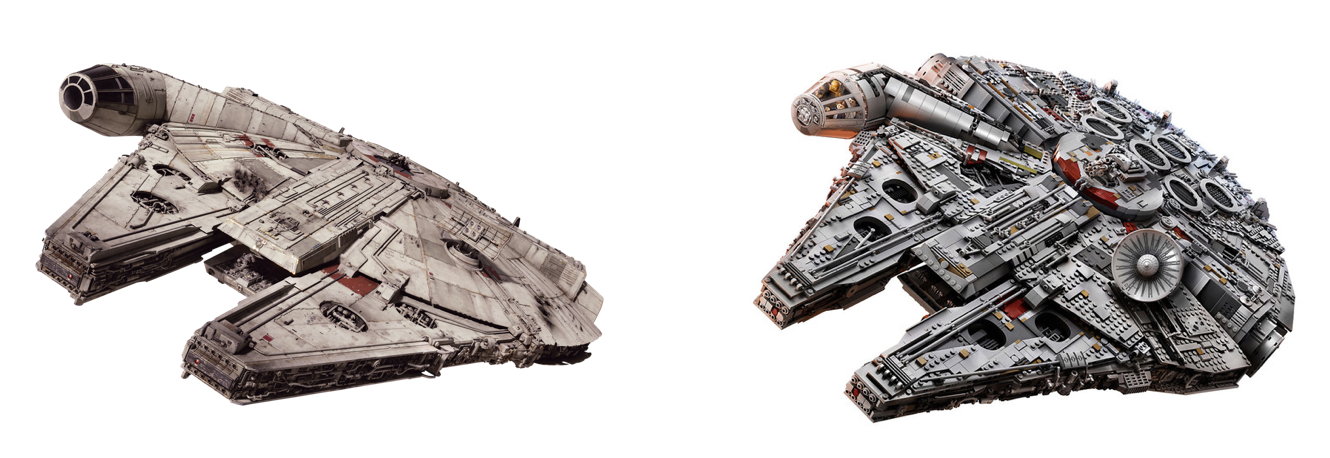
\includegraphics[width=\textwidth]{figures/MillenniumFalcon.png}
\end{figure}
These ingredients come together through a tool called a Feynman diagram.

\section{Diagrammar}

Fig.~\ref{fig:ee:gamma:gamma:example} is an example of a Feynman diagram.
\begin{marginfigure}%[th]
    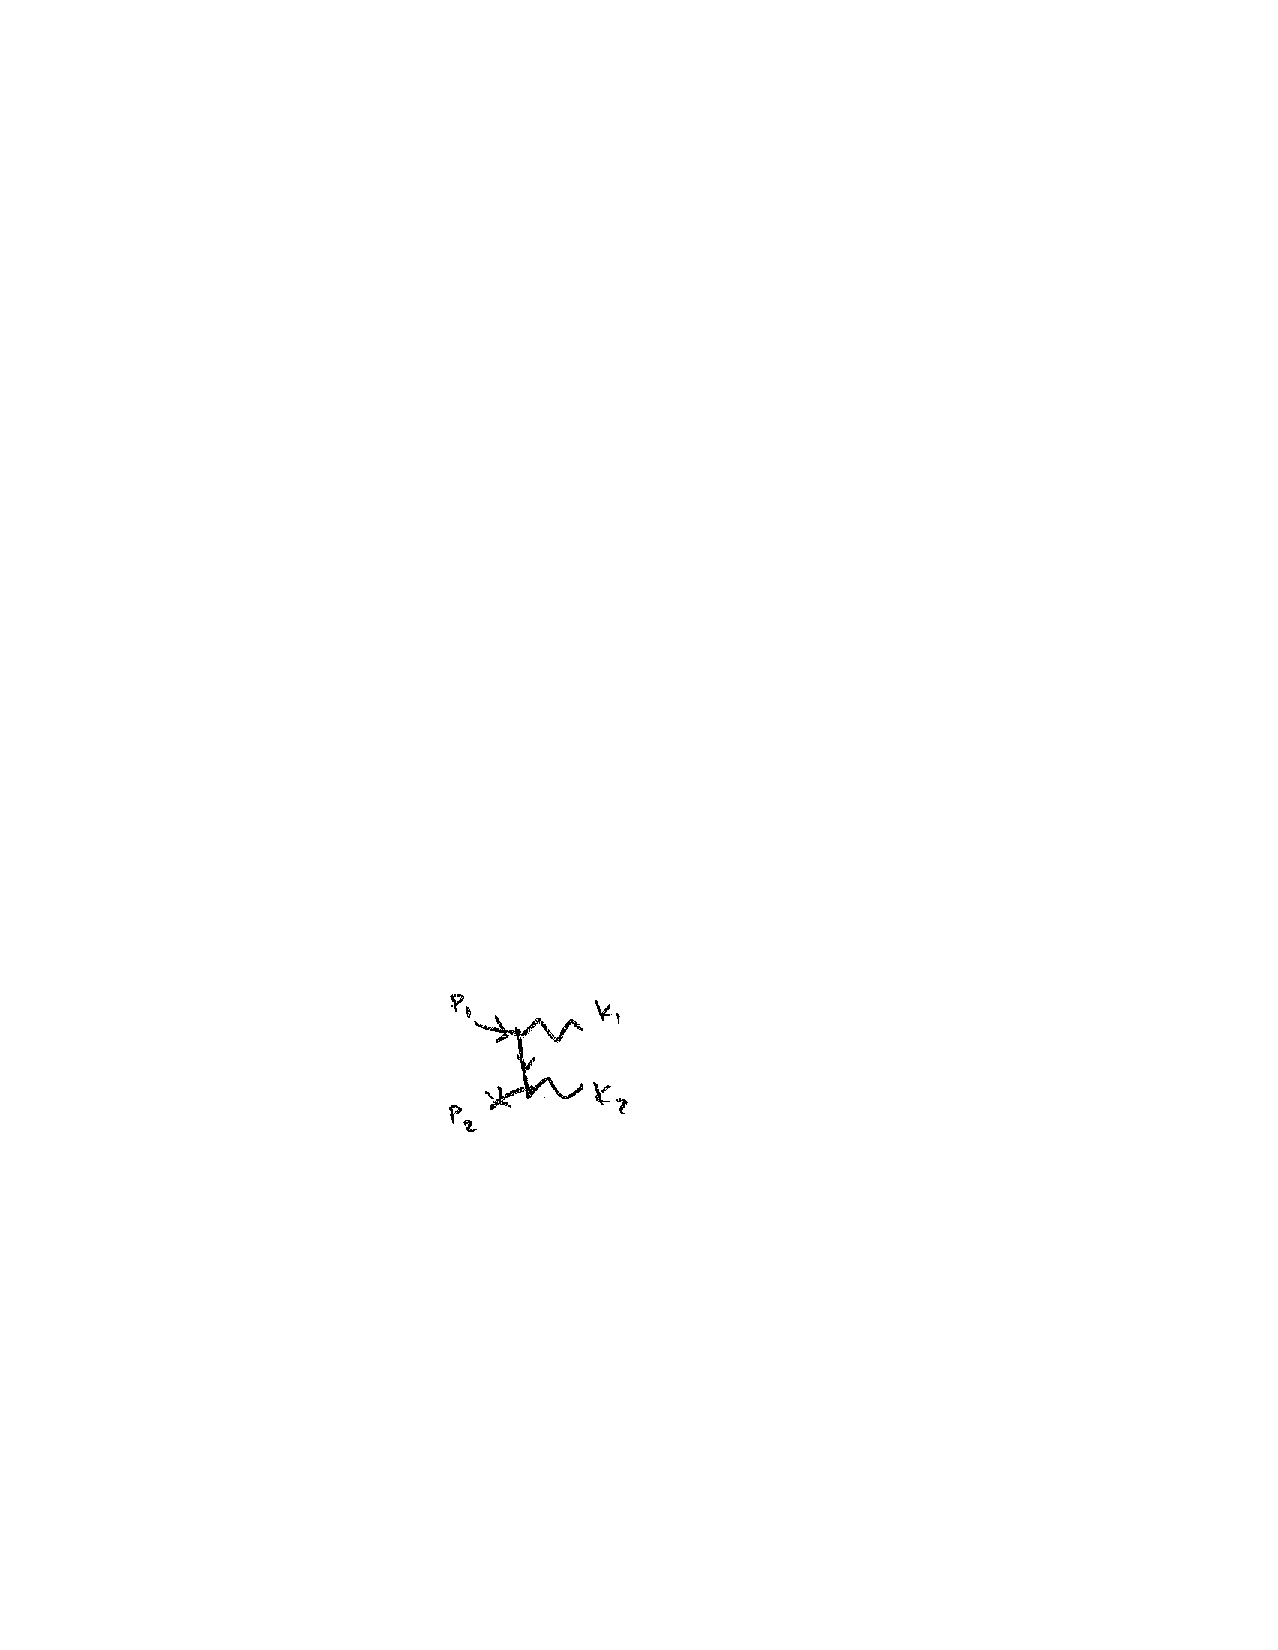
\includegraphics[width=.8\textwidth]{figures/feyn_eegaga.pdf}
    \captionsetup{font={scriptsize,sf}}
    \caption{Example of a Feynman diagram. Here an electron and a positron annihilate into a pair of photons.}
    \label{fig:ee:gamma:gamma:example}
\end{marginfigure}
Feynman diagrams are a perturbative expansion of the quantum mechanical amplitude for a something to happen. You may recall that the quantum amplitude is a ``square root of the probability\footnote{This notion comes from quantum mechanics where the probability of observing a state $\ket{\Psi}$ is $\langle \Psi | \Psi\rangle = |\Psi|^2$. In quantum field theory we typically talk about \emph{cross sections}, $\sigma$. The relation between the amplitude $\mathcal M$ and cross section is $\sigma \sim |\mathcal M|^2$ and contains kinematic factors. We determine these kinematic factors in subsequent chapters.}.'' The statement that diagrams are a \emph{perturbative expansion} means that there is some small parameter for which we are performing a Taylor expansion\sidenote{Formally the amplitudes are complex and may contain singularities. It is thus more appropriate to say that this is a \emph{Laurent expansion}. One of the `deep' ideas in quantum field theory is the intimate relationship of \emph{analyticity} (complex differentiability) to physical properties. To dig deeper, see my Physics 231 notes.\footnotemark}\footnotetext{\url{https://sites.google.com/ucr.edu/p231/}}. In the standard case, this perturbative expansion is usually an expansion in couplings.

By \textbf{coupling} I mean a parameter of the theory that determines how much some particles interact with each other. When the coupling is large, the interaction is very strong. When the coupling is small, the interaction is very weak. One coupling that you may be familiar with is the electrodynamic coupling, $e$. You are probably most familiar seeing $e$ as an ingredient in the fine structure constant, 
\begin{align}
    \alpha = \frac{1}{\hbar c \varepsilon_0} \frac{e^2}{4\pi} \approx \frac{1}{137} \ .
\end{align}
The first factor of $(\hbar c \varepsilon_0)^{-1}$ are relics of using silly units. When we use natural units---see Sec.~\ref{sec:units:dimensions}---these are set to one. You can see that $1/137$ is a small number, so it at least makes sense that if we had some amplitude $\mathcal M(\alpha)$ that is a function of the electrodynamic couplings through $\alpha$ that we could imagine doing the perturbative expansion
\begin{align}
    \mathcal M = \mathcal M_0 + \alpha \mathcal M_1  + \alpha^2 \mathcal M_2 + \cdots \ ,
    \label{eq:amplitude:perturbative:expansion}
\end{align}
and then dropping any subleading terms since we expect them to be percent-level corrections. If the couplings are large, then this expansion breaks down because subsequent terms are not small. In fact, this is what happens with the strong interactions (quantum chromodynamics), the force that holds nuclei together. Thus there are regimes where the usual Feynman expansion fails: it seems like we should not use these diagrams to describe the interactions of the quarks and gluons that are `inside' a proton.
\begin{example}
I seem to have implied that Feynman diagrams do not work for the strong interaction. Despite this, collider physicists working on the Large Hadron Collider `speak' the language of Feynman diagrams. They'll even draw diagrams that involve the strong force. What gives? Apparently I haven't told you the whole story...
\end{example}
Note that I wrote \emph{couplings} not the common phrase \emph{coupling constants}. That is because---brace yourselves---these couplings are generally \emph{not} constant. In fact, they depend on the energy scale at which you probe them. If I smash together color-charged particles\sidenote[][]{In this class and in this field, we write \emph{colored} to mean color-charged, or charged with respect to the strong force. See Chapter~5 of \emph{The Disordered Cosmos} for an anthropological discussion.\footnotemark}\footnotetext{\cite{prescod2021disordered}} at high energies, the analogous fine structure parameter for the strong force, $\alpha_\textnormal{s} = g_\textnormal{s}^2/4\pi$ depends on the characteristic energy scale\footnote{We write $\sqrt{Q^2}$ rather than $E$ because $Q^2$ is a Lorentz-invariant quantity, as we explain below in our review of special relativity.} $\sqrt{Q^2}$ at which one probes the interaction, see Fig.~\ref{fig:aS:running:from:1604.08082}. 
\begin{marginfigure}%[th]
    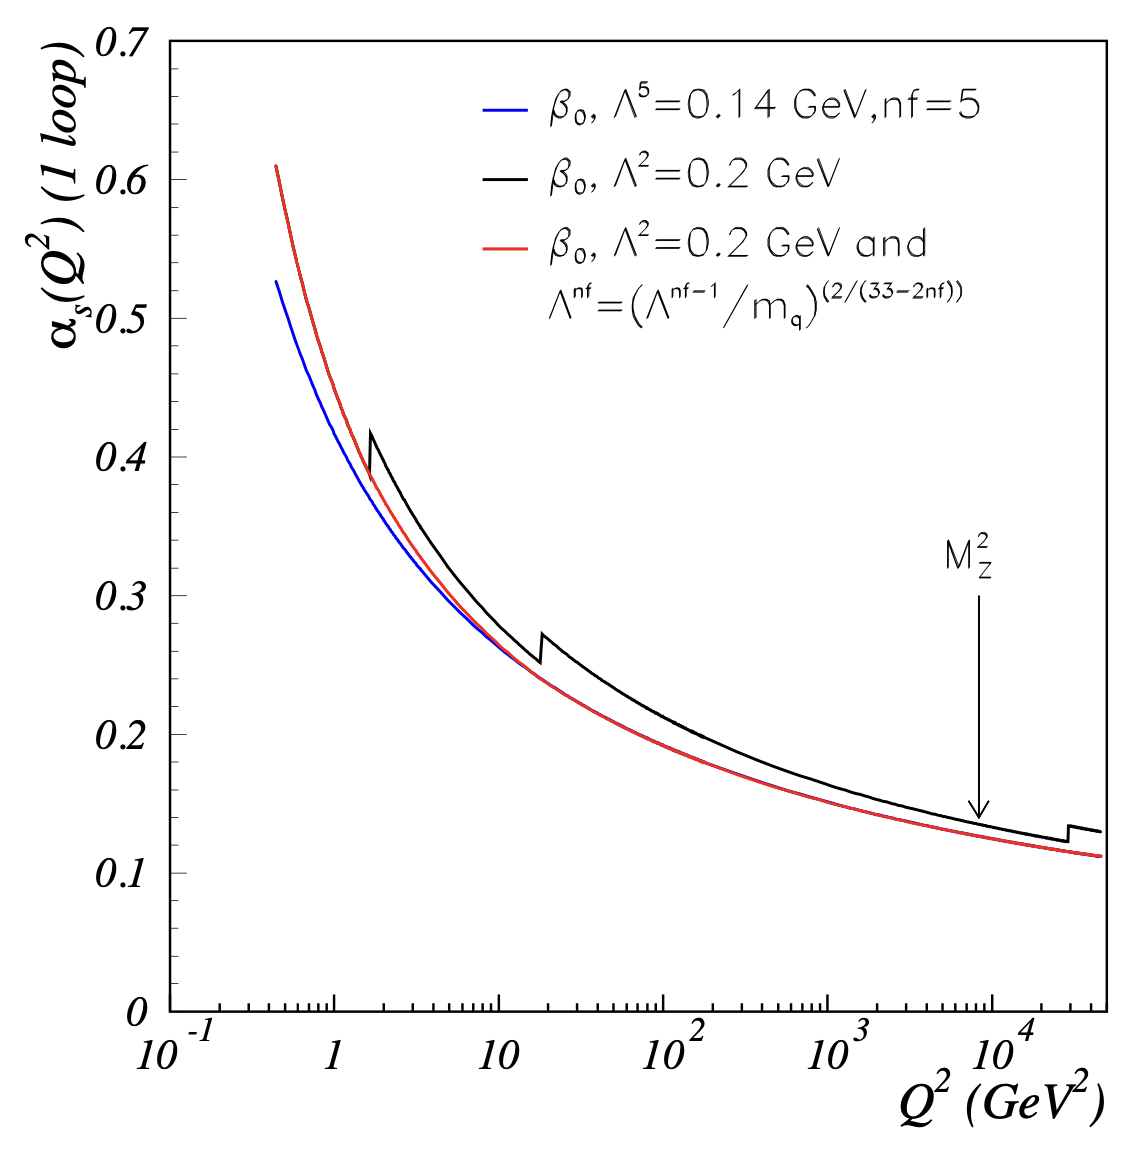
\includegraphics[width=.8\textwidth]{figures/aSrun_1604.08082.png}
    \captionsetup{font={scriptsize,sf}}
    \caption{Approximate value of the strong force fine structure parameter, $\alpha_\textnormal{s}$. Lines correspond to slightly different calculations. The horizontal axis is the square of the characteristic energy scale at which $\alpha_\textnormal{s}$ is being measured. From Fig.~3.2 of \arXiv{1604.08082}.}
    \label{fig:aS:running:from:1604.08082}
\end{marginfigure}
This idea should be shocking the first time that you see it. The `coupling constants' are not constant at all. The meaning of this oddity is an idea called \emph{renormalization} and is rooted in making sense of what the \emph{actual} small parameter is in perturbation theory: it turns out not to be the fine structure constant, but the fine structure constant times a function of the kinematics of a process. This means that at sufficiently high energies, we can meaningfully talk about Feynman diagrams of quarks exchanging gluons. However, at low energies, these diagrams lose their meaning. If you were paying attention in the previous sub-section, this is the regime where particle physics becomes nuclear physics.
\begin{example}
This reminds me of the difference between a \emph{physicist} and a \emph{physics fan}. A physics fan is someone who thinks that $1/137$ is a fundamental constant of the universe and so should be tattooed on their body. A physicist stops to think: \emph{Where does this number come from?} and proceeds to learn about the scale-dependence of the electric coupling. In fact, in this course you will find that the electric coupling is not even a fundamental parameter but a combination of more fundamental parameters. I do not care whether or not you are a physics fan, but my goal is to train you as a physicist.
\end{example}

\begin{exercise}
On the subject of couplings: is the gravitational coupling \emph{large} or \emph{small} relative to the electromagnetic coupling? You may recall from popular physics that one of these is [surprisingly?] much stronger than the other. Try to make this quantitative by comparing two numbers. \textsc{Hint}: this is a bit of a trick question. Try writing out the gravitational fine structure constant and argue why it appears that you cannot meaningfully compare it to the electromagnetic coupling.
\end{exercise}

Feynman diagrams are graphs that represent a mathematical expression for a complex number. The graphs are trajectories in spacetime that we read from left to right. Each line in a diagram represents a particle. The lines may have decorations or labels that indicate their identity. In Fig.~\ref{fig:ee:gamma:gamma:example} the two lines on the left are an electron and a positron. The two wiggly lines on the right are each photons. Each vertex (intersection of lines) represents a factor of the coupling. In Fig.~\ref{fig:ee:gamma:gamma:example} the two vertices mean that this diagram contains two powers of the electric coupling, $e$. Thus this diagram contributes to the $\mathcal O(e^2) = \mathcal O(\alpha)$ term in the expansion of the amplitude $\mathcal M(e^+e^-\to \gamma\gamma)$ in \eqref{eq:amplitude:perturbative:expansion}. The notation $\mathcal M(e^+e^-\to \gamma\gamma)$ simply means the amplitude for an electron $e^-$ and a positron $e^+$ to turn into two photons, $\gamma\gamma$.

Something else that may be familiar from quantum mechanics: amplitudes sum together. This is the origin of quantum interference and all of the fun parts of quantum physics. Our perturbative expansion \eqref{eq:amplitude:perturbative:expansion} is one example of such a sum. However there are usually multiple diagrams that contribute at a given order in perturbation theory. One of the brilliant things about these diagrams is that they have a complementary interpretation: as a \emph{sum over histories}. This is an idea that we emphasize in our review of quantum mechanics, but the idea is this: 
\begin{quote}
The amplitude to go from some initial state to some final state is represented by the sum of all Feynman diagrams that connect the initial state to the final state. Each individual Feynman diagram in the sum represents a possible history that the initial state could have taken to reach the final state.
\end{quote}
This sum over histories interpretation is outrageous the first time you see it but is ultimately an extension of the principle of least time that underlies Snell's law in optics. The generalization to a principle of least action is the core of Lagrangian mechanics and was in fact Feynman's Ph.D thesis\autocite{feynman2005feynman}. 

The diagrams are simply a tool. Feynman's long time physics rival and co-Nobel prize winner, Julian Schwinger, was a master of calculating amplitudes in quantum field theory \emph{without} any diagrams. In one interpretation of history, Feynman's main contribution at this stage of physics history was bringing that calculational technology to the masses by giving each term an intuitive meaning.\sidenote{It is no surprise that he is also (mis-)attributed as the spokesperson of the ``shut up and calculate'' school of quantum physics.\footnotemark}\footnotetext{\cite{10.1063/1.1768652}} Veltman has a nice physics-oriented history of the spread of Feynman diagrams in his book \emph{Diagrammatica}\autocite{Veltman:1994wz}. This book should not be confused with a set of lecture notes he co-wrote with 
't~Hooft called ``Diagrammar\autocite{tHooft:1973wag},'' which inspired the name of this section.
% Not for this class, but also interesting: https://arxiv.org/abs/2109.06889
% Diagrammar of physical and fake particles and spectral optical theorem
%  Anselmi


As a final note: there is far more to quantum field theory than Feynman diagrams. As a perturbative expansion, Feynman diagrams represent the \emph{easiest} part of quantum field theory. But just as there are functions that cannot be meaningfully Taylor expanded\sidenote{Try expanding $\exp(-x^{-2})$ around the point $x_0 = 0$. Every term at every order vanishes, even though the function is well defined and non-zero away from the origin. The quantum field theory analog is something called an instanton and is beyond the scope of this course.}, there are vast swaths of field theory that are intrinsically \emph{non-perturbative}. Quantum chromodynamics at low energies---where we must turn to methods in nuclear physics---is one example. We make this caveat to emphasize that although we lean heavily on the diagrammatic interpretation of particle physics, we are still just scratching the surface.



% HW: muon shot. 
% Idea: every homework is a story



\section{Kinematics and Dynamics}

I may be the only person who makes a big deal about this, but we can separate our study of particle physics into two parallel tracks: {kinematics} and {dynamics}. You probably know that these words ``have to do with physics,'' but the distinction between them is rarely delineated. In fact, I suspect I may be making it up---in which case, here are the working definitions for this class. 

\textbf{Kinematics}\index{kinematics} has to do with the motion of particles through space and time. The kinematics of a scattering process relates to the momentum and energy of those particles. The conservation of energy and momentum are also kinematical facts\sidenote{Though their derivation through Noether's theorem is arguably a statement about dynamics.}. The thread of physics that is most relevant to this study is \emph{relativity}, and in particular the flat-spacetime version known as \emph{special relativity}.\sidenote{In contrast, general relativity is the study non-flat spacetimes. One can argue that it is the \emph{dynamics} of spacetime itself.}

\textbf{Dynamics}\index{dynamics}, on the other hand, has to do with the rules for how particles interact. When we talk about a theory or a model of particle physics, we usually mean a description of the dynamics. These are encoded in the action or Lagrangian of a theory. The dynamics of a theory draws primarily from the rules of \emph{quantum mechanics}.

Feynman diagrams are an output of the dynamics of a theory. However, a Feynman diagram is only physically meaningful if it obeys the rules of the kinematics of a theory. Kinematics are an additional consideration when we convert the squared amplitude into something physically measurable.
\begin{example}
You can draw a Feynman diagram for a process like $\gamma \to e^+e^-$ by which a photon decays into an electron--positron pair. You could even calculate the amplitude for this process to happen. However, this process is kinematically forbidden because it cannot simultaneously conserve energy and momentum. The amplitude is nonzero, but the decay rate is forced to be zero by kinematics.
\end{example}
\begin{exercise}
Show that both energy and momentum cannot be conserved in $\gamma \to e^+e^-$. There are many ways to do this, including some that are more slick than others. If you are stuck, come back to this exercise after our review of special relativity.
\end{exercise}

In this course, you can think of dynamics as the set of rules\sidenote{Called \emph{Feynman rules}.} that tell us how we may construct Feynman diagrams. These rules are an encoding of the Lagrangian of the theory.  You can think of kinematics as conditions on the energies and momenta of the initial and final states of an amplitude---these are the external lines of a diagram. Notably, kinematic constraints do not apply to the particles on the \emph{inside} of a Feynman diagram. Lines that obey the kinematic constraints are called \textbf{on shell}, while those that do not are called \textbf{off shell}.\sidenote{What is the \emph{shell}? It is the hypersurface the four-dimensional space of energy and momentum that satisfies the Einstein relation, $E^2 = m^2c^4 + p^2 c^2$ for a particle of mass $m$, energy $E$, and three-momentum $p$.} With this jargon, we say that external lines on a Feynman diagram represent parts of the initial or final states of a process and must be on shell. Internal lines are, in general, off shell.

\subsection{Symmetry}

The notion of \emph{symmetry} plays a central role for both the kinematics and the dynamics. The mathematical description of symmetry is called group theory and the way in which symmetries act on objects is called representation theory.\sidenote{I am name-dropping subjects because I am often asked what subjects should an aspiring theoretical physicist master.} The tables of Clebsch--Gordan coefficients that you may have invoked in your study of addition of angular momentum in quantum mechanics is an output of the representation theory of the group of three-dimensional rotations. In this course we are specifically interested in the representation theory of continuous groups---symmetries like rotations where you can transform by an arbitrary amount---called \emph{Lie groups}.\sidenote{Pronounced `lee.'} As humble physicists\sidenote{Oppenheimer: Well, if that’s how you treat a lieutenant colonel than I hate to see how you treat a humble physicist.\\Leslie Groves: If I ever meet one I'll let you know. (From \emph{Oppenheimer}, 2023)} the way we work with symmetries is to introduce indices. Objects that carry these indices are called \textbf{tensors}.

In special relativity (kinematics) the simplest tensors are four-vectors. They are called four-vectors because they are vectors that have four components. For example, the four-momentum of a particle may be written $p^\mu$. The index is $\mu$. There is a related object called $p_\mu$ with a lower index. These are related by a tensor called the metric tensor, which for our purposes we write $\eta_{\mu\nu}$. The metric gives us a way to define an inner product. This should all sound familiar from linear algebra because this \emph{is} linear algebra. In representation theory, the objects that get rotated\sidenote{By `rotate' I mean a general symmetry transformation. For the case of special relativity, one can have boosts in addition to rotations.} are vectors in a vector space. If you ever wonder why I teach Physics 17 the way that I do, it is because I want students to be primed to understand representation theory as it appears in physics.

Maybe the phrase `inner product' caught your ear. This is the same idea that comes up in quantum mechanics. In fact, now you may recall that quantum mechanics really boils down to complex linear algebra. In fact, many ideas in quantum mechanics are ultimately group theoretical. For example, the commutator is the natural multiplication operation between elements of a group.\sidenote{Check that while this may be surprising, it is sensible. The commutator of two operators is another operator in the same way that the multiplication of two things of a given type should be another thing of the same type.} Furthermore, finite transformations are the exponentiation of infinitesimal transformations. For example, the Hamiltonian $\hat H$ is the generator of translations in time. A finite translation in time is
\begin{align}
    \hat U(t) = e^{-i \hbar t\hat H} \ .
    \label{eq:Ut:time:H}
\end{align}
\flip{check the $\hbar$}
In particle physics we will meet several \textbf{internal symmetries} that mathematically describe the rotation of an object in different vector spaces. These do \emph{not} correspond to spacetime rotations or boosts. Instead, they may represent a rotation between quarks of different color charges.\sidenote{We define these carefully below where we discuss quantum chromodynamics. For this introduction just humor me and go with the flow to appreciate the big idea.} The infinitesimal generators of these transformations take the form\footnote{I am using `physicist' shorthand here and referring to a tensor by its components. Supercilious mathematicians sneer at us for this. Formally, $A\aij{i}{j}$ is not a matrix, it is the $i$--$j$ \emph{component} of a matrix A. Physicists justify our sloppiness because anyone who is paying attention should understand what we mean and, more importantly, by keeping the indices explicit we can see how the tensor transforms.}
\begin{align}
(T^A)\aij{i}{j}\ ,    
\end{align}
where we recognize three indices. The index $A$ is called an adjoint index and tells you which direction you are rotating. For the rotation group, $A$ takes values from 1 to 3 corresponding to rotations about the $x$, $y$, and $z$ axes. All other rotations are combinations of these. The other two indices, $i$ and $j$ depend on the \emph{representation} of the object that we are rotating. 
\begin{example}
In quantum chromodynamics we there are eight generators of so-called color symmetry. This means $A$ takes values from 1 through 8. This group is called \acro{SU(3)}, which stands for the set of $3\times 3$ special unitary matrices.\sidenotemark A quark has indices that I conventionally write with lowercase letters from the middle of the Roman alphabet that take values $m$ from 1 to 3 corresponding to red, blue, and green. The matrix $(T^4)\aij{m}{n}$ represents a particular rotation around the $A=4$ axis. A finite transformation by angle $\theta$ takes the form 
\begin{align}
    q^m \to \sum_n e^{i \theta (T^4)\aij{m}{n} } q^n \equiv \sum_n U(\theta)\aij{m}{n}q^n \ ,
\end{align}
where the sum over $n$ is what we expect from matrix multiplication.
\end{example}\sidenotetext[][]{Special means unit determinant. Unitary, as you may recall from quantum mechanics, means that the hermitian conjugate is its inverse.}

This is all to say that indices feature front-and-center in this course. They are a crutch for us to talk about the underlying symmetries that govern both the kinematics and dynamics of particle physics. We will spend a good chunk of this course building familiarity with how to interpret and manipulate indices. This is a mathematical skill that is far more general than particle physics itself.





\section{Natural Units}
\label{sec:units:dimensions}

By this stage of your physics career you are an expert at converting units. The trick is to multiply be one in different forms. Suppose you have some unit $x$ that is related to unit $y$ by some prefactor,
\begin{align}
    x = a y \ . \label{eq:unit:conversion}
\end{align}
Then you can derive that
\begin{align}
    1 = \frac{ay}{x} = {x}{ay} \ .
    \label{eq:multiply:by:one:unit:conversion}
\end{align}
Then if some quantity is, say, $3.4\,x$, you know that you can write it out in terms of $y$ simply by multiplying by one, cleverly written:
\begin{align}
    3.4\,x = 3.4\times 1 \times x = 3.1 \times \frac{ay}{\cancel{x}} \times \cancel{x}
    = (3.4a)\, y \ .
\end{align}
\eqref{eq:multiply:by:one:unit:conversion} tells us that there is a universal, unambiguous constant ratio that relates unit $x$ to unit $y$. 


\begin{example}
Suppose someone tells you the number of feet in a mile,
\begin{align}
    1~\text{mile} = 5280~\text{feet} \ .
\end{align}
This number just so happens to be the mass of the $B$ meson in \acro{MeV}.
You can derive that
\begin{align}
    1 = 5280~\frac{\text{feet}}{\text{mile}}
    = \frac{1}{5280}~\frac{\text{mile}}{\text{feet}} \ .
\end{align}
From this you can deduce that a distance of $1.5$ miles is
\begin{align}
    1.5\,\text{mile} = 
    1.5\,\cancel{\text{mile}} \times \left(5280~\frac{\text{feet}}{\cancel{\text{mile}}}\right) = 
    7920~\text{feet} 
    \approx 8000~\text{feet} 
    \ .
\end{align}
\end{example}

If this all looks completely simple then \emph{good}, it is supposed to. There is nothing deep or mysterious about changing units. Let us really put it to work. \textbf{Natural units}\index{natural units} are a convenient choice that boils down to the following identifications:
\begin{align}
    c &=1  &
    \hbar &= 1
    \ .
\end{align}
That's right. The speed of light $c$ and reduced Planck's constant $\hbar$ are set to one. This may bother you. After all, you know from past coursework that these are \emph{not} dimensionless quantities:
\begin{align}
    c &= 3\times 10^{8}\,\frac{\textnormal{m}}{\textnormal{s}}
    &
    \hbar &= 1\times 10^{-34}\,\frac{\textnormal{m}^2 \textnormal{kg}}{\textnormal{s}} \ .
    \label{eq:c:hbar:SI}
\end{align}
Setting $c = 1$ would then mean that there is an unambiguous way conversion between length and time, as if these were measuring the ``same thing.'' But length is measured by rulers and time is measured by clocks: how are these the same? They are the same \emph{precisely} because nature\sidenote{All our observations since the Michelson--Morley experiment are consistent with a constant speed of light and this is built into our theory of special relativity. Theoretically this is an aesthetic unification of space and time that laid the foundation of general relativity, which in turn has passed every experimental prediction.} gives us a universal, unambiguous constant ratio that relates units of length into units of time. This constant is the speed of light.
\begin{example}
A lightyear is a unit of distance. It is defined to be the distance traversed by a particle traveling at the speed of light,
\begin{align}
    \text{lightyear} = c\, \text{year} \ ,
\end{align}
where we see that the speed of light in natural units $c=1$ plays the role of a conversion factor in \eqref{eq:unit:conversion}. 
\end{example}
% Naive dimensional analysis
% \autocite{Manohar:1983md,Georgi:1986kr,Georgi:1992dw}
Identifying the speed of light as a conversion factor ends up relating another set of dimensionful quantities. All velocities in natural units are dimensionless. This is because we can simply write any velocity in units of the speed of light.
\begin{example}
The tangential speed of the Earth around the solar system is around $v = 200$\,km/s. In natural units this is a dimensionless number:
\begin{align}
v = 200\,\frac{ \textnormal{km} }{ \textnormal{s} }
=
2\times 10^{5} \, \frac{\textnormal{m}}{\textnormal{s}} 
\times 
\left(\frac{1}{3\times 10^8}\frac{\textnormal{s}}{\textnormal{m}}\right)
= 7 \times 10^{-3} \ .
\end{align}
In natural units, any sensible velocity has magnitude less than one. Otherwise something is traveling faster than the speed of light. 
\end{example}
\begin{exercise}
What goes wrong in physics if a particle can travel faster than the speed of light? \textsc{Hint}: review the relativity of simultaneity. 
\end{exercise}
Velocities are dimensionless in natural units. 
Recall that energy has the units of mass times velocity squared. You may recall this from from 
\begin{align}
    E_\textnormal{kinetic} = \frac{1}{2} mv^2 \ .
\end{align}
You may argue that this formula is only true for kinetic energy. That is true, energy---no matter what the form---is carries the same type of dimension. Because velocities are dimensionless, then the dimensions of energy and the dimensions of mass must be the same. In other words, mass and energy are ``the same thing.'' Given a particle of some mass---say the mass of a proton, $m_\textnormal{p}$---there is an associated energy that is $m_\textnormal{p} \times 1  = m_\textnormal{p} c^2$. This looks remarkably like the non-relativistic limit of the Einstein relation,
\begin{align}
    E = mc^2 \ .
\end{align}
Indeed, in that limit, the Einstein relation just tells us that mass and energy are the same thing. The square of the speed of light plays the role of a conversion factor between them. It is conventional for particle physicists using natural units to measure everything in units of energy. A particularly useful energy scale is 
\begin{align}
    m_\textnormal{p} = 1\,\text{\GeV{}} \ .
\end{align}
To one significant figure, the mass of the proton happens to be about one billion times an electron volt.  
\begin{exercise}
How much do you weigh in \GeV{}? 
\end{exercise}
Sometimes we lapse into other powers of electron volt. Some useful values are the mass of the electron and the mass of the Higgs boson\sidenote{We write $m_h$ to three significant figures because the Higgs is a big deal.}, and the center-of-mass energy of proton-proton collisions at the Large Hadron Collider:
\begin{align}
    m_e &= 0.5\,\text{MeV}
    &
    m_h &= 125\,\text{GeV}
    &
    E_\text{cm} &= 14\,\text{TeV} \ .
\end{align}



What about $\hbar = 1$? Planck's constant carries units of angular momentum\sidenote{These are also the units of action, $S=\int dt\,L$.}, or energy times time. Using the just-established equivalence of mass and energy in natural units, this tells us that
\begin{align}
    \hbar &= 7 \times 10^{-22}\,\textnormal{MeV}\,\textnormal{s}  \equiv 1 \ . 
\end{align}
% \begin{align}
%     \hbar = 10^{-34}\,\frac{\textnormal{m}^2 \textnormal{kg}}{\textnormal{s}}
%     \times 
%     \left(3\times 10^{8}\,\frac{\textnormal{m}}{\textnormal{s}}\right)^{-2}
%     = 
%     10^{-51}\,\textnormal{kg}\,\textnormal{s} \ .
% \end{align}
This means that the fundamental unit of ``quantum-ness'' tells us that time and inverse energy are ``the same thing.''
\begin{example}
How would you measure $\hbar$ to determine that it is a universal constant? Like measuring $c$, there are many options. You could look at the deflection of particles in a Stern--Gerlach experiment, measure distributions of position uncertainties given multiple measurements of a momentum eigenstate, the spectrum of hydrogen (and corrections thereof), etc. 
\end{example}
At this point, you can multiply and divide by $c$ and $\hbar$ as needed to write all dimensionful parameters in units of \GeV{} to some power. 
\begin{example}
An additional conversion is to set the Boltzmann factor, $k_\textnormal{B} =1$. This is the observation that thermal energy is energy and can be measured in \GeV{}.
\end{example}
We provide a useful table for conversions to one significant figure.
\begin{table}[ht]
    \renewcommand{\arraystretch}{1.3} % spacing between rows
    \centering
    \sidecaption[Useful conversions to natural units. Adapted from Palash Pal's website.][-2\baselineskip]{%
        Conversion of units using $\hbar = c = k_\textnormal{B} = 1$. The row heading is equal to the table entry times the column heading so that a \GeV{} is a small number of Planck masses, $M_\textnormal{Pl}$.  Adapted from Palash Pal's website.\footnotemark 
  %       \label{table:app:natural:unit:conversion}
    }
    \begin{tabular}{ @{} lllllll @{} } \toprule % @{} removes space
        & \GeV{} & g & K & cm$^{-1}$ & sec$^{-1}$ & M$_\textnormal{Pl}$
        \\ \midrule
        \GeV{} % col
        & % GeV
        & 1$\times 10^{-24}$ % g
        & 1$\times 10^{13}$% K
        & 5$\times 10^{13}$% cm-1
        & 2$\times 10^{24}$% s-1
        & 8$\times 10^{-20}$% Mpl
        \\
        g % col
        & 6$\times 10^{23}$% GeV
        & %$\times 10^{}$% g
        & 7$\times 10^{36}$% K
        & 3$\times 10^{37}$% cm-1
        & 9$\times 10^{47}$% s-1
        & 5$\times 10^{4}$% Mpl
        \\
        K% col
        & 9$\times 10^{-14}$% GeV
        & 2$\times 10^{-37}$% g
        & %$\times 10^{}$% K
        & 4%$\times 10^{}$% cm-1
        & 1$\times 10^{11}$% s-1
        & 7$\times 10^{-33}$% Mpl
        \\
        cm$^{-1}$ % col
        & 2$\times 10^{-14}$% GeV
        & 4$\times 10^{-38}$% g
        & 2$\times 10^{-1}$% K
        & %$\times 10^{}$% cm-1
        & 3$\times 10^{10}$% s-1
        & 2$\times 10^{-33}$% Mpl
        \\
        sec$^{-1}$ % col
        & 7$\times 10^{-25}$% GeV
        & 1$\times 10^{-48}$% g
        & 8$\times 10^{-12}$% K
        & 3$\times 10^{-11}$% cm-1
        & %\times 10^{}$% s-1
        & 5$\times 10^{-44}$% Mpl
        \\
        M$_\textnormal{Pl}$% col
        & 1$\times 10^{19}$% GeV
        & 2$\times 10^{-5}$% g
        & 1$\times 10^{32}$% K
        & 6$\times 10^{32}$% cm-1
        & 2$\times 10^{43}$% s-1
        & %$\times 10^{}$% Mpl
        \\ \bottomrule
    \end{tabular}
  %   \caption[Useful conversions to natural units. Adapted from Palash Pal's website.]
  %   {
  %       Conversion of units using $\hbar = c = k_\textnormal{B} = 1$. The row heading is equal to the table entry times the column heading so that a \GeV{} is a small number of Planck masses, $M_\textnormal{Pl}$.  Adapted from Palash Pal's website.\footnotemark 
        \label{table:app:natural:unit:conversion}
  % }
\end{table}\footnotetext{\url{https://www.saha.ac.in/theory/palashbaran.pal/conv.html}}

\begin{example}[Mnemonics]
You can use your favorite equations in physics as mnemonics for natural units. We already saw how $E=mc^2$ reminds us that energy and mass both carry the same units. You can also invoke Heiseinberg's uncertainty relations
\begin{align}
    \Delta x\,\Delta p &\sim \hbar 
    &
    \Delta E \Delta t &\sim \hbar
\end{align}
to remind us that momentum and distance carry reciprocal units, as do energy and time. Because $c=1$ tells us that distance and time are the same, we find
\begin{align}
    \text{length} \sim \text{time} \sim \frac{1}{\text{mass}} 
    \sim \frac{1}{\text{energy}} \ .
\end{align}
\end{example}

The great thing about natural units is that we just have to keep track of one unit, say \GeV{}. Dimensional analysis is very simple and we introduce the bracket notation:
\begin{align}
    [x] \defeq ``\text{dimensions of }x \ .''
\end{align}
$[x]$ means: what power of energy is the unit of quantity $x$?
\begin{example}
For a distance $\ell$, time $t$, mass $m$, and energy $E$:
\begin{align}
    [\ell] &= -1
    &
    [t] &= -1
    &
    [m] &= 1
    &
    [E] &= 1
    \ .
\end{align}
\end{example}
\begin{exercise}
What are the dimensions of the gravitational constant, $[G_\textnormal{N}]$? \textsc{Hint}: you can use the force law for gravity to figure out the \acro{SI} units of $G_\textnormal{N}$.
\end{exercise}

\begin{exercise}
Show that the units of action are the same as the units of angular momentum. \textsc{Hint}: use the expression for the action with your favorite choice of Lagrangian.
\end{exercise}

\begin{example}[Collider physics as microscopy]
The Large Hadron Collider is a microscope. The center of mass energy of the proton--proton collisions is $E = 10~\textnormal{TeV}$. To convert this into a length scale, we divide by \ .
\begin{align}
    \hbar c = 10^{21}\frac{1}{\textnormal{MeV}\,\textnormal{s}} \times 10^{-8} \frac{\textnormal{s}}{\textnormal{m}}
\end{align}
This gives us
\begin{align}
    E &= 10^7~\textnormal{MeV} \times 10^{21}\frac{1}{\textnormal{MeV}\,\textnormal{s}} \times 10^{-8} \frac{\textnormal{s}}{\textnormal{m}}
    \\
    &= \frac{1}{10^{-20}\,\textnormal{m}} \ .
\end{align}
The length scale associated with $10~\textnormal{TeV}$ is tiny: $10^{-20}~\textnormal{m}$. Compare this to the typical atomic length, $\text{\AA} = 0.1~\textnormal{nm} = 10^{-10}~\textnormal{m}$. The inverse relation $\ell \sim E^{-1}$ makes it clear that increasing the energy decreases the length scale. 
\end{example}

We can understand the $E \sim \ell^{-1}$ relation from ordinary optical microscopy. As we increase the energy of a photon, we increase its frequency and therefore decrease its wavelength, $\lambda$. We need the wavelength of the probe to be \emph{smaller} that the characteristic size features that we are studying, $\lambda \ll \Delta x$. Figure~\ref{fig:subfig:waves} demonstrates this idea by showing rocks of different sizes in a stream with water waves of uniform scale $\lambda$.

\begin{figure}%[th]
    \centering
    \begin{subfigure}{0.3\textwidth}
    \centering
        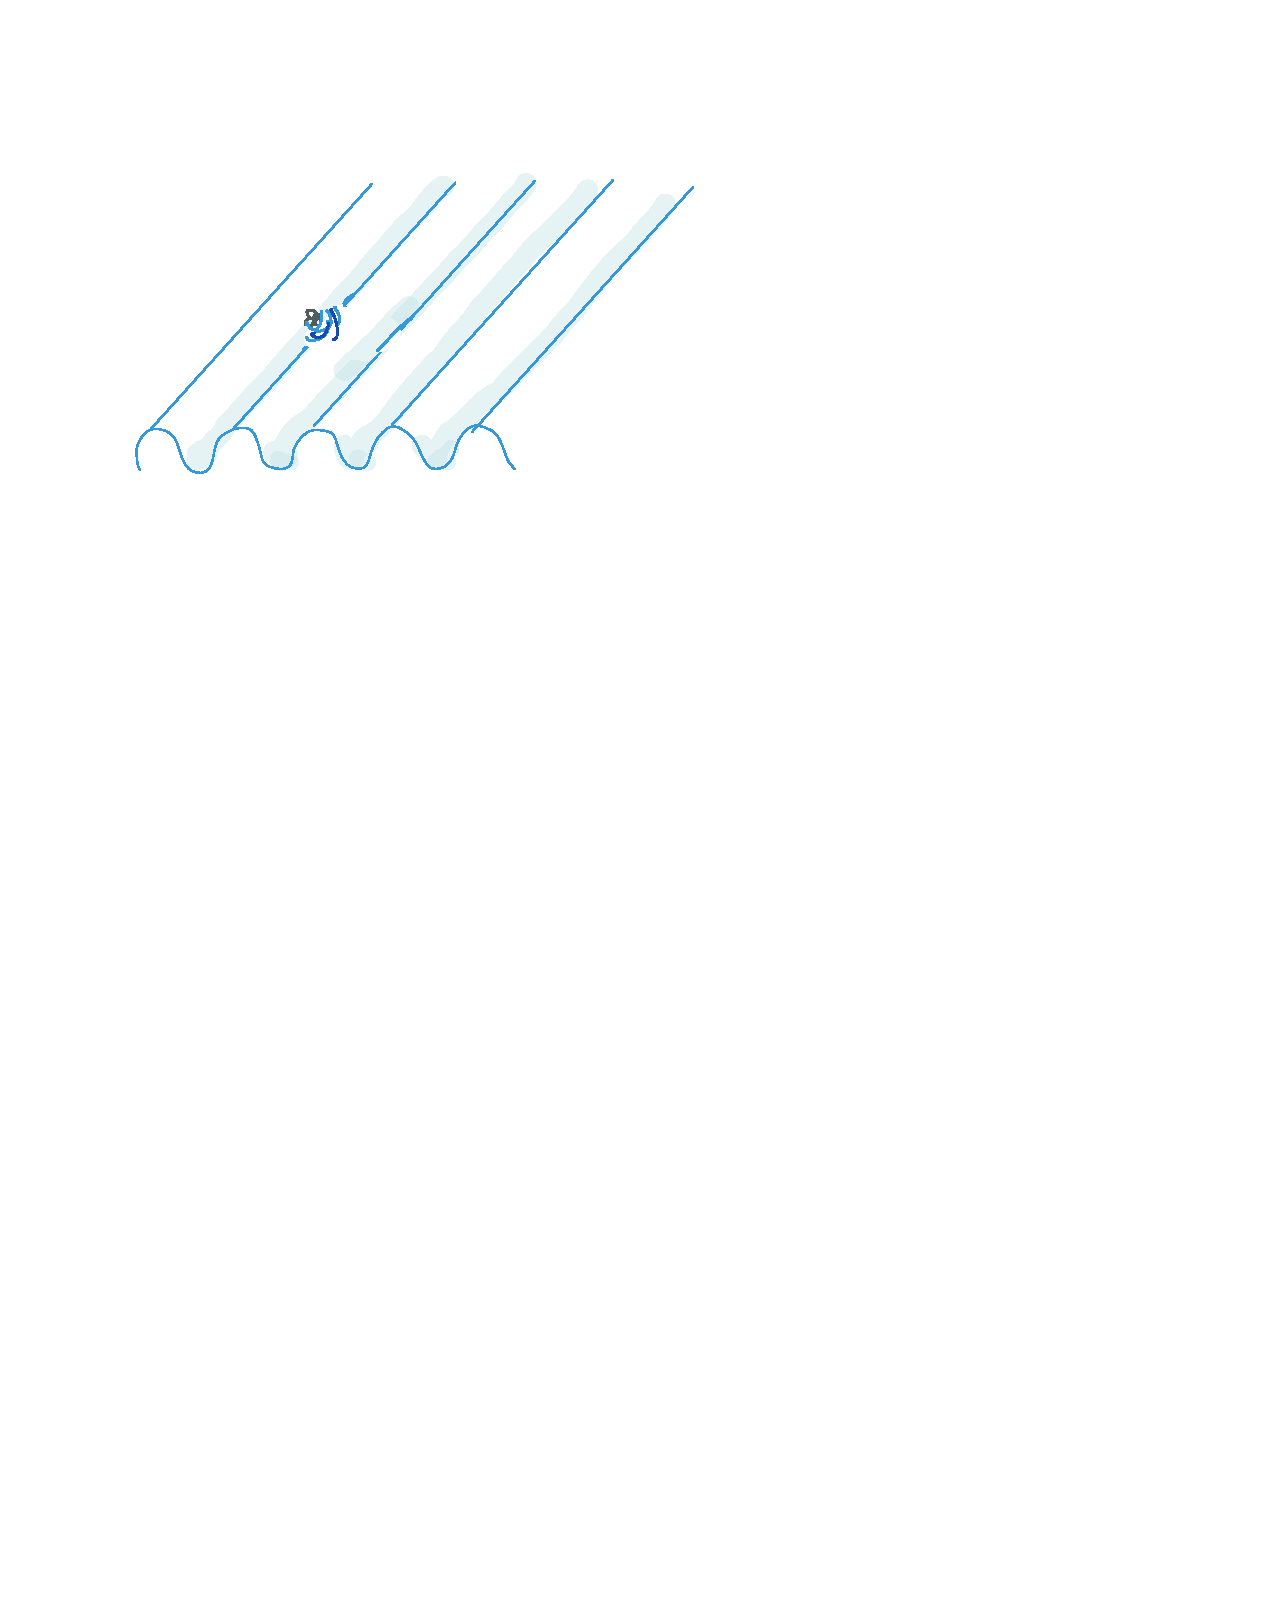
\includegraphics[width=\linewidth]{figures/waves_small.pdf}
        \caption{$\Delta x \ll \lambda$}
        \label{fig:subfig:waves:small}
    \end{subfigure}\;%
    \begin{subfigure}{0.3\textwidth}
    \centering
        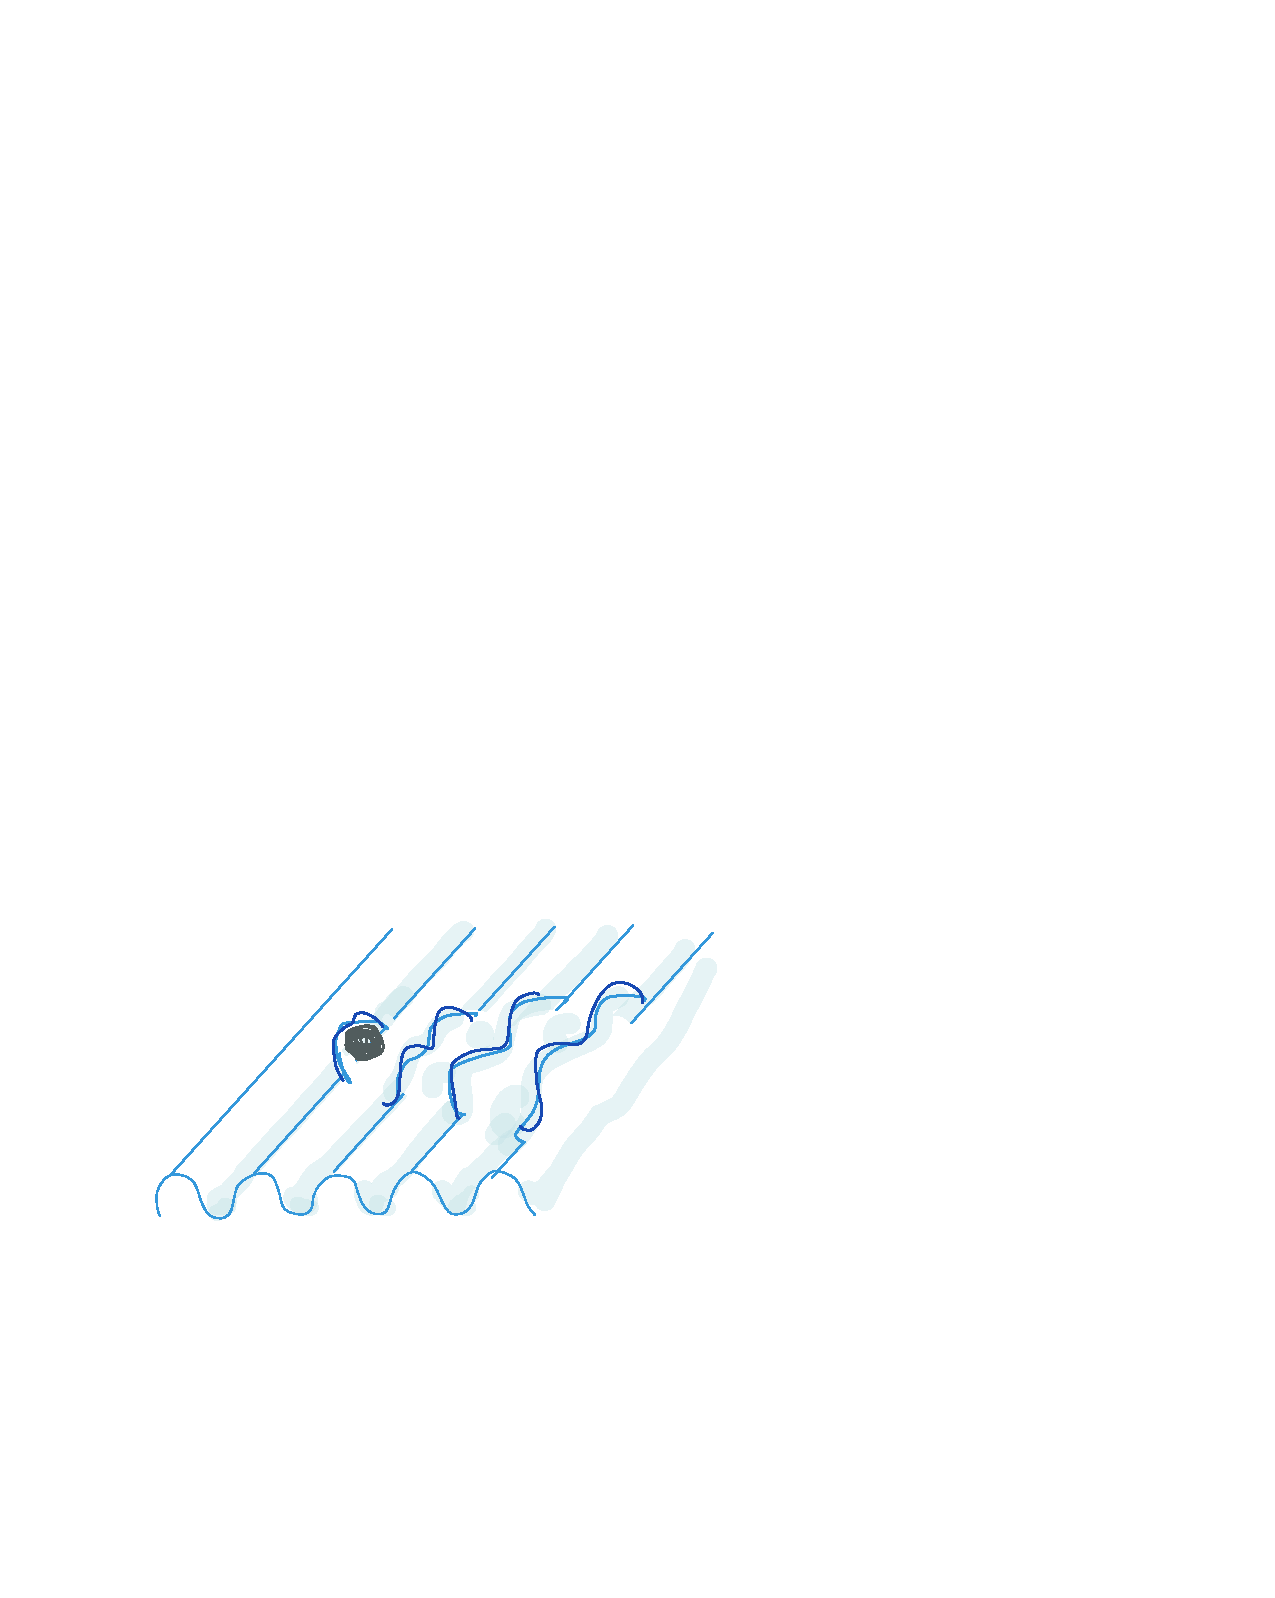
\includegraphics[width=\linewidth]{figures/waves_med.pdf}
        \caption{$\Delta x \sim \lambda$}
        \label{fig:subfig:waves:med}
    \end{subfigure}\;%
    \begin{subfigure}{0.3\textwidth}
    \centering
        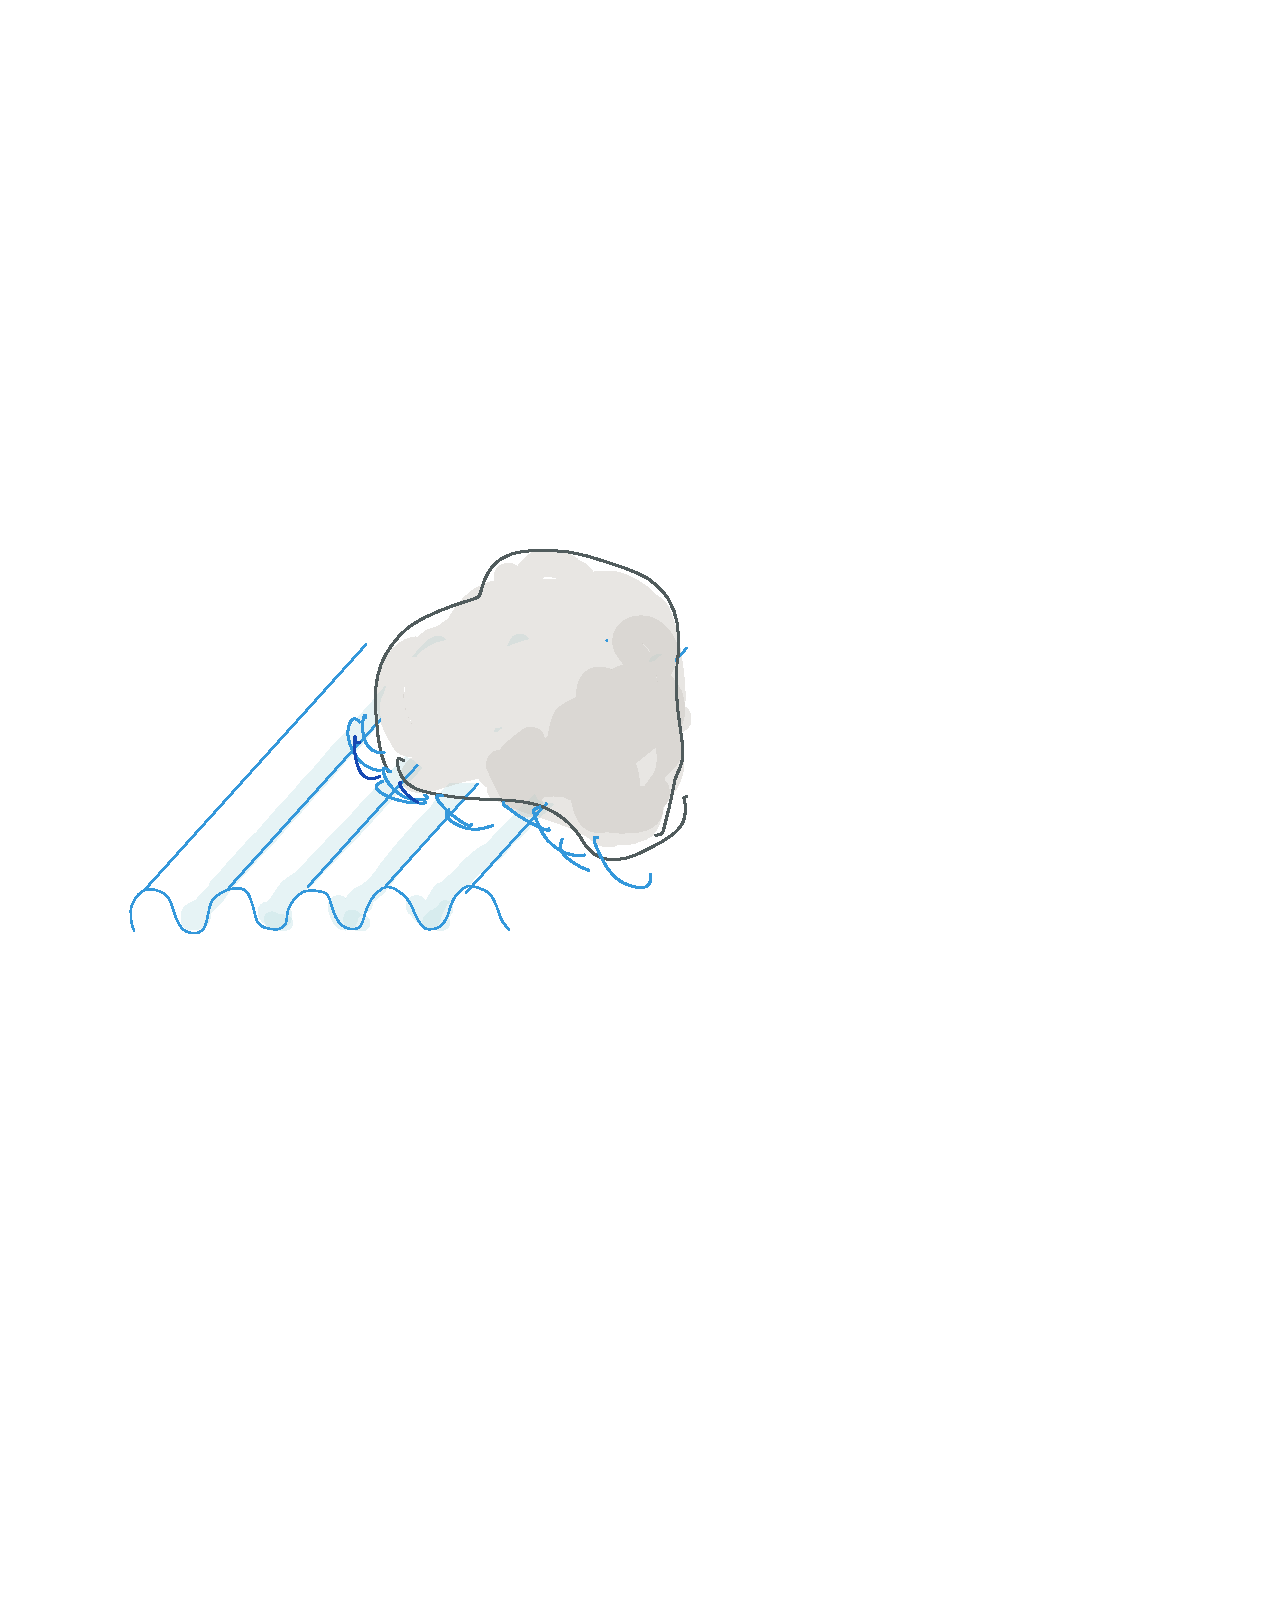
\includegraphics[width=\linewidth]{figures/waves_big.pdf}
        \caption{$\Delta x \gg \lambda$}
        \label{fig:subfig:waves:big}
    \end{subfigure}%
    \caption{The ability to probe features (like a rock) of typical scale $\Delta x$ depends on having a probe whose wavelength $\lambda$ is roughly on the order of $\Delta x$. If the scales are mismatched, then the waves are unable to resolve the $\mathcal O(\Delta x)$ features.}
    \label{fig:subfig:waves}
\end{figure}



\chapter{Rapid Review of Relativity}

We begin our study of particle physics with a lightning review of selected topics in special relativity and quantum mechanics.

\section{Kinematics}

The popular Einstein relation, $E = mc^2$, is actually the low [kinetic] energy limit of the `full' relation:
\begin{align}
    E^2 = m^2 c^4 + \vec{p}^2 c^2 \ .
    \label{eq:Einstein:relation:plus}
\end{align}
Equations that relate energy to momentum show up all over physics and have a special name: \textbf{dispersion relations}.\sidenote{As a student I always found this name intimidating because it would keep showing up in very different and increasingly advanced corners of physics. I felt like I must be missing something deep, especially since the word \emph{dispersion} did not seem to obviously fit. Historically, these relate wavelength to frequency. Recall that wave velocity is the product of wavelength and frequency---but wave velocity is purely a property in medium. Wavelength (or wave number) is directly related to momentum---think 
$\sin(kx)$---while frequency is directly related to energy---think $E=\hbar\omega$. These of these parameters are related to absorption (or decay) through complex analysis; these are the celebrated Kramers--Kr\"onig relations. We mention all of this to encourage you to look these ideas up and see how they connect; they are one of the deep threads in physics.} 
\begin{exercise}
It is obvious that \eqref{eq:Einstein:relation:plus} reproduces $E=mc^2$ when $\vec{p}=0$. Show that the leading order correction in the small-$\vec{p}$ limit is simply the non-relativistic kinetic energy of the particle. \textsc{Hint:} start by identifying the \emph{dimensionless} small parameter and Taylor expand.
\end{exercise}
In natural units we set $c=1$. In this relation, $m$ is the mass of a particle while $E$ and $\vec{p}$ are the energy and three-momentum respectively. Let us write this with the kinematic quantities on the same side of the equation:
\begin{align}
    m^2 = E^2 - \vec{p}^2 \ .
    \label{eq:on:shell}
\end{align}
A particle that satisfies this relation is said to be \textbf{on shell}\index{on shell} or \emph{physical}. Anticipating quantum mechanics, another way of saying this is that on shell particles are \emph{observable states}. Personally, I think of `on shell' states as being \emph{nice} states that are relatable to my ordinary human experiences. This is in contrast to \textbf{off shell} particles, which states that are \emph{not} on shell and are intrinsically quantum. Off shell states are not observable and do not make sense classically. 

A scattering process is one where some number of \emph{observed} initial state particles interact quantum mechanically and produce and \emph{observed} number of final state particles. These initial and final states must each be on shell and conserve energy and momentum. 
\begin{newrule}[Kinematics]
A \textbf{physical scattering process} is one with an on shell initial state and an on shell final state. This just means that each particle in the initial and final state are on shell. Furthermore, the total energy $E$ and total three-momentum $\vec{p}$ are conserved through the process. In equations:
\begin{align}
    E_\textnormal{in} &= E_\textnormal{out}
    &
    \vec{p}_\textnormal{in} &= \vec{p}_\textnormal{out}
    &
    m_i^2 = E_i^2 - \vec{p_i}^2 \ ,
\end{align}
where $i$ labels each of the external (initial or final) particles. Technically, we should also specify that $E_i>0$, but for us we can take this as an ``obvious'' fact.\sidenotemark Note that in this notation, $E_\textnormal{in}$ is the sum of the energies of all the initial state particles, and similarly for the other in/out quantities.
\end{newrule}\sidenotetext{From a group theory perspective, positive energy means that we are restricting to the \emph{orthochronus}\index{orthochronus} Lorentz group. This means that particles always move forward in time, no matter what reference frame we are in. The relation between energy positivity and direction in time should be clear from the time evolution operator, \eqref{eq:Ut:time:H} with $\hat H\to E$.}

Suppose you have a particle detector that measures the energy of a particle passing through it---this is called a \emph{calorimeter}. If you also know the mass of the particle, then you can also unambiguously determine the magnitude of the momentum, $|\vec{p}|$.  Alternatively, if you could separately measure the energy and the momentum of a particle, then you can unambiguously infer its mass. This is all obvious because you are using one Einstein relation to relate three variables---mass, energy, and momentum. 

\begin{exercise}
Suppose you have a process where one particle decays into two other particles; these particles do not necessarily have the same masses, but suppose you know all of the masses. You know the energy and momentum of the initial particle, $E_\textnormal{in}$ and $\vec{p}_\textnormal{in}$. You do not know, \emph{a priori}, the energies or momenta of the final state particles. How many unknown scalar quantities are there? How many constraint equations are there? \textsc{Hint}: recall that $\vec{p}$ is a vector with three separate quantities. Argue that there is generically \emph{no} solution to this system unless some parameters (e.g.\ the masses) are just right.
\end{exercise}

\begin{exercise}
Suppose you have a process where two particles come in, and two particles come out. The particles do not necessarily have the same mass, but you know all of the masses. If you know the energies of the initial particles, how many unknowns are there and how many constraint equations are there? Do you expect this system to have a solution? \textsc{Note}: for the purposes of this problem, assume that all energies are positive. This corresponds to satisfying the orthochronus constraint. If you are nervous about this, check that by increasing the energies of the initial particles you can make sure that the final state particles have positive energy. 
\end{exercise}


\section{Time Dilation and Length Contraction}

\begin{flipcomment}
This section is a very brief review of the main points. For a more systematic derivation, please see my Physics 17 lecture notes. 
\end{flipcomment}

My favorite refernece to appreciate the geometric structure of special relativity is the book \emph{Very Special Relativity}\autocite{bais2007very}.
\begin{marginfigure}%[th]
    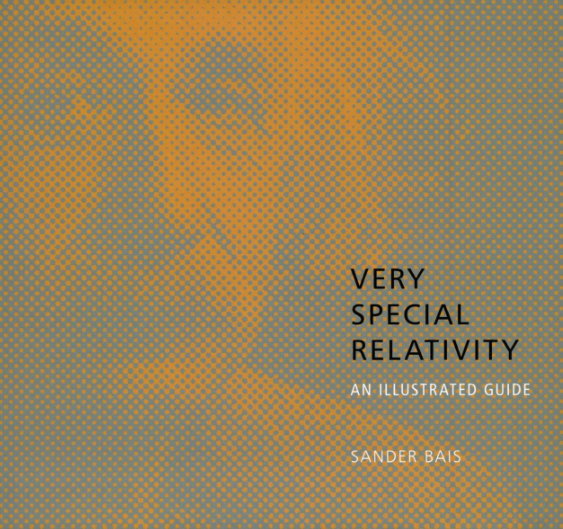
\includegraphics[width=.8\textwidth]{figures/vsr_cover.png}
    \captionsetup{font={scriptsize,sf}}
    \caption{How to learn special relativity.}
    \label{fig:VSR:cover}
\end{marginfigure}
It looks like a miniature coffee table book, but it is a perfect book for physics students who have completed their lower-level coursework.\sidenote{If you can derive every result in the book then you are ready to take general relativity. You should be able to do this over a winter break.}\sidenote{Do not confuse the title of this book with the Cohen--Glashow hypothesis, \arXiv{hep-ph/0601236}, which is a rather different thing.} Once you have mastered this, you can pick up your favorite general relativity textbook for a bit more of the mathematical formalism. Some suggestions: Hartle\autocite{Hartle:2003yu}, Schutz\autocite{schutz2009first}, and Carroll\autocite{Carroll:2004st}. I would be remiss not to also mention the beautiful and elegant tome known lovingly as \acro{MSW}\autocite{misner2017gravitation}; a book so beloved that it had its own 50$^\textnormal{th}$ anniversary celebration.\footnote{\url{https://www.youtube.com/watch?v=a-4-IPBNV60}}
\begin{marginfigure}%[th]
    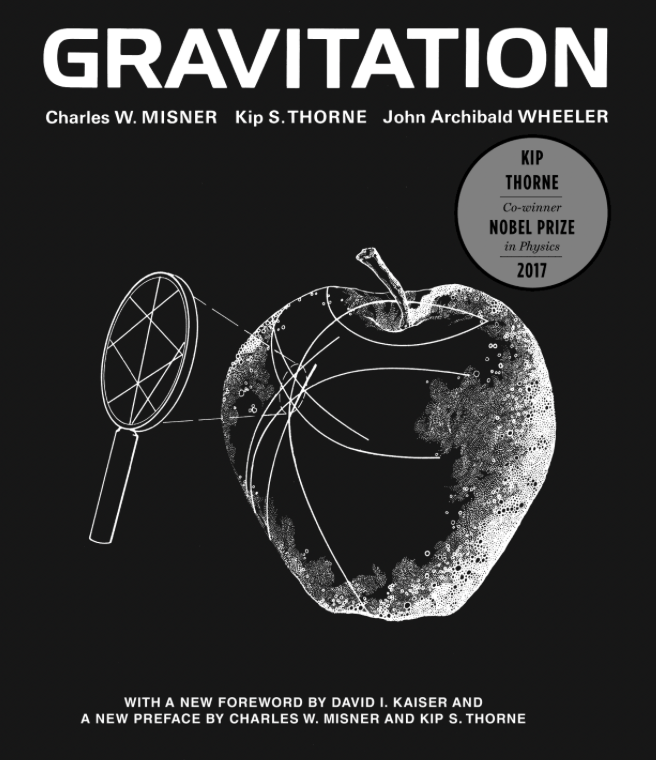
\includegraphics[width=.8\textwidth]{figures/MSW_cover.png}
    \captionsetup{font={scriptsize,sf}}
    \caption{Published 50 years ago---right around when the Standard Model was established---\tacro{MSW} is still one of the most insightful places to learn and re-learn relativity. }
    \label{fig:MTW:cover}
\end{marginfigure}

The key tenet of special relativity is that the speed of light is constant. You already know from \eqref{sec:units:dimensions} that this constant means that there is a natural conversion between space and time. Indeed, you should already be familiar with the two primary manifestations of this in mechanics:
\begin{itemize}
    \item Time dilation: We measure time to pass more slowly for objects moving relative to our reference frame.
    \item Length contraction: We measure the distance along the direction of motion to be shorter for objects moving relative to our reference frame. 
\end{itemize}
This is formalized with respect to the relative velocity\sidenote{In \tacro{SI} units we would say $\beta = v/c$.} $\beta = v$ and the factor
\begin{align}
    \gamma = \frac{1}{\sqrt{1-\beta^2}} \ .
\end{align}
\begin{exercise}
What is the range of allowed values of $\beta$? What is the range of allowed values for $\gamma$? What is the allowed range of the product $\gamma\beta$?
\end{exercise}
We, as observers, define a stationary reference frame with coordinates $t$ and $x$. For our purposes, let us assume a (1+1)-dimensional spacetime.\sidenote{This notation means one dimension of time and one dimension of space.} Suppose that there is another references frame that is moving at constant velocity relative to ours. Then an observer in that reference frame has a coordinate system $t'$ and $x'$. Fig.~\ref{fig:relativity:axes} plots the axes of this coordinate system on our coordinate system. 
\begin{marginfigure}%[th]
    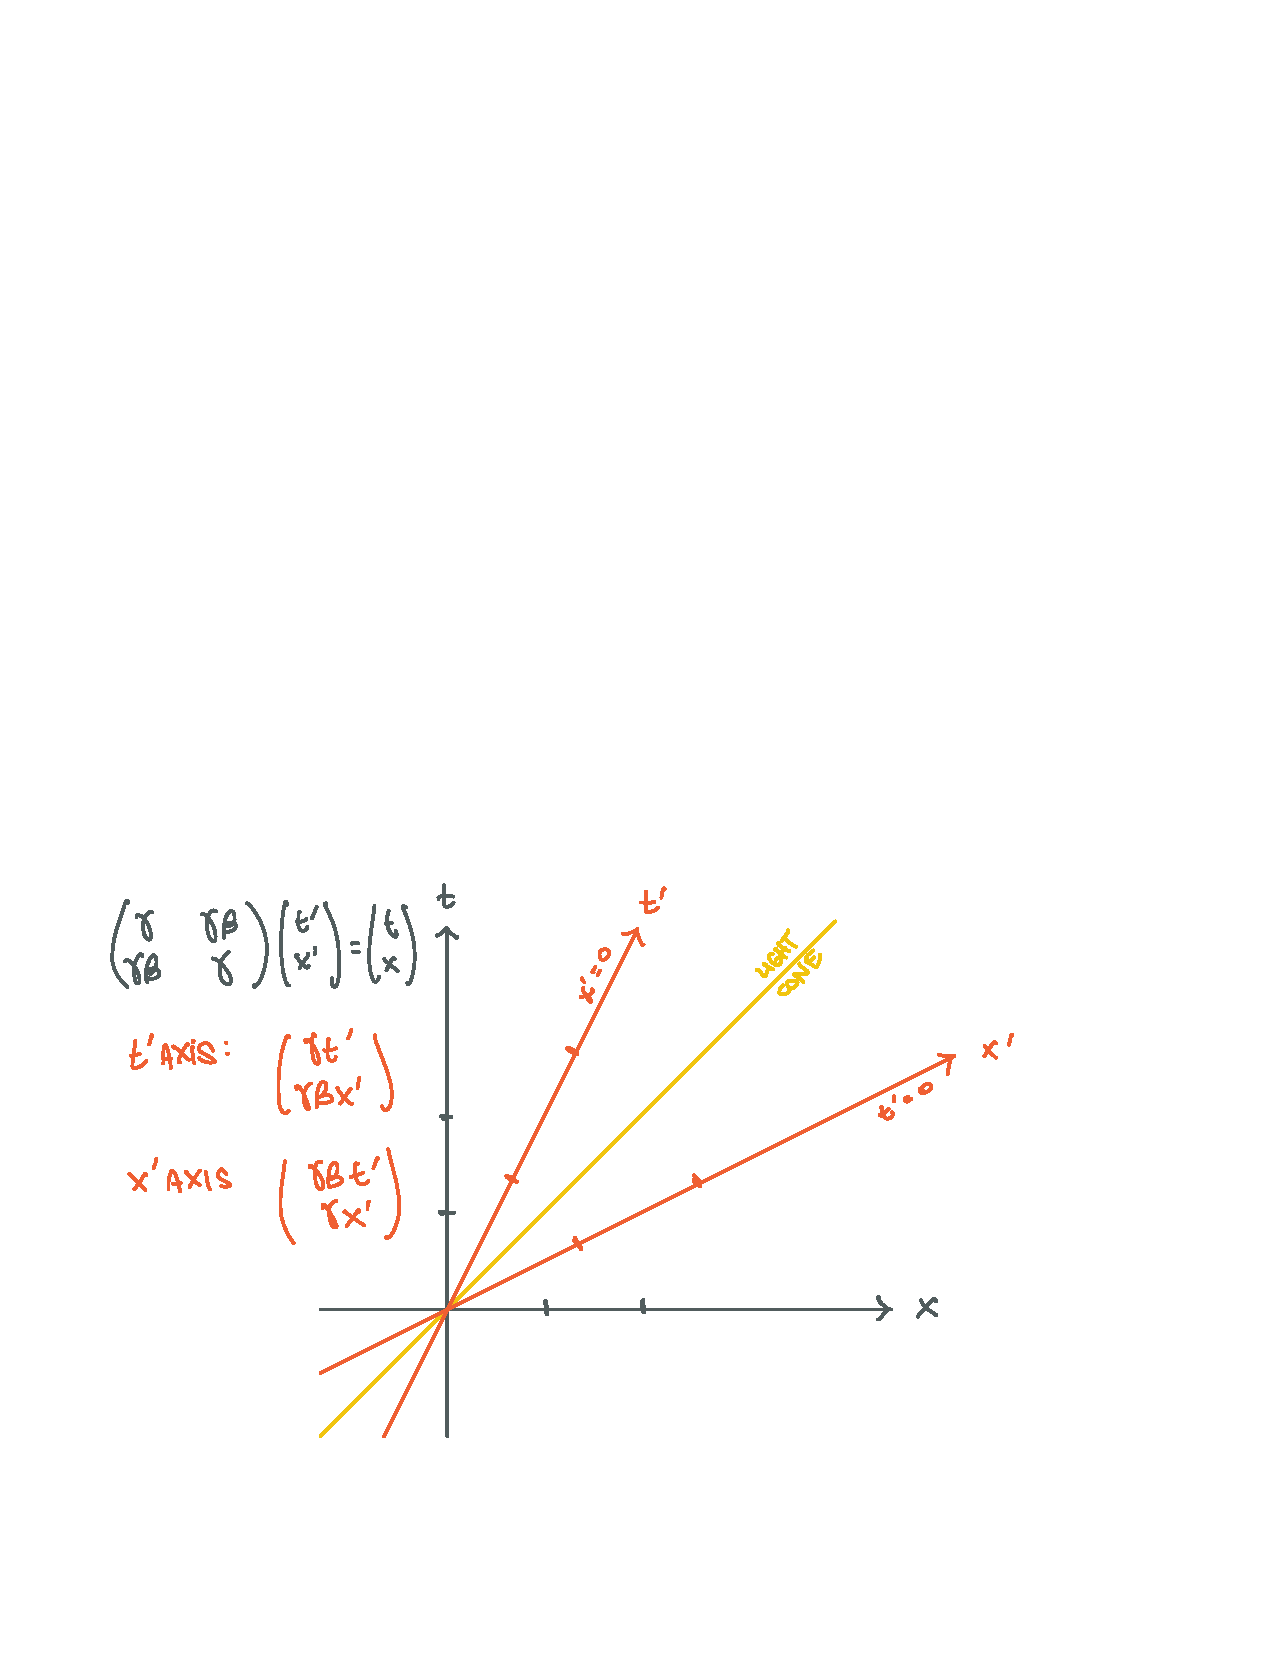
\includegraphics[width=\textwidth]{figures/rel_axes.pdf}
    \captionsetup{font={scriptsize,sf}}
    \caption{Coordinates of a boosted observer relative to our coordinates.}
    \label{fig:relativity:axes}
\end{marginfigure}
\begin{exercise}
Compare Fig.~\ref{fig:relativity:axes} to the spatial $x$--$y$ plane and the $x'$--$y'$ plane where the primed coordinates are those of an observer rotated by angle $\theta$ relative to the unprimed observer.
\end{exercise}
the coordinates are related by
\begin{align}
    t' &= \gamma t - \gamma\beta x &
    x' &= \gamma x - \gamma\beta t \\
    t &= \gamma t' + \gamma\beta x' &
    x &= \gamma x' + \gamma\beta t' 
    \ .
    \label{eq:Lorentz:2D:in:equations}
\end{align}
We realize that this is a linear system of equations,\sidenote{Recall that system of equations is linear if a \emph{linear combination} of solutions is also a solutions.} so we can write this as a matrix multiplication:
\begin{align}
    \begin{pmatrix}
        t\\
        x
    \end{pmatrix}
    =
    \begin{pmatrix}
        \gamma & \gamma \beta \\
        \gamma \beta & \gamma
    \end{pmatrix}
    \begin{pmatrix}
        t'\\
        x'
    \end{pmatrix} \ .
    \label{eq:Lorentz:2D:prime:to:unprimed}
\end{align}
\begin{exercise}
Show that 
\begin{align}
    \begin{pmatrix}
        t'\\
        x'
    \end{pmatrix}
    =
    \begin{pmatrix}
        \gamma & -\gamma \beta \\
        -\gamma \beta & \gamma
    \end{pmatrix}
    \begin{pmatrix}
        t\\
        x
    \end{pmatrix} \ .
\end{align}
You can do this either ``read it off' \eqref{eq:Lorentz:2D:in:equations} or apply the matrix inverse to both sides of \eqref{eq:Lorentz:2D:prime:to:unprimed}. Show that the two matrices are, indeed, inverses of each other.
\end{exercise}
\begin{exercise}
Confirm that \eqref{eq:Lorentz:2D:prime:to:unprimed} maps $x'$ and $t'$ axes to the $x$ and $t$ plane as shown in Fig.~\ref{fig:relativity:axes}.
\end{exercise}

% \begin{example}
% Suppose the boosted observer has a stick that they measure to be length $\ell'$. Because the observer and the stick are at rest relative to each other, we say that $\ell'$ is the \textbf{proper length} of the stick. That means in a time slice $\Delta t' = 0$ it observes a distance interval $\Delta x' = \ell'$. In our frame, we measure
% \begin{align}
%     \Delta t &= \gamma \beta \,\Delta \ell'
%     &
%     \Delta x &= \gamma \,\Delta\ell' \ .
% \end{align}
% It is helpful to define an origin where the origins of both reference frames coincide: $t_1 = t_1' = 0$ and $x_1 = x_1=0$
% \end{example}


\section{Indexology of Special Relativity}

\subsection{Upper Index}\label{sec:index:upper}

The unification of space and time is manifest in the formalism of \textbf{four vectors}\index{four vector}. At one level, this is a simple generalization of three-component vectors to four-component vectors. For example, an \emph{event} is a position $\vec{x}$ and a time $t$ and we can write it as a four-vector with an upper index:
\begin{align}
    x^\mu \equiv (x^0, x^1, x^2, x^3) = (t,x,y,z) \ .
\end{align}
There are several caveats that we should make at this point since they are not often stated out loud in textbooks:
\begin{itemize}
    \item We use the usual physicist's abuse of notation where we identify an object $x$ with a generic component, $x^\mu$. 
    \item It is conventional to index time with $\mu=0$. Some old texts use the antiquated notation $x^4$. For this reason in theories of extra dimensions it is conventional to label the extra dimension as $x^5$. 
    \item There is no such thing as a \emph{position vector}.\sidenote{I know a mathematician who was confused when the physics students in his calculus class kept talking about position vectors, as if the students were talking about unicorns. This may seem like nit picking, but it this insight is part of the underlying geometric picture built on fiber bundles. See \arXiv{hep-th/0611201} for a pedagogical introduction that should be accessible to students of this class with a bit of work.} This is because vector spaces have a special point, the origin $x^\mu = 0$. There is no such special point in spacetime. However, relative positions, $\Delta x^\mu = x_A^\mu - x_B^\mu$, are well defined vectors. 
\end{itemize}
In particle physics we do not often deal with (relative) position four vectors because our states are typically momentum eigenstates. Just as time and space are unified by $c=1$, so too are energy and momentum. These are combined into a four-momentum,
\begin{align}
    p^\mu \equiv (p^0, p^1, p^2, p^3) = (E, p^x, p^y, p^z) \ .
    \label{eq:fourmomentum:upper}
\end{align}
$p^\mu$ is the Fourier transform of $x^\mu$. It should not surprise you that we work with momentum eigenstates: these are the states that are eigenstates of the Hamiltonian by virtue of having a well defined energy. The on shell condition \eqref{eq:on:shell} then gives a well defined three-momentum magnitude.

Like any other vector space, linear combinations of vectors are also vectors. Recall that a linear combination of vectors is a sum of vectors that each may have some rescaling by a real number. For two vectors, this is:
\begin{align}
   (\alpha\vec{v}+\beta\vec{w})^i = \alpha v^i + \beta w^i \ .
\end{align}
We read this relation as: the $i^\textnormal{th}$ component of the vector $(\alpha\vec{v}+\beta\vec{w})$ is equivalent to the number given by the sum of two rescaled vector components: $\alpha$ times $v^i$ and $\beta$ times $w^i$. The coefficients $\alpha$ and $\beta$ are any real numbers. In this example we used the index $i$ to show that this is true for \emph{any} vector space, not just the space for four-vectors. We call the $\mu$ index\sidenote{In our convention, lowercase letters from the middle of the Greek alphabet are Lorentz indices.} a \textbf{Lorentz index} because it indexes the four directions of spacetime.

\begin{example}
For example, this means that conservation of energy and momentum in an interaction
\begin{align}
    \sum_{i = \textnormal{incoming}} p_{(i)}^\mu -
    \sum_{i = \textnormal{outgoing}} p_{(i)}^\mu = 0
    % \sum_{i = \textnormal{external}} p_{(i)}^\mu = 0
    \label{eq:conservation:four:momentum}
\end{align}
where $p_{(i)}^\mu$ is the $\mu$ component of the four-momentum of the $i^\textnormal{th}$ particle in an interaction. By convention, incoming particles have positive signs and outgoing particles have negative signs.  Setting $\mu=0$ in \eqref{eq:conservation:four:momentum} tells us that the sum of all energies going into an interaction must match the sum of all energies coming out of the interaction. Similarly, setting $\mu=1$ tells us that momentum in the $x$-direction is conserved. 
\end{example}


Vectors with upper indices have equivalent names: column vectors, contravariant vectors, kets. To be very precise mathematically: the vector is the object $\vec{v}$, while $v^\mu$ is the $\mu^\textnormal{th}$ component of the vector. Physicists like to blur the line here and will write a \emph{generic component} of a vector $v^\mu$ to interchangeably mean the vector as a whole or the specific component.\footnote{Roger Penrose proposes formalizing this shorthand in what is called \emph{abstract index notation}. A good online discussion is this one: \url{https://math.stackexchange.com/questions/455478/}}\sidenote{What is implicit here is an understood set of basis vectors $\vec{e}_\mu$ such that $\vec{v} = v^\mu \vec{e}_{\mu}$. These basis vectors carry the abstract vector-ness of $\vec{v}$ while $v^\mu$ can be thought of as a set of numbers. Refer to my Physics 17 notes to see this exhaustively.}

\subsection{Lower Index}\label{sec:index:lower}

Upper index vectors also have lower-index counterparts. These also have many equivalent names: row vectors, covariant vectors, bras, one-forms. There is a mathematical machine called a \textbf{metric}\index{metric} that can raise or lower indices. For now let us assume that lower indexed objects exist. In fact, often momentum is written with a lower index:
\begin{align}
    p_\mu = (E, p_x, p_y, p_z) \ . 
    \label{eq:fourmomentum:lower}
\end{align}
As introduced, this as a separate object than the upper index four-momentum \eqref{eq:fourmomentum:upper}. However, the metric gives a concrete relation between the two:
\begin{align}
    p_\mu &\equiv (E, -p^x, -p^y, -p^z)
    &
    p^\mu &\equiv (E, -p_x, -p_y, -p_z) \ .
\end{align}
To go from upper to lower Lorentz index, evidently there is simply a minus sign on the spatial ($\mu=1,2,3$) components. 






\subsection{Summation Convention}

We adopt \textbf{summation convention}\index{summation convention} where:
\begin{newrule}[Summation convention]
In an expression where an upper and a lower index are written with the same character, it is \emph{understood} (left unwritten) that one should sum over these indices. We say that these indices are \textbf{contracted}\index{contract}.
\end{newrule}
The key example for us is the contraction of an upper-index four momentum and its lower-index counterpart:
\begin{align}
    p^\mu p_\mu = p_\mu p^\mu = E^2 - p_x^2 - p_y^2 - p_z^2 = E^2 - \vec{p}^2 \ .
\end{align}
Using this convention, the on shell condition \eqref{eq:on:shell} is\sidenote{Note that $p^2 = p_\mu p^\mu$ while $\vec{p}^2 = p_x^2 + p_y^2 + p_z^2$. }
\begin{align}
    p^2 \equiv p^\mu p_\mu = m^2 \ .
\end{align}
Contracted indices are effectively not indices: $p^2 = p^\mu p_\mu$ is a \emph{number} and not a four-vector or other type of tensorial object. 

Evidently the way we are writing our theory tells us that the unification of space and time (energy and momentum) is also a statement about the on shell condition for particles. 


The following examples are completely general for any type of linear transformation from a vector space to itself. 
\begin{example}
A linear transformation (``matrix'') $M\aij{i}{j}$ is a \emph{linear map} that takes vectors into vectors. For example, the transformation $M=M\aij{i}{j}$ acts on a vector $\vec{v} = v^i$ as $M\vec{v}$ with components given by
\begin{align}
    (M\vec{v})^i = \sum_k M\aij{i}{k}v^k = M\aij{i}{1}v^1 + M\aij{i}{2}v^2 + \cdots \ .
    \label{eq:matrix:on:vector:eg}
\end{align}
Observe that the matrix must have an upper index and a lower index. Summation convention tells us that the lower index allows the matrix to contract with the  index of the vector it acts on. The upper index of the matrix corresponds is `leftover' and is the free index of the resulting vector, $M\vec{v}$.
\end{example}


\begin{example}
In \eqref{eq:matrix:on:vector:eg} the index $k$ is contracted. We may rewrite this equation using summation convention as
\begin{align}
    (M\vec{v})^i = M\aij{i}{k}v^k \ .
\end{align}
\end{example}




\section{Lorentz Transformations}\label{sec:Lorentz:transformations}

How do you relate vector quantities between different reference frames? A particle may have some four momentum\sidenote{We write $p$ to mean the abstract four-vector without specifying its components. We skip the `physics notation' of writing $p^\mu$ for clarity.} $p$. The \emph{components} of $p$ depend on the reference frame of the observer. We measure the components to be $p^\mu = (p^0, p^1, p^2, p^3)$. Another observer in another reference frame measures components $p'^\mu=(p'^0, p'^1, p'^2, p'^3)$. These components are related by a \textbf{Lorentz transformation}\index{Lorentz transformation} \eqref{eq:Lorentz:2D:prime:to:unprimed}:
\begin{align}
    p^\mu = \Lambda\aij{\mu}{\nu}p'^\nu \ .
\end{align}
If we align the spatial parts of each observer's coordinate system so that their relative motion is in the $z$ direction, then the components of the Lorentz transformation are
\begin{align}
    \Lambda\aij{\mu}{\nu} =
    \begin{pmatrix}
        \gamma & & & \beta\gamma\\
        & 1 & &  \\
        & & 1 &  \\
        \beta\gamma &  &  & \gamma
    \end{pmatrix}
    \ . 
    \label{eq:Lorentz:in:z}
\end{align}
This is simply what we showed in \eqref{eq:Lorentz:2D:in:equations}, extended to the $4\times 4$ case. You should think about this as an analog of the rotation matrix in Euclidean space.\sidenote{The relation is as follows. Rotations are the isometries of Euclidean space: they are the transformations that preserve the dot product. Lorentz transformations are the isometries of Minkowski space: they are the transformations that preserve the metric. In both cases, the isometries are the allowed transformations that preserve the spacetime structure as encoded by the metric.} Here $\beta$ is the relative velocity between the two frames. 
\begin{exercise}
Check that \eqref{eq:Lorentz:in:z} is a transformation from frame $\mathcal O'$
 to frame $\mathcal O$, where $\mathcal O'$ is moving in the $+\hat{z}$ direction relative to the $\mathcal O$. Show that the inverse of $\Lambda$ simply swaps the sign of $\beta$. 
\end{exercise}
\begin{example}
A nice way to see the relation between Lorentz transformations and boosts is to note that we may write the boost parameter as \textbf{rapidity}\index{rapidity} $\eta$ defined through the identification:
\begin{align}
    \Lambda[\eta] = 
    \begin{pmatrix}
        \cosh \eta & \sinh \eta \\
        \sinh \eta & \cosh \eta
    \end{pmatrix}
    =
    \begin{pmatrix}
        \gamma & \beta\gamma \\
        \beta \gamma & \gamma
    \end{pmatrix} \ .
\end{align}
Compare this to a rotation matrix,
\begin{align}
    R(\theta) &=
    \begin{pmatrix}
        \phantom{+}\cos \theta & -\sin\theta \\
        \phantom{+}\sin \theta & \phantom{+}\cos\theta
    \end{pmatrix} \ .
    \label{eq:eg:rotations}
\end{align}
Observe the key relations:
\begin{align}
    \cosh^2 \eta - \sinh^2 \eta &= 1\\
    \cos^2 \theta + \sin^2 \theta &=1 \ .
\end{align}
Here we appreciate the critical minus sign that is the difference between space and time.\sidenotemark
\end{example}
\sidenotetext{The connection between Lorentz transformations and rotations is further explicit in the so called Pauli-metric formalism where the time-component of a four-vector is \emph{imaginary}. In that formalism the metric is proportional to the identity and both Lorentz transformations and rotations take the form \eqref{eq:eg:rotations}.}

What about the transformation of lower index objects, like $p_\mu$? We can motivate based on what we know physically. But first, it is useful to review the case of simple rotations:
% 
\begin{example}[Transformation of row vectors]\label{eg:row:vector:transform}
Consider a Euclidean three-vector $\vec{v} = (v^x, v^y, v^z)^\trans$ and a Euclidean row vector, $\row{w} = (w_x, w_y, w_z)$. You know that the contraction these two objects is a number that is \emph{invariant}.
\begin{align}
    \row{w}\vec{v} = w_xv^x + w_y v^y + w_z v^z .
\end{align}
In fact, if $\row{w} = \vec{w}^\trans$, then $\row{w}\vec{v}$ is simply the inner product $|\vec{w}||\vec{v}|\cos\theta$. At any rate, the contraction $w_i v^i$ carries no indices and is a pure scalar quantity. That means it does not transform under rotations. However, we know that $\vec{v}$ \emph{does transform under rotations},
\begin{align}
    \vec{v}&\to R(\theta)\vec{v} 
    \ ,
\end{align}
with $R(\theta)$ given in \eqref{eq:eg:rotations}.
That means $\row{w}$ should also transform in a way to compensate the $\vec{v}$ transformation and keep $\row{w}\vec{v}=w_iv^i$ constant. Call this transformation $S(\theta)$. By the rules of matrix multiplication, $S(\theta)$ must act from the right:
\begin{align}
    \row{w} \to \row{w}S(\theta) \ \,
\end{align}
but from the index perspective the order does not matter:
\begin{align}
    w_i \to w_i S(\theta)\aij{i}{j} =  S(\theta)\aij{i}{j} w_i \ .
    \label{eq:order:of:terms:in:summation}
\end{align}
This is because each term in the sums on the right-hand sides of \eqref{eq:order:of:terms:in:summation} are just multiplication of two numbers. \emph{Make sure you understand this.}

The statement that $\row{w}\vec{v}$ is constant under rotations is
\begin{align}
    \row{w}\vec{v} \to \row{w}S(\theta)R(\theta)\vec{v}
    = 
    R(\theta)\aij{i}{\ell} S(\theta)\aij{k}{i} w_k v^\ell
\end{align}
so that we requre:
\begin{align}
      R(\theta)\aij{i}{\ell} S(\theta)\aij{k}{i}
      =
      S(\theta)\aij{k}{i}R(\theta)\aij{i}{\ell}
      =
      \delta\aij{k}{l} \ ,
      \label{eq:SR:RS:inverses}
\end{align}
or in other words, as matrices, $S(\theta)R(\theta) = 1$. Note that while it turns out to also true that $R(\theta)S(\theta) = 1$, \eqref{eq:SR:RS:inverses} is \emph{only} telling us that $S(\theta)R(\theta) = 1$ because when we write this index contraction was a matrix multiplication, the order matters: we have to make sure contracted indices are consecutive.

We thus conclude that
\begin{align}
    S(\theta) = R(\theta)^{-1} = R(-\theta) = R(\theta)^\trans \ .
\end{align}
So we demonstrate something very important: row vectors like $\row{w}$ `rotate oppositely' from column vectors like $\vec{v}$.
\end{example}

The lesson from the above example is that lower indexed objects transform with the \emph{inverse transformation} as upper indexed objects. Thus if $p^\mu \to \Lambda\aij{\mu}{\nu}p^\nu$, we must have
\begin{align}
    p_\mu \to (\Lambda^{-1})\aij{\nu}{\mu} p^\nu\ .
\end{align}
Check to make sure that you agree with the position of the indices. It is $(\Lambda^{-1})\aij{\nu}{\mu}$, not $(\Lambda^{-1})_{\mu}^{\phantom{\mu}\nu}$. Refer back to Example~\ref{eg:row:vector:transform} if that is not clear.



\section{Example: Muon Decay}

Cosmic rays can produce muons when they hit the upper atmosphere about 10 kilometers above the surface of the Earth.\sidenote{This sub-section is copied from my Physics 17 (2023) notes and is adapted from an example in Griffiths.} These muons are highly relativistic, with a velocity of $\beta = 0.9999$. See Fig.~\ref{fig:muons}. We know from laboratory experiments that the lifetime of a muon \emph{at rest} is 2 microseconds. Based on the simple estimate $d=c\tau \approx 600$~meters, we would not expect any muons to reach the surface of the Earth. However, not only do large cosmic ray telescopes have dedicated muon detectors, but you can make your own citizen science muon detector\sidenote{\url{https://muonpi.org}}. What gives?
\begin{marginfigure}%[tb]
    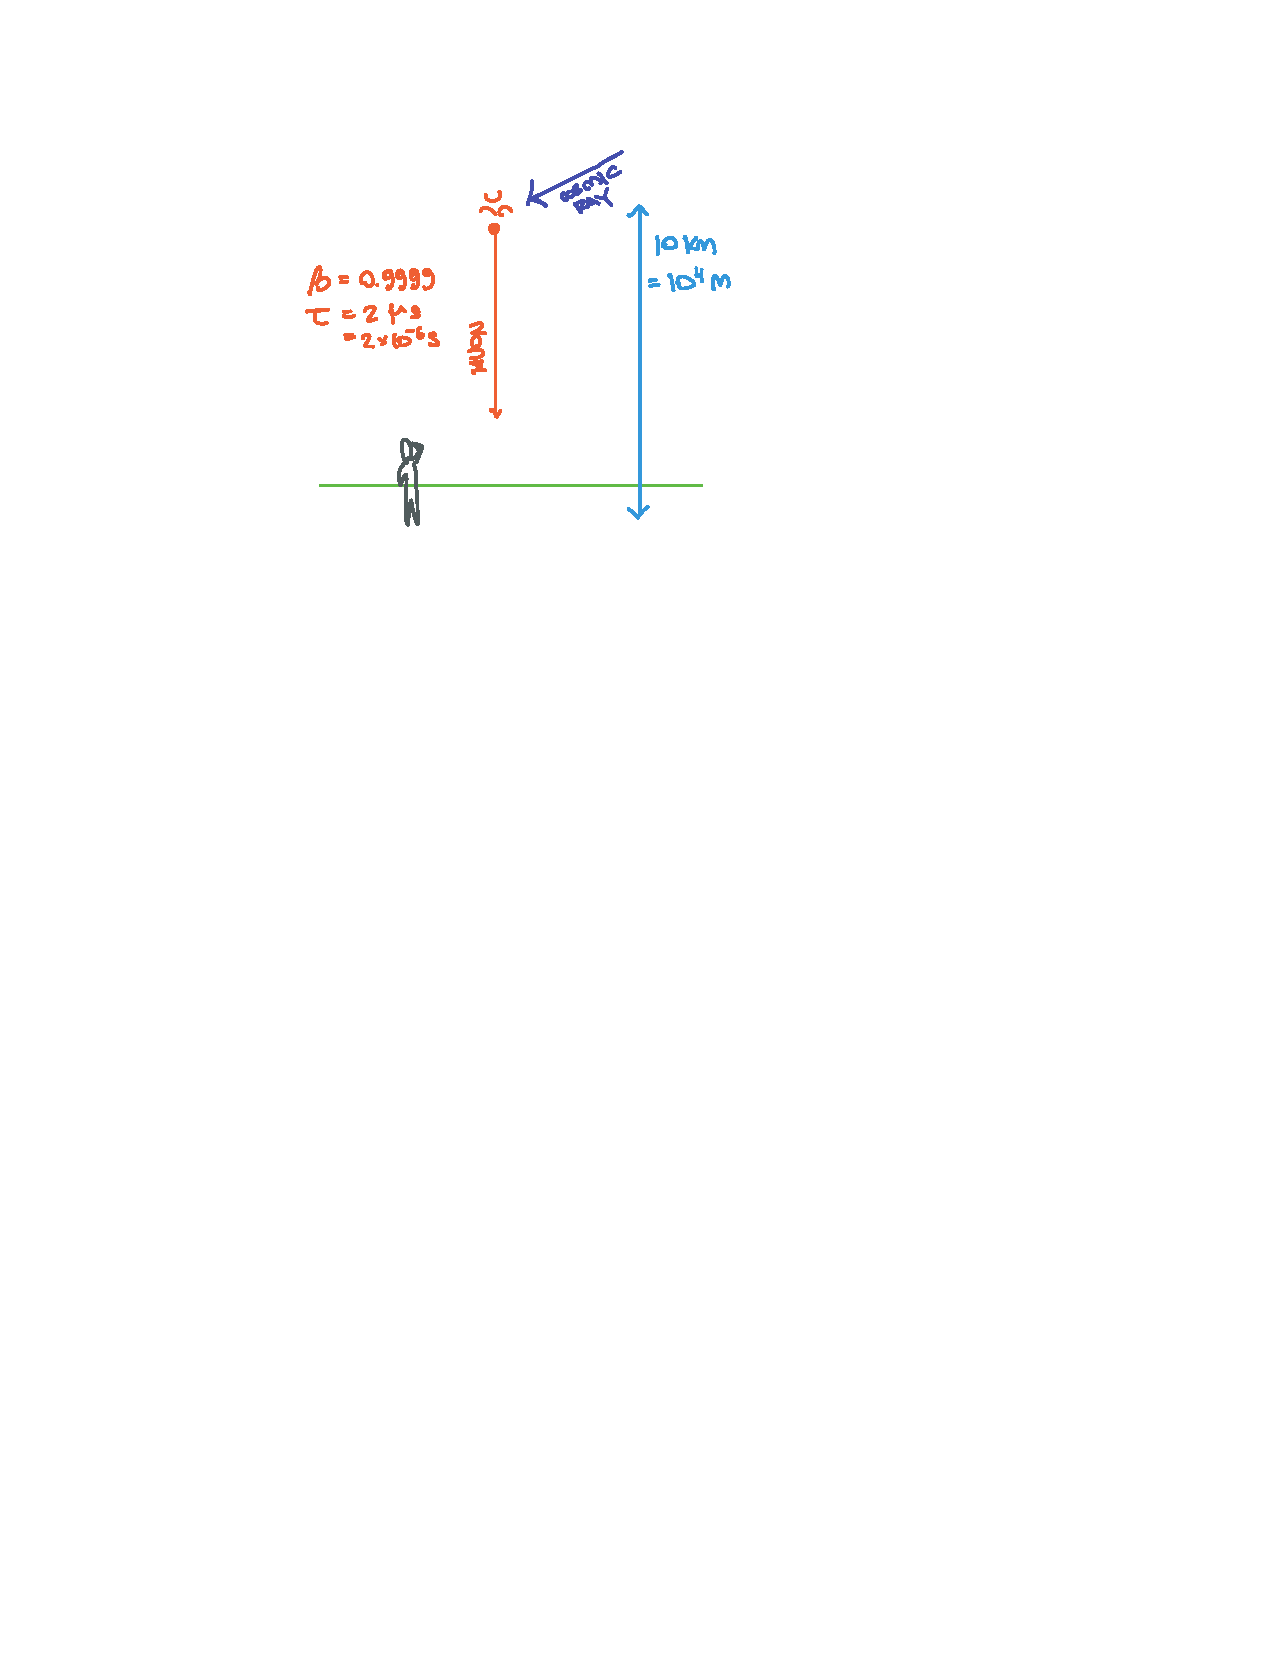
\includegraphics[width=\textwidth]{figures/muon.pdf}
    \captionsetup{font={scriptsize,sf}}
    \caption{Very technical sketch of a muon produced in the upper atmosphere heading towards earth. \label{fig:muons}} 
\end{marginfigure}
Here are the facts:
\begin{itemize}
    \item Both the observer on Earth and the muon agree that their relative velocity is $|\beta| = 0.9999$. 
    \item The muon's lifetime is known in the muon's rest frame. 
    \item The distance from the surface of the Earth to the upper atmosphere is known in the Earth's rest frame. 
\end{itemize}
The Lorentz transformation between the muon frame and the observe frame mix up space and time separations. We can only express the distance or time that the muon travels by calculating in the same reference frame. 

% \begin{figure}[tb]
%     \centering
%     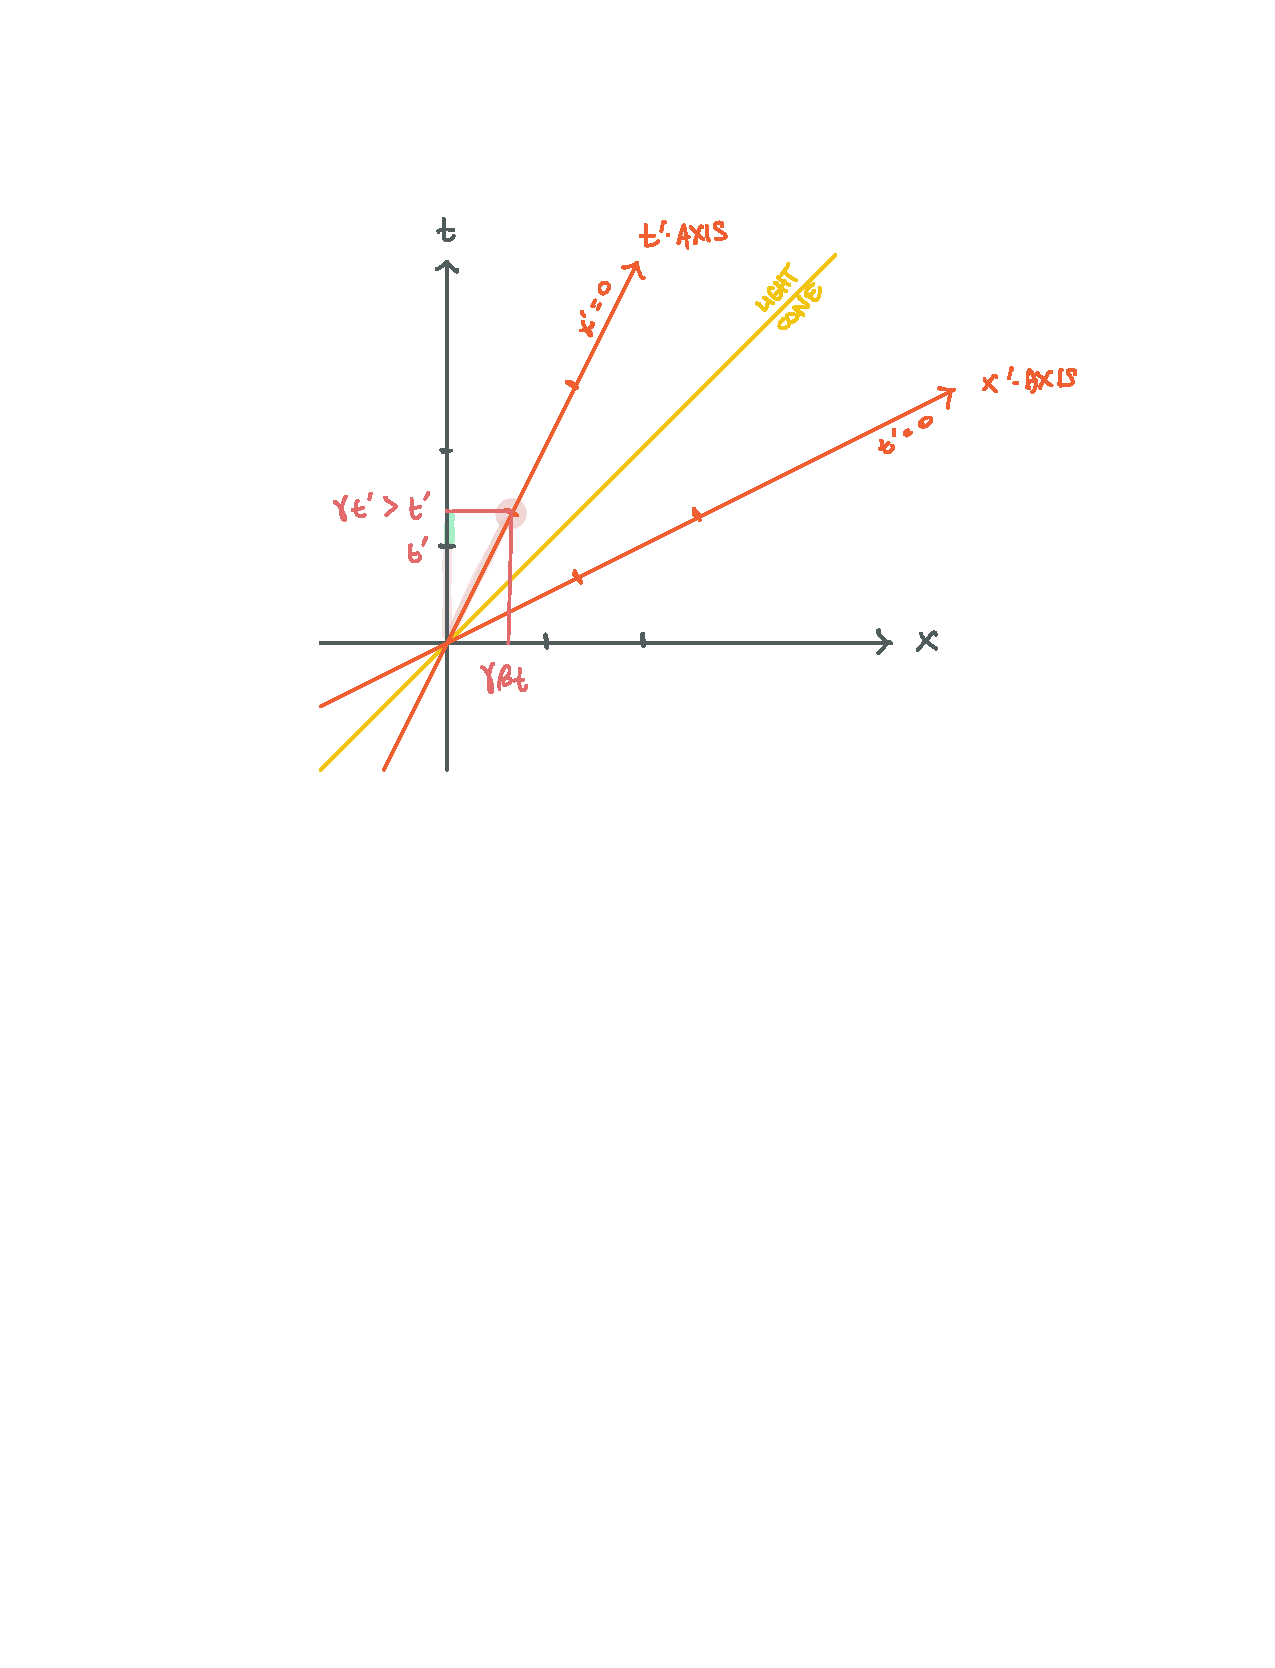
\includegraphics[width=.48\textwidth]{figures/rel_time_dil.pdf}
%     \quad
%     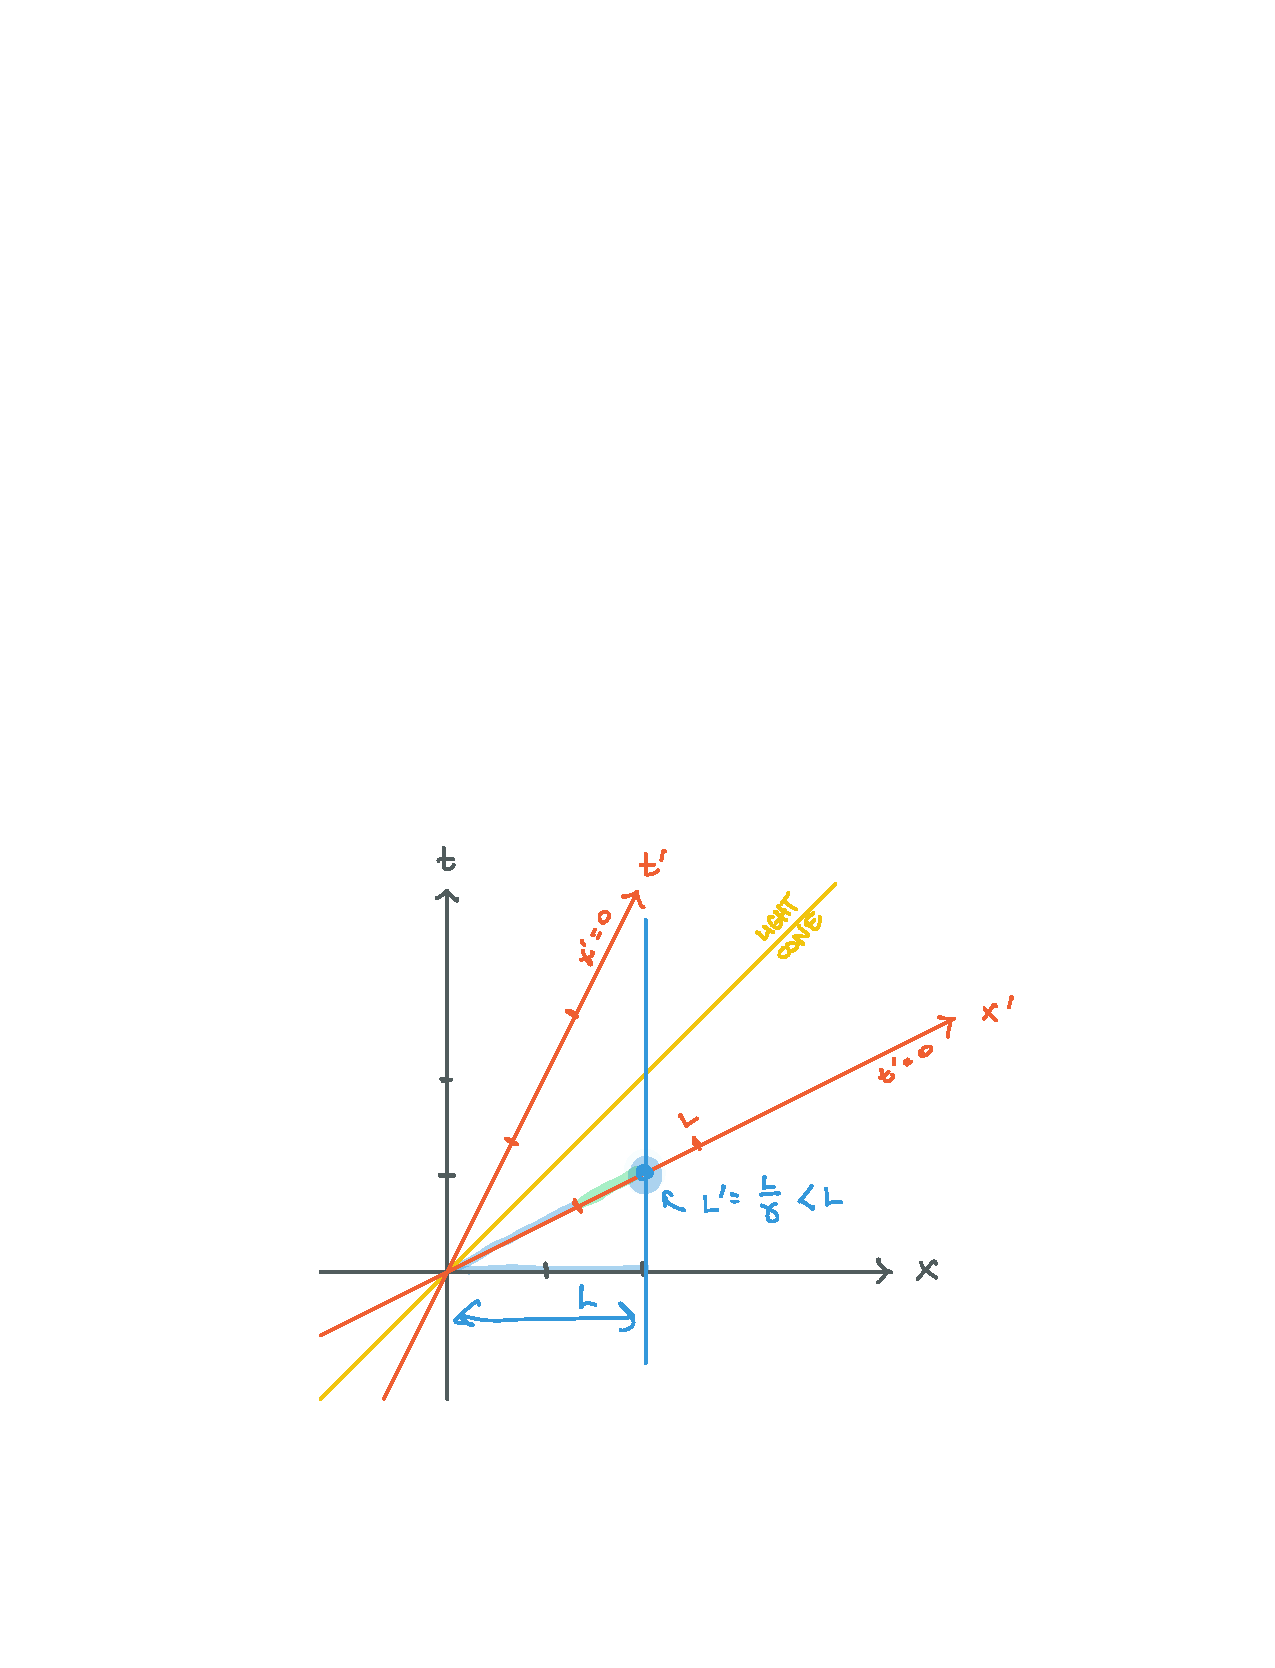
\includegraphics[width=.48\textwidth]{figures/rel_len_contractino.pdf}
%     \caption{Left: the muon's lifetime is time-dilated in the Earth's frame. Right: the distance from the surface of the Earth to the upper atmosphere is length contracted in the muon's frame. }
%     \label{fig:re:dilation}
% \end{figure}

First let us consider calculating everything in the Earth's reference frame. This is shown on the left of Fig.~\ref{fig:re:dilation}. This means we have to take the muon's lifetime in the muon's rest frame and convert it into a lifetime in the Earth's frame. In the muon's frame the lifetime is simply 
\begin{align}
    \Delta x'^\mu &= 
    \begin{pmatrix}
    \tau \\ 0     
    \end{pmatrix} \ 
    &
    \Delta x^\mu &=
    \begin{pmatrix}
    \gamma \tau \\ \gamma\beta \tau    
    \end{pmatrix} \ ,
\end{align}
where we have noticed that the muon lifetime is a displacement along the $t'$ axis used our results in \eqref{eq:Lorentz:2D:prime:to:unprimed}. We find that the lifetime in the Earth's frame is actually larger than the lifetime in the muon rest frame: $t = \gamma \tau$. There is also a spatial component, but this is no surprise: in the Earth frame the muon is moving, so when the muon decays it is in a different position. 

How much is the muon's lifetime \emph{time dilated}? We plug $\beta$ into the expression for $\gamma = (1-\beta^2)^{-1/2}$. We find\footnote{There's a cute trick here: $\beta^2 = (1-\epsilon)^2 \approx 1- 2\epsilon$ by Taylor expanding in the small number $\epsilon = 10^{-4}$.} that to one significant figure, $\gamma = 100$. This means that the time for the muon decay in the Earth's frame is $2\times 10^-4$~seconds, which means that it travels approximately $d=60~$km, which is larger than the distance from the upper atmosphere to the surface. As a sanity check: this is exactly the value in the spatial component of $\Delta x^\mu$.

Great: so one story is that relativistic muons have lifetimes that are much larger than their at-rest lifetime. This means that to the observer on earth, the muon simply lives longer than we would expect from measurements of muons at rest. There are, however, (at least) two sides to every good story. What does the muon see?

In the muon's rest frame, the muon \emph{knows} that it goes \emph{kaput} in 2~microseconds. It sees the surface of the Earth approaching it with velocity $\beta = 0.9999$. By now you can guess that must change: the measurement in the Earth's frame---that the height of the upper atmosphere is 10~km---must be different in the muon's frame. And in fact, the muon must measure the distance of the rapidly approaching Earth to be much smaller than 10~km. How does this \emph{length contraction} work? 

We show this on the right side of Fig.~\ref{fig:re:dilation}.
\begin{marginfigure}
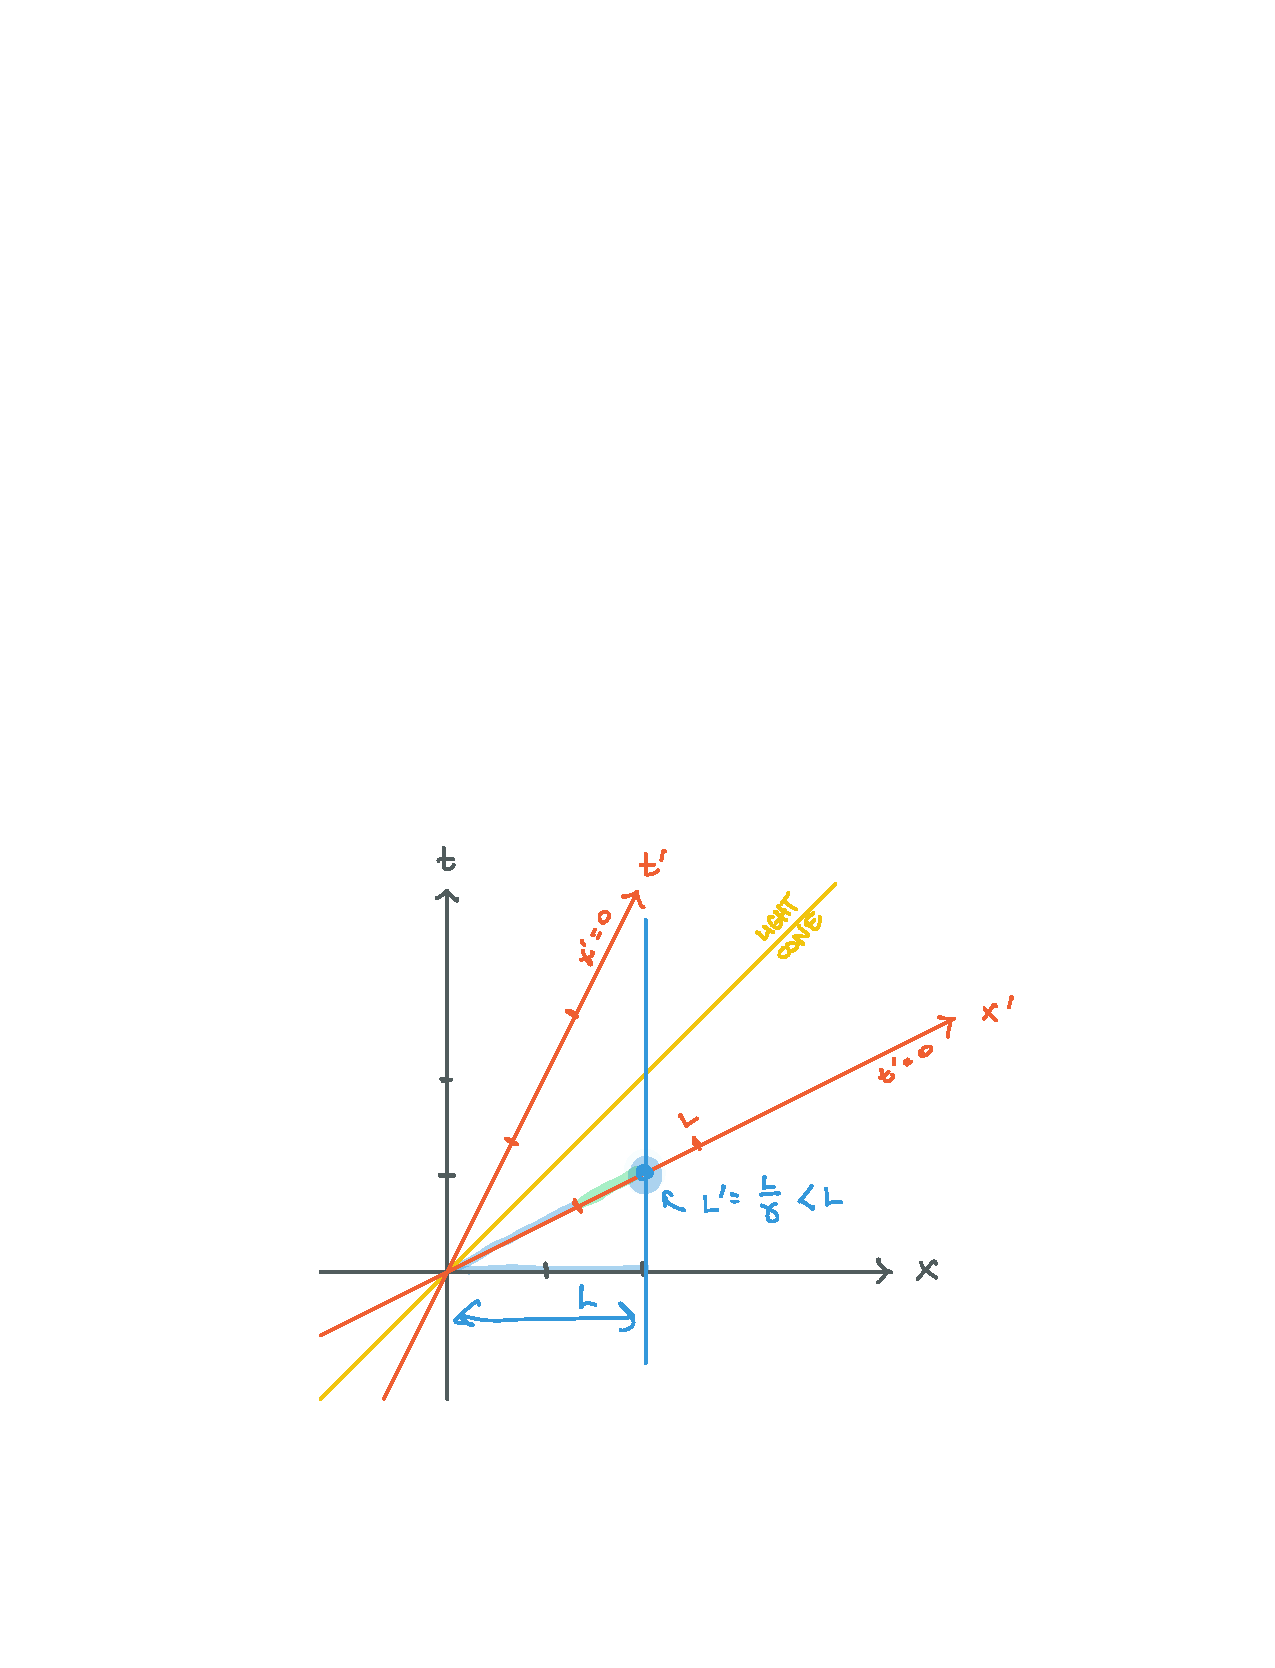
\includegraphics[width=\textwidth]{figures/rel_len_contractino.pdf}
\captionsetup{font={scriptsize,sf}}
\caption{The distance from the surface of the Earth to the upper atmosphere is length contracted in the muon's frame.
    \label{fig:re:dilation}
}
\end{marginfigure}
Note that now we have a measurement in the Earth frame (a vertical line denoting a fixed distance) that we want to project onto the muon frame (red axes). In the Earth frame, we denote the distance by two unit ticks in the spatial direction. In the muon frame, this line intersects the $x'$ axis with \emph{less} than two ticks.

\begin{exercise}
Using the Lorentz transformation laws, show that the distance from the muon to the surface of the Earth at the moment of the muon's creation is $L'=L/\gamma$ where $L=10$~km is the distance in the Earth frame. 
\end{exercise}

\section{The metric tensor}

The \textbf{inner product} (or dot product) is a machine that takes two vectors and outputs a number. It is manifested by a tensor called the metric, which has two lower indices:
\begin{align}
    \langle p,q\rangle = p\cdot q = g_{\mu\nu}p^\mu q^\mu \ .
\end{align}
In special relativity the metric is conventionally written as $\eta_{\mu\nu}$ and has a simple form in Cartesian coordinates:
\begin{align}
    \eta_{\mu\nu} = 
    \begin{pmatrix}
        1 & & & \\
        & -1 & & \\
        & & -1 & \\
        & & & -1
    \end{pmatrix}
    = \textnormal{diag}(1,-1,-1,-1) \ .
\end{align}
Some physics tribes\sidenote{Particle physicists use the `West coast' or `mostly minus' notation. It is usually relativists and formal theorists who use the East coast/mostly plus convention. A third convention, the `Pauli convention' uses a metric proportional to the identity but with the timelike component imaginary $x^4 = ix^0$. In that notation, boosts look like complex rotations. See Appendix F of \emph{Diagrammatica}\footnotemark by Veltman for a discussion.}\footnotetext{\cite{Veltman:1994wz}} use a different convention, $\eta_{\mu\nu} = \text{diag}(-1,1,1,1)$. The choice of whether the spatial or temporal pieces pick up the minus sign is a convention---while the intermediate steps of any calculation differ by these annoying signs, any physical result is independent of the convention.\sidenote{I am hopelessly entrenched in the mostly minus tribe. If I were being honest, I think the mostly-plus metric is probably easier to start learn if you were starting from scratch. But I intend to run with team mostly-minus until I die.}


The metric has an inverse, $g^{\mu\nu}$ or $\eta^{\mu\nu}$ in special relativity. It has two upper indices and satisfies
\begin{align}
    g_{\mu\nu}g^{\mu\nu} = g^{\mu\nu}g_{\mu\nu} = \delta^\mu_\nu \ .
\end{align}
We do not bother writing $(g^{-1})^{\mu\nu}$ because the height of the indices indicates precisely whether you are using the metric or inverse metric. In special relativity, the components of $\eta_{\mu\nu}$ and $\eta^{\mu\nu}$ are identical. Also observe that the Kronecker-$\delta$ has no distinction between first and second indices:
\begin{align}
    \delta^\mu_\nu =
    \begin{cases}
    1 & \text{if } \mu = \nu \\
    0 & \text{otherwise} 
    \end{cases}
    \ .
\end{align}
The Kronecker-$\delta$ represents the components of the unit matrix, $\mathbbm{1}\aij{\mu}{\nu} = \delta^\mu_\nu$.


\section{Example: What does someone else measure?}
\label{sec:relativity:alien}


In special relativity there is an object called the four-velocity.\sidenote{This subsection borrows from my Physics 17 (2023) notes.} In our rest frame, our four velocity is
\begin{align}
    v^\mu = \begin{pmatrix}
        1\\ 0
    \end{pmatrix} \ .
    \label{eq:4:velocity:in:rest:Frame}
\end{align}
This literally means that when we are at rest, we are moving one second per second in the time direction. Objects moving relative to us have four velocities that are Lorentz transformations of the $v^\mu$ above. 

We notice that we can write the energy of a particle in a way that uses the inner product:
\begin{align}
    \langle v, p\rangle = p\cdot v = g_{\mu\nu} p^\mu v^\nu \ .
\end{align}
Of course, all this does is pick out the $p^0$ component, as we knew it had to. However, unlike writing $p^0$, the inner product $p\cdot v$ has no indices. It is a pure number and so it does not transform under Lorentz transformations. 

\begin{marginfigure}%[tb]
    \centering
    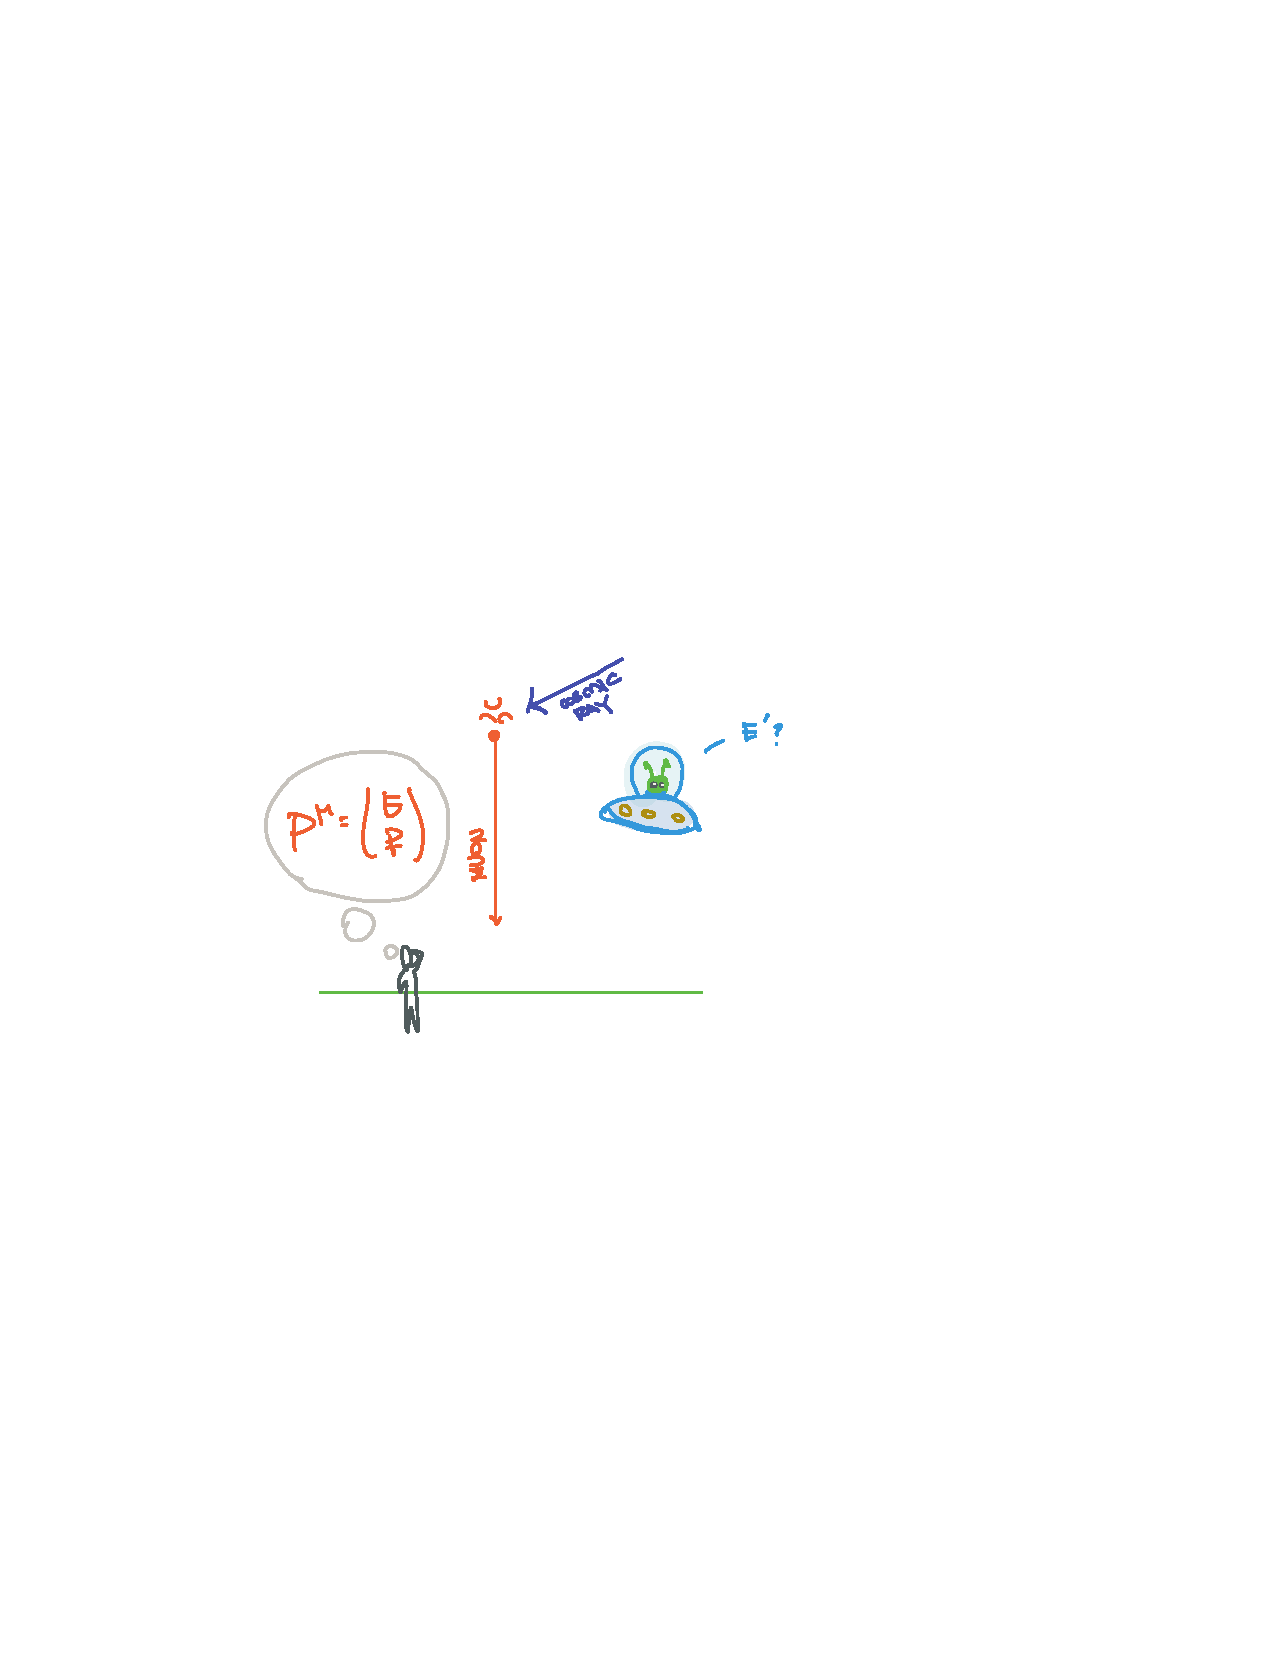
\includegraphics[width=\textwidth]{figures/alien.pdf}
    \captionsetup{font={scriptsize,sf}}
    \caption{You measure the four-momentum of a particle. What is the energy that an alien moving at some velocity $\beta$ relative to you measures?\label{fig:alien}}
\end{marginfigure}

At this point you wonder if we are simply reciting random facts that we have developed. Consider the following scenario illustrated in Fig.~\ref{fig:alien}.
%
% 
While you are measuring the particle energy $p^0 = E$, you notice an alien traveling relativistically with velocity $\beta$ relative to you. The alien has sophisticated equipment to measure the particle energy, and you know that the alien measures a different energy $E'$. How can you determine what the alien measures?

One way to do this is to calculate the full Lorentz transformation between your frame and the alien frame. That is tedious. It turns out that we can use the four-velocity as a useful trick. All objects with mass have a four-velocity equal to \eqref{eq:4:velocity:in:rest:Frame} in their rest frame. This means that the alien measures the particle to have energy $v_\text{alien}\cdot p_\text{alien}$, where the subscript `alien' means that these are all calculated in the alien's frame.

We now remember that $v_\text{alien}\cdot p_\text{alien}$ is a number. It does not matter what frame we calculate it in. Thus it is equivalent to the same dot product measured in our frame:
\begin{align}
E'=
    v_\text{alien}\cdot p_\text{alien} = v\cdot p \ ,
\end{align}
where the right-hand side is the alien four-velocity and the particle four-momentum as measured in our frame. The alien four-velocity is simply a Lorentz transformation of \eqref{eq:4:velocity:in:rest:Frame}. More practically, it is something that you can measure in your own frame. 


\begin{exercise}
Rephrase everything in this example in terms of the inner product in Minkowski space. Bonus if you use the word `projection.'
\end{exercise}






\section{Tensors: the meaning of indices}


The lightning-quick review of special relativity here is an example of tensor analysis in physics.\sidenote{Where can you learn more? I recommend my Physics 17 lecture notes. Want a more advanced version? Check out my Physics 231 lecture notes.} Tensors show up \emph{all over the place} in physics. Even in your lower division physics courses: did you ever wonder why it is called the moment of inertia \emph{tensor} and not the moment of inertia \emph{matrix}? Yes, there is a difference.\footnote{See e.g.\,\url{https://hepweb.ucsd.edu/ph110b/110b_notes/node24.html}}\sidenote{I am frustrated that few textbooks take a moment to explain the significance this difference.} For our purposes, we can think of a \textbf{tensor}\index{tensor} as an object that has an ordered number of indices. The indices each have a height, either upper or lower. 

The order of the indices matters; if you want it takes precedence over the height of the index: 
\begin{align}
    T^{ij\phantom{k}\ell}_{\phantom{ij}k} \neq
    T^{\phantom{k}ij\ell}_{k} \ .
\end{align}
If you have a metric, this is more clear since you can lower (or raise) all the indices, so that 
\begin{align}
    T^{ij\phantom{k}\ell}_{\phantom{ij}k} &= T^{ijm\ell}g_{mk}
    \\
    T^{\phantom{k}ij\ell}_{k}&=T^{mij\ell} g_{mk}
\end{align}
and you can see that $T^{mij\ell} \neq T^{ijm\ell}$.

There are some equivalent ways of thinking about tensors. The most formally correct way is to think about them as \emph{multilinear maps} between vector spaces (or tensor products\sidenote{Given a vector space $V$, a tensor product $V\otimes V$ is two copies of the vector space.} thereof). Perhaps more practically, a tensor is an object that encodes information that transforms according to the height of the indices. Generalizing our rules from Section~\ref{sec:Lorentz:transformations}:
% 
\begin{newrule}[Tensor transformation]\label{rule:tensor:transform}
If $T$ is a tensor with upper indices $i_1, \cdots, i_N$ and lower indices $j_1, \cdots, j_M$, then under a symmetry transformation $R(\theta)$, $T$ transforms as
\begin{align}
    T^{\cdots}_{\cdots} \to 
    R(\theta)^{i_1}_{\phantom{i_1} k_1} 
    \cdots 
    R(\theta)^{i_N}_{\phantom{i_N} k_N}
    (R(\theta)^{-1})^{\ell_1}_{\phantom{\ell_1}j_1} 
    \cdots 
    (R(\theta)^{-1})^{\ell_M}_{\phantom{\ell_M}j_M} T^{\cdots}_{\cdots} \ ,
\end{align}
where we have written $\cdots$ on the left hand side to mean `some arrangement of upper $i$ and lower $j$ indices,' while on the right the $\cdots$ mean `some arrangement of upper $k$ and lower $\ell$ indices.'

In other words:
\begin{itemize}
    \item For each upper index, multiply by a factor of $R(\theta)$ and contract with the lower index of $R(\theta)$.
    \item For each lower index, multiply by a factor of $R(\theta)^{-1}$ and contract with the upper index of $R(\theta)^{-1}$. Note that this is contraction with the \emph{first} index of $R(\theta)^{-1}$. 
\end{itemize}
\end{newrule}
To apply the rule for Lorentz transformations, simply replace $R$ with $\Lambda$ and convert the indices into $\mu$s and $\nu$s. 

We ultimately care about quantities that are \emph{invariant}\index{invariant} under Lorentz transformations. These are objects that everyone agrees upon, no matter what their reference frame. If you were to build a theory of nature, you would want the physical laws from that theory to be invariant with respect to reference frame---so the objects you would build that theory out of are naturally invariants. 





\section{Isometry}

How does one know that rotations are important symmetries in Euclidean space? This certainly comes from our own experience with physics---the laws of physics are rotationally invariant. In fact, we learn very quickly in our physics training to use rotational invariance to simplify problems. What about in special relativity? Historically, the Michelson--Morley non-observation\sidenote{Perhaps the most significant null result in science.} of aether---that is, the observation that the speed of light is constant---led us to realize that requirement that physics cannot depend on reference frame leads to a different class of symmetries. What characterizes these symmetries?

From a top-down perspective, rotations and their generalizations\sidenote{Such as Lorentz transformations in special relativity.} are \emph{isometries}. An \textbf{isometry} is a symmetry of \emph{the form of the metric}. Specifically, it is a transformation---enacted by a matrix acting on vectors, for example---for which the \emph{components} of the metric do not change. With our conventions, special relativity requires that the components of the metric are $\eta_{\mu\nu} = \text{diag}(+,-,-,-)$; this means that the metric takes this form in \emph{any} reference frame. 

Ah! But we know from Rule~\ref{rule:tensor:transform} that the metric is an object with two lower indices. That means that it has a prescribed transformation rule. If $v^\mu \ to R\aij{\mu}{\alpha}v^\alpha$ for some transformation $R$, then the metric transforms as
\begin{align}
  g_{\mu\nu} \to   R\aij{\alpha}{\mu} R\aij{\beta}{\nu} g_{\alpha\beta} \stackrel{?}{=} g_{\mu\nu} \ .
\end{align}
For $R$ to be an isometry, the last expression (marked `?') must be true:
\begin{align}
    R\aij{\alpha}{\mu} R\aij{\beta}{\nu} g_{\alpha\beta} = g_{\mu\nu} \ .
    \label{eq:defining:isometry}
\end{align}
We call the isometries of spacetime Lorentz transformations\index{Lorentz transformation} and typically write $R=\Lambda$. The isometries of Euclidean space are the rotations, which we usually keep writing as $R$. In this course we also meet the complex versions of rotations,\sidenote{This should familiar from quantum mechanics. Symmetries are described by a mathematical class called a group. Rotations in $N$ dimensions are the group $\textnormal{SO}(N)$ for ``special orthogonal'' $N\times N$ matrices. Special means unit determinant and orthogonal means $R^\trans R = \one$. The complex version is the group $\textnormal{SU}(N)$, for special \emph{unitary} matrices. Unitary means $U^\dag U = 1$.} which we write $R=U$.

\begin{exercise}[Definition of Lorentz Tranform]
\label{ex:lorentz:definition:indices}
The relation \eqref{eq:defining:isometry} in special relativity is
\begin{align}
    \Lambda\aij{\alpha}{\mu} \Lambda\aij{\beta}{\nu} \eta_{\alpha\beta} = \eta_{\mu\nu} \ .
\end{align}
This is of course just a change of symbols. When this is introduced in some textbooks, they often write it in matrix form rather than index form:
\begin{align}
    \Lambda^\trans \eta \Lambda = \eta \ .
\end{align}
Show that these two forms are indeed equivalent. \textsc{Hint}: the matrix formalism suppresses indices because it assumes that consecutive indices are contracted. 
\end{exercise}
% 
\begin{example}
In Exercise~\ref{ex:lorentz:definition:indices}, you were faced with something that is rarely explained: if a matrix has indices $M\aij{i}{j}$, what is the index structure of the transpose, $M^\trans$? More generally, given a linear transformation $M$, what is the index structure of the \emph{adjoint}, $M^\dag$? 

Exercise~\ref{ex:lorentz:definition:indices} gives you a hint for this. The correct identification is
\begin{align}
    {M^\dag}\aij{i}{j} = M\aij{j}{i} \ ,
\end{align}
but this does not seem to make sense because the heights of the indices do not match. In fact, what we really mean is
\begin{align}
    {M^\dag}\aij{i}{j} = g_{\ell j} g^{ki} A\aij{\ell}{k} \ .
    \label{eq:def:adjoint}
\end{align}
The way to see this is to go from the root definition of the adjoint with respect to the inner product. Recall that the inner product is a (bi-)linear function that takes two vectors and returns a number. It is defined with respect to the metric as
\begin{align}
    \la \vec{v}, \vec{w} \ra = g_{ij}v^iw^j \ .
\end{align}
Then the adjoint $M^\dag$ is defined relative to $M$ to be the matrix that satisfies
\begin{align}
    \la \vec{v}, M^\dag \vec{w} \ra = 
    \la M \vec{v}, \vec{w} \ra
\end{align}
for every choice of $\vec{v}$ and $\vec{w}$. Writing out this expression with explicit indices gives
\begin{align}
    g_{ab} v^a {M^\dag}\aij{b}{c} w^c
    &= 
    g_{de} M\aij{d}{f}v^f w^e 
    \ .
\end{align}
Observe that all indices are contracted---they are all dummy indices and can be relabeled for convenience. Let us do this for the right-hand side so that the indices on $\vec{v}$ and $\vec{w}$ match those on the left-hand side:
\begin{align}
    % g_{ab} \cancel{v^a} {M^\dag}\aij{b}{c} \cancel{w^c}
    % &= 
    % g_{dc} M\aij{d}{a} \cancel{v^a} \cancel{w^c}
    g_{ab} {v^a} {M^\dag}\aij{b}{c} {w^c}
    &= 
    g_{dc} M\aij{d}{a} {v^a} {w^c}
    \ .
\end{align}
Usually one avoids repeating the use of indices since this can lead to ambiguities about which indices are contracting; here there is no such issue because each side of the equal sign is evaluated independently. \emph{However}, we make a clever observation: the equality holds for \emph{any} vectors $\vec{v}$ and $\vec{w}$. This means we can choose basis vectors where only the $a^\textnormal{th}$ component of $\vec{v}$ and the $c^\textnormal{th}$ component of $\vec{w}$ are non-zero---for any specific choice of $a = \hat{a}$ and $c = \hat c$. In that case, the sum over these dummy variables collapses to those specific choices of hatted index:
\begin{align}
    g_{\hat ab} {v^{\hat a}} {M^\dag}\aij{b}{\hat c} {w^{\hat c}}
    &= 
    g_{d\hat c} M\aij{d}{\hat a} {v^{\hat a}} {w^{\hat c}}
    &&
    \text{no sum over hatted indices}
    \\
    g_{\hat ab} \cancel{v^{\hat a}} {M^\dag}\aij{b}{\hat c} \cancel{w^{\hat c}}
    &= 
    g_{d\hat c} M\aij{d}{\hat a} \cancel{v^{\hat a}} \cancel{w^{\hat c}}
    &&
    \text{no sum over hatted indices}
    \\
    g_{\hat ab} {M^\dag}\aij{b}{\hat c} 
    &= 
    g_{d\hat c} M\aij{d}{\hat a} 
    &&
    \ .
\end{align}
Because there was no sum over hatted indices, we can cancel out the common factor of $v^{\hat a}w^{\hat c}$ on both sides.  The last line gives \eqref{eq:def:adjoint} upon contracting with the inverse metric $g^{\hat a e}$ on both sides and then re-naming the indices appropriately.\footnotemark
\end{example}\footnotetext{See also \url{https://threadreaderapp.com/thread/1702863061047263428}}
% 

\begin{example}
Let us also clarify the phrase \emph{the components of the metric are unchanged} as related to isometries. This is different from saying \emph{the inner product is preserved}. For any transformation---not necessarily an isomsetry---$\vec{v}\to A\vec{v}$, the inner product is preserved \emph{if you also allow the metric to transform}:
\begin{align}
    \la \vec{v}, \vec{w}\ra
    = 
    g_{ij}v^i w^j
    &\to 
    {A\inv}\aij{k}{i}\, {A\inv}\aij{\ell}{j}
    g_{ij}
    \,
    A\aij{i}{m} v^m \, A\aij{j}{n}v^j
    \\
    &= ({A\inv} A)\aij{k}{m} ({A\inv} A)\aij{\ell}{n} g_{k\ell} v^m w^n
    \\
    &= g_{k\ell} v^k w^\ell 
    =\la \vec{v},\vec{w} \ra
    \ .
\end{align}
The point though, is that we do \emph{not} let the metric transform. A transformation where the metric transforms cannot be interpreted as a chance of reference frame since all reference frames are supposed to see the same components of the metric. 

This is obvious when considering transformations like $A = \textnormal{diag}(3,3)$. This stretches the length of vectors by a factor of 3. This is only meaningful as a physical transformation if we do not simultaneously transform the metric.
\end{example}


\begin{example}
It is clear that rotations (Lorentz transformations) are a leave the metric unchanged. What about translations? We know that translation invariance is a symmetry of spacetime---the homogeneity of space leads to momentum conservation. Why do we not have a matrix $R$ for translations?

This is related to the point in Section~\ref{sec:index:upper} that there is no such thing as a `position vector' and the definition of \emph{linear} in \eqref{eq:def:linear:oneform}. There is simply no such thing as translation in a vector space. In a vector space, the origin means something: it is the null (zero) vector. Translations do not make sense because they say that a different element is now the null vector. This makes no sense because the null vector is the unique element for which $\vec{0}+\vec{v} = \vec{v} + \vec{0} = \vec{v}$ for any $\vec{v}$. 

Of course, translations \emph{are} a key part of understanding physics. Vector spaces are just the wrong structure to describe them. The vector spaces that we deal with for spacetime are \textbf{tangent planes} to spacetime. A particle's velocity $\vec{v}$ is a vector of a tangent plane at a point $p$ on spacetime. We say that
\begin{align}
    v\in \textnormal{T}_p{M} \ ,
\end{align}
which means the tangent plane at point $p$ on the spacetime (manifold) $M$. At a different point, $p'$, the particle's velocity is part of a different tangent plane, $\textnormal{T}_{p'}M$. Imagine the spaces of tangent vectors at some point on the equator versus at the north pole. Both of these are two dimensional vector spaces embedded in tree-dimensional ambient space. But these two dimensional planes are quite different. You cannot place a generic vector from one space onto the other space. \flip{Insert picture}

All this is to say that the mathematical structure for including spacetime translations is different from the structure of a vector spaces. In fact, it is the collection of each vector space over each point in the spacetime. This collection is called $\textnormal{T}M$, the \textbf{tangent bundle}\index{tangent bundle} over the spacetime $M$. 

By way of analogy: the metric is implicitly present in Euclidean space, but it is so trivial that we do not even define it when we first learn about vectors. In the same way, the tangent bundle is a structure that is implicitly present in special relativity but is so trivial---every tangent space looks like every other tangent space---that we never bring it up. However, in general relativity, the tangent bundle comes to life. In the example of the tangent spaces at the equator versus the north pole: because the underlying space has \emph{curvature}, the ways in which tangent spaces are related to one another is no longer trivial. The curvature of spacetime---gravity---is mathematically understood to be a change in the relationships of tangent spaces. Because tangent spaces are where velocities live, this picture gives you an idea of how velocities may change (accelerate) in the presence of gravity.

To push this further: you also appreciate that there are other forces in nature---say, electromagnetism---that can accelerate test particles. Can these also be understood as some kind of tangent bundle? Yes! This is the mathematical structure of \emph{gauge theory} and is the framework for what we call the fundamental forces. In this way, curvature in `internal spaces' (not spacetime) is the origin of the fundamental forces in particle physics. The mathematical structure is precisely the same as that of gravity. In general, both gravity and the fundamental forces of particle physics are gauge theories; all of these forces are understood as tangent bundles over spacetime. 

For a good starting point for all of this, I recommend the lecture notes by Collinucci and Wijns: \cite{Collinucci:2006hx}.
\end{example}

\begin{subappendices}

\section{Relativity by Thought Experiment}\label{sec:subappendix:relativity}
You can derive special relativity from the assumption that the speed of light is constant in any reference frame and then doing so called \emph{gedankenexperiments}.\sidenote{`Thought experiments' in German.} We continue our convention of using natural units where $c=1$, though it should be obvious that using any other units just throws in factors of $c$ all over the place.
\begin{exercise}
Rewrite all the equations in this appendix with the appropriate factors of $c$. Stop when it becomes obvious how to do this. 
\end{exercise}
I first saw this done in Chapter 15 of \emph{The Feynman Lectures on Physics}\footnote{\url{https://www.feynmanlectures.caltech.edu/I_15.html}}\sidenote{\emph{The Feynman Lectures on Physics} are beloved gems of freshman-level physics insight---but the consensus is largely that they are a bit too non-sequitur in style for physics students. In fact, you come to deeply enjoy the lectures only \emph{after} you already understand most of the material---then you can appreciate the little brilliant twists that Feynman makes compared to the usual pedagogy.} I refer you to that resource for a systematic derivation from the \emph{gedanken} approach. In this appendix, follow the the general idea and focus on a few subtle points that are not often explained carefully in the standard literature.\sidenote{I thank Matthew Lugatiman and Adam Green for talking through some of these subtleties with me.}

Just as the word \emph{gedankenexperiment} tells you where special relativity was developed, so too does the standard setting of the \emph{gedankenexperiment}: start by imagining a train moving with some velocity $v=\beta$ in the $x$ direction relative to our coordinate system. We are \emph{outside} the train. We are observers, $\mathcal O$ and our coordinate system is $(t,x)$. You can also imagine another observer, Oppie,\sidenote{This is \emph{not} a reference to Oppenheimer's nickname or a misspelling of Opie, Ron Howard's most famous character. Instead, it's a name that is reasonably close to $\mathcal O'$, ``oh-prime.''} who is \emph{in} the train and whose coordinate system carries primes: $(t',x')$. We say that Oppie is a \emph{comoving} observer with the train. We align our coordinate systems so that the origins coincide: 
\begin{align}
    (t=0,x=0) = (t'=0,x'=0) \ .
\end{align}
The above equation should be treated to mean \emph{the point that we call $(0,0)$ coincides with the point that Oppie calls $(0,0)$.} In this way, a generic point $(t,x)$ is really a \emph{separation} between that point and the origin.\sidenote{Recall our caveat in Chapter~\ref{sec:index:upper}: positions are not vectors, but differences in positions are vectors.}


\subsection{Time dilation}

First imagine that Oppie has a little gizmo that first emits a photon towards a mirror, then detects the reflected photon. See Fig.~\ref{fig:Feynman:photo:thing}
\begin{marginfigure}%[th]
    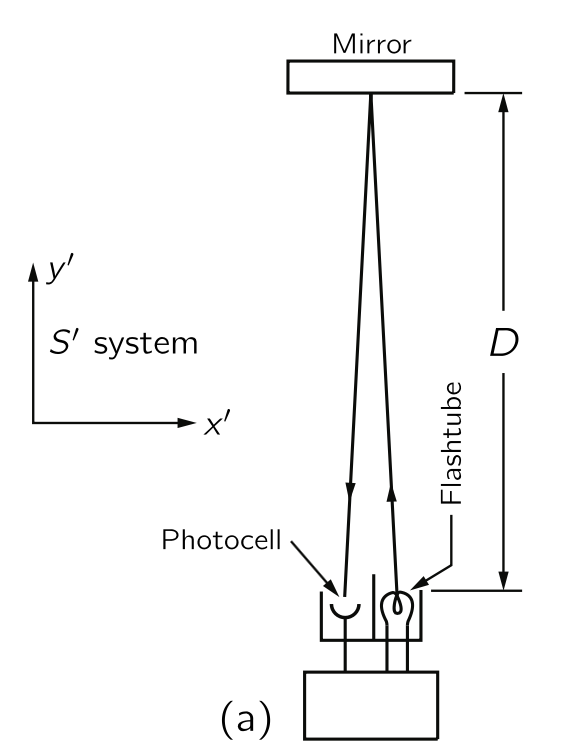
\includegraphics[width=.8\textwidth]{figures/FeynmanLec15_photodet.png}
    \captionsetup{font={scriptsize,sf}}
    \caption{From \emph{The Feynman Lectures on Physics}, Chapter 15.}
    \label{fig:Feynman:photo:thing}
\end{marginfigure}
The height of the gizmo is $D = \ell$, the height of the train. It is critical that the gizmo is aligned so that the photon moves \emph{perpendicular} to the direction of motion. We write $\ell$ for \emph{length} and to avoid ambiguities with [covariant] derivatives, $D$ mesons, and so forth. 

Like us, Oppie understands that the speed of light is $c=1$ and that this is true in any reference frame. At the origin ($t'=0$), Oppie turns ont he gizmo and measures the time $t'$ that it takes for the photon to traverse the distance $\ell$ and come back. 
\begin{align}
     t' = 2\ell/c = 2\ell \ .
     \label{eq:Feynman:train:updown}
\end{align}

What do we see? Like Oppie, we see the device turn on at the origin ($t=0$) and we see that the photon hits the roof of the train car and bounces back down. However, unlike Oppie, we also see the entire system move in direction of the train's motion. The trajectory is shown in Fig.~\ref{fig:Feynman:photo:thing:unprimed}.
\begin{figure}[ht]
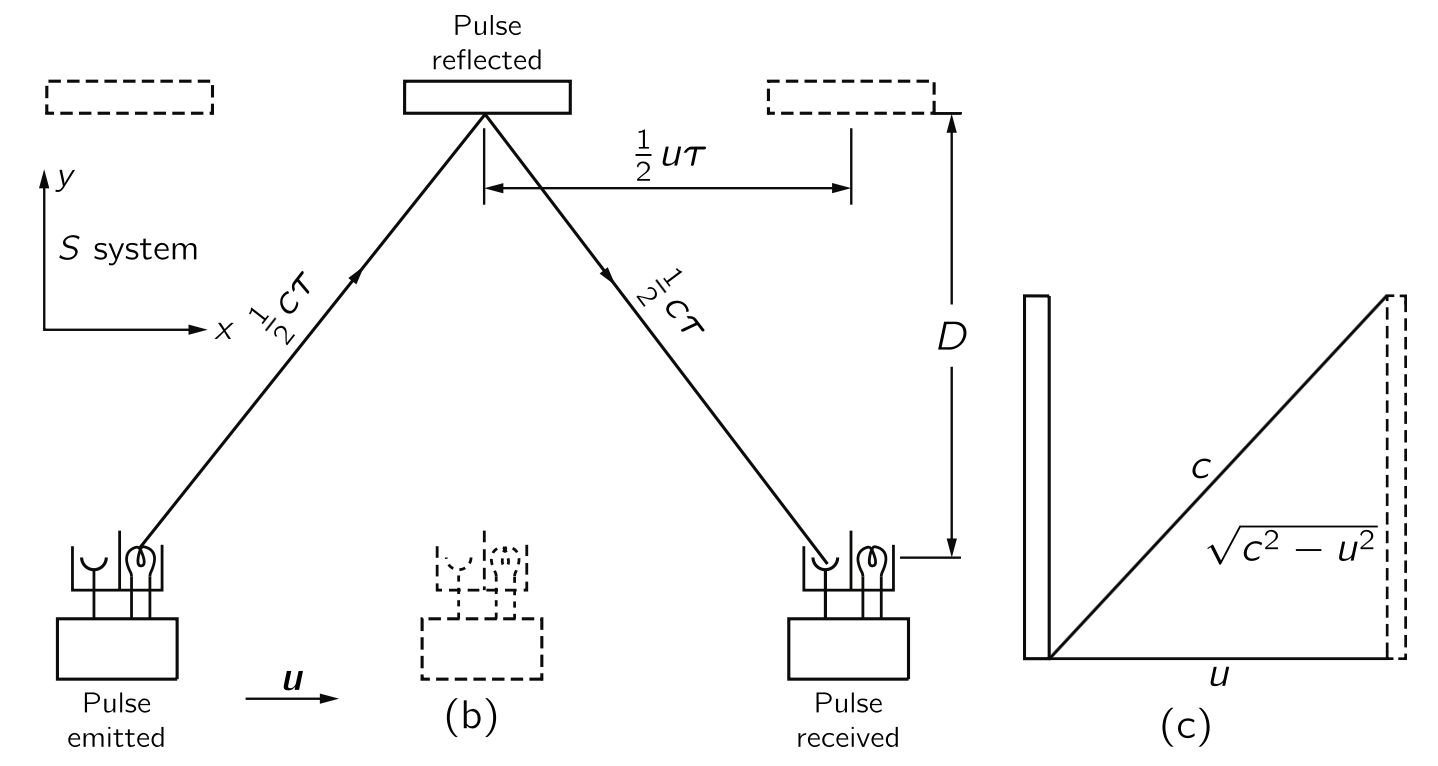
\includegraphics[width=\textwidth]{FeynmanLec15_photodetside.png}
    \captionsetup{font={scriptsize,sf}}
    % \caption
    \sidecaption[][-7em]{Same as Fig.~\ref{fig:Feynman:photo:thing}, but as seen from observers who are not on the train. From \emph{The Feynman Lectures on Physics}, Chapter 15.
    \label{fig:Feynman:photo:thing:unprimed}
    }
\end{figure}
Because the motion of the train is perpendicular to the up-and-down direction, we assume that the height of the train is unchanged by relativistic effects: we measure this height to be $\ell$ just as Oppie does. We then measure that the photon takes times $t$ to hit the top of the train and return. This time is evenly split\sidenote{By symmetry.} between the upward-going time and downward-going time. During this time, the train has moved along the $x$ direction by an amount $\beta t$. From trigonometry, we thus have:
\begin{align}
    \left(\frac{t}{2}\right)^2
    &= 
    \left(\frac{\beta t}{2}\right)^2 + \ell^2
\end{align}
Plugging in Oppie's observation that that relates the height of the train to the time Oppie measures, \eqref{eq:Feynman:train:updown}, we have
\begin{align}
    (t')^2 = (1-\beta^2) t^2 =  \frac{t}{\gamma} \ .
\end{align}
That is to say, the time that we measure is related to the time that Oppie measures by
\begin{align}
    t = \gamma t' \ .
    \label{eq:time:dilation:derived}
\end{align}
Because $\gamma > 1$, we the time that we see is \emph{dilated} relative to what Oppie experiences. Because the gizmo is essentially an idealized clock, we say that observers see the events on the moving train moving  slower than they would expect by a factor $\gamma$. 




\subsection{Length contraction}

Having learned something about the passage of time, we can now figure out what motion does to the relative perception of space. To do this, let us do a second experiment where we turn the gizmo in Fig.~\ref{fig:Feynman:photo:thing} onto its side. Place the gizmo at the back of a train car and arrange it so that the photon first moves \emph{along the direction of the train's motion}, then reflects off of the mirror to go \emph{against the direction of the train for its return motion}. Let us now set the length of the gizmo to be the length of the train car: Ollie observes\sidenote{We write $\ell_0$ rather than $\ell'$ because Ollie is in the rest frame of the train. $\ell_0$ is called a \emph{proper length}, it is the length of an object to an observer for whom the object is not moving.} this to be $\ell_0$ while we observe it to be $\ell$. 

In pre-special relativity Galilean physics we would expect $\ell_0 = \ell$. However, the fact that $c=1$ is constant means that we cannot make this assumption. 
\begin{marginfigure}%[th]
    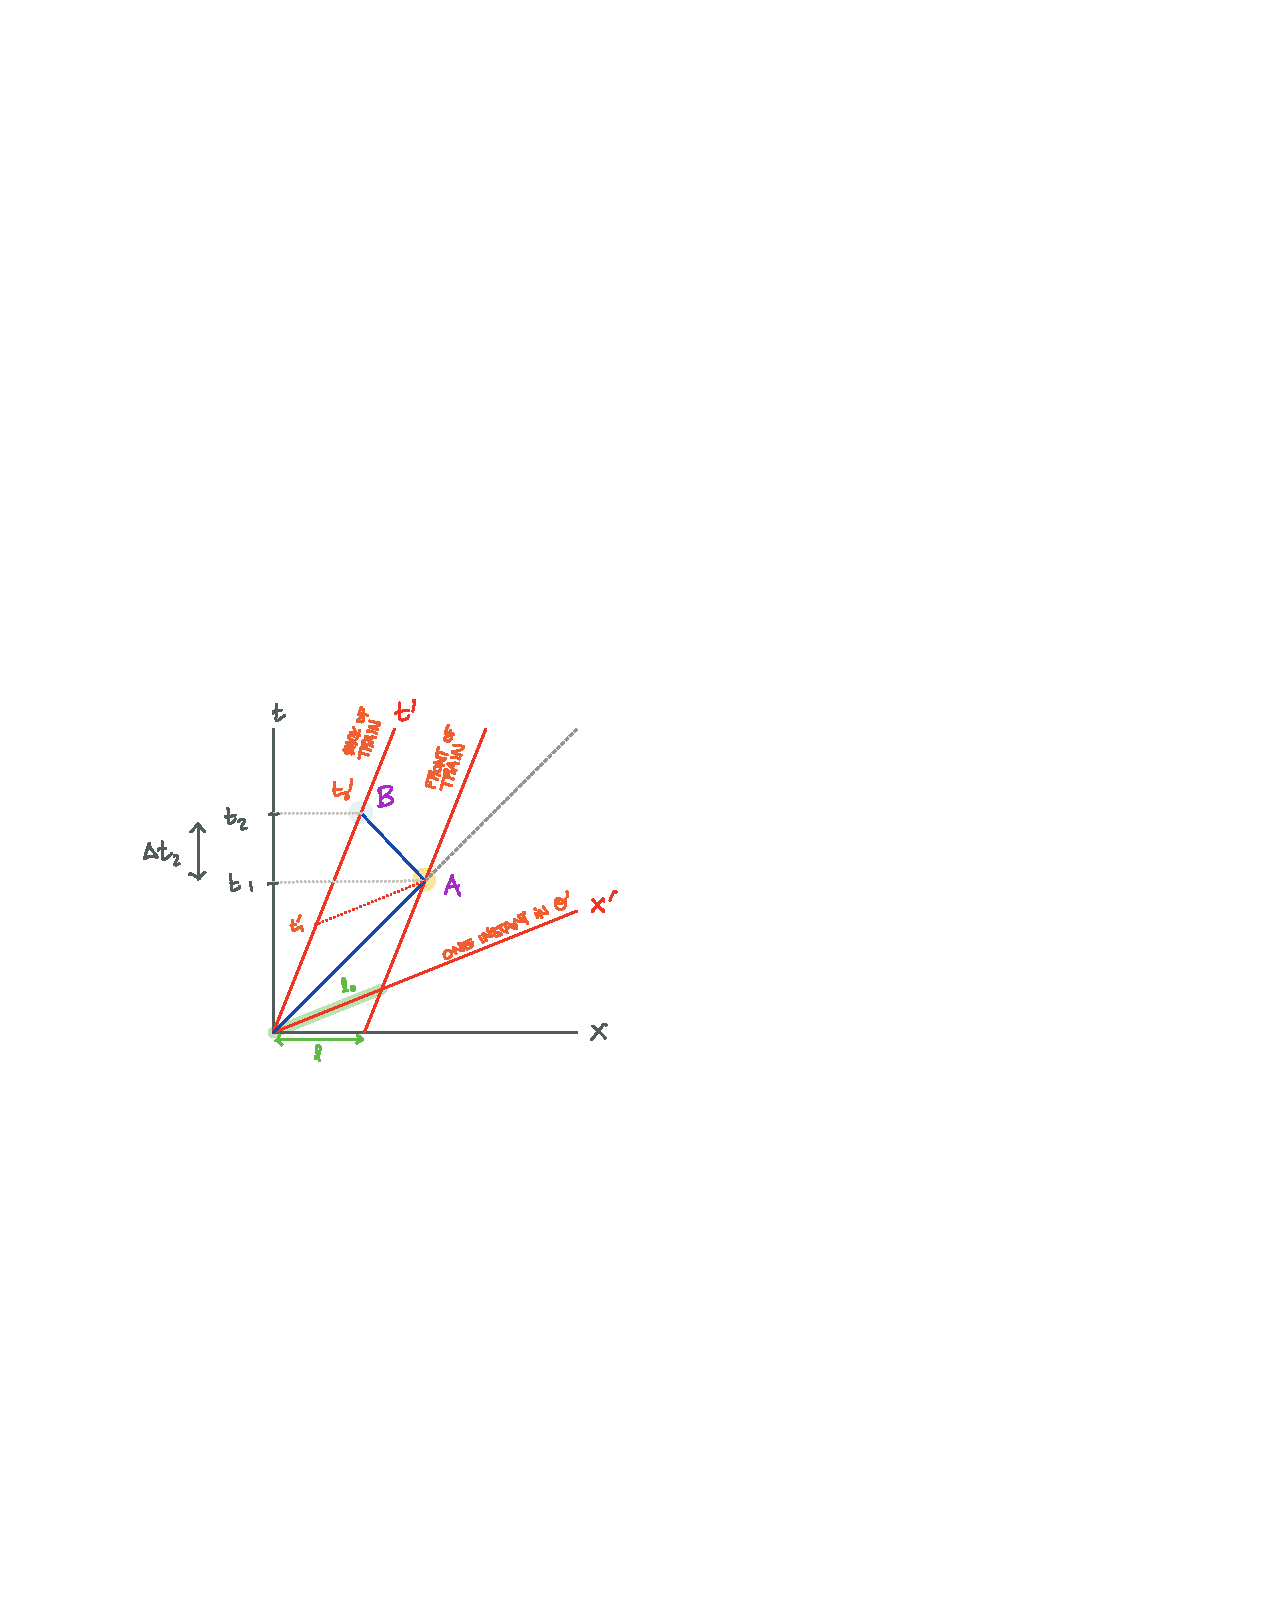
\includegraphics[width=\textwidth]{figures/spacetime_lengthcontraction.pdf}
    \captionsetup{font={scriptsize,sf}}
    \caption{The trajectory of the photon (dark blue) from the back of the train at $t=t'=0$ to the event $A$ then the event $B$ where it returns to the back of the train. Oppie's coordinate system is in red. \label{fig:spacetime:length:diagram}}
\end{marginfigure}
Points on a spacetime diagram are called \emph{events} because they are a place and a time. Figure~\ref{fig:spacetime:length:diagram} shows the experiment. Let the origin be the back of the train at time zero---where both we and Oppie synchronize our clocks. A photon is shot towards the end of the train. The two edge of the train correspond to the $t'$ axis and its parallel translation---this is because in Oppie's frame the train is not moving and so it stays at $x'=0$; similarly, the front of the strain stays at $x'=\ell_0$. 

The photon travels at the speed of light $c=1$, which is a 45$^\circ$ diagonal line on the way out, then a 135$^\circ$ line on the way back. The thought experiment is again simpler in Oppie's frame. Oppie measures that the total time for the back-and-forth journey is $t_2' = 2\ell'$. It is clear both from the thought experiment and the diagram that each leg of the journey takes the same amount of time $t_2' = 2t_1'$.

We see something a bit different. On the outbound journey the photon has to \emph{catch up} to the front train. If we could observe it, we would measure that it takes time $t_1$ for the photon to reach the mirror. After it reflects off the mirror at the front of the train, the photon and the back of the train are moving \emph{toward each other}. We observe that this total journey takes a time $t_2$. We also define $\Delta t_2 = t_2 - t_1$ to be just the time of the journey from the front of the train to the back again. Observe that $\Delta t_2 \neq t_1$; both logically and from Figure~\ref{fig:spacetime:length:diagram}. This means we have the relations:
\begin{align}
t_1 &= \ell + \beta t_1
&
\Delta t_2 &= \ell - \beta \Delta t_2 \ .
\end{align}
Here we recall that $\beta$ is the speed of the train and the different signs correspond to whether the train is moving with or against the photon. Since $t_1$ is already measured against the origin, there is no need to write $\Delta t_1 \equiv t_1 - 0 = t_1$. These give us the relations:
\begin{align}
    (1-\beta)t_1 &= \ell & (1+\beta)\Delta t_2 &= \ell
    \ .
\end{align}
The total time is then
\begin{align}
    t_2 = t_1 + \Delta t_2 = \frac{\left[(1 + \beta) + (1-\beta)\right]\ell}{1-\beta^2}
    = 2\gamma^2 \ell \ .
    \label{eq:gedanken:length:intermediate1}
\end{align}
\begin{exercise}
Prove \eqref{eq:gedanken:length:intermediate1}. It is worth doing.
\end{exercise}
Now we have to invoke time dilation in \eqref{eq:time:dilation:derived}. The total time for the round trip journey that we measure $t_2$ is related to the total time that Oppie measures $t_2'$ by
\begin{align}
    t_2 &= \gamma t_2'
    \\
    2\gamma^2 \ell &= 2\ell' 
    \\
    \ell = \frac{\ell'}{\gamma}
    \label{eq:length:contraction:derived}
    \ .
\end{align}
Because $\gamma > 1$, we find that what \emph{we} measure to be the length of the train is \emph{contracted} (smaller) relative to what Oppie measures in the comoving frame of the train.


\subsection{Confusion}

The lessons of this \emph{gedanken} appendix are simple. If the frame $\mathcal O'$ is moving relative to our frame, $\mathcal O$, then
\begin{itemize}
    \item From \eqref{eq:time:dilation:derived}: The time that we measure is \emph{dilated} (slower) compared to the time that is measured in $\mathcal O'$. 
    \item From \eqref{eq:length:contraction:derived}: Length along the direction of motion are \emph{contracted} (smaller) compared to the length along the direction of motion measured in $\mathcal O'$. 
\end{itemize}
Having established these, I leave it to you to explore some of the apparent paradoxes in special relativity such as the pole-in-barn paradox and the twin paradox. The spacetime diagrams that we draw are useful guides. As a hint, often the resolution to paradoxes is the observation that simultaneity is a frame-dependent notion.\sidenote{This has a manifestation for us: the locality of the fundamental interactions is a logical consequence of requiring causality in our theory. Interactions must happen at a single \emph{event} rather than over a finite separation in order for there to be a clear \emph{cause} that precedes an \emph{effect} in any valid reference frame.}

Thus far, everything we have discussed in this appendix is standard fare in a decent treatment of first-year modern physics. Let us focus on some of the conceptual hiccups that are not always explained carefully.

\paragraph{Could we derive length contraction without using time dilation?} You should feel unsatisfied. In relativity, space and time have equal footing. However, \emph{every} thought-experiment based derivation of special relativity starts by deriving time dilation and \emph{then} uses that result to derive length contraction. The reason for this asymmetry is that the time dilation thought experiment did not depend on the directions perpendicular to the train's motion: both the $\mathcal O$ and $\mathcal O'$ frame measured the height of the train to be $\ell$. On the other hand, the length contraction thought experiment had both spatial displacement $\ell$ \emph{and} a time displacement $t_2$ that needed to be measured in each reference frame. To say it differently: the time dilation experiment allowed us to ignore part of the spatial configuration. However, in the length contraction experiment you \emph{cannot} ignore the time separation because all experiments evolve in time.\sidenote{Philosophically: we perceive the universe as a sequence in time. We can imagine experiences where we are stationary in space, but we have no experiment---\emph{gedanken} or otherwise---where we are stationary in time.} Rest assured, the geometry \emph{does} respect the symmetry between space and time.

\paragraph{If they are so useful, why did we not draw a spacetime diagram for the time dilation experiment?} The time dilation experiment made use of a third dimension of spacetime, the height of the train. It is a bit of a pain to draw, and you still end up drawing the same right triangles in Fig.~\ref{fig:Feynman:photo:thing:unprimed}


\paragraph{Was it necessary for the photon to complete a full loop?} In these thought experiments, the the photon is emitted and detected by the same device: the trajectory is an `out and back' in runners parlance. For the time dilation experiment, it is obviously sufficient to consider only the trajectory from the origin to the ceiling. What about for the length contraction experiment? This is also possible. 
\begin{exercise}
Derive time dilation using the same thought experiment, but without the `return journey' to the back of the train. 
\end{exercise}
That this is possible is obvious for those with experience with relativity. However, it is useful pedagogically to have the photon perform a round trip journey because this way all observations are performed by the same observer. I can say that \emph{Oppie} emits a photon and \emph{Oppie} observes its return. Then we can identify the event where we observe Oppie emitting a photon and the event where we observe Oppie observing the photon.\sidenote{Given the subtleties of spacetime separated events with regard to simultaneity, I can appreciate this pedagogical choice.}

\paragraph{I tried calculating this using Lorentz transformations and I got stuck.} Here is a common error. Suppose we know that Oppie measures the train car to have length $\ell_0$ and that Oppie measures this at some time slice $t'=0$. Then we can perform a Lorentz transformation:
\begin{align}
    \begin{pmatrix}
        t\\
        \ell
    \end{pmatrix}
    =
    \begin{pmatrix}
        \gamma &\gamma\beta\\
        \gamma \beta & \gamma
    \end{pmatrix}
    \begin{pmatrix}
        0\\
        \ell_0
    \end{pmatrix}
    = 
    \begin{pmatrix}
        \gamma\beta\ell_0
        \gamma \ell_0
    \end{pmatrix} \ .
\end{align}
From this we believe that $\ell = \gamma \ell_0$, i.e.\ length is \emph{also} dilated---which is \emph{incorrect}! What went wrong here? Recall that the \emph{event} that we are using to measure the length of the train is a photon hitting the back of the train. That is labeled event $A$ in Fig.~\ref{fig:spacetime:length:diagram}. This occurs on the light cone where $t=x$ (and also $t'=x'$). That means that we need to Lorentz transform the separation between the \emph{event} $(t_1'=\ell_0, x'=\ell_0)$. This gives
\begin{align}
    \begin{pmatrix}
        t_1\\
        \ell
    \end{pmatrix}
    =
    \begin{pmatrix}
        \gamma &\gamma\beta\\
        \gamma \beta & \gamma
    \end{pmatrix}
    \begin{pmatrix}
        \ell_0\\
        \ell_0
    \end{pmatrix}
    = 
    \begin{pmatrix}
        \gamma(1+\beta)\ell_0\\
        \gamma(1+\beta)\ell_0
    \end{pmatrix} 
    \ .
\end{align}
We can use the first component and our time dilation result to find:
\begin{align}
    t_1 \equiv \ell &= \gamma (1+\beta)(1-\beta) \ell' 
    \\ &= \frac{\ell'}{\gamma}
    \ .
\end{align}
We have used the definition that $\gamma = (1-\beta^2)^{-1}$. 
From this we indeed confirm $\ell = \ell'/\gamma$ and that length is \emph{contracted}. 




\section{More examples in relativity}

\subsection{%Example: 
The electromagnetic field strength}
% motivate this from the unification of magnetism and electricity
% transformation laws

\begin{figure}[tb]
    \centering
    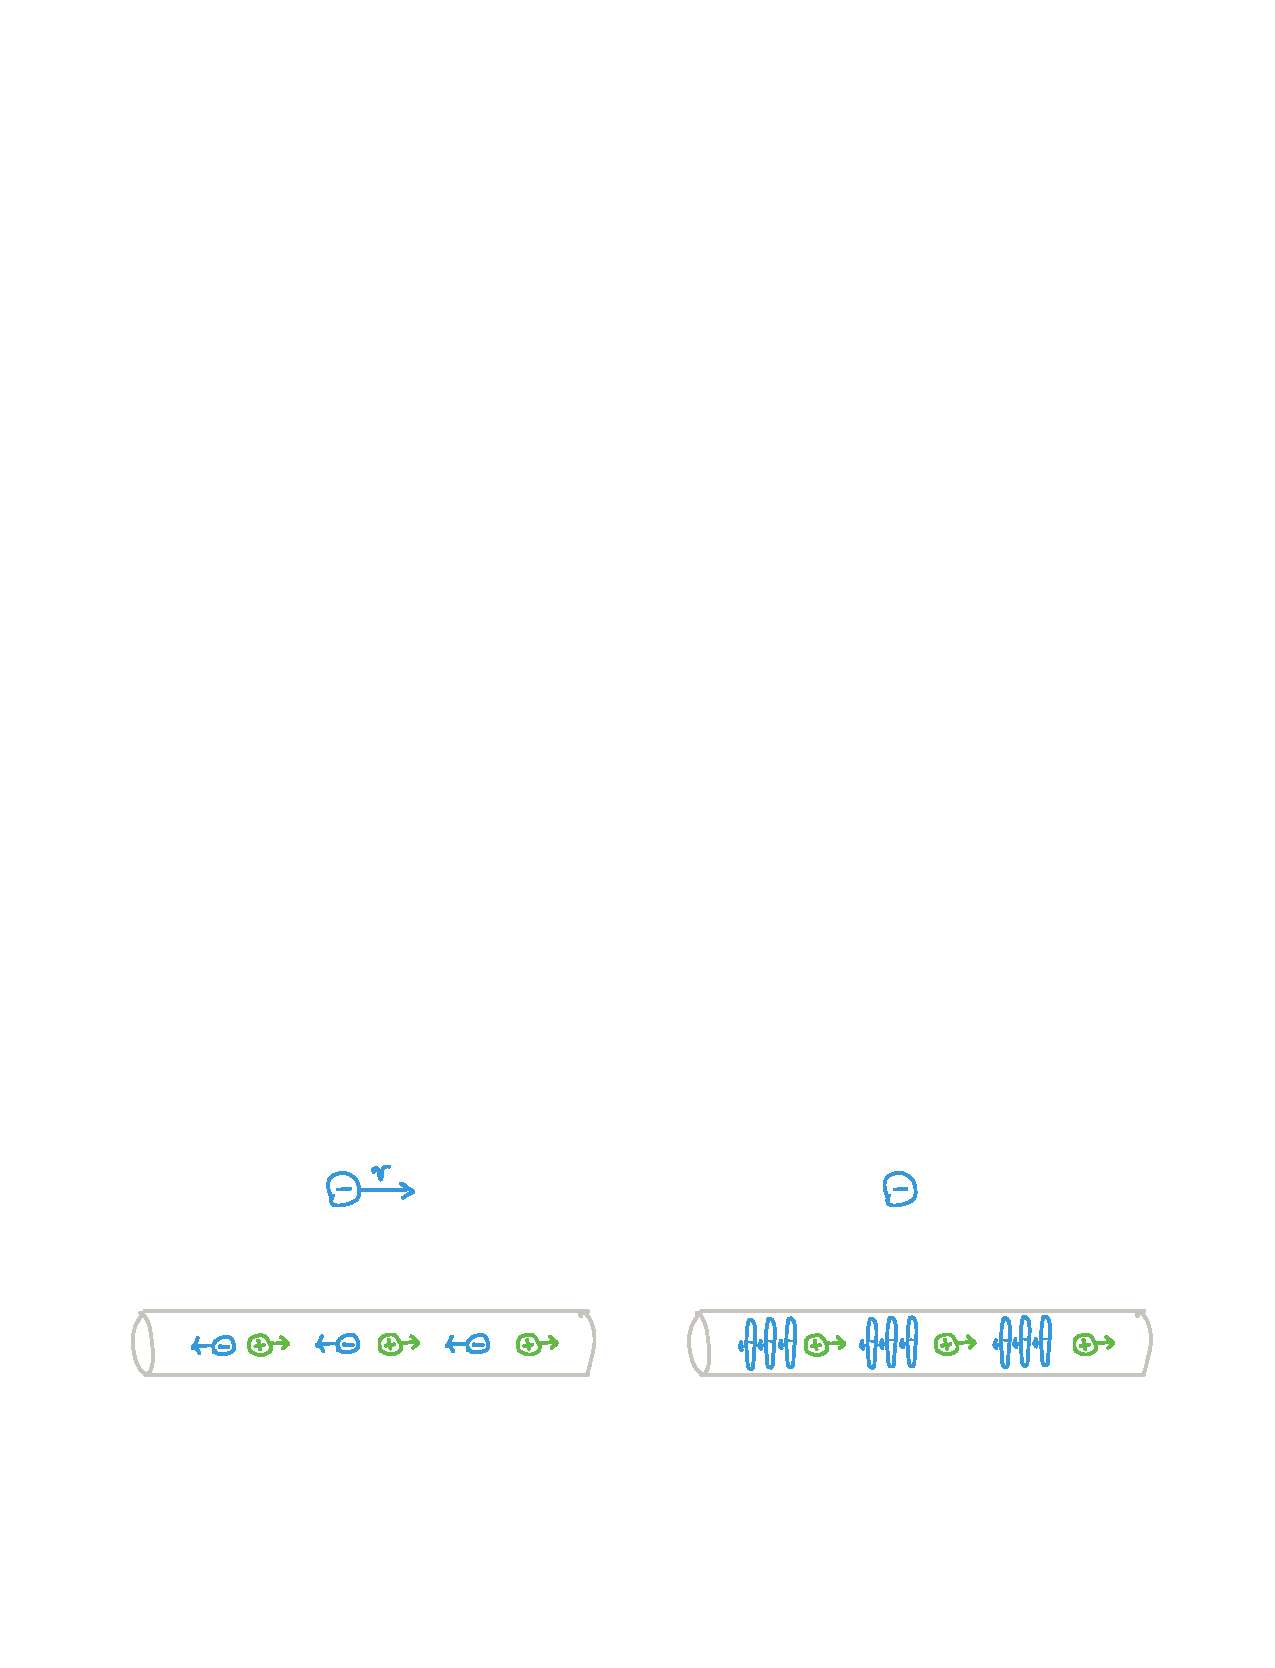
\includegraphics[width=\textwidth]{figures/EMcurrent.pdf}
    \caption{\textsc{Left}: an electron moves near a current. The current has no net electric charge. In the absence of magnetism, we expect the electron to move in a straight line. \textsc{Right}: if we boost into the electron frame, the particles in the current moving in the opposite direction are length-contracted. This means that the charge density increases. The stationary electron now feels a net electric force. This implies that something is missing in the picture on the left.}
    \label{fig:current}
\end{figure}

Another place where special relativity rears its head is in electrodynamics. Electricity and magnetism are two manifestations of the same electromagnetic phenomenon.\sidenote{Unification of apparently unrelated forces is a big theme of this course. Electromagnetism is the example that you already know.} This is illustrated in Fig.~\ref{fig:current}. If you did not know about magnetism, you would find a paradox when you consider a charged particle moving along a current. In one frame, the current is an equal number of positive and negative charges moving in opposite directions.\sidenote{I suppose more realistically the negative charges move while the positive charges stay put---that does not change the conclusion.} If you boost to the external charged particle's rest frame, length contraction forces one species of the current particles to increase their charge density relative to the other species. This creates a net electric field that acts on the stationary external particle. Without magnetism, the first frame is missing this additional force. 

The electric and magnetic fields are unified in the \emph{electromagnetic field strength}, which is a two-index tensor:
\begin{align}
    F^{\mu\nu}
    &=
    \begin{pmatrix}
        0&-E^x&-E^y&-E^z\\
        E^x&0&-B^z&B^y\\
        E^y&B^z&0&-B_x\\
        E^z&-B^y&B^x&0
    \end{pmatrix} %\ .
    &
    F_{\mu\nu}
    &=
    \begin{pmatrix}
        0&E^x&E^y&E^z\\
        -E^x&0&-B^z&B^y\\
        -E^y&B^z&0&-B_x\\
        -E^z&-B^y&B^x&0
    \end{pmatrix} \ .
\end{align}
We see that electricity and magnetism are unified in that their components mix into one another under a Lorentz transformation. 
\begin{exercise}
Confirm that $F_{\mu\nu} =g_{\mu \alpha}g_{\nu\beta} F^{\alpha\beta}$ with the (3+1)-dimensional Minkowski metric $g_{\mu\nu}$. 
\end{exercise}
\begin{exercise}
Find the components of $F'^{\mu\nu}$ under a boost along the $z$-direction. 
\end{exercise}


\subsection{%Example: 
Simultaneity}
\label{eq:simultaneity}

One of the key ideas in special relativity is that we sacrifice our notion of simultaneity for objects that are not observed at the same spacetime point. We may reuse our diagram in Fig.~\ref{fig:re:dilation}. Consider two different points on the $x'$ axis. These are simultaneous with respect to the primed observer: they both occur at $t'=9$. However, these two points  obviously do \emph{not} have the same $t$ coordinate to the unprimed observer. This observation helps clear up several apparent paradoxes that may show up in relativity. More importantly, it completely upends our notion of causality.

One of the unwritten-but-understood laws of physics is that the cause precedes the effect. I have to drop my mug before I hear the sound of the ceramic shattering. This notion is imperiled if in some other reference frame someone else would have heard the shattering before they observe the mug being dropped. One deduction of this is that the laws of physics should be \emph{local} in spacetime. A consequence of this observation is that the laws of physics should be written with derivatives.


\subsection{%Example: 
Discrete isometries}

Isometries are symmetries of the metric.
% 
The Minkowski metric has a parity isometry that acts as a discrete symmetry. In matrix form the action of parity is a Lorentz transformation
\begin{align}
    P = \begin{pmatrix}
        1 & & &\\
         & -1& &\\
         & & -1 &\\
         & & & -1
    \end{pmatrix}\ .
\end{align}
This symmetry is \emph{discrete} in contrast to continuous symmetries. Rotations are a continuous symmetry because you can rotate by any real number amount, $\theta$. They parameterize an infinite number of Lorentz transformations. Discrete symmetries, on the other hand, represent a countable number of Lorentz transformation. In fact, because $P^2 = \mathbbm{1}$, there is only one such Lorentz transformation. 

There is a second discrete transformation called \textbf{time reversal}:
\begin{align}
    T = 
    \begin{pmatrix}
        -1 & & &\\
        & 1 & &\\
        &  & 1 &\\
        &  & & 1
    \end{pmatrix} \ .
\end{align}
This one sounds rather dramatic, doesn't it?\sidenote{One of my mentors in graduate school once told the story that he was preparing a lecture on particle physics at the pub. When his friends asked him what the topic of the lecture would be, he said ``time reversal.'' The bar crowd suddenly grew silent until the bartender quietly asked: ``... we can do that?''} It should be clear that $T$ indeed reverses the direction of time. This, however, does not mean that time reversal is something we can do.\sidenote{Time reversal is a major part of \emph{The Legend of Zelda: Tears of the Kingdom}. Before this, there was the ground-breaking independent computer game \emph{Braid} that pioneered this mechanic. The latter has an additional connection to physics in that the story is largely understood to be a parable about the development of atomic weapons.} Our understanding of causality breaks if we allow time reversal. However, mathematically time reversal is a clear isometry of the Minkowski metric. 

In fact, there is something `deep' to say that the classical laws of physics are time reversal invariant. If you run a video backwards, everything that happens obeys the laws of physics. The sign of the gravitational force may swap, but the dynamics of such an ``anti-gravity'' force law follows Newtonian mechanics. Entropy may decrease rather than increase, but there is no sense in which the microscopic transition from one configuration to the next would violate any laws of microphysics.\sidenote{This is to say that the ``arrow of time'' from statistical mechanics is not a statement about microscopic interactions nor is it a statement about what is not \emph{possible}, only about what is increasingly \emph{improbable}.} Though, to be fair, we also do not know how to take a right-handed person and do a parity transformation on them to turn them left-handed. 


In order to restrict to sensible isometries, we say that valid observers in special relativity are those that are related by isometries that are \emph{connected to the identity}. This means that one may write the isometry with respect to a continuous parameter and that for some value of that parameter, the isometry is simply the identity matrix. In this way, we restrict our physical isometries to those that maintain the direction of time. 

There is one more discrete symmetry that is often mentioned along with parity and time reversal: charge inversion. Unlike the other two, charge inversion is \emph{not} a spacetime symmetry since it acts only on particles (fields). Charge inversion takes every particle and flips their charges. For now you may think about flipping the \emph{electric} charge of the particle---but this actually holds for all of the types of charges that we examine in this course.\sidenote{Charges are conserved quantities. Remember that conserved quantities come from symmetries of the action. Unlike the spacetime symmetries of this chapter, those charges are related to \emph{internal} symmetries.} There are two combinations of these discrete symmetries that are notable:
\begin{itemize}
    \item The combination $CP$ (charge--parity) is the transformation that takes a particle to its anti-particle.
    \item The combination $CPT \equiv \mathbbm{1}$. That is: if we perform all three discrete symmetries, we return to the same state.\sidenote{I leave this here with no proof. I know such proofs exist, but they are largely in the domain of a construction called axiomatic quantum field theory, which I know nothing about. You can learn more about this in\footnotemark}\footnotetext{\cite{Blum:2022eol}}
\end{itemize}
Because these are all parities---in the sense that $C^2 = P^2 = T^2 = \mathbbm{1}$---we see an relation between the antimatter transformation $CP$ and the idea of moving backward in time. You may want to remember then when our Feynman diagram notation makes it \emph{look like} antiparticles are particles moving backward in time.\sidenote{To be clear, this is \emph{not} what is happening.}


\section{Bird's eye view of tensors}

The reason why we make a big deal about tensors and the `indexology' view of particle physics is that this perspective is particularly helpful in physics. Table~\ref{table:vectors:conventions}, borrowed from my Physics 17 lecture notes, gives a hint of this. Column and row vectors have a few equivalent names:
\begin{itemize}
    \item Upper index: [column] vector, contravariant vector, ket,
    \item Lower index: row/dual/covariant vector, covector, bra, one-form \ .
\end{itemize}
These are all fancy names for the \emph{same} idea. A row vector\sidenote{Here we stick to the simplest-sounding name.} $\row{w}$ is a \emph{linear function}\index{linear} on vectors to numbers. This means that given two vectors $\vec{v}$ and $\vec{u}$ and two numbers $\alpha$ and $\beta$:
\begin{align}
    \row{w}\left(\alpha\vec{v}+\beta\vec{u}\right)
    &=
    \alpha\row{w}(\vec{v}) + \beta\row{w}(\vec{u}) \ .
    \label{eq:def:linear:oneform}
\end{align}
\begin{example}
To make it clear that this really is a simple statement, let us try it out for a two-dimensional real vector space in matrix notation:
\begin{align}
    \begin{pmatrix}
        w_1 & w_2
    \end{pmatrix}
    \left(
    \alpha
    \begin{pmatrix}
        v^1\\ v^2
    \end{pmatrix}
    + 
    \beta
    \begin{pmatrix}
        u^1 \\ u^2
    \end{pmatrix}
    \right)
    =
    \alpha(w_1v^1 + w_2v^2)
    + \beta(w_1u^1 + w_2u^2) \ .
\end{align}
\end{example}
\begin{example}
Here is an even sillier example in a \emph{one}-dimensional real vector space, $\mathbbm{R}$. In this case, vectors are just numbers $v^1 = x$. Row vectors are linear functions, $f$ characterized by one component, $a$. They satisfy:
\begin{align}
    f(\alpha x + \beta y) = \alpha x + \beta y \ .
\end{align}
Even though $\alpha$, $\beta$, $x$, and $y$ are practically all numbers, we should recognize that $x$ and $y$ are `vectors' while $\alpha$ and $\beta$ are `numbers' in the sense of rescaling. 
\end{example}
\begin{exercise}
By our definition of linear, show that the general equation for a line in the Cartesian plane, $f(x)=ax+b$ is \emph{not} linear.
\end{exercise}

Of course, you can equivalently think about $\vec{v}$ acting on $\row{w}$,
\begin{align}
    \vec{v}(\row{w}) \defeq v^iw_i = w_iv^i = \row{w}(\vec{v}) \ .
\end{align}
Here we see why it helps to think about indices rather than matrices as arrays of numbers that have some multiplication rule. Given a column and a row vector, there is one obvious way to form a number. If you treat one of the objects as a `function' and the other object as an `argument,' then the function is linear in the argument. In this sense, we say that the column and row vectors are \emph{dual} to one another. They encode the same structure relative to each other.\sidenote{This notion of duality is completely independent of physical dualities or parity symmetries of physical systems. However, it is true that if a particle has \emph{internal} symmetries that are described by, say, upper indices, then its antiparticle has these indices lowered.}

The bras and kets of quantum mechanics are also simply column and row vectors. This is obvious for simple finite-dimensional systems, like the spin states of an electron. After all, did we not write spinors as columns of two numbers?\sidenote{They were kind of weird because they obviously were not vectors in Euclidean two dimensional space---but they \emph{are} vectors in a different space. See Appendix~\ref{sec:Poincare:Algebra} for a discussion---note: that appendix is significantly more advanced than most of this course.} There are also systems with countably-infinite dimensions, like the hydrogen atom. There we wrote our states as eigenvectors of energy and angular momentum, $\ket{E,\ell,m}$, where these \emph{quantum numbers} take discrete-but-unbounded values. You will recall that these states also have bras  $\bra{E', \ell', m'}$ whose wavefunctions are related by a complex conjuate to the associated ket. There are also uncountably infinite quantum systems\sidenote{You may object that plane waves are not normalizable states.} like plane waves where a `quantum'-number like the wave momentum can take on any value, $e^{i\vec{p}\cdot\vec{x}}$ where the `infiniteness' of the vector space means that it does not make sense to use a discrete index for the components---instead, the components are part of a continuum. As a taste for how these all come together, present Table~\ref{table:vectors:conventions} reproduced from my Physics 17 course. 


\begin{table*}
    \renewcommand{\arraystretch}{1.3} % spacing between rows
    % \centering
    \begin{tabular}{ @{} llll @{} } \toprule % @{} removes space
        Vector Space & $\RR$ & $\CC$ & $\infty$-dimensional
        \\ \hline
        Vector/ket 
            & $\vec{v} = \ket{v}$ 
            & $\vec{v} = \ket{v}$
            & $f$
            \\
        Basis vector
            & $\bas{e}_i = \ket{i}$ 
            & $\bas{e}_i = \ket{i}$ 
            & $\hat{e}_i(x)$
            \\
            & 
            & 
            & $\hat{e}_p(x)$
            \\
        Components
            & $v^i \in \RR$
            & $v^i \in \CC$
            & $f^i, \tilde{f}(p) \in \CC$
            \\
        % Components
            & $\vec{v} = v^i\bas{e}_i = v^i\ket{i}$
            & $\vec{v} = v^i\bas{e}_i = v^i\ket{i}$
            & $f(x) = f^i\, \hat{e}_i(x) $
            \\
            & 
            & 
            & $f(x) = \int \dbar p\,\tilde f(p) e_p(x)$
        \\
        Row vector/bra
            & $\row{w} = w_i\rbas{e}^i = w_i\bra{i}$
            & $\row{w} = w_i\rbas{e}^i = w_i\bra{i}$
            & distribution, e.g.~$\delta(x)$
        \\
        Matrix
            & $A = A\aij{i}{j}\ket{i}\bra{j}$
            & $A = A\aij{i}{j}\ket{i}\bra{j}$
            & operator, e.g.~$\frac{d^2}{dx^2}$
        \\
        Inner Product
            & $\la v, w \ra = g_{ij}v^iw^j$
            & $\la v, w \ra$
            & $\la f, g \ra = \int dx\, f^*(x)g(x)$        
            \\
        % Inner Product
            & $\la v, w \ra = \la w,v\ra$
            & $\la v, w \ra = \la w,v\ra^*$
            & $\la f, g \ra = \la g,f\ra^*$
        \\
        Adjoint
            & Transpose
            & Hermitian Conjugate
            & Integration by parts
        \\
        % Adjoint
            & $(A^T)\aij{i}{j} = g_{jk}A\aij{k}{\ell}g^{\ell i}$
            & $(A^\dag)\aij{i}{j}= [(A^T)\aij{i}{j}]^*$
            & e.g.~$\left(\frac{d}{dx}\right)^\dag = -\left(\frac{d}{dx}\right)$
        \\
        Self-adjoint
            & Symmetric
            & Hermitian
            & Sturm--Liouville
        \\
        % Self-adjoint
            & $A^T = A$
            & $A^\dag = A$
            & $\mathcal O^\dag = \mathcal O$
        \\
        % Self-adjoint
            & $\RR$ Eigenvalues
            & $\RR$ Eigenvalues
            & $\RR$ Eigenvalues
        \\
        % Self-adjoint
            & $\perp$ Eigenvectors
            & $\perp$ Eigenvectors
            & $\perp$ Eigenvectors
        \\
        Isometry, e.g.
            & Rotations, Boosts
            & Unitary Matrices
            & Change of variable
        \\ \bottomrule
    \end{tabular}
    \caption{
        Terms and notation in real, complex, and infinite-dimensional vector spaces. From my Physics 17 notes.
        \label{table:vectors:conventions}
  }
\end{table*}



\end{subappendices}




\chapter{Quantum Mechanics}

\section{Sum Over Histories}

\flip{To be filled in. Please see the example in class of the $N$-slit experiment and the proposal that each path contributes $\e^{iS}$.}

\begin{newrule}[Sum over histories]
Given some observed initial state $\ket{\text{in}}$ and some observed final state $\ket{\text{out}}$, the amplitude to go from $\ket{\text{in}}$ to $\ket{\text{out}}$ is
\begin{align}
    \mathcal M(\text{in}\to\text{out})= 
    \sum_\textnormal{path} \e^{iS_\textnormal{path}} \ ,
\end{align}
where the sum is over all `paths' (histories) that permit the initial state to evolve into the final state. $S_\textnormal{path}$ is the action for a given path---the same action that you are used to from classical mechanics, the time integral over the Lagrangian, $S= \int \D{t}\, L$.
\end{newrule}

\section{Path Integral}
Suppose a quantum state has initial and final positions\sidenote{We deliberate use the notation $q$ for position instead of $x$. This is to aid our transition to quantum \emph{field theory}. Old textbooks sometimes refer to \emph{second quantization}; it is precisely to distinguish the role of $q$, a field displacement, and $x$ a continuous field index indicating spacetime position.}
\begin{align}
    \ket{\textnormal{in}} &= \ket{q_0}
    &
    \ket{\textnormal{out}} &= \ket{q_T} \ .
\end{align}
These are labeled so that we observe $\ket{q_0}$ at time $t=0$ and we observe $\ket{q_T}$ at time $t=T$. The amplitude to go from $\ket{q_0} \to \ket{q_T}$ over the time interval $T$ is
\begin{align}
    \bra{q_T} \hat U(T) \ket{q_0} &= \bra{q_T} \e^{-iT\hat H} \ket{q_0} \ .
\end{align}
Here $\hat U(t)$ is the operator that evolves states over time $t$. As you know from quantum mechanics, the Hamiltonian $\hat H$, is the operator that enacts infinitesimal evolution in time. This means that we enact finite time translations by exponentiating the Hamiltonian.\sidenote{Please make sure you are familiar with this idea: Hermitian operators \emph{generate} infinitesimal changes to a system. The exponential of these Hermitian operators are unitary operators that enact finite transformations. The idea shows up over and over again in this class.}

There are two tricks to deploy at this step:
\begin{enumerate}
    \item Break the finite time evolution operator into a product of $(N+1)$ time evolutions:
    \begin{align}
        \hat U(T) = \hat U(\Delta t)\hat U(\Delta t)\cdots \hat U(\Delta t) \ .
    \end{align}
    It is \emph{obvious} that $\hat U(t)\hat U(s) = \hat U(t+s)$.
    \item Insert the identity as a sum over a complete set of intermediate states:
    \begin{align}
        \one &= \int \D{q_i}\, \ket{q_i}\!\bra{q_i} \ .
    \end{align}
    We insert a copy of the identity in-between each of the $U(\Delta t)$s. Thus the label $i$ runs from $1$ to $N$.
\end{enumerate}
\begin{exercise}
Confirm that $\hat U(t)\hat U(s) = \hat U(t+s)$. \textsc{Hint}: this is trivial, but convince yourself that it is trivial.
\end{exercise}

Applying these two tricks to our amplitude\sidenote{$\D[N]{\vec{q}} \defeq \D{q_1}\cdots\D{q_N}$} 
\begin{align}
    \bra{q_T} \hat U(T) \ket{q_0} 
    &= \int \D[N]{\vec{q}} \,
    \bra{q_T} \hat U(\Delta T) \ket{q_N}
    \bra{q_N}\hat U(\Delta T) \ket{q_{N-1}}\cdots 
    \\
    &=\int \D[N]{\vec{q}} \,
    \prod_i^{N+1} K_i \ , \label{eq:path:integral:time:evolution:product:of:Ks}
\end{align}
where the factor $K_i$ is a complex number:
\begin{align}
    K_i &\defeq \bra{q_{i}} \hat U(\Delta T) \ket{q_{i-1}} \ ,
\end{align}
where we define $\bra{q_{N+1}} = \bra{q_T}$. We have reduced the amplitude to go from our initial state to our final state to a product of $K_i$. The form of $K_i$ is simply that of the amplitude to go from $\ket{q_{i-1}}$ to $\ket{q_{i}}$ over a small time $\Delta t$. The integral over intermediate states $\D[N]{\vec{q}}$ tells us that we are summing over all possible configurations of those unobserved intermediate states. 

In order to evaluate $K_i$, let us remind ourselves of the form of the Hamiltonian in $U(\Delta T) = \exp(i\Delta T\hat H)$,
\begin{align}
    \hat H = \frac{\hat P^2}{2m} + V(\hat Q) \ ,
\end{align}
where we use the non-relativistic kinetic term $\frac{1}{2}m\dot q^2 = p^2/2m$ and an arbitrary potential $V(q)$ that only depends on the $q$ displacements, but not the momenta $p$. Because $\hat H$ is an operator, we write $\hat P$ for the momentum operator and $\hat Q$ for the position\sidenote{This `position' is not necessarily spatial position. In general it is a displacement of a field value.} operator. All Hamiltonians in ordinary field theory have this type of separation: there is a \emph{kinetic term} that depends on momentum and a \emph{potential term} that depends on displacements. When we pass to relativistic theories, the kinetic term converts into a form that includes spatial derivatives in a way that it is Lorentz invariant. 

Once again there is another silly trick. 
\begin{enumerate}
    \setcounter{enumi}{2}
    \item Insert the momentum-space representation of the identity,
    \begin{align}
        \one &= \int \Dbar{p}\, \ket{p}\!\bra{p} 
        &
        \Dbar{p}\defeq \frac{\D{p}}{2\pi} \ .
    \end{align}
    Observe that this has a relative factor of $2\pi$ compared to the resolution of the `position space' identity. This is the famous---and seemingly inscrutable---factor that shows up in the Fourier transform, see Appendix~\ref{app:gauss:dirac:fourier}.\sidenote{If you spend time thinking about this, you may wonder why we do not split the $2\pi$ evenly between positions and momenta. This would certainly be symmetric, but this choice ends up being fairly convenient in physics. It means, for example, that the conjugate variable for time is essentially the angular momentum, $E=\omega$.}\footnote{See e.g.\ \url{https://physics.stackexchange.com/a/141737/166736}} 
\end{enumerate}
Because $\hat H$ contains a term that evaluates easily in momentum space and a term that evaluates easily in position space, we insert the complete set of momentum states into $K_i$ to allow the $\hat P$-dependent terms to hit a $\bra{p}$ while the $Q$-dependent terms hit a $\ket{q_i}$:
\begin{align}
    K_i &=
    \int \Dbar{p} \la {q_{i}} | p \ra \bra{p} \e^{-i\Delta t\frac{ \hat P^2}{2m}} \e^{-i\Delta tV(\hat Q)} \ket{q_{i-1}}
    \label{eq:path:integral:Ki:operator}
    \\ &=
    \int \Dbar{p} \, \e^{-i\Delta t\frac{ p^2}{2m}} \e^{-i\Delta tV(q_{i-1})}\,  \la {q_{i}} | p \ra \la p | q_{i-1} \ra  \ .
    \label{eq:path:integral:Ki:eigen}
\end{align}
The factors on the right are simply the Fourier components between the position and momentum eigenstates:
\begin{align}
    \la {q_{i}} | p \ra &= \e^{-ipq_i}
    &
    \la p | q_{i-1} \ra &= \e^{+ipq_{i-1}}
    \ .
\end{align}
Plugging this into $K_i$ gives
\begin{align}
    K_i &=
    \e^{-i\Delta tV(q_{i-1})} \int \Dbar{p} \, \e^{-i\Delta t\frac{ p^2}{2m} - i p(q_i - q_{i-1}) } \ .
\end{align}
The integral is simply a Gaussian with a source term. If you do not worry\sidenote{Will not worry. On the other hand, you may want to worry about whether the assumptions we made to solve these Gaussian integrals is still valid when there are complex coefficients. This scratches the surface of why some mathematicians are skeptical about whether anything we do in quantum field theory is well posed.} about the factors of $i$, then this integral is precisely in the form of \eqref{eq:Gaussian:with:source}, which stated:
\begin{align}
    G_{a,J} \equiv \int \D{x}\; e^{-\frac{a}{2}x^2 + Jx} = \sqrt{\frac{2\pi}{a}}  e^{\frac{J^2}{2a}} \ .
    \tag{\ref{eq:Gaussian:with:source}}
\end{align}
We identify
\begin{align}
    a &= \frac{i\Delta t}{m}
    &
    J&= -i(q_i - q_{i-1}) \ .
\end{align}
Plugging in this result gives
\begin{align}
    K_i &=
    \e^{-i\Delta tV(q_{i-1})} 
    \frac{1}{2\pi}
    \sqrt{\frac{2\pi m}{i \Delta t}}
    \e^{\frac{-(q_i-q_{i-1})^2}{2i\Delta t/m}}
    \\
    &=
    \sqrt{\frac{m}{i 2\pi \Delta t}}
    \e^{\frac{i}{2}m\frac{(q_i-q_{i-1})^2}{\Delta t^2}\Delta t}
    \e^{-iV(q_{i-1})\Delta t} 
    \\
    &= \mathcal N \e^{i\Delta t\, L[q_i]}
    \label{eq:path:integral:infinitesmimal:kernel}
     \ .
\end{align}
In the last line we have identified $(q_i-q_{i-1})/\Delta t = \dot q_i$ and observed that the argument of the combined exponential is simply $i\Delta t$ times the \emph{Lagrangian} at point $i$. The ugly square root is some complex constant factor that \emph{does not matter}. We simply write it as a normalization $\mathcal N$. 

Now we insert this into the amplitude to go from our initial state to our final state, \eqref{eq:path:integral:time:evolution:product:of:Ks}:
\begin{align}
    \bra{q_T} \hat U(T) \ket{q_0} 
    &= \mathcal N^{N+1} \int \D[N]{\vec{q}} \,
    \e^{i \sum_i \Delta t\, L[q_i]} \ .
\end{align}
Recalling that $i$ encodes `time slices,' we recognize that the argument of the exponential is simply an \emph{integral} of the Lagrangian,
\begin{align}
    i \sum_i \Delta t\, L[q_i] \to i\int \D{t}\, L[q(t)] \equiv iS[q(t)] \ ,
\end{align}
where we have recovered the action. In the continuum limit, it is conventional to replace the notation $\D[N]{\vec{q}}$ with $\mathcal{D}q(t)$ so that our final expression for the $\Delta t \to 0$ limit is
\begin{align}
    \bra{q_T} \hat U(T) \ket{q_0} 
    &= \mathcal N' \int \mathcal{D}q(t)\;
    \e^{i S[q(t)]} \ .
    \label{eq:path:integral:formalism}
\end{align}
Here $\mathcal N'$ is a re-packaging of the powers of $\mathcal N$. The integration over all trajectories $\mathcal {D}q(t)$ is called a \textbf{path integral}\index{path integral}.

\begin{exercise}
Why was it necessary for us to split $U(T)$ into several small steps? \textsc{Hint}: did we make any assumptions to go from \eqref{eq:path:integral:Ki:operator} to \eqref{eq:path:integral:Ki:eigen}? 
\end{exercise}


\section{Recovering Lagrange}

\flip{To be filled in. Discussion of phasor diagrams, steepest descent, and why the classical path dominates. Motivates the principle of least action as the $\hbar \to 0$ limit.}



\section{Recovering Schr\"odinger}

This section is optional and is outside the primary scope of the class. However, I encourage you to at least skim it to see an alternative explanation of where the Schr\"odinger equations comes from. It should convince you that the sum over histories (path integral) construction gives you the same dynamics as before. 

We show that the Schr\"odinger equation appears as the single-particle, non-relativistic limit over the path integral formalism.\sidenote{This section draws from the excellent pedagogical article by David Derbes in the \emph{American Journal of Physics} (one of my favorite publications) in 1996. This artcile was selected as one of the Fermat's Library journal club articles.\footnotemark}\footnotetext{\cite{10.1119/1.18114}; \url{https://fermatslibrary.com/s/feynmans-derivation-of-the-schrodinger-equation}} The power of the path integral formalism is that it generalizes beyond non-relativistic quantum mechanics. Like with all new theoretical formalisms, it behooves one to confirm that the new formalism is mathematically equivalent to the established formalism in the appropriate limit.

Suppose we interpret $q(t)$ as the position of a non-relativistic particle at time $t$. Then in this basis, we can think of the amplitude $\la q_t | \hat U(t) | q_0 \ra$ as the wavefunction $\psi(q, t)$ for the particle to be in position $q$ at time $t$ given some initial state $\ket{q_0}$ at $t=0$. We can rewrite \eqref{eq:path:integral:time:evolution:product:of:Ks} as follows:
\begin{align}
    \psi(q,t) &= \la q_t | \hat U(t) | q_0 \ra 
    \\&= \int \D{q_N} \, K_{\!N} \int \D[N-1]{\vec{q}} \,
    \prod_i^{N} K_i 
    \\
    &= \int \D{q'} \, K_{\!N}\, \psi(q',t-\Delta t) \ .
\end{align}
We have relabeled $q_N \to q'$. It is the last displacement variable that we integrate over. In fact, for convenience,\sidenote{You do not have to do this step.} let us shift all of our time coordinates by $\Delta t$: 
\begin{align}
    \psi(q,t+\Delta t) 
    &= \int \D{q'} \, K_{\!N}\, \psi(q',t) \ .
\end{align}
This equation says that to go from the $(N-1)^\textnormal{th}$ step to the $N^\textnormal{th}$ step, you integrate the wavefunction at last position over all possible intermediate steps, weighted by the \emph{kernel},\sidenote{Kernels are just fancy names for distributions, which are in turn fancy names for functions that are integrated over.} $K_N$. We can now use the form of the kernel, \eqref{eq:path:integral:infinitesmimal:kernel}:
\begin{align}
    K_{\!N} &= \mathcal N \e^{i\Delta t\, L[q_i]}
    &
    \mathcal N = \sqrt{\frac{m}{2\pi i \Delta t}} \ .
    \label{eq:path:integral:normalization}
\end{align}
Let us now be careful with the scaling with the small time slice $\Delta t$:
\begin{align}
    i\Delta t L[q_i] = \frac{im}{2}\frac{(q_i-q_{i-1})^2}{\Delta t} - i\Delta t V(\bar q) \ .
\end{align}
Note that the kinetic term goes like $\Delta t^{-1}$, which is \emph{large}. The potential term scales linearly with $\Delta t$, so it is small. We write $V(\bar q)$ to mean the average value of $V$ in the interval $(q_{i-1}, q_i)$. For our purposes, $\bar q = q$ assuming a sufficiently smooth potential. This means we can Taylor expand the potential term, but not the kinetic term:
\begin{align}
    \psi(q,t+\Delta t) &= \mathcal N\int \D{q'}\; 
    \e^{\frac{im}{2}\frac{(q-q')^2}{\Delta t}} 
    \left[1 - i\Delta t \, V(\bar q)\right]\,
    \psi(q',t) \ .
\end{align}
We drop higher order terms in $\Delta t$.
Now we assume that $q= q' + \xi$ and make the plausible case that $\xi$ is small.\sidenote{To be clear, we integrate over even large values of $\xi$. The sin that I am sweeping under the rug is the idea that the rapidly varying oscillation in the $\e^{\textnormal{kinetic}}$ term will cause integrants with large values of $\xi$ to cancel. This is the steepest descent method in the method of phasors.} This means we can also replace $\bar q \to q$ to leading order.
We can then expand $\psi(q',t)$, where we shall suppress the $t$ argument so that spatial derivatives are clear:
\begin{align}
    \psi(q') = \psi(q) -\xi \psi'(q) + \frac{1}{2}\xi^2 \psi''(q) + \cdots \ .
\end{align}
To be clear: we now write $\psi'(q,t)$ to mean $\frac{\D{}}{\D{q}}\psi(q,t)$.
Plugging this in:
\begin{wide}
\begin{align}
    \psi(q,t+\Delta t) &= 
    \mathcal N\int \D{\xi}\; 
    \e^{\frac{im}{2}\frac{\xi^2}{\Delta t}} 
    \left[1 - i\Delta t \, V(q)\right]\,
    % \\
    % &\phantom{=
    % \mathcal N\int \D{\xi}\; 
    % }\times 
    \left[\psi(q,t) -\xi \psi'(q,t) + \frac{1}{2}\xi^2 \psi''(q,t)\right] 
    \\
    % &= 
    % \mathcal N\int \D{\xi}\; 
    % \e^{\frac{im}{2}\frac{\xi^2}{\Delta t}} 
    % \left[1 - i\Delta t \, V(\bar q)\right] \psi(q,t)
    % \\
    % &\phantom{=}+
    % \mathcal N\int \D{\xi}\; 
    % \e^{\frac{im}{2}\frac{\xi^2}{\Delta t}} 
    % \frac{1}{2}\xi^2 \psi''(q,t) \ .
    &= 
    \mathcal N\int \D{\xi}\; 
    \e^{\frac{im}{2}\frac{\xi^2}{\Delta t}} 
    \left[\psi(q,t) - i\Delta t \, V(q)\,\psi(q,t)
    + \frac{1}{2}\xi^2 \psi''(q,t)
    \right]
    \ .
 % \ . \nonumber
 \label{eq:psi:path:integral:schrodinger:intermediate}
\end{align}
\end{wide}
In the last line we removed the term linear in $\xi$ because it cancels against the rest of the integral, which is even in $\xi$. We also remove terms of order $\mathcal O(\Delta t\,\xi^2)$ since these are small. Observe that the $\xi$-independent terms in the bracket are simple Gaussian integrals:
\begin{align}
    \int \D{\xi}\; 
    \e^{\frac{im}{2}\frac{\xi^2}{\Delta t}} 
    = 
    \sqrt{\frac{2\pi i\Delta t}{m}} = \mathcal{N}^{-1} \ .
    \label{eq:path:integral:Gaussian:trick:1}
\end{align}
Observe that this factor exactly cancels the annoying normalization in \eqref{eq:path:integral:normalization}---but only for the $\xi$-independent terms in the bracket. The remaining term is a moment of the Gaussian integral. There happens to be a convenient trick for this by taking a derivative of \eqref{eq:Gaussian:with:source}:
\begin{align}
    G_{a,J} \equiv \int \D{x}\; e^{-\frac{a}{2}x^2 + Jx} = \sqrt{\frac{2\pi}{a}}  e^{\frac{J^2}{2a}} 
    \tag{\ref{eq:Gaussian:with:source}} \ ,
\end{align}
where we see that
\begin{align}
    -2\frac{\D{G_{a,0}}}{\D{a}} &= \int \D{x}\; x^2 e^{-\frac{a}{2}x^2} 
    = \frac{1}{a}\sqrt{\frac{2\pi}{a}} \ .
    \label{eq:Gaussian:trick:diff:quad}
\end{align}
\begin{exercise}
While the method above reconstructs even moments of the Gaussian integral, one can reconstruct all moments by taking derivatives with respect to the source, $J$. Show that you can reconstruct the second moment of the Gaussian integral, \eqref{eq:Gaussian:trick:diff:quad}, by taking two derivatives with respect to $J$. 
\end{exercise}
This gives us 
\begin{align}
    \int \D{\xi}\; \xi^2
    \e^{\frac{im}{2}\frac{\xi^2}{\Delta t}} 
    = 
    \frac{1}{-im/\Delta t}
    \sqrt{\frac{2\pi i\Delta t}{m}} 
    =\frac{i\Delta t}{m} \mathcal{N}^{-1} \ .
    \label{eq:path:integral:Gaussian:trick:2}
\end{align}

We can insert \eqref{eq:path:integral:Gaussian:trick:1} and \eqref{eq:path:integral:Gaussian:trick:2} into the expression for $\psi(q,t+\Delta t)$, \eqref{eq:psi:path:integral:schrodinger:intermediate}. The ugly factor of $\mathcal N$ conveniently cancels. We are left with:
\begin{align}
    \psi(q,t+\Delta t) &= \psi(q,t) - i \Delta t V(q)\, \psi(q,t) + \frac{i\Delta t}{2m} \psi''(q,t)
\end{align}
We can rearrange terms and recognize the time derivative:
\begin{align}
    \frac{\D{\psi(q,t)}}{\D{t}}
    &= i\left[\frac{1}{2m}\left(\frac{\textnormal{d}}{\D{q}}\right)^2 - V(q)\right]\psi(q,t) \ ,
\end{align}
which we recognize as the Schr\"odinger equation. You can debate whether or not this counts as a `derivation' of the Schr\"odinger equation since we implicitly assumed the Schr\"odinger equation when writing the time evolution operator. However, if you instead took as a starting point the observation that each path is weighted by $\e^{iS[q(t)]}$, then one would recover the Schr\"odinger equation as a consequence. 








\begin{exercise}
Derive the same results by taking a time derivative of the continuous expression \eqref{eq:path:integral:formalism}. The steps are analogous, but this will test if you understand what the continuous expression means.
\end{exercise}

\chapter{Closing Thoughts}




\section*{Acknowledgments}

\acro{PT}\ thanks 
all the people who taught him quantum field theory and particle physics over the years. In particular, courses from Scott Thomas, Pat Burchat, Savas Dimopoulos, Aaron Roodman, Michael Peskin, Shamit Kachru, David Tong, Maciej Dunajski, Ben Allanach, Hugh Osborn, Fernando Quevedo, Silvia Pascoli, Csaba Cs\'aki, Maxim Perelstein, and Yuval Grossman. I am further indebted to those who were (and are still) on this journey to figure this all out---those are too many to list explicitly, but I especially thank my postdoctoral mentors Tim Tait and Jonathan Feng, and everyone who has ever shared an office or done problem sets with me. My approach to writing and pedagogy is inspired by the writing of Sidney Coleman, Anthony Zee, David Tong, and Matthew Strassler---the physicists who you read if they have ever written anything vaguely related to whatever it is you are trying to learn.
%
% \acro{PT} thanks 
%     the Aspen Center for Physics (\acro{NSF} grant \acro{\#1066293})
%     % and the Kavli Institute for Theoretical Physics (\acro{NSF} grant \acro{PHY-1748958})`'
%     for 
%     its 
%     % their
%     hospitality during a period where part of this work was completed. 
% %
% \acro{PT} is supported by the \acro{DOE} grant \acro{DE-SC}/0008541.
\acro{PT} is supported by a \acro{NSF CAREER} award (\#2045333).

%% Appendices
\appendix
% \chapter{Proper appendix}
% index that follows this chapter.

% \section{Things to work on}

% It may be nice to incorporate something like \texttt{classicthesis}\footnote{\url{https://www.ctan.org/tex-archive/macros/latex/contrib/classicthesis/}}

\chapter{Gauss, Dirac, Fourier}
\label{app:gauss:dirac:fourier}

We review some key mathematical tools: Gaussian integrals, the Dirac $\delta$-function, and Fourier transform conventions. 

\section{Gaussian Integrals }
\subsection{One dimension}
The most basic Gaussian integral is 
\begin{align}
    G \equiv \int_{-\infty}^\infty \D{x}\; \e^{-\frac{1}{2}x^2} = \sqrt{2\pi} \ .
\end{align}
In what follows I will always assume that the integration limits are $(-\infty, \infty)$ unless otherwise explicitly stated. There is a trick: evaluate $G^2$ in polar coordinates:
\begin{align}
    G^2 = \int dx\,dy\;  \e^{-\frac{x^2+y^2}{2}}
    = \int_0^\infty r\,\D{r}\D{\theta}\;  \e^{-\frac{1}{2}r^2} \ .
\end{align}
You can then use a substitution $w = r^2/2$ and the fact that $\int_0^\infty \D{w}\; e^{-w} = 1$. 

\subsection{Rescaling}

A trivial extension is to rescale the quadratic term in the exponential.
\begin{align}
    G_a \equiv \int \D{x}\; \e^{-\frac{a}{2}x^2} = \sqrt{\frac{2\pi}{a}} \ .
\end{align}
There are two ways of seeing this:
\begin{enumerate}
    \item One can perform a change of variables by defining $y\equiv \sqrt{a} x$, which case $\D{x} = 1/\sqrt{a}\, \D{y}$. Fromt his one finds $G_a = G/\sqrt{a}$.
    \item A slicker way of doing this is by dimensional analysis. One recognizes that by assigning arbitrary dimensions to  $[x] = 1$, the dimension of the coefficient is $[a]=-1/2$ in order for the argument of the exponential to be dimensionless. Then we see that $[G_a] = 1$ and so the right-hand side must scale like $a^{-1/2}$. The any additional coefficient must 1 because $G_{a=1}=G$.
\end{enumerate}

\subsection{Adding a source}
For reasons that are clear in a physical context, we can shift the argument of the exponential by adding a linear term
\begin{align}
    G_{a,J} \equiv \int \D{x}\; e^{-\frac{a}{2}x^2 + Jx} = \sqrt{\frac{2\pi}{a}}  e^{\frac{J^2}{2a}} \ .
    \label{eq:Gaussian:with:source}
\end{align}
The the constant $J$ is called a \textbf{source}. The trick we use is completing the square:
\begin{align}
    (a+b)^2 = a^2 + 2ab + b^2 \Rightarrow a^2 + 2ab = (a+b)^2 - b^2 \ .
\end{align}
Then by shifting your integration variable, this reduces to the result for $G_a$ times an overall prefactor.


\subsection{Higher dimensions}
Let's ramp it up! Suppose you have $N$ variables, $q^1$, $q^2$, $\cdots$, $q^N$. These are not powers, they are upper indices. We have changed variables from $x$ to $q$ for reasons that will be clear when we pass to field theory.
Show that
\begin{align} 
    \mathbf{G}_A
    \equiv \int \D{q}^1\cdots \D{q}^N\; e^{-\frac{1}{2} q^i A_{ij} q^j} 
    = \sqrt{\frac{(2\pi)^N}{\det A}} \ .
    \label{eq:GA:Gaussian}
\end{align}
We can think of each of the $N$ integration variables as being components of an $N$ component vector $\vec{q}$ so that the integration is actually over $N$-dimensional real space, $\mathbb{R}^N$. The argument of the exponential is
\begin{align}
    q^i A_{ij} q^j = \vec{q}^\textnormal{T} A \vec{q} \ ,
\end{align}
where $A$ is an $N\times N$ matrix with components $A_{ij}$.\sidenote{If you are concerned about index heights, \emph{good}! For now just use the summation convention. Alternatively, you may remember that `real matrices' have an index structure $A^i_{\phantom{i}j}$ and `row vectors' have an index structure $\vec{q}^\textnormal{T} = q_i$ so that we can write $\vec{q}^\textnormal{T} A \vec{q} = q_i A^i_{\phantom{i}j} q^j $. In our Euclidean space we have a trivial metric, so the upper/lower indices are just a formality.} Assume that $A$ is a symmetric matrix, $A_{ij} = A_{ji}$ that is \emph{non-degenerate} (nonzero eigenvalues).

\begin{exercise}
Prove \eqref{eq:GA:Gaussian}.
It may help to remember that you can diagonalize a symmetric matrix with a rotation, $R$. Because $R^\textnormal{T} R = I$, the identity, we may ``multiply by one'' to show:
\begin{align}
    \vec{q}^\textnormal{T} A \vec{q} \to 
    \vec{q}^\textnormal{T} R^\textnormal{T} R A R^\textnormal{T} R \vec{q}
    =
    (R \vec{q})^\textnormal{T} \left(R A R^\textnormal{T}\right) R \vec{q}
    =
    (R \vec{q})^\textnormal{T} \hat A R \vec{q}
\end{align}
where we define the \emph{diagonal} matrix
\begin{align}
    \hat A \equiv R A R^\textnormal{T} \ .
\end{align}
Remember that $\hat A = \textnormal{diag}(\lambda_1, \cdots, \lambda_N)$: the diagonalized matrix contains the eigenvalues along the diagonal. Remember that the determinant of such a matrix is really easy. Finally, remember that rotating coordinate systems does not change your integration measure:
\begin{align}
    \D[N]{\vec{q}} \equiv \D{q^1}\cdots \D{q^N} = \D[n]{\vec{s}}
\end{align}
where $\vec{s}\equiv R\vec{q}$. This should be enough for the evaluation of $\mathbf{G}_A$ to reduce to $N$ products of $G_a$.
\end{exercise}


\section{\texorpdfstring{Integral representation of $\delta(x)$}{Integral representation of delta}}

As a starting point, we start with the Fourier representation of the Dirac $\delta$-function.\sidenote{The $\delta$-function is not formally a function, it is a \emph{distribution}. This means it only makes sense when it is being integrated over.}\index{Dirac delta function} Recall that the $\delta$-function is defined by
\begin{align}
    \int_{-\infty}^\infty \D{x}\, \delta(x)\,f(x) &= 
    \lim_{\varepsilon \to 0}\int_{-\varepsilon}^\varepsilon \D{x}\, \delta(x)\,f(x) = f(0)
    \\
    \delta(x) &= 0 \text{ if $x\neq 0$} \ .
\end{align}
$\delta(0)$ is not defined---and you had better make sure you never see it show up in the prediction of any physical quantity. In this way, $\delta$ ``cancels'' an integral and picks out a value of the integrand,
\begin{align}
    \int_{-\infty}^\infty \D{x} \, \delta(x-x_0)\, f(x) &= f(x_0) \ .
\end{align}

There is a useful integral representation of the $\delta$-function:
\begin{align}
    \delta(x) = \int_{\infty}^\infty \D{\xi}\,  e^{2\pi i x\xi} \ .
    \label{eq:delta:func:integral:rep}
\end{align}
\flip{To fill in. I was going to derive this expression.}




\section{A general Fourier transform}

There are two choices one can make when defining a Fourier transform convention\sidenote{This appendix draws from an excellent discussion on Physics Stack Exchange.\footnotemark}\footnotetext{\url{https://physics.stackexchange.com/a/308248}}; we parameterize these choices by real numbers $a$ and $b$. The Fourier transform $\tilde f(\omega)$ of a function $f(t)$ is
\begin{align}
  \tilde f(\omega)
  &= 
  \sqrt{\frac{|b|}{(2\pi)^{1-a}}}
  \int_{-\infty}^\infty \D{t}\, e^{ib\omega t} f(t) \ .
\end{align}
We see that $a$ tells us about the $(2\pi)$ factors and $b$ tells us about the argument of the basis function $e^{ib\omega t}$. With this basis, the inverse Fourier transform is 
\begin{align}
  f(t)&=
  \sqrt{\frac{|b|}{(2\pi)^{1+a}}}
  \int_{-\infty}^\infty \D{\omega}\, e^{-ib\omega t} f(\omega) \ .
\end{align}

One may check that the inverse Fourier transform of a Fourier transform gives the original function:
\begin{align}
  \tilde{\tilde f} &=
  \frac{|b|}{2\pi}
  \int_{-\infty}^\infty \D{\omega}\, e^{-ib\omega t}
  \int_{-\infty}^{\infty}
  ds\, e^{ib\omega s} f(s)
  \\
  &= 
  \frac{|b|}{2\pi}
  \int ds\, f(z) \int \D{\omega} \, e^{ib\omega(s-t)}
  \\
  &= \int \D{s}\, \delta(s-t) f(s) \ ,
\end{align}
where we have used $\int \D{\xi} \exp(2\pi i x\xi) = \delta(x)$. 



\section{Our Conventions}

The convention that we will choose for the \emph{time}--\emph{frequency} [inverse] Fourier transform is
\begin{align}
  f(t) &= \int_{-\infty}^{\infty} \Dbar\omega e^{-i\omega t} \tilde f(\omega)
  &
  \Dbar\omega &\equiv\frac{d\omega}{2\pi} \ .
\end{align}
This corresponds to $a=b=1$. The corresponding transform for the frequency-domain function is
\begin{align}
  \tilde f(\omega) &= 
  % \frac{1}{2\pi}
  \int_{-\infty}^\infty \D{t}\, e^{i\omega t} f(t) \ .
  \label{eq:inverse:fourier:convention}
\end{align}

\section{Higher Dimensions}

All of this generalizes to higher dimensions: you simply Fourier transform each dimension. In fact, one is free to use a different Fourier transform convention for each direction. We can use this freedom to pick a convention that `automatically' fits our conventions for spacetime. In particular, given a four-vector $x=(t,\vec{x})$ and its conjugate four-momentum $p=(\omega, \vec{k})$, one may choose to Fourier transform as follows: 
\begin{align}
  f(x) &= \int \Dbar\omega \Dbar[3]{\vec{k}} e^{-i(\omega t-\vec{k}\cdot\vec{x})} \tilde f(p)
  \ .
\end{align}
% $\operatorname{d}\mkern-10mu\mathchar'26\mkern-1mu^{}\mkern-1mu x$ 
% $\operatorname{d}\mkern-10mu\mathchar'26\mkern-2mu x$
% $\Dbar[4]{p}$ $\Dbar{p}$

% $\DD[3]{p}$ $\D{p}$ $\DD{p}$
 

With this convention, the basis function is simply
\begin{align}
  e^{-i(\omega t-\vec{k}\cdot\vec{x})} 
  = e^{-ip\cdot x} \ , 
\end{align}
where $p\cdot x$ is the usual Minkowski dot product, $p_\mu x^\mu$. This makes it clear that the basis function is Lorentz invariant. The Fourier transform would still respect the spacetime symmetries even if we had not chosen a convenient notation---it just wouldn't be as simple to see.



\begin{example}
\textbf{Statistical Mechanics.} One motivation for our Fourier convention is statistical mechanics. One formulation of classical statistical mechanics is to assume that phase space is discrete: a particle has momentum $\vec{p}$ whose components take integer multiples of some unit momentum, $h$. Assuming that the particle has $g$ internal degrees of freedom (e.g.~$g=2$ for a particle that can be spin-up or spin-down), then the density of states is $g/h^{3}$. Quite remarkably in the history of physics, the value of $h$ can be identified with Planck's constant in quantum mechanics. In natural units we take $\hbar = h/(2\pi)\equiv 1$, so the phase space density is $g/(2\pi)^3$. For a particle with a phase space distribution function $f(\vec{x},\vec{p})$, this means that the number density of particles is
\begin{align}
  n = g\int \dbar^3p \, f(p) \ .
\end{align}
We see that it is convenient to take a convention where every $dp$ comes with a $(2\pi)^{-1}$.
\end{example}

\begin{exercise}\textbf{Lorentz-Invariant Phase Space.}
% See also https://physics.stackexchange.com/questions/141724/why-is-there-1-2-pi-in-int-fracdp2-pip-rangle-langle-p (
% Josh's response)
In relativistic systems, the energy and the momenta are related by $E^2 = \vec{p}^2 + m^2$. We are, of course, using natural units where $c=1$. The phase space integral over $\dbar^3p$ is thus also an integral over the energy. In order to enforce the relativistic relation, the full phase space density is usually written as $\dbar^4p\, (2\pi)\delta(E^2-p^2-m^2)$. Show that integrating over the $\delta$-function gives
\begin{align}
  \int \dbar^4p\, \delta(E^2-p^2-m^2) &= 
  \int \frac{\dbar^3\vec{p}}{2E(p)}
  &
  E(p) \equiv \sqrt{p^2 + m^2} \ .
\end{align}
\end{exercise}

\chapter{Notation and Conventions}


\section{Spacetime Conventions}
\label{app:spacetime:conventions}


\acro{4D} Minkowski indices are written with lower-case Greek letters from the middle of the alphabet, $\mu, \nu, \cdots$. \acro{5D} indices are written in capital Roman letters from the middle of the alphabet, $M, N, \cdots$. Tangent space indices are written in lower-case Roman letters from the beginning of the alphabet, $a,b, \cdots$. Flavor indices are written in lower-case Roman letters near the beginning of the alphabet, $i,j,\cdots$.

% We use the particle physics (`West Coast,' mostly-minus) metric for Minkowski space, $(+,-,-,-)$. We will also use the conformally flat AdS$_5$ metric,
% \begin{align}
%   ds^2= \left(\frac{R}{z}\right)^2 \left(\eta_{\mu\nu}dx^\mu dx^\nu - dz^2\right).
% \end{align} 
Dirac spinors $\Psi$ are related to left- and right-chiral Weyl spinors ($\chi, \bar\psi$ respectively) via
\begin{align}
    \Psi = \begin{pmatrix}
        \chi \\
        \bar\psi
    \end{pmatrix}.
\end{align}
Note that sometimes we will write $\Psi=(\psi,\bar\chi)^T$. The point is that un-barred Weyl spinors are---by convention---left-handed while barred spinors are right-handed. 
Our convention for $\sigma^0$ and the three Pauli matrices $\vec\sigma$ is
\begin{align}
    \sigma^0 = 
    \begin{pmatrix}
        1 & 0\\
        0 & 1
    \end{pmatrix}
    \quad
    \sigma^1 = 
    \begin{pmatrix}
        0 & 1\\
        1 & 0
    \end{pmatrix}
    \quad
    \sigma^2 = 
    \begin{pmatrix}
        0 & -i\\
        i & 0
    \end{pmatrix}
    \quad
    \sigma^3 = 
    \begin{pmatrix}
        1 & 0\\
        0 & -1
    \end{pmatrix}
\end{align}
with the flat-space $\gamma$ matrices given by
\begin{align}
    \gamma^\mu =
    \begin{pmatrix}
        0 & \sigma^\mu \\
        \bar\sigma^\mu & 0 
    \end{pmatrix}
    \quad\quad\quad\quad
    \gamma^5=
    \begin{pmatrix}
        i\mathbbm{1} & 0 \\
        0 & -i\mathbbm{1}
    \end{pmatrix},
\end{align}
where $\bar\sigma^\mu = (\sigma^0, -\vec\sigma)$.
This convention for $\gamma^5$ gives us the correct Clifford Algebra. (Note that this differs from the definition of $\gamma^5$ in Peskin \& Schroeder.)

\chapter{Representations of the Poincare Group}
\label{sec:Poincare:Algebra}

This appendix is slightly more advanced than the rest of these notes.


% \section{The Poincar\'e Algebra}
% 
We briefly review the Poincar\'e group and its spinor representations. 
%
Readers with a strong background in field theory will be familiar with these topics and can skip this subsection. Other readers with a weaker background in the representations of the Poincar\'e group are encouraged to do peruse more thorough literature on this topic. Excellent references include section 2 of Weinberg, Vol. I \autocite{weinberg}, Section 1 of Buchbinder and Kuzenko\autocite{Buchbinder:1998qv}, Section 5 of Gutowski\autocite{gutowski}, Section 4 of Osborn\autocite{Osborn:Symmetries}, and Section 10 of Jones\autocite{JonesGroups}. 

\section{The Poincar\'e group and its properties}

The \textbf{Poincar\'e group}\index{Poincar\'e group@Poincar\'e group} describes the symmetries of Minkowski space and is composed of transformations of the form
\begin{align}
    x^\mu &\rightarrow x'^\mu = \Lambda^\mu_{\phantom{\mu}\nu} x^\nu + a^\mu,
\end{align}
where $a^\mu$ parameterizes translations and $\Lambda^\mu_{\phantom{\mu}\nu}$ parameterizes transformations of the Lorentz group \index{Lorentz group} containing rotations and boosts. 
%
We can write elements of the Poincar\'e group as $\{(\Lambda,a)\}$. A pure Lorentz transformation is thus $(\Lambda,0)$ while a pure translation is $(\mathbbm{1},a)$. 
%
Elements are multiplied according to the rule
\begin{align}
    (\Lambda_2,a_2)\cdot(\Lambda_1,a_1) &= (\Lambda_2\Lambda_1,\,\Lambda_2 a_1 + a_2.).\label{eq:SUSYalg:Poincar\'e:multiplication}
\end{align}
%
Note that these transformations \textit{do not commute},
\begin{align}
    (\Lambda,0)\cdot (\mathbbm{1},a) &= (\Lambda,\Lambda a)\\
    (\mathbbm{1},a)\cdot(\Lambda,0) &= (\Lambda,a).
\end{align}
Thus the Poincar\'e group is \textit{not} a direct product of the Lorentz group and the group of 4-translations. The technical term for the relation between these groups is that the Poincar\'e group is a \textbf{semi-direct product} of the Lorentz and 4-translation groups.

Locally the Poincar\'e group is represented by the algebra
\begin{align}
    [M^{\mu\nu},M^{\rho\sigma}] &= i(M^{\mu\sigma}\eta^{\nu\rho}+ M^{\nu\rho}\eta^{\mu\sigma} - M^{\mu\rho}\eta^{\nu\sigma} - M^{\nu\sigma}\eta^{\mu\rho})\label{eq:SUSYalg:Poincar\'e:alg:1}\\
    [P^\mu,P^\nu] &= 0\label{eq:SUSYalg:Poincar\'e:alg:2}\\
    [M^{\mu\nu}, P^\sigma] &= i(P^\mu\eta^{\nu\sigma}-P^\nu\eta^{\mu\sigma}).\label{eq:SUSYalg:Poincar\'e:alg:3}
\end{align}
The $\mathbf{M}$ are the antisymmetric generators of the Lorentz group,
\begin{align}
(M^{\mu\nu})_{\rho\sigma}&=i(\delta^\mu_\rho\delta^\nu_\sigma-\delta^\mu_\sigma\delta^\nu_\rho),\label{eq:SUSYalg:LorentzGenerators}
\end{align}
and the $\mathbf P$ are the generators of translations. We will derive the form of the Lorentz generators below. As a `sanity check,' one should be able to recognize in  (\ref{eq:SUSYalg:Poincar\'e:alg:1}) the usual $O(3)$ Euclidean symmetry  by taking $\mu,\nu,\rho,\sigma \in \{1,2,3\}$ and noting that at most only one term on the right-hand side survives. One may check that this coincides with the algebra for angular momenta, $\mathbf J$.  Equation (\ref{eq:SUSYalg:Poincar\'e:alg:2}) says that translations commute, while  (\ref{eq:SUSYalg:Poincar\'e:alg:3}) says that the generators of translations transform as vectors under the Lorentz group. This is, of course, expected since the generators of translations are precisely the four-momenta. The factors of $i$ should also be clear since we're taking the generators $\mathbf{P}$ and $\mathbf{M}$ to be Hermitian. 

One can represent this algebra in matrix form as
\begin{align}
    \left(
    \begin{array}{cc:c}
    \multicolumn{2}{c:}{\multirow{2}{*}{\Large{$M$}}} & \multicolumn{1}{c}{\multirow{2}{*}{\Large{$P$}}} \\
     &&  \\
    \hdashline
    0 & 0 & 1
    \end{array}
    \right).
\end{align}
One can check explicitly this reproduces the algebra in (\ref{eq:SUSYalg:Poincar\'e:alg:1}--\ref{eq:SUSYalg:Poincar\'e:alg:3}) and the multiplication law (\ref{eq:SUSYalg:Poincar\'e:multiplication}).
%
The `translation' part of the Poincar\'e algebra is boring and requires no further elucidation. It is the Lorentz algebra that yields the interesting features of our fields under Poincar\'e transformations.

\section{The Lorentz Group}

Let us now explore the \textbf{Lorentz group}\index{Lorentz group}, which is sometimes called the \textbf{homogeneous Lorentz group}\index{Lorentz group!homogeneous} to disambiguate it from the Poincar\'e group which is sometimes called the \textbf{inhomogeneous Lorentz group}\index{Lorentz group!inhomogeneous|see{Poincar\'e group}}.

The Lorentz group is composed of the transformations that preserve the inner product on Minkowski space, $\langle x^\mu,x^\nu\rangle = x^\mu \eta_{\mu\nu}x^\nu = x^\mu x_\mu$. In particular, for $x^\mu \rightarrow x'^\mu = \Lambda^{\mu}_{\phantom\mu\nu}x^\nu$, we have
\begin{align}
    \left(\Lambda^\mu_{\phantom\mu\rho}x^\rho\right) \eta_{\mu\nu} \left(\Lambda^{\nu}_{\phantom\nu\sigma}x^\sigma\right) &= x^\rho \eta_{\rho\sigma}x^\sigma.
\end{align}
From this we may deduce that the fundamental transformations of the Lorentz group satisfy the relation
\begin{align}
        \Lambda^\mu_{\phantom\mu\rho}\, \eta_{\mu\nu}\, \Lambda^{\nu}_{\phantom\nu\sigma} &= \eta_{\rho\sigma},\label{eq:SUSYalg:lorentzgroup:indices}
\end{align}
or in matrix notation,
\begin{align}
    \mathbf{\Lambda^T\eta\Lambda} &= \eta,\label{eq:SUSYalg:lorentzgroup}
\end{align}
where $\eta = \text{diag}(+,-,-,-)$ is the usual Minkowski metric used by particle physicists\sidenote{If you are a particle physicist born after 1980 and you write papers using a different metric, then I am mad at you.}.

\subsection{Generators of the Lorentz Group}

Let's spell out the procedure for determining the generators of the Lorentz group. We will later follow an analogous procedure to determine the generators of supersymmetry. We start by writing out any [finite] Lorentz transformation as the exponentiation
\begin{align}
    \mathbf{\Lambda} &= e^{i t \mathbf{W}},\label{eq:SUSYalg:lorentz:exp}
\end{align}
where $t$ is a transformation parameter and $\mathbf{W}$ is the generator we'd like to determine. We stick with the convention that generators of unitary representations  should be Hermitian. 
%
Clever readers will question whether it is true that \textit{all} Lorentz transformations can be written as the exponentiation of a generator at the identity. This is true for the cases of physical interest, where we only deal with the part of the subgroup which is connected to the identity. We will discuss the disconnected parts shortly.

Plugging (\ref{eq:SUSYalg:lorentz:exp}) into  (\ref{eq:SUSYalg:lorentzgroup}) and setting $t=0$, we obtain the relation
\begin{align}
    \mathbf{\eta} \mathbf{W} + \mathbf{W}^T \mathbf{\eta} &= 0,
\end{align}
or with explicit indices,
\begin{align}
    \eta_{\mu\rho}W^\rho_{\phantom\rho\nu} + W^\rho_{\phantom\rho\mu}\eta_{\rho\nu} &=0\\
    W_{\mu\nu} + W_{\nu\mu} &= 0.
\end{align}
Thus the generators $\mathbf{W}$ are $4\times 4$ antisymmetric matrices characterized by six real transformation parameters so that there are six generators. Let us thus write the exponent of the finite transformation (\ref{eq:SUSYalg:lorentz:exp}) as
\begin{align}
    it\,W^{\lambda\sigma} &= i t\omega^{\mu\nu}\left(M_{\mu\nu}\right)^{\lambda\sigma},
\end{align}
where $\omega^{\mu\nu}$ is an antisymmetric $4 \times 4$ matrix parameterizing the linear combination of the independent generators and $\left(M_{\mu\nu}\right)^{\lambda\sigma}$ are the Hermitian generators of the Lorentz group. The $\mu,\nu$ indices label the six generators, while the $\lambda,\sigma$ indices label the matrix structure of each generator.

We may thus verify that  (\ref{eq:SUSYalg:LorentzGenerators}) indeed furnishes a basis for the generators of the Lorentz group connected to the identity
\begin{align}
(M^{\mu\nu})_{\rho\sigma}&=i(\delta^\mu_\rho\delta^\nu_\sigma-\delta^\mu_\sigma\delta^\nu_\rho).
\end{align}
The qualification ``connected to the identity'' turns out to be rather important, as we shall see when we consider representations of the Lorentz algebra.

\subsection{Components of the Lorentz Group}

Recall that the Lorentz group has four disconnected parts. The defining  (\ref{eq:SUSYalg:lorentzgroup}) implies that 
\begin{align}
    \left(\det \mathbf\Lambda\right)^2 &= 1,\\
    (\Lambda^0_{\phantom{0}0})^2-\sum_i(\Lambda_0^{\phantom{0}i})^2 &=1,
\end{align}
where the first equation comes from taking a determinant and the second equation comes from taking $\rho=\sigma=0$ in  (\ref{eq:SUSYalg:lorentzgroup:indices}). From these equations we see that 
\begin{align}
    \det\mathbf\Lambda &= \pm 1\\
    \Lambda^0_{\phantom 00} &= \pm \sqrt{1+\sum_i(\Lambda_0^{\phantom{0}i})^2}.
\end{align}
The choice of the two signs on the right-hand sides of these equations labels the four components of the Lorentz group. One cannot form a smooth path in the space of Lorentz transformations starting in one component of and ending in another (i.e. they are disconnected).

The component of the Lorentz group with $\det \mathbf\Lambda = +1$ contains the identity element and is a subgroup that preserves parity. In order to preserve the direction of time, one ought to further choose $\Lambda^0_{\phantom{0}0}\geq 1$. We shall specialize to this subgroup, which is called the \textbf{orthochronous Lorentz group}\index{Lorentz group!orthochronous}, $SO(3,1)^\uparrow_+$ which further satisfies 
\begin{align}
    \det \mathbf{\Lambda}&= +1\\
    \Lambda^0_0 &\geq 1.
\end{align}
Other parts of the Lorentz group can be obtained from $SO(3,1)^\uparrow_+$ by applying the transformations
\begin{align}
    \Lambda_P &= \text{diag}(+,-,-,-)\\
    \Lambda_T &= \text{diag}(-,+,+,+).
\end{align}
Here $\Lambda_P$ and $\Lambda_T$ respectively refer to parity and time-reversal transformations. One may thus write the Lorentz group in terms of `components' (not necessarily `subgroups'),
\begin{align}
    SO(3,1) &= SO(3,1)^\uparrow_+ \oplus SO(3,1)^\uparrow_- \oplus SO(3,1)^\downarrow_+ \oplus SO(3,1)^\downarrow_-,
\end{align}
where the up/down arrow refers to $\Lambda^0_{\phantom 00}$ greater/less than $\pm 1$, while the $\pm$ refers to the sign of $\det \mathbf\Lambda$. Again, only $SO(3,1)^\uparrow_\pm$ form subgroups. In these notes we will almost exclusively work with the orthochronous Lorentz group so that we will drop the $\pm$ and write this as $SO(3,1)^\uparrow$. 

It is worth noting that the fact that the Lorentz group is not simply connected is related to the existence of a `physical' spinor representation, as we will mention below.


\subsection{\texorpdfstring{The Lorentz Group is related to $SU(2) \times SU(2)$}{The Lorentz Group is related to SU(2)xSU(2)}}

%\textbf{FT:} Excellent discussions can be found in \url{http://groups.google.com/group/sci.physics.research/browse_thread/thread/301d2700bacebc05/9d0b342e91b4eea9?hl=en&lnk=gst&q=reece#9d0b342e91b4eea9}

Locally the Lorentz group is related to the group $SU(2)\times SU(2)$, i.e. one might suggestively write
\begin{align}
    SO(3,1) &\approx SU(2)\times SU(2).
\end{align}
Let's flesh this out a bit. One can explicitly separate the Lorentz generators $M^{\mu\nu}$ into the generators of rotations, $J_i$, and boosts, $K_i$:
\begin{align}
    J_i &= \frac 12 \,\epsilon_{ijk}\,M_{jk}\label{eq:Poincar\'e:J}\\
    K_i &= M_{0i},\label{eq:Poincar\'e:K}
\end{align}
where $\epsilon_{ijk}$ is the usual antisymmetric Levi-Civita tensor. 
$\mathbf J$ and $\mathbf K$ satisfy the algebra
\begin{align}
    [J_i, J_j] &= \phantom+ i\epsilon_{ijk}J_k\label{eq:SUSYalg:JJ}\\
    [K_i, K_j] &= -i\epsilon_{ijk}J_k\label{eq:SUSYalg:KK}\\
    [J_i, K_j] &= \phantom+ i\epsilon_{ijk}K_k.\label{eq:SUSYalg:JK}
\end{align}
We can now define `nice' combinations of these two sets of generators,
\begin{align}
    A_i &= \frac 12 (J_i + iK_i)\label{eq:SUSYalg:Ai}\\
    B_i &= \frac 12 (J_i - iK_i)\label{eq:SUSYalg:Bi}.
\end{align}
This may seem like a very arbitrary thing to do, and indeed it's \textit{a priori} unmotivated. However, we now see that the algebra of these generators decouple into two $SU(2)$ algebras,
\begin{align}
    [A_i,A_j] &= i\,\epsilon_{ijk}\, A_k\\
    [B_i,B_j] &= i\,\epsilon_{ijk}\, B_k\\
    [A_i,B_j] &= 0.
\end{align}
Magic! %The $\textbf{A}$ and $\textbf{B}$ generators form \textit{decoupled} representations of the $SU(2)$ algebra. 
Note, however, that from  (\ref{eq:SUSYalg:Ai}) and (\ref{eq:SUSYalg:Bi}) that these generators are \emph{not} Hermitian (gasp!). 
Recall that a Lie group is generated by Hermitian operators.\sidenote{Mathematicians often use anti-Hermitian generators.} Thus we were careful above \emph{not} to say that $SU(3,1)$ \textit{equals} $SU(2)\times SU(2)$, where `equals' usually means either isomorphic or homomorphic. As a further sanity check, $SU(2)\times SU(2)$ is manifestly compact while the Lorentz group cannot be since the elements corresponding to boosts can be arbitrarily far from the origin.
%
This is all traced back to the sign difference in the time-like component of the metric, i.e.\ the difference between $SO(4)$ and $SO(3,1)$. While rotations are Hermitian and generate unitary matrices, boosts are anti-Hermitian and generate anti-unitary matrices. At this level, then, our representations are non-unitary.

Anyway, we needn't worry about the precise sense in which $SO(3,1)$ and $SU(2)\times SU(2)$ are related, the point is that we may label representations of $SO(3,1)$ by the quantum numbers of $SU(2)\times SU(2)$, $(A,B)$. For example, a Dirac spinor is in the $(\frac 12, \frac 12)=(\frac 12, 0)\oplus (0,\frac 12)$ representation, i.e. the direct sum of two Weyl reps. 
%(More on this in Section \ref{sec:susyalg:repsofsl2c}.) 
To connect back to reality\sidenote{Ope! There goes gravity. Apologies to Eminem, ``Lose Yourself.''}, the physical meaning of all this is that we may write the spin of a representation as $J=A+B$.


\subsection{An aside: complexified algebras}
So how are $SO(3,1)$ and $SU(2)\times SU(2)$ \textit{actually} related?

We've been deliberately vague about the exact relationship between the Lorentz group and $SU(2)\times SU(2)$. The precise relationship between the two groups are that the \textit{complex} linear combinations of the generators of the Lorentz algebra are isomorphic to the \textit{complex} linear combinations of the Lie \textit{algebra} of $SU(2)\times SU(2)$. 
    \begin{align}
        \mathcal L_{\mathbb{C}}(SO(3,1)) &\cong \mathcal L_{\mathbb{C}}(SU(2)\times SU(2))
    \end{align}
    Be careful not to say that the Lie algebras of the two groups are identical, it is important to emphasize that only the \textit{complexified} algebras are identifiable. 
    % See: http://groups.google.com/group/sci.physics.research/browse_thread/thread/301d2700bacebc05/9d0b342e91b4eea9?hl=en&lnk=gst&q=reece#9d0b342e91b4eea9
    % See also: http://groups.google.com/group/sci.physics.research/browse_thread/thread/73e95b0c8cca27fd/8f88fe7881dd56d0?hl=en&lnk=gst&q=pauli+matrix+indices#8f88fe7881dd56d0
    %
    % See further: Bilal's SUSY notes
    The complexification of $SU(2)\times SU(2)$ is the special linear group, $SL(2,\mathbb C)$. In the next subsection we will identify $SL(2,\mathbb C)$ as the \textbf{universal cover}\index{universal cover} of the Lorentz group. First, however, we shall show that the Lorentz group is isomorphic to $SL(2,\mathbb C)/\mathbb{Z}_2$. %We discuss this topic from an orthogonal direction in Section \ref{sec:SUSYalg:projective}.



\subsection{\texorpdfstring{The Lorentz group is isomorphic to $SL(2,\mathbb{C})/\mathbb{Z}_2$}{The Lorentz group is isomorphic to SL(2,C)/Z2}}\index{SL(2,C)@$SL(2,\mathbb C)$}

While the Lorentz group and $SU(2)\times SU(2)$ were neither related by isomorphism nor homomorphism, we \textit{can} concretely relate the Lorentz group to $SL(2,\mathbb{C})$. More precisely, the Lorentz group is isomorphic to the coset space $SL(2,\mathbb{C})/\mathbb{Z}_2$
\begin{align}
    SO(3,1) \cong SL(2,\mathbb{C})/\mathbb{Z}_2
\end{align}

% ***
% % 
Recall that we may represent four-vectors in Minkowski space as complex Hermitian $2\times 2$ matrices via $V^\mu \rightarrow V_\mu\sigma^\mu$, where the $\sigma^\mu$ are the usual Pauli matrices\index{Pauli matrix},
\begin{align}
    \sigma^0 = 
    \begin{pmatrix}
        1 & 0\\
        0 & 1
    \end{pmatrix}
    \quad
    \sigma^1 = 
    \begin{pmatrix}
        0 & 1\\
        1 & 0
    \end{pmatrix}
    \quad
    \sigma^2 = 
    \begin{pmatrix}
        0 & -i\\
        i & 0
    \end{pmatrix}
    \quad
    \sigma^3 = 
    \begin{pmatrix}
        1 & 0\\
        0 & -1
    \end{pmatrix}.\label{eq:SUSYalg:pauli:matrices}
\end{align}
$SL(2,\mathbb C)$ is the group of complex $2\times 2$ matrices with unit determinant. It is spanned precisely by these Pauli matrices. 
Purists will admonish us for not explicitly distinguishing between a Lie group ($SL(2,\mathbb{C})$) and its algebra ($sl(2,\mathbb{C})$ or $\mathcal{L}[SL(2,\mathbb{C})]$ or $\mathfrak{sl}(2,\mathbb{C})$). The distinction is not worth the extra notational baggage since the meaning is clear in context


To be explicit, we may associate a vector $\mathbf x$ with either a vector in Minkowski space $\mathbb M^4$ spanned by the unit vectors $e^\mu$,
\begin{align}
    \mathbf x &= x^\mu e_\mu = \left(x^0,x^1,x^2,x^3\right),\label{eq:susyalg:vectorrep}
\end{align}
    or with a matrix in $SL(2,\mathbb C)$,
\begin{align}
    \mathbf x &= x_\mu \sigma^\mu
              = \begin{pmatrix}
                \phantom+x_0 + \phantom{i} x_3 &\quad \phantom+ x_1-ix_2\\
                \phantom+x_1+ix_2 &\quad \phantom+ x_0-\phantom{i} x_3
              \end{pmatrix}.\label{eq:susyalg:sl2crep}
\end{align}
Note the lowered indices on the components of $x_\mu$, i.e. $(x^0,x^1,x^2,x^3) = (x_0,-x_1,-x_2,-x_3)$. The four-vector components are recovered from the $SL(2,\mathbb C)$ matrices via
\begin{align}
    x_0 &= \frac 12\text{Tr}(\mathbf{x}), & x_i &= \frac 12\text{Tr}(\mathbf{x}\sigma^i).\label{eq:SUSYalg:sl2ctom4}
\end{align}
The latter of these is easy to show by expanding $\mathbf{x} = x_0\mathbbm{1}^0 + x_i\sigma^i$ and then noting that $\mathbbm{1}\sigma^i \propto \sigma^i$, $\sigma^j\sigma^i|_{j\neq i}\propto \sigma^k_{k\neq i}$, and $\sigma^i\sigma^i|_{\text{no sum}}\propto \mathbbm{1}$. Thus only the $\sigma^i\sigma^i$ term of $\mathbf{x}\sigma^i$ has a trace, so that taking the trace projects out the other components.

For the Minkowski four-vectors, we already understand how a Lorentz transformation $\mathbf \Lambda$ acts on a [covariant] vector $x^\mu$ while preserving the vector norm,   
\begin{align}
    |\mathbf x |^2 &= x_0^2 - x_1^2 - x_2^2 - x_3^2.\label{eq:SUSYalg:mink:invt}
\end{align}
This is just the content of  (\ref{eq:SUSYalg:lorentzgroup}), which defines the Lorentz group.

For Hermitian matrices, there is an analogous transformation by the action of the group of invertible complex matrices of unitary determinant, $SL(2,\mathbb C)$. For $\mathbf N \in SL(2,\mathbb C)$, $\mathbf N^\dag \mathbf{x} \mathbf N$
is also in the space of Hermitian $2\times 2$ matrices. Such transformations preserve the determinant of $\mathbf x$,
\begin{align}
    \det \mathbf{x} &= x_0^2 - x_1^2 - x_2^2 - x_3^2.\label{eq:SUSYalg:herm:invt}
\end{align}
The equivalence of the right-hand sides of s (\ref{eq:SUSYalg:mink:invt}) and (\ref{eq:SUSYalg:herm:invt}) are very suggestive of an identification between the Lorentz group $SO(3,1)$ and $SL(2,\mathbb C)$. Indeed,  (\ref{eq:SUSYalg:herm:invt}) implies that for each $SL(2,\mathbb C)$ matrix $\mathbf N$, there exists a Lorentz transformation $\Lambda$ such that 
\begin{align}
    \mathbf{N^\dag} x^\mu \mathbf{\sigma}_\mu \mathbf{N} &= (\Lambda x)^\mu \mathbf{\sigma}_\mu.\label{eq:SUSYalg:SL2C:Lorentz}
\end{align}
A very 
important feature should already be apparent: the map from $SL(2,\mathbb C)\rightarrow SO(3,1)$ is two-to-one. This is clear since the matrices $\mathbf N$ and $-\mathbf N$ yield the \textit{same} Lorentz transformation, $\Lambda^\mu_{\phantom\mu\nu}$. Hence it is not $SO(3,1)$ and $SL(2,\mathbb C)$ that are isomorphic, but rather $SO(3,1)$ and $SL(2,\mathbb C)/\mathbb Z_2$.

The point is that one will miss something if one only looks at representations of $SO(3,1)$ and not the representations of $SL(2,\mathbb C)$. This `something' is the spinor representation\index{spinor}. How should we have known that $SL(2,\mathbb C)$ is the important group? One way of seeing this is noting that $SL(2,\mathbb C)$ is \textbf{simply connected} as a group manifold.

By the polar decomposition for matrices, any $g \in SL(2,\mathbb C)$ can be written as the product of a unitary matrix $U$ times the exponentiation of a traceless Hermitian matrix $h$,
\begin{align}
    g &= U e^{h}.
\end{align}
We may write these matrices explicitly in terms of real parameters $a,\cdots,g$;
\begin{align}
     h &= \begin{pmatrix}c \quad& a-ib\\ a+ib \quad& -c\end{pmatrix}\\
     U &= \begin{pmatrix}d+ie \quad& f+ig\\-f+ig \quad& d-ie\end{pmatrix}.
\end{align}
Here $a,b,c$ are unconstrained while $d,\cdots,g$ must satisfy
\begin{align}
    d^2+e^2+f^2+g^2 &= 1.
\end{align}
Thus the space of $2\times 2$ traceless Hermitian matrices $\{h\}$ is topologically identical to $\mathbb R^3$ while the space of unit determinant $2\times 2$ unitary matrices $\{U\}$ is topologically identical to the three-sphere, $S_3$. Thus we have
\begin{align}
    SL(2,\mathbb C) &= \mathbb R^3 \times S_3.
\end{align}
As both of the spaces on the right-hand side are simply connected, their product, $SL(2,\mathbb C)$, is also simply connected. This is a `nice' property because we can write down any element of the group by exponentiating its generators at the identity. But even further, since $SL(2,\mathbb C)$ is simply connected, its quotient space $SL(2,\mathbb C)/\mathbb Z_2 = SO(3,1)^\uparrow$ is \emph{not} simply connected.




\subsection{Universal cover of the Lorentz group}\label{sec:SUSYalg:universal:cover}
% This comes from Kuzenko p.4

The fact that $SO(3,1)^\uparrow$ is not simply connected should bother you. In the back of your mind, your physical intuition should be unsatisfied with non-simply connected groups. This is because simply-connected groups have the very handy property of having a one-to-one correspondence between representations of the group and representations of its algebra; i.e. we can write any element of the group as the exponentiation of an element of the algebra about the origin. 

What's so great about this property? In quantum field theory fields transform according to representations of a symmetry's algebra, not representations of the group. Since $SO(3,1)^\uparrow$ is not simply connected, the elements of the algebra at the identity that we used do \textit{not} tell the whole story. They were fine for constructing finite elements of the Lorentz group \textit{that were connected to the identity}, but they don't capture the \textit{entire} algebra of $SO(3,1)^\uparrow$.\sidenote{To spoil the surprise, the point is this: the elements of the algebra of $SO(3,1)^\uparrow$ at the identity capture the vector (i.e. fundamental) representation of the Lorentz group, but it misses the spinor representation.}

% \vspace{.5em}
% \begin{framed}
%     \noindent\textbf{To spoil the surprise,} the point is this: the elements of the algebra of $SO(3,1)^\uparrow$ at the identity capture the vector (i.e. fundamental) representation of the Lorentz group, but it misses the spinor representation.
% \end{framed}
% \vspace{.5em}

Now we're in a pickle. Given a group, we know how to construct representations of an algebra near the identity based on group elements connected to the identity. But this only characterizes the entire algebra if the group is simply connected. $SO(3,1)^\uparrow$ is \textit{not} simply connected. Fortunately, there's a trick. It turns out that for any connected Lie group, there exists a unique `minimal' simply connected group that is homeomorphic to it called the \textbf{universal covering group}\index{universal covering group}. 

% from Kuzenko
Stated slightly more formally, for any connected Lie group $G$, there exists a simply connected universal cover $\tilde{G}$ such that there exists a homomorphism $\pi:\tilde G \to G$ where $G \cong \tilde G/\ker \pi$ and $\ker \pi$ is a discrete subgroup of the center of $\tilde G$. Phew, that was a mouthful. For the Lorentz group this statement is $SO(3,1)^\uparrow \cong SL(2,\mathbb{C})/\mathbb{Z}_2$. Thus the key statement is:
\begin{center}
% \begin{quote}
The Lorentz group is covered by $SL(2,\mathbb{C})$.
% \end{quote} 
\end{center}
The point is that the homomorphism $\pi$ is locally one-to-one and thus $G$ and $\tilde G$ have the same Lie algebras. Thus we can determine the Lie algebra of $G$ away from the identity by considering the  Lie algebra for $\tilde G$ at the identity.

This universal covering group of $SO(3,1)^\uparrow$ is often referred to as $Spin(3,1)$\index{spin(3,1)@\textit{Spin(3,1)}}. The name is no coincidence, it has everything to do with the spinor representation.


\subsection{Projective representations}\label{sec:SUSYalg:projective}

For the uninitiated, it may not be clear why the above rigamarole is necessary or  interesting. Here we would like to approach the topic from a different direction to explain why the spinor representation is necessarily the `most basic' representation of four-dimensional spacetime symmetry.
    
% %     \noindent 
A typical ``representation theory for physicists'' course goes into detail about constructing the usual tensor representations of groups but only mentions the spinor representation of the Lorentz group in passing. Students `inoculated' with a quantum field theory course will not bat an eyelid at this, since they're already used to the technical manipulation of spinors. But where does the spinor representation come from if all of the `usual' representations we're used to are tensors?
    
% %     \noindent
 The answer lies in quantum mechanics. Recall that when we write representations $U$ of a group $G$, we have $U(g_1)U(g_2) = U(g_1g_2)$ for $g_1, g_2 \in G$. In quantum physics, however, physical states are invariant under phases, so we have the freedom to be more general with our multiplication rule for representations: $U(g_1)U(g_2) = U(g_1g_2)\exp({i\phi(g_1,g_2)})$. Such `representations' are called \textbf{projective representations}. In other words, quantum mechanics allows us to use projective representations rather than ordinary representations. 
    
% %     \noindent 
It turns out that not every group admits `inherently' projective representations. In cases where such reps are not allowed, a representation that one \textit{tries} to construct to be projective can have its generators redefined to reveal that it is actually an ordinary non-projective representation. The relevant mathematical result for our purposes is that groups which are \textit{not} simply connected---such as the Lorentz group---\textit{do} admit inherently projective representations. 
    
% %     \noindent 
The Lorentz group is \textit{doubly} connected, i.e. going over any loop \textit{twice} will allow it to be contracted to a point. This means that the phase in the projective representation must be $\pm 1$. One can consider taking a loop in the Lorentz group that corresponds to rotating by $2\pi$ along the $\hat z$-axis. Representations with a projective phase $+1$ will return to their original state after a single rotation, these are the particles with integer spin. Representations with a projective phase $-1$ will return to their original state only after \textit{two} rotations, and these correspond to fractional-spin particles, or spinors. 
    
% %     \noindent 
An excellent discussion of projective representations can be found in Weinberg, Volume I\autocite{Weinberg:1995mt}. 
% %     %We reproduce the main parts of Weinberg's argument in \Appendix \ref{chap:Poincar\'e}. 
    More on the representation theory of the Poincar\'e group and its SUSY extension can be found in Buchbinder and Kuzenko\autocite{Buchbinder:1998qv}. Further pedagogical discussion of spinors can be found in\autocite{spinorspanner}. Some discussion of the topology of the Lorentz group can be found in Frankel section 19.3a\autocite{Frankel:2004}.
% % % \end{framed}
% % % \vspace{.5em}
% % 
% % % Actually, message is a bit subtler: projective representations
% % 
% % % As a sanity check, we can consider the invariants of each case. In $\mathbb M^4$,
% % % \begin{align}
% % %   |\mathbf x |^2 &= x_0^2 - x_1^2 - x_2^2 - x_3^2,
% % % \end{align}
% % % is invariant, using $\mathbf{\Lambda^T\eta\Lambda = \eta}$. In $SL(2,\mathbb C)$,
% % % \begin{align}
% % %   \det \mathbf{x} &= x_0^2 - x_1^2 - x_2^2 - x_3^2,
% % % \end{align}
% % % is invariant under $\mathbf x \rightarrow \mathbf{NxN}^\dag$ with $N\in SL(2,\mathbb C)$. 
% % 
% % % So we can construct a map from $SO(3,1)$ to $SL(2,\mathbb C)$, but what about the map from $SL(2,\mathbb C)$ back to $SO(3,1)$? One will note that the action of $\mathbf N$ and $-\mathbf{N} \in SL(2,\mathbb C)$ produce the \textit{same} Lorentz transformation
% % % 
% % % 
% % % , and hence it is not an isomorphism\footnote{See \Appendix \ref{chap:Poincar\'e} for a proof of this.}. Thus one would miss... only look at representations of $SO(3,1)$, and not $SL(2,\mathbb C)$, you'll be missing something.
% % 
% % 
% % % So we can construct a map from $SO(3,1)$ to $SL(2,\mathbb C)$, but it turns out that the map from $SL(2,\mathbb C)$ back to $SO(3,1)$ is 2-to-1, and hence it is not an isomorphism\footnote{See \Appendix \ref{chap:Poincar\'e} for a proof of this.}. Thus one would miss... only look at representations of $SO(3,1)$, and not $SL(2,\mathbb C)$, you'll be missing something.
% % 

\subsection{Lorentz representations are non-unitary and non-compact}\label{sec:SUSYalg:nonunitary}
% % 
% % % See Ryder P.40
% % 
If you weren't vigilant you might have missed a potential deal-breaker. We mentioned briefly that the representations of the Lorentz group are not unitary. The generators of boosts are imaginary. This makes them \textit{anti-unitary} rather than unitary. From the point of view of quantum mechanics this is the kiss of death since we know that only \textit{unitary} representations preserve probability. Things aren't looking so rosy anymore, are they? 

Where does this non-unitarity come from?\sidenote{Maybe we can fix it?} It all comes from the factor of $i$ associated with boosts. Just look at (\ref{eq:SUSYalg:Ai}) and (\ref{eq:SUSYalg:Bi}). This factor of $i$ is crucial since is is related to the non-compactness of the Lorentz group. This is a very intuitive statement: rotations are compact since the rotation parameter lives on a circle ($\theta=0$ and $\theta=2\pi$ are identified) while boosts are non-compact since the rapidity can take on any value along the real line. The dreaded factor of $i$, then, is deeply connected to the structure of the group. In fact, it's precisely the difference between $SO(3,1)$ and $SO(4)$, i.e.\ the difference between space and time: a minus sign in the metric. To make the situation look even more grim, even if we were able to finagle a way out of the non-unitarity issue (and we can't), there is a theorem that unitary representations of non-compact groups are infinite-dimensional. There is nothing infinite-dimensional about the particles we hope to describe with the Lorentz group. This is looking like quite a pickle!

Great---what do we do now? Up until now we'd been thinking about representations of the Lorentz group as if they would properly describe particles. Have we been wasting our time looking at representations of the Lorentz group? No; fortunately not---but we'll have to wait until we examine the representations of this group before we properly resolve this apparent problem. The key, however, is that one must look at \textit{full} Poincar\'e group (incorporating translations as well as Lorentz transformations) to develop a consistent picture. Adding the translation generator $P$ to the algebra surprisingly turns out to cure the ills of non-unitarity (i.e. of non-compactness). The cost for these features, as mentioned above, is that the representations will become infinite dimensional, but this infinite dimensionality is well-understood physically: we can boost into any of a continuum of frames where the particle has arbitrarily boosted four-momentum. %In fact, we'll even find a sensible way to work with \textit{finite} dimensional reps rather than the \textit{infinite} dimensional reps that one would expect form the Lorentz group alone.

This is why most treatments of this subject don't make a big deal about the Lorentz group not being satisfactory for particle representations. They actually end up being rather useful for describing \textit{fields}, where the non-unitarity of the Lorentz representations isn't a problem because the actual states in the quantum Hilbert space are the \textit{particles} which are representations of the full Poincar\'e group. %We will go over this in more detail in Section \ref{eq:SUSYreps:unitarity}. 

For now our strategy will be to sweep any concerns about unitarity under the rug and continue to learn more about representations of the Lorentz group. We will then get back to the matter at hand and settle the present issues by working with representations of the Poincar\'e group. The take-home message, however, is that it is not sufficient to just have the Lorentz group; nature really needs the full Poincar\'e group to make sense of itself. This principle of extending symmetries is a motivation for studying supersymmetry and extra dimensions, and indeed has been a guiding principle for particle physics over the past three decades. 
% % 

% \subsection{Spinors: the fundamental representation of $SL(2,\mathbb{C})$}
\subsection{\texorpdfstring{Spinors: the fundamental representation of $SL(2,\mathbb{C})$}{Spinors: the fundamental representation of SL(2,C)}}
\label{sec:susyalg:repsofsl2c}

The representations of the universal cover of the Lorentz group, $SL(2,\mathbb C)$, are spinors. Most standard quantum field theory texts do calculations in terms of four-component Dirac spinors. This has the benefit of representing all the degrees of freedom of a typical Standard Model massive fermion into a single object.\sidenote{In supersymmetry, on the other hand, it will turn out to be natural to work with two-component spinors.  For example, a complex scalar field has two real degrees of freedom. In order to have a supersymmetry between complex scalars and fermions, we require that the number of degrees of freedom match for both types of object. A Dirac spinor, however, has four real degrees of freedom ($2 \times$ (4 complex degrees of freedom) $-$ 4 from the Dirac equation). Weyl spinors, of course, have just the right number of degrees of freedom.} Remember that the Standard Model is a \textit{chiral} theory which already is most naturally written in terms of Weyl spinors---that's why the Standard Model Feynman rules in Dirac notation always end up with ugly factors of $\frac{1}{2}(\mathbbm{1}\pm\gamma^5)$.  A comprehensive guide review of two-component spinors can be found in Dreiner et al.~\autocite{Dreiner:2008tw}.

Let us start by defining the \textbf{fundamental}\index{SL(2,C)@$SL(2,\mathbb C)$!fundamental representation} and \textbf{conjugate}\index{SL(2,C)@$SL(2,\mathbb C)$!conjugate representation} (or \textbf{antifundamental}) representations of $SL(2,\mathbb C)$. These are just the matrices $N_\alpha^{\phantom\alpha\beta}$ and $(N^*)_{\dot\alpha}^{\phantom\alpha\dot\beta}$. Don't be startled by the dots on the indices, they're just a book-keeping device to keep the fundamental and the conjugate indices from getting mixed up. One cannot contract a dotted with an undotted $SL(2,\mathbb C)$ index; this would be like trying to contract spinor indices ($\alpha$ or $\dot\alpha$) with vector indices ($\mu$): they index two totally different representations.\sidenote{This doesn't mean that we can't swap between different types of indices. In fact, this is exactly what we did in \eqref{eq:susyalg:vectorrep} and \eqref{eq:susyalg:sl2crep}. We will get to the role of the $\sigma$ matrices very shortly.}

We are particularly interested in the objects that these matrices act on. Let us thus define \textbf{left-handed Weyl spinors}, $\psi$, as those acted upon by the fundamental rep and \textbf{right-handed Weyl spinors}, $\overline\chi$, as those that are acted upon by the conjugate rep. Again, do not be startled with the extra jewelry that our spinors display. The bar on the right-handed spinor just serves to distinguish it from the left-handed spinor. To be clear, they're both spinors, but they're different types of spinors that have different types of indices and that transform under different representations of $SL(2,\mathbb C)$. Explicitly,
\begin{align}
    \psi'_\alpha &= N_\alpha^{\phantom\alpha\beta} \psi_\beta \\
    \overline\chi'_{\dot{\alpha}} &= \left(N^*\right)_{\dot{\alpha}}^{\phantom{\dot{\alpha}}\dot{\beta}}\overline\chi_{\dot{\beta}}.    
\end{align}



\section{Invariant Tensors} % See Aitchison

We know that $\eta_{\mu\nu}$ is invariant under $SO(3,1)$ and can be used (along with the inverse metric) to raise and lower $SO(3,1)$ indices. For $SL(2,\mathbb{C})$, we can build an analogous tensor, the unimodular antisymmetric tensor\index{antisymmetric tensor}
\begin{align}
    \epsilon^{\alpha\beta} %&= i(\sigma^{2})_{\alpha\beta}\\
    &= \begin{pmatrix}
        0 \quad& 1 \\
        -1 \quad& 0
    \end{pmatrix}.\label{eq:SUSYalg:epsilonupper}
\end{align}
Unimodularity (unit determinant) and antisymmetry uniquely define the above form
up to an overall sign. The choice of sign ($\epsilon^{12}=1$) is a convention. As a mnemonic, $\epsilon^{\alpha\beta}=i\left(\sigma^2\right)_{\alpha\beta}$, but note that this is not a formal equality since we will see below that the index structure on the $\sigma^2$ is incorrect. %\footnote{The convention is often summarized as $\epsilon^{12}=1$, with all other elements coming from antisymmetry. We prefer using a definition in terms of $i\sigma^2$ since honest physics students know the $\sigma$ matrices by heart. It is important to emphasize, however, that $\epsilon_{\alpha\beta}=i(\sigma^\mu)_{\alpha\beta}$ is a \textit{matrix} relation--the index structures on the left- and right-hand sides do not match.}.
 This tensor is invariant under $SL(2,\mathbb C)$ since
\begin{align}
    \epsilon'^{\alpha\beta} = \epsilon^{\rho\sigma}N_\rho^{\phantom{\rho}\alpha}N_\sigma^{\phantom\sigma\beta}
    =\epsilon^{\alpha\beta}\det N
    = \epsilon^{\alpha\beta}.
\end{align}
We can now use this tensor to raise undotted $SL(2\mathbb{C})$ indices:
\begin{align}
    \psi^\alpha &\equiv \epsilon^{\alpha\beta}\psi_\beta.
\end{align}
To lower indices we can use an analogous unimodular antisymmetric tensor with two lower indices.
For consistency, the overall sign of the lowered-indices tensor must be defined as
\begin{align}
    \epsilon_{\alpha\beta} &= -\epsilon^{\alpha\beta},
\end{align}
so that raising and then lowering returns us to our original spinor:
\begin{align}
    \epsilon_{\alpha\beta}\epsilon^{\beta\gamma} &= \delta^\gamma_\alpha.
\end{align}
This is to ensure that the upper- and lower-index tensors are inverses, i.e. so that the combined operation of raising then lowering an index does not introduce a sign.
%
Dotted indices indicate the complex conjugate representation, $\epsilon_{\alpha\beta}^{*} = \epsilon_{\dot\alpha\dot\beta}$. Since $\epsilon$ is real we thus use the same sign convention for dotted indices as undotted indices,
\begin{align}
    \epsilon^{\dot 1 \dot 2} = \epsilon^{12} = - \epsilon_{\dot 1 \dot 2} = - \epsilon_{12}.
\end{align}
%
We may raise dotted indices in exactly the same way:
\begin{align}
    \overline\chi^{\dot\alpha} &\equiv \epsilon^{\dot \alpha \dot \beta}\overline\chi_{\dot\beta}.
\end{align}
In order to avoid sign errors, it is a useful mnemonic to always put the $\epsilon$ tensor directly to the left of the spinor whose indices it is manipulating, this way the index closest to the spinor contracts with the spinor index. In other words, one needs to be careful since  $\epsilon^{\alpha\beta}\psi_\beta \neq \psi_\beta\epsilon^{\beta\alpha}$.
%

In summary:
\begin{align}
    \psi^\alpha &= \epsilon^{\alpha\beta}\psi_\beta & \psi_\alpha &= \epsilon_{\alpha\beta}\psi^\beta & \overline\chi^\alpha &= \epsilon^{\dot\alpha\dot\beta}\psi_{\dot\beta} & \overline\chi_{\dot\alpha} &= \epsilon_{\dot\alpha\dot\beta}\overline\chi^{\dot\beta}.
\end{align}


\section{Contravariant representations}
Now that we're familiar with the $\epsilon$ tensor, we should tie up a loose end from Section \ref{sec:susyalg:repsofsl2c}. There we introduced the fundamental and conjugate representations of $SL(2,\mathbb{C})$. What happened to the \textbf{contravariant} representations that transform under the inverse matrices $N^{-1}$ and $N^{*-1}$? For a general group, e.g. $GL(N,\mathbb{C})$, these are unique representations so that we have a total of four different reps for a given group.
%
% Let us make another parenthetical note that we may also form \textbf{contravariant} representations of $SL(2,\mathbb C)$ using the inverse matrices $N^{-1}$ and $N^{*-1}$,
% \begin{align}
%   \psi'^\alpha &= \psi^\beta(N^{-1})_\beta^{\phantom\beta\alpha}\\
%   \overline{\chi}'^{\dot{\alpha}} &= \overline{\chi}^{\dot{\beta}}(N^{*-1})_{\dot{\beta}}^{\phantom{\dot{\beta}}\dot{\alpha}}.
% \end{align}

It turns out that for $SL(2,\mathbb{C})$ these contravariant representations are equivalent (in the group theoretical sense) to the fundamental and conjugate representations presented above. Using the antisymmetric tensor $\epsilon_{\alpha\beta}$ ($\epsilon^{12}=1$) and the unimodularity of $N\in SL(2,\mathbb C)$,
\begin{align}
    \epsilon_{\alpha\beta}N^\alpha_{\phantom\alpha\gamma}N^\beta_{\phantom\beta\delta} &= \epsilon_{\gamma\delta}\det N\\
    \epsilon_{\alpha\beta}N^\alpha_{\phantom\alpha\gamma}N^\beta_{\phantom\beta\delta} &= \epsilon_{\gamma\delta}\\
    \left(N^T\right)_{\gamma}^{\phantom\gamma\alpha}\epsilon_{\alpha\beta}N^\beta_{\phantom\beta\delta} &= \epsilon_{\gamma\delta}\\
    \epsilon_{\alpha\beta}N^\beta_{\phantom\beta\delta} &= \left[\left(N^T\right)^{-1}\right]_{\alpha}^{\phantom\alpha\gamma}\epsilon_{\gamma\delta}
\end{align}
% See page 419 of Binetruy, eq (B.3)
%
And hence by Schur's Lemma $N$ and $(N^T)^{-1}$ are equivalent. Similarly, $N^*$ and $(N^\dag)^{-1}$ are equivalent. This is not surprising, of course, since we already knew that the antisymmetric tensor, $\epsilon$, is used to raise and lower indices in $SL(2,\mathbb C)$. Thus the equivalence of these representations is no more `surprising' than the fact that Lorentz vectors with upper indices are equivalent to Lorentz vectors with lower indices. Explicitly, then, the contravariant representations\index{SL(2,C)@$SL(2,\mathbb C)$!contravariant representations} transform as
\begin{align}
    \psi'^\alpha &= \psi^\beta(N^{-1})_\beta^{\phantom\beta\alpha}\\
    \overline{\chi}'^{\dot{\alpha}} &= \overline{\chi}^{\dot{\beta}}(N^{*-1})_{\dot{\beta}}^{\phantom{\dot{\beta}}\dot{\alpha}}.
\end{align}

% To summarize, our two-component spinor representations are
% \begin{align}
%   \psi'_\alpha &= N_\alpha^{\phantom\alpha\beta}\psi_\beta\label{eq:SUSYalg:reps:1}\\
%   \overline\chi'_{\dot\alpha} &= (N^*)_{\dot\alpha}^{\phantom\alpha\dot\beta}\overline\chi_{\dot\beta}\label{eq:SUSYalg:reps:2}\\
%   \psi'^\alpha &= \psi^\beta(N^{-1})_\beta^{\phantom\beta\alpha}\label{eq:SUSYalg:reps:3}\\
%   \overline\chi'^{\dot\alpha} &= \overline\chi^{\dot\beta}(N^{*-1})_{\dot\beta}^{\phantom\beta\dot\alpha}.\label{eq:SUSYalg:reps:4}
% \end{align}
% Occasionally one will see s (\ref{eq:SUSYalg:reps:2}) and (\ref{eq:SUSYalg:reps:4}) written in terms of Hermitian conjugates,
% \begin{align}
%   \overline\chi'_{\dot\alpha} &= \overline\chi_{\dot\beta}(N^\dag)_{\phantom\beta\dot\alpha}^{\dot\beta}\label{eq:SUSYalg:reps:2p}\\
%   \overline\chi'^{\dot\alpha} &= (N^{\dag-1})_{\phantom\alpha\dot\beta}^{\dot\alpha}\overline\chi^{\dot\beta}.\label{eq:SUSYalg:reps:4p}
% \end{align}
% %= \quad \overline\chi_{\dot\beta}(N^\dag)^{\dot\beta}_{\phantom\beta\dot\alpha}
% We will not advocate this notation, however, since Hermitian conjugates are a bit delicate notationally in quantum field theories.

Let us summarize the different representations for $SL(2,\mathbb{C})$,

\begin{center}
    \begin{tabular}{|lll|}
        \hline
        \textbf{Representation} & \textbf{Index Structure} & \textbf{Transformation}\\
        \hline
        Fundamental & Lower & $\psi'_\alpha = N_\alpha^{\phantom\alpha\beta}\psi_\beta$\\
        Conjugate & Lower dotted & $\overline\chi'_{\dot\alpha} = (N^*)_{\dot\alpha}^{\phantom\alpha\dot\beta}\overline\chi_{\dot\beta}$\\
        Contravariant & Upper & $   \psi'^\alpha = \psi^\beta(N^{-1})_\beta^{\phantom\beta\alpha}$\\
        Contra-conjugate & Upper dotted & $\overline\chi'^{\dot\alpha} = \overline\chi^{\dot\beta}(N^{*-1})_{\dot\beta}^{\phantom\beta\dot\alpha}$\\
        \hline
    \end{tabular}.  
\end{center}
Occasionally one will see the conjugate and contravariant-conjugate transformations written in terms of Hermitian conjugates,
\begin{align}
    \overline\chi'_{\dot\alpha} &= \overline\chi_{\dot\beta}(N^\dag)_{\phantom\beta\dot\alpha}^{\dot\beta}\label{eq:SUSYalg:reps:2p}\\
    \overline\chi'^{\dot\alpha} &= (N^{\dag-1})_{\phantom\alpha\dot\beta}^{\dot\alpha}\overline\chi^{\dot\beta}.\label{eq:SUSYalg:reps:4p}
\end{align}
%= \quad \overline\chi_{\dot\beta}(N^\dag)^{\dot\beta}_{\phantom\beta\dot\alpha}
We will not advocate this notation, however, since Hermitian conjugates are a bit delicate notationally in quantum field theories. For more details about the representations of $SL(2,\mathbbm{C})$, see the appendix of Wess and Bagger\autocite{Wess:1992cp}.
\begin{example}[Equivalent representations]
We stated before that the fundamental, conjugate, contravariant, and contravariant-conjugate representations of $GL(N,C)$ are generally not equivalent. We've seen that for $SL(2,\mathbb{C})$ this is not true, and there are only two unique representations. Another example is $U(N)$, for which $U^\dag = U^{-1}$ and $U^{\dag-1} = U$. Thus, unlike $SL(2,\mathbb{C})$ where the upper- and lower-index representations are equivalent, for $U(N)$ the dotted- and undotted-index representations are equivalent.
\end{example}
Note that there are different conventions for the index height, but the point is that the upper and lower index objects are equivalent due to the $\epsilon$ tensor. We can see this in a different way by looking at tensor structures. %For matrices $N$ in $SL(N,\mathbb{C})$ we have $\det N = 1$.


\section{Stars and Daggers}\label{sec:SUSYalg:starsanddaggers}


Let us take a pause from our main narrative to clarify some notation. When dealing with \textit{classical} fields, the complex conjugate representation is the usual complex conjugate of the field; i.e. $\psi \rightarrow \psi^*$. When dealing with \textit{quantum} fields, on the other hand, it is conventional to write a Hermitian conjugate; i.e. $\psi \rightarrow \psi^\dag$. This is because the quantum field contains creation and annihilation \textit{operators}. The Hermitian conjugate here is the quantum version of complex conjugation. (We'll explain this statement below.)

This is the same reason why Lagrangians are often written $\mathcal L =$ term $+\; \text{h.c.}$ 
%
In classical physics, the Lagrangian is a scalar quantity so one would expect that one could have just written `c.c.' (complex conjugate) rather than `h.c.' (Hermitian conjugate). In QFT, however, the fields in the Lagrangian are operators that must be Hermitian conjugated.
% % %
% % 
% % \noindent
 When taking a first general relativity course, some students develop a very bad habit: they think of lower-index objects as row vectors and upper-index objects as column vectors, so that
\begin{align}
    V_\mu W^\mu &= \begin{pmatrix}
        V_0 & V_1 & V_2 & V_3
    \end{pmatrix}\cdot
    \begin{pmatrix}
        W^0 \\ W^1 \\ W^2 \\ W^3
    \end{pmatrix}.
\end{align}
Thus they think of the covariant vector as somehow a `transpose' of contravariant vectors. This is is a bad, bad, \textit{bad} habit and those students must pay their penance when they work with spinors. In addition to confusion generated from the antisymmetry of the metric and the anticommutation relations of the spinors, such students become confused when reading an expression like $\psi_\alpha^\dag$ because they interpret this as 
\begin{align}
    \psi_\alpha^\dag \stackrel{?}{=} (\psi_\alpha^*)^T = (\overline\psi_{\dot\alpha})^T \stackrel{?}{=} \overline\psi^{\dot\alpha}
\end{align}
\textit{Wrong! Fail! Go directly to jail, do not pass go!}
The dagger ($^\dag$) on the $\psi$ acts \textit{only} on the quantum operators in the field $\psi$, it doesn't know and doesn't care about the Lorentz index. Said once again, with emphasis: \textit{There is no transpose in the quantum Hermitian conjugate!}

To be safe, one could always write the Hermitian conjugate since this is `technically' always correct. The meaning, however, is not always clear. Hermitian conjugation is always defined with respect to an inner product. Anyone who shows you a Hermitian conjugate without an accompanying inner product might as well be selling you a used car with no engine. 

In matrix quantum theory the inner product comes with the appropriate Hilbert space. This is what is usually assumed when you see a dagger in QFT. In quantum wave mechanics, on the other hand, the Hermitian conjugate is defined with respect to the $L^2$ inner product,
\begin{align}
    \langle f,g \rangle &= \int dx\, f^*(x)\,g(x),
\end{align}
so that its action on fields is just complex conjugation. The structure of the inner product still manifests itself, though. Due to integration by parts, the Hermitian conjugate of the derivative is non-trivial,
\begin{align}
    \left(\frac{\partial}{\partial x}\right)^\dag &= -\frac{\partial}{\partial x}.
\end{align}
As you know very well we're really just looking at different aspects of the same physics.
\begin{example}[Not-so-obvious inner products]
It may seem like we're beating a dead undergrad with a stick with all this talk of the canonical inner product. However, in spaces with boundaries---such as the Randall-Sundrum model of a warped extra dimension---the choice of an inner product can be non-trivial. In order for certain operators to be Hermitian (e.g. so that physical masses are non-negative),  functional inner products have to be modified. This changes the expansion of a function (e.g. a wavefunction) in terms of an `orthonormal basis.'
\end{example}

The relevant inner product depends on the particular representation one is dealing with. 
% In Section \ref{chap:SUSYreps} we'll discuss representations of supersymmetry on the space of one-particle states. 
In one-particle representations of symmetry, the inner product is the usual bracket for linear matrix\sidenote{We say `matrix' because the one-particle state space is finite-dimensional so we could actually write our operators explicitly as matrices. This doesn't actually provide much insight and we won't do this, but the terminology is helpful to distinguish between the superspace picture where the operators are differential operators.} operators on the finite dimensional space of states in a supersymmetirc multiplet and we can think of daggers as usual for quantum mechanics operators (e.g. turning raising and lowering operators into each other). That gives  some insight about the particle content in supersymmetry, but one doesn't really see the field theory come through until one works with `superspace' upon wich `superfields' propagate. In this case we'll use the appropriate generalization of the $L^2$ inner product for the infinite dimensional space of functions on superspace. The operators in the superspace picture will no longer be matrix operators but differential operators which one must be careful keeping track of minus signs from integration-by-parts upon Hermitian conjugation.

It is worth making one further note about notation. Sometimes authors will write
\begin{align}
    \overline\psi_{\dot\alpha} &= \psi^\dag_\alpha.
\end{align}
This is technically correct, but it can be a bit misleading since one shouldn't get into the habit of thinking of the bar as some kind of operator. The bar and its dotted index are notation to distinguish the right-handed representation from the left-handed representation. The content of the above equation is the statement that the conjugate of a left-handed spinor transforms as a right-handed spinor.

If none of that made any sense, then you should take a deep breath, pretend you didn't read any of this, and continue to the next subsection. It be clear when we start making use of these ideas in proper context.

\section{Tensor representations}

% \vspace{.5em}
% \begin{framed}
%   \noindent\textbf{A note on tensor representations}. 
Now that we've said a few things about raised/lowered and dotted/undotted indices, it's worth repeating the mantra of tensor representations of Lie groups: \textit{symmetrize, antisymmetrize, and trace} (see, for example, Section 4.3 of Cheng and Li \cite{chengandli}). Let's recall the familiar $SU(N)$ case. We can write down tensor representations by just writing out the appropriate indices, e.g. if $\psi^a \to U^a_{\phantom a b}\psi^b$ and $\psi_a \to U^{\dag\phantom a b}_{\phantom\dag a}\psi_b$, then we can write an $(n,m)$-tensor $\Psi$ and its transformation as
    \begin{align}
        \Psi^{i_1\cdots i_m}_{\phantom{i_1\cdots i_m}j_1\cdots j_m} \to U^{i_1}_{\phantom{i_1}i'_1}\cdots U^{i_n}_{\phantom{i_n}i'_n} U^{\dag\phantom{j_1} j'_1}_{\phantom\dag j_1}\cdots U^{\dag\phantom{j_m} j'_m}_{\phantom\dag j_m} \Psi^{i'_1\cdots i'_m}_{\phantom{i'_1\cdots i'_m}j'_1\cdots j'_m}.
    \end{align} 
This, however, is not generally an irreducible representation. In order to find the irreps, we can make use of the fact that tensors of symmetrized/antisymmetrized indices don't mix under the matrix symmetry group. For $U(N)$,
\begin{align}
    \Psi^{ij}\to \Psi'^{ij} &= U^i_{\phantom i k} U^j_{\phantom j \ell} \Psi^{k\ell}\\
    \Psi^{ji}\to \Psi'^{ji} &= U^j_{\phantom j \ell} U^i_{\phantom i k} \Psi^{\ell k}\\
    &= U^i_{\phantom i k} U^j_{\phantom j \ell} \Psi^{\ell k},
\end{align}
thus if $P(i,j)$ is the operator that swaps the indices $i \leftrightarrow j$, then $\Psi^{ij}$ and $\Psi^{ji} = P(i,j)\Psi^{ij}$ transform in the same way. In other words, $P(i,j)$ commutes with the matrices of $U(N)$, and hence we may construct simultaneous eigenstates of each. This means that the eigenstates of $P(i,j)$, i.e. symmetric and antisymmetric tensors, form invariant subspaces under $U(N)$. This argument is straightforwardly generalized to any matrix group and arbitrarily complicated index structures. Thus we may commit to memory an important lesson: we ought to symmetrize and antisymmetrize our tensor representations. 

%\noindent 
As with any good informercial, one can expect a ``but wait, there's more!'' deal to spice things up a little bit. Indeed, it turns our there are two more tricks we can invoke to further reduce our tensor reps. The first is taking the trace. For  $U(N)$ this is somewhat obvious once it's suggested: we know from basic linear algebra that the trace is invariant under unitary rotations; it is properly a scalar quantity. What this amounts to for a general tensor is taking the contraction of an upper index $i$ and lower index $j$ with the Kronecker delta, $\delta^j_i$. This is guaranteed to commute with the symmetry group because $\delta^j_i$ is invariant under $U(N)$. This is analogous to $\epsilon_{\alpha\beta}$ being an invariant tensor of $SL(2,\mathbb{C})$.

There's one more trick for $SU(N)$ (but not $U(N)$) which comes from another invariant tensor, $\epsilon_{i_1\cdots i_N}$. This is invariant under $SU(N)$ since
\begin{align}
    U_{i_1}^{i'_1}\cdots U_{i_N}^{i'_N} \epsilon_{i'_1\cdots i'_N} &= \det U \epsilon_{i_1\cdots i_N} = \epsilon_{i_1\cdots i_N}.
\end{align} 
Thus any time one has $N$ antisymmetric indices of an $U(N)$ tensor, one can go ahead and drop them. Just like that. 
Note that this is \textit{totally different} from the $\epsilon_{\alpha\beta}$ of $SL(2,\mathbb{C})$.

By now, the slightly more group theoretically savvy will have recognized the basic rules for $U(N)$ Young tableaux. This formalism further allows one to formulaically determine the dimension of a tensor representation and its decomposition into irreducible representations. Details for the $SU(N)$ Young tableaux are worked out in Cheng and Li \cite{chengandli}, with a more general discussion in any self-respecting representation theory text. 

% See Osborn

The points that one should take away from this, however, isn't the formalism of Young tableaux, but rather the `big picture' intuition of decomposing into irreducible tensors. In particular for $SL(2,\mathbb{C})$ the irreducible two-index $\epsilon$ tensor tells us that we can always reduce any tensorial representation into direct sums irreducible tensors which are symmetric in their dotted and (separately) undotted indices,
\begin{align}
    \Psi_{\alpha_1\cdots\alpha_{2n} \dot\alpha_1\cdots\dot\alpha_{2m}} = 
    \Psi_{(\alpha_1\cdots\alpha_{2n}) (\dot\alpha_1\cdots\dot\alpha_{2m})}.
\end{align}
%
We label such an irreducible tensor-of-spinor-indices with the $SO(3,1)$ notation ($n,m$). In this notation the fundamental left- ($\psi$) and right-handed ($\bar\chi$) spinors transform as ($\frac 12$,0) and (0,$\frac 12$) respectively. One might now want to consider how to reduce Poincar\'e tensor products following the analogous procedure that textbooks present for $SU(2)$. Recall that $SO(3)\cong SU(2)/\mathbbm{Z}_2$ so that such an analogy amounts to `promoting' $SO(3)$ to $SO(3,1)$. For further details see, e.g., Osborn's lecture notes\autocite{Osborn:Symmetries}.

\section{Lorentz-Invariant Spinor Products}

Armed with a metric to raise and lower indices, we can also define the inner product of spinors as the contraction of upper and lower indices. Note that in order for inner products to be Lorentz-invariant, one cannot contract dotted and undotted indices. 

There is a very nice short-hand that is commonly used in supersymmetry that allows us to drop contracted indices. Since it's important to distinguish between left- and right-handed Weyl spinors, we have to be careful that dropping indices doesn't introduce an ambiguity. This is why right-handed spinors are barred in addition to having dotted indices. Let us now define the contractions
\begin{align}
    \psi\chi &\equiv \psi^\alpha\chi_\alpha\label{eq:susyalg:undotted}\\
    \overline\psi\overline\chi &\equiv \overline\psi_{\dot\alpha}\overline\chi^{\dot\alpha}\label{eq:susyalg:dot}.
\end{align}
Note that the contractions are different for the left- and right-handed spinors. A useful mnemonic is to imagine swordsman who carries his/her sword along his waist. A right-handed swordsman would have his sword along his left leg so that he could easily unsheathe it by pulling up and to the right---just like the way the right-handed dotted Weyl spinor indices contract. Similarly, a left-handed swordsman would have his sword along his right leg so that he would unsheathe by pulling up and to the left.

This is a choice of convention such that
\begin{align}
    (\psi\chi)^\dag \equiv (\psi^\alpha\chi_\alpha)^\dag = \overline\chi_{\dot\alpha}\overline\psi^{\dot\alpha} \equiv \overline\chi\overline\psi = \overline\psi\overline\chi.
\end{align}
The second equality is worth explaining. Why is it that $(\psi^\alpha\chi_\alpha)^\dag = \overline\chi_{\dot\alpha}\overline\psi^{\dot\alpha}$? Recall from that the Hermitian conjugation acts on the creation and annihilation operators in the quantum fields $\psi$ and $\chi$. The Hermitian conjugate of the product of two Hermitian operators $AB$ is given by $B^\dag A^\dag$. The coefficients of these operators in the quantum fields are just $c$-numbers (`commuting' numbers), so the conjugate of $\psi^\alpha\chi_\alpha$ is $\left(\chi^\dag\right)_{\dot\alpha}\left(\psi^\dag\right)^{\dot\alpha}$.

% % %
Now let's get back to our contraction convention. Recall that quantum spinor fields are Grassmann, i.e. they anticommute. Thus we show that with our contraction convention, the order of the contracted fields don't matter:
\begin{align}
    \psi\chi = \psi^\alpha\chi_\alpha = -\psi_\alpha\chi^\alpha = \chi^\alpha\psi_\alpha = \chi\psi\label{eq:SUSYalg:contractions}\\
    \overline\psi\overline\chi = \overline\psi_{\dot\alpha}\overline\chi^{\dot\alpha}= -\overline\psi^{\dot\alpha}\overline\chi_{\dot\alpha} = \overline\chi_{\dot\alpha}\overline\psi^{\dot\alpha}=\overline\chi\overline\psi.\label{eq:SUSYalg:overlinecontractions}
\end{align} 

% SEE PAGE 39 of Aitchison ... this is rather cute, I might as well show things explicitly

% \emph{\textbf{FLIP:} Now we streamline notation a bit and say that an unindexed $\chi$ has a lower index and an unindexed $\psi$ has an upper index.}
% 
% We can now take inner products... now also we define unindexed spinors.
% 
% \begin{align}
%   \chi \psi &\equiv \chi^\alpha\psi_\alpha\\
%   &= \epsilon^{\alpha\beta}\epsilon_{\alpha\gamma}\chi_\beta\psi^\gamma\\
%   &= -\delta^\beta_{\phantom\beta\gamma}\chi_\beta\psi^\gamma\\
%   &= -\chi_\gamma\psi^\gamma\\
%   \overline\chi\overline\psi &\equiv \overline \chi_{\dot\alpha}\overline\psi^{\dot\alpha}\\
%   &= -\overline\chi^{\dot\alpha}\overline\psi_{\dot\alpha}
% \end{align}

It is actually rather important that quantum spinors anticommute. If the $\psi$ were \emph{commuting} objects, then
\begin{align}
    \psi^2 &= \psi\psi = \epsilon^{\alpha\beta}\psi_\beta\psi_\alpha = \psi_2\psi_1-\psi_1\psi_2 =0.
\end{align}
Thus we must have $\psi$ such that
\begin{align}
    \psi_1\psi_2 = -\psi_2\psi_1,
\end{align}
i.e. the components of the Weyl spinor must be Grassmann. 
So one way of understanding why spinors are anticommuting is that metric that raises and lowers the indices is antisymmetric. (We know, of course, that from another perspective this anticommutativity comes from the quantum creation and annihilation operators.)


\section{Vector-like Spinor Products}

Notice that the Pauli matrices give a natural way to go between $SO(3,1)$ and $SL(2,\mathbb C)$ indices. Using  (\ref{eq:SUSYalg:SL2C:Lorentz}),
\begin{align}
    (x_\mu\sigma^\mu)_{\alpha\dot\alpha} &\rightarrow N_\alpha^{\phantom\alpha\beta}(x_\nu\sigma^\nu)_{\beta\dot\gamma}N^{*\phantom{\dot\alpha}\dot\gamma}_{\phantom *\dot\alpha}\\
    &= (\Lambda_\mu^{\phantom\mu\nu}x_\nu)\sigma^\mu_{\phantom\mu\alpha\dot\alpha}.
\end{align}
Then we have
\begin{align}
    (\sigma^\mu)_{\alpha\dot\alpha} &= N_\alpha^{\phantom\alpha\beta}(\sigma^\nu)_{\beta\dot\gamma}(\Lambda^{-1})^\mu_{\phantom\mu\nu}N^{*\phantom{\dot\alpha}\dot\gamma}_{\phantom*\dot\alpha}.
\end{align}
One could, for example, swap between the vector and spinor indices by writing
\begin{align}
    V_\mu & \rightarrow V_{\alpha\dot\beta} \equiv V_\mu (\sigma^\mu)_{\alpha\dot\beta}.\label{eq:SUSYalg:vecspinor}
\end{align} 
We can define a `raised index' $\sigma$ matrix,
\begin{align}
    (\overline\sigma^\mu)^{\dot\alpha\alpha} &\equiv \epsilon^{\alpha\beta}\epsilon^{\dot\alpha\dot\beta}(\sigma^\mu)_{\beta\dot\beta}\label{eq:SUSYalg:sigmamu}\\
%   &= (\sigma^\mu)^\dag\\
    &= (\mathbbm 1, -{\mathbf{\sigma}}).\label{eq:SUSYalg:sigma-bar}
\end{align}
Note the bar and the reversed order of the dotted and undotted indices. The bar is just notation to indicate the index structure, similarly to the bars on the right-handed spinors. 

Now an important question: How do we understand the indices? Why do we know that the un-barred Pauli matrices have lower indices $\alpha\dot\alpha$ while the barred Pauli matrices have upper indices $\dot\alpha\alpha$? Clearly this allows us to maintain our convention about how indices contract, but some further checks might help clarify the matter. Let us go back to the matrix form of the Pauli matrices (\ref{eq:SUSYalg:pauli:matrices}) and the upper-indices epsilon tensor (\ref{eq:SUSYalg:epsilonupper}). One may use $\epsilon = i\sigma^2$ and to directly verify that 
\begin{align}
    \epsilon\overline\sigma_\mu &= \sigma_\mu^T\epsilon,
\end{align}
and hence
\begin{align}
    \overline\sigma_\mu &= \epsilon\sigma_\mu^T\epsilon^T.
\end{align}
Now let us write these in terms of dot-less indices---i.e. write all indices without dots, whether or not they ought to have dots---then we can restore the indices later to see how they turn out. To avoid confusion we'll write dot-less indices with lowercase Roman letters $\alpha,\beta,\gamma,\delta \rightarrow a,b,c,d$.
\begin{align}
    (\overline \sigma^\mu)^{ad} &= \epsilon^{ab}(\sigma^{\mu T})_{bc}(\epsilon^T)^{cd}\\
    &= \epsilon^{ab}(\sigma^\mu)_{cb} \epsilon^{dc}\\
    &= \epsilon^{ab}\epsilon^{dc}(\sigma^\mu)_{cb}.
\end{align}
We already know what the dot structure of the $\sigma^\mu$ is, so we may go ahead and convert to the dotted/undotted lowercase Greek indices. Thus $c,b \rightarrow \gamma,\dot\beta$. Further, we know that the $\epsilon$s carry only one type of index, so that $a,d \rightarrow \dot\alpha,\delta$. 
% Restoring indices on the right-hand side,
% \begin{align}
%    \epsilon\sigma_\mu^T\epsilon^T  &\rightarrow \epsilon^{\alpha\beta}(\sigma^{\mu T})_{\beta\dot\beta}(\epsilon^T)^{\dot\beta\dot\alpha}\\
%   &\rightarrow \epsilon^{\alpha\beta}\epsilon^{\dot\alpha\dot\beta}(\sigma^{\mu})_{\dot\beta\beta}.
% \end{align}
%We'll get to this in \subsection \ref{sec:SUSYalg:sec:chirality}.
Thus we see that the $\overline\sigma^\mu$ have a dotted-then-undotted index structure. A further consistency check comes from looking at the structure of the $\gamma$ matrices as applied to the Dirac spinors formed using Weyl spinors with our index convention. %We do this in Section \ref{sec:SUSYalg:sec:chirality}. 




\section{\texorpdfstring{Generators of $SL(2,\mathbb{C})$}{Generators of SL(2,C)}}


How do Lorentz transformations act on Weyl spinors? We should already have a hint from the generators of Lorentz transformations on Dirac spinors. (Go ahead and review this subsection of your favorite QFT textbook.) The objects that obey the Lorentz algebra,  (\ref{eq:SUSYalg:Poincar\'e:alg:1}), and generate the desired transformations are given by the matrices,
\begin{align}
    (\sigma^{\mu\nu})_\alpha^{\phantom\alpha\beta} &= \frac i4(\sigma^\mu\overline\sigma^\nu-\sigma^\nu\overline\sigma^\mu)_\alpha^{\phantom\alpha\beta}\label{eq:SUSYalg:sigmamunu}\\
    (\overline\sigma^{\mu\nu})^{\dot\alpha}_{\phantom{\dot\alpha}\dot\beta} &= \frac i4 (\overline \sigma^\mu\sigma^\nu - \overline\sigma^\nu\sigma^\mu)^{\dot\alpha}_{\phantom{\dot\alpha}\dot\beta}\label{eq:SUSYalg:sigmabarmunu}.
\end{align}
It is important to note that these matrices are Hermitian. (Some sources will define these to be anti-Hermitian, see below.) The assignment of dotted and undotted indices are deliberate; they tell us which generator corresponds to the fundamental versus the conjugate representation. The choice of \emph{which} one is fundamental versus conjugate, of course, is arbitrary. 
Thus the left and right-handed Weyl spinors transform as
\begin{align}
    \psi_\alpha &\rightarrow \left(e^{-\frac i2 \omega_{\mu\nu}\sigma^{\mu\nu}}\right)_\alpha^{\phantom\alpha\beta}\psi_\beta\label{eq:SUSYalg:alphatransform}\\
    \overline\chi^{\dot\alpha} &\rightarrow \left(e^{-\frac i2 \omega_{\mu\nu}\overline\sigma^{\mu\nu}}\right)^{\dot\alpha}_{\phantom\alpha\dot\beta}\overline\chi^{\dot\beta}.\label{eq:SUSYalg:alphadottransform}
\end{align}


\begin{example}[Factors of $i$] Oh boy.
\begin{quote}
``In the kingdom of the blind, the one-$i$'d man is king,'' D.\ Erasmus.
\end{quote}
% 
Some standard references (such as Bailin \& Love\footnotemark) define $\sigma^{\mu\nu}$ and $\overline\sigma^{\mu\nu}$ without the leading factor of $i$. Their spinor transformations thus also lack the $(-i)$ in the exponential so that the actual quantity being exponentiated is the same in either convention. As much as it pains me---and it will certainly pain \textit{you} even more---to differ from `standard notation', we will be adamant about our choice since only then do our Lorentz transformations take the usual format for exponentiating Lie algebras:
    \begin{align}
        e^{i\cdot(\mathbb R\,\text{Transformation Parameter})\cdot(\text{Hermitian Generator})}.
    \end{align} 
Thus propriety demands that we define \textit{Hermitian} $\sigma^{\mu\nu}$ as in  (\ref{eq:SUSYalg:sigmabarmunu}), even if this means having a slightly different algebra from Bailin \& Love. This will be very important when using the Fierz identities
\end{example}\footnotetext{\cite{Bailin:1994qt}}

We can invoke the $SU(2)\times SU(2)$ representation (and we use that word \emph{very} loosely) of the Lorentz group from (\ref{eq:Poincar\'e:J}) and (\ref{eq:Poincar\'e:K}) to write the left-handed $\sigma^{\mu\nu}$ generators as
\begin{align}
    J_i &= \frac 12 \epsilon_{ijk}\sigma_{jk} = \frac 12 \sigma_i\label{eq:SUSYalg:Jpauli}\\
    K_i &= \sigma_{0i} = -\frac i2 \sigma_i.\label{eq:SUSYalg:Kpauli}
\end{align}
One then finds
\begin{align}
    A_i &= \frac 12 (J_i+iK_i) = \frac 12 \sigma_i\\
    B_i &= \frac 12 (J_i - iK_i) = 0.
\end{align}
Thus the left-handed Weyl spinors $\psi_\alpha$ are $(\frac 12, 0)$ spinor representations Similarly, one finds that the right-handed Weyl spinors $\overline \chi^{\dot\alpha}$ are $(0,\frac 12)$ spinor representations.

Alternately, we could have \textit{guessed} the generators of the Lorentz group acting on Weyl spinors from the algebra of rotations and boosts in (\ref{eq:SUSYalg:JJ}) -- (\ref{eq:SUSYalg:JK}). With a modicum of cleverness one could have made the ansatz that the $\mathbf J$ and $\mathbf K$ are represented on Weyl spinors via (\ref{eq:SUSYalg:Jpauli}) and (\ref{eq:SUSYalg:Kpauli}). From this one could exponentiate to derive a finite Lorentz transformation,
\begin{align}
    \exp\left({\frac i2 \vec\sigma\cdot\vec\theta \pm \frac 12 \vec\sigma\cdot\vec\phi}\right) &= \exp\left({i\frac 12 \vec\sigma\cdot(\vec\theta \mp i\vec\phi)}\right),
\end{align}
where the upper sign refers to left-handed spinors while the lower sign refers to right-handed spinors. $\vec \theta$ and $\vec \phi$ are the parameters of rotations and boosts, respectively. One can then calculate the values of $\sigma^{0i}$ and $\sigma^{ij}$ to confirm that they indeed match the above expression.

Alternately, we could have \textit{guessed} the generators of the Lorentz group acting on Weyl spinors from the algebra of rotations and boosts in \eqref{eq:SUSYalg:JJ} -- \eqref{eq:SUSYalg:JK}. With a modicum of cleverness one could have made the ansatz that the $\mathbf J$ and $\mathbf K$ are represented on Weyl spinors via (\ref{eq:SUSYalg:Jpauli}) and (\ref{eq:SUSYalg:Kpauli}). From this one could exponentiate to derive a finite Lorentz transformation,
\begin{align}
    \exp\left({\frac i2 \vec\sigma\cdot\vec\theta \pm \frac 12 \vec\sigma\cdot\vec\phi}\right) &= \exp\left({i\frac 12 \vec\sigma\cdot(\vec\theta \mp i\vec\phi)}\right),
\end{align}
where the upper sign refers to left-handed spinors while the lower sign refers to right-handed spinors. $\vec \theta$ and $\vec \phi$ are the parameters of rotations and boosts, respectively. One can then calculate the values of $\sigma^{0i}$ and $\sigma^{ij}$ to confirm that they indeed match the above expression.

\begin{example}
    \noindent\textbf{Representations of the Lorentz group.} %
    % From Peskin, Weinberg
    It is worth making an aside about the representations of the Lorentz group since there is a nice point that is often glossed over during one's first QFT course; see, for example, subsection 3.2 of Peskin\autocite{Peskin:1995ev}. Dirac's trick for finding $n$-dimensional representations of the Lorentz generators was to postulate the existence of $n\times n$ matrices $\gamma^\mu$ that satisfy the Clifford algebra,
    \begin{align}
        \{\gamma^\mu,\gamma^\nu\} = 2\eta^{\mu\nu}\cdot\mathbbm 1_{n\times n}.
    \end{align}
One can then use this to explicitly show that such matrices satisfy the algebra of the Lorentz group,  (\ref{eq:SUSYalg:Poincar\'e:alg:1}). You already know that for $n=4$ in the Weyl representation, this construction is explicitly reducible into the left- and right-handed Weyl representations and we see that we get the appropriate generators are indeed what we defined to be $\sigma^{\mu\nu}$ and $\overline\sigma^{\mu\nu}$. We could have constructed the $n=2$ generators directly, but this would then lead to a factor of $i$ in the definition of $\vec\sigma$. 
\end{example}

\section{Chirality}\label{sec:SUSYalg:sec:chirality}

Now let's get back to a point of nomenclature. Why do we call them left- and right-handed spinors? The Dirac equation tells us\sidenote{To be clear, there's some arbitrariness here. How do we know which `Dirac equation' (i.e. with $\sigma$ or $\overline\sigma$) to apply to $\psi$ (the fundamental rep) versus $\overline\chi$ (the conjugate rep)? This is convention, `by the interchangeability of the fundamental and conjugate reps' and `the interchangeability of $\sigma$ and $\overline\sigma$' if you wish. Once we have chosen the convention of  (\ref{eq:susyalg:dirac2fund}), then  (\ref{eq:susyalg:dirac2anti}) follows from Hermitian conjugation. In other words, once we've chosen that the fundamental representation goes with the `$\sigma$' Dirac equation (\ref{eq:susyalg:dirac2fund}), we know that the conjugate representation goes with the `$\overline\sigma$' Dirac equation (\ref{eq:susyalg:dirac2anti}). If you ever get confused, check the index structure of $\sigma$ and $\overline\sigma$ and make sure they are contracting honestly.}
\begin{align}
    p_\mu\sigma^\mu \psi &= m \psi\label{eq:susyalg:dirac2fund}\\
    p_\mu\overline\sigma^\mu \overline\chi &= m \overline\chi\label{eq:susyalg:dirac2anti}.
\end{align}
% From Aitchison
Equation (\ref{eq:susyalg:dirac2anti}) follows from  (\ref{eq:susyalg:dirac2fund}) via Hermitian conjugation, as appropriate for the conjugate representation. 

In the massless limit, then, $p^0\rightarrow |\mathbf p|$ and hence 
\begin{align}
    \left(\frac{\mathbf\sigma\cdot\mathbf p}{|\mathbf{p}|}\psi\right) &= \phantom+ \psi\\
    \left(\frac{\mathbf\sigma\cdot\mathbf p}{|\mathbf{p}|}\overline\chi\right) &= -\overline\chi.
\end{align}
We recognize the quantity in parenthesis as the helicity operator, so that $\psi$ has helicity +1 (left-handed) and $\overline\chi$ has helicity $-$1 (right-handed). Non-zero masses complicate things, of course. In fact, they complicate things differently depending on whether the masses are Dirac or Majorana. We'll get to this in due course, but the point is that even though $\psi$ and $\overline\chi$ are no longer helicity eigenstates, they are \emph{chirality}\index{chirality} eigenstates:
\begin{align}
    \gamma_5\begin{pmatrix}\psi\\0\end{pmatrix} &= -\begin{pmatrix}\psi\\0\end{pmatrix}\\
    \gamma_5\begin{pmatrix}0\\\overline\chi\end{pmatrix} &=\phantom - \begin{pmatrix}0\\\overline\chi\\\end{pmatrix},
\end{align}
where we've put the Weyl spinors into four-component Dirac spinors in the usual way so that we may apply the chirality operator, $\gamma_5$. %(See Section \ref{subsec:SUSYalg:DiracSpinors}.)
\begin{example}
Keeping the broad program in mind, let us take a moment to note that chirality will play an important role in whatever new physics we might find at the Terascale. The Standard Model is a chiral theory (e.g. $q_L$ and $q_R$ are in different gauge representations), so whatever Terascale completion supersedes it must also be chiral. This is no problem in SUSY where we may place chiral fields into different supermultiplets (`superfields'). In extra dimensions, however, we run into the problem that there is no chirality operator in five dimensions. This leads to a lot of subtlety in model-building. (Not to mention issues with anomaly cancellation.) By the way, it prudence requires that a diligent student should thoroughly understand the difference between chirality and helicity.
\end{example}







\section{Fierz Rearrangement}\label{sec:SUSYalg:Fierz}

Fierz identities\index{Fierz identity} are useful for rewriting spinor operators by swapping the way indices are contracted. For example,
\begin{align}
    (\chi\psi)(\chi\psi) &= -\frac 12 (\psi\psi)(\chi\chi)\label{eq:SUSYalg:Fierz:alphaalphadot}.
\end{align}
%
One can understand these Fierz identities as an expression of the decomposition of tensor products in group theory. For example, we could consider the decomposition $(\frac 12,0)\otimes(0,\frac 12)=(\frac 12, \frac 12)$:
\begin{align}
    \psi_\alpha\overline\chi_{\dot\alpha} &= \frac 12 (\psi\sigma_\mu\overline\chi)\sigma^{\mu}_{\phantom\mu\alpha\dot\alpha},\label{eq:SUSYalg:fierz:sigma}
\end{align}
where, on the right-hand side, the object in the parenthesis is a vector in the same sense as  (\ref{eq:SUSYalg:vecspinor}). The factor of $\frac 12$ is, if you want, a Clebsch-Gordan coefficient.

Another example is the decomposition for $(\frac 12,0)\otimes(\frac 12,0)=(0,0)+(1,0)$:
\begin{align}
    \psi_\alpha\chi_\beta &= \frac 12 \epsilon_{\alpha\beta}(\psi\chi) + \frac 12 (\sigma^{\mu\nu}\epsilon^T)_{\alpha\beta}(\psi\sigma_{\mu\nu}\chi).
\end{align}
Note that the $(1,0)$ rep is the antisymmetric tensor representation. All higher dimensional representations can be obtained from products of spinors. Explicit calculations can be found in the lecture notes by M\"uller-Kirsten and Wiedemann\autocite{MullerKirsten:1986cw}.

These identities are derived from completeness relations for the basis $\{\sigma^\mu\}$ of $2\times 2$ complex matrices. Using  (\ref{eq:SUSYalg:sl2ctom4}), we may write a generic $SL(2,\mathbb C)$ matrix $\mathbf x$ as 
% \begin{align}
%   \mathbf{x} &= x_\mu\sigma^\mu\\
%               &= \frac 12\Tr(\mathbf x) \sigma^0 + \frac 12\Tr(\mathbf x\sigma^i)\sigma^i\\
%   (\mathbf{x})_{\alpha\beta} &= \frac 12 (\mathbf x)_{\gamma\gamma}\delta_{\alpha\beta} + \frac 12 
% (\mathbf x)_{\gamma\delta}(\sigma^i)_{\delta\gamma}(\sigma^i)_{\alpha\beta},\label{eq:SUSYalg:completeness1}
% \end{align}
\begin{align}
    \mathbf{x} &= x_\mu\sigma^\mu\\
                &= \frac 12\text{Tr}(\mathbf x) \sigma^0 + \frac 12\text{Tr}(\mathbf x\sigma^i)\sigma^i\\
    (\mathbf{x})_{ac} &= \frac 12 (\mathbf x)_{zz}\delta_{ac} + \frac 12 
(\mathbf x)_{yz}(\sigma^i)_{zy}(\sigma^i)_{ac},\label{eq:SUSYalg:completeness1}
\end{align}
where we sum over repeated indices and we are using lower-case Roman indices to emphasize that this is a \textit{matrix} relation. The above statement knows nothing about metrics or raised/lowered indices or representations of $SL(2,\mathbb C)$; it's just a fact regarding the multiplication these particular $2\times 2$ matrices together. We already know the canonical index structure of $\sigma$ matrices so we can later make this statement `$SL(2,\mathbb C)$-covariant.' First, though, we take $\mathbf x$ to be one of the canonical basis elements of the space of $2\times 2$ matrices, $\mathbf x = \mathbf e_{bd}$ with index structure $(\mathbf e_{bd})_{ac} = \delta_{ab}\delta_{cd}$. Thus we may write  (\ref{eq:SUSYalg:completeness1}) as
\begin{align}
    \delta_{ab}\delta_{cd} &= \frac 12 \delta_{zb}\delta_{zd}\delta_{ac} - \frac 12 \delta_{yb}\delta_{zd}(\sigma^i)_{zy}(\sigma^i)_{ac}\\
        &= \frac 12 \delta_{ac}\delta_{db} + \frac 12 (\sigma^i)_{ac}(\sigma^i)_{db}.\label{eq:SUSYalg:sigma:completeness}
\end{align}
Now remembering the \textit{matrix} definition of $\overline\sigma$, i.e.  (\ref{eq:SUSYalg:sigma-bar}) rather than (\ref{eq:SUSYalg:sigmamu}), we may write
\begin{align}
    \delta_{ab}\delta_{cd} &= \frac 12 \delta_{ac}\delta_{db} - \frac 12 (\sigma^i)_{ac}(\overline\sigma^i)_{db}\\
    &= \frac 12 \delta_{ac}\delta_{db} + \frac 12 (\sigma^i)_{ac}(\overline\sigma_i)_{db}\\
    &= \frac 12 (\sigma^\mu)_{ac}(\overline\sigma_\mu)_{db},
\end{align}
where we have now used the Minkowski space metric to lower the contracted index and combine both terms. Let's now promote this from a matrix equation to an  $SL(2,\mathbb C)$ covariant equation by raising and dotting indices according to the conventions for $\sigma^\mu$ and $\overline\sigma^\mu$. We shall also now use our conventional $SL(2,\mathbb C)$ lower-case Greek indices. We find
\begin{align}
    \delta_\alpha^{\phantom\alpha\beta}\delta_{\dot\gamma}^{\phantom\gamma\dot\delta} &= \frac 12 (\sigma^\mu)_{\alpha\dot\gamma}(\overline\sigma_\mu)^{\delta\dot\beta}.\label{eq:SUSYalg:sigma:fierz}
\end{align}
Upon contracting indices with the appropriate spinors, this is precisely  (\ref{eq:SUSYalg:fierz:sigma}). This relation can now be used to generate further Fierz identities, as the eager student may check independently. It is useful to remember the general structure of this `mother' Fierz identity. On the left-hand side we have two Kronecker $\delta$s, one with undotted indices and the other with dotted indices. As usual both $\delta$s have one upper and one lower index. On the right-hand side we have two Pauli `four-matrices,' one barred and the other unbarred with their vector index contracted. The indices on the right-hand side is fixed by the index structure on the left-hand side, so this is actually rather trivial to write down. Just don't forget the factor of one-half. (As with many of the metric identities, one can easily obtain the overall normalization by tracing both sides.)

\begin{example}[How to properly write this Fierz Identity]
Let's make a rather pedantic point about notation. The form of the `mother' Fierz identity in  (\ref{eq:SUSYalg:sigma:fierz}) is what one should use to derive further Fierz identities since all indices are explicit. However, if one wanted to write down a list of useful identities---for example as Bailin \& Love\autocite{Bailin:1994qt} do in their appendix---one would instead write out the explicit spinors, i.e.
  \begin{align}
      \psi_\alpha\overline\chi^{\dot\gamma} &= \frac 12 (\sigma^\mu\overline\chi)_\alpha(\overline\sigma_\mu\psi)^{\dot\gamma}.
  \end{align}
This is more useful than  (\ref{eq:SUSYalg:sigma:fierz}) since that equation still had a lot of freedom to re-order indices. For example, one could have written the left-hand side of  (\ref{eq:SUSYalg:sigma:completeness}) as any of
\begin{align}
  \delta_{\alpha\delta}\delta_{\beta\gamma} = \delta_{\delta\alpha}\delta_{\beta\gamma} = \delta_{\alpha\delta}\delta_{\gamma\beta} = \delta_{\delta\alpha}\delta_{\gamma\beta} = \delta_{\beta\gamma}\delta_{\alpha\delta} = \cdots
\end{align}
\end{example}

% \vspace{.5em}
% \begin{framed}
% \noindent\textbf{How to properly write this Fierz Identity}. Let's make a rather pedantic point about notation. The form of the `mother' Fierz identity in  (\ref{eq:SUSYalg:sigma:fierz}) is what one should use to derive further Fierz identities since all indices are explicit. However, if one wanted to write down a list of useful identities---as we do in \Appendix \ref{chap:identities:fierz} and as Bailin \& Love \cite{Bailin:1994qt} do in their appendix---one would instead write out the explicit spinors, i.e.
%   \begin{align}
%       \psi_\alpha\overline\chi^{\dot\gamma} &= \frac 12 (\sigma^\mu\overline\chi)_\alpha(\overline\sigma_\mu\psi)^{\dot\gamma}.
%   \end{align}
% This is more useful than  (\ref{eq:SUSYalg:sigma:fierz}) since that equation still had a lot of freedom to re-order indices. For example, one could have written the left-hand side of  (\ref{eq:SUSYalg:sigma:completeness}) as any of
% \begin{align}
%   \delta_{\alpha\delta}\delta_{\beta\gamma} = \delta_{\delta\alpha}\delta_{\beta\gamma} = \delta_{\alpha\delta}\delta_{\gamma\beta} = \delta_{\delta\alpha}\delta_{\gamma\beta} = \delta_{\beta\gamma}\delta_{\alpha\delta} = \cdots
% \end{align}
% \end{framed}
% \vspace{.5em}

% Before you rush off and compare this to the completeness relation listed in the\SUSY literature (i.e. before you accuse me of lying to you), it's worth noting that by the symmetry of the Kronecker $\delta$ we can of course swap $\alpha$ with $\delta$ and/or $\dot\beta$ with $\dot\gamma$ on the left-hand side while leaving them in the same order on the right-hand side. Further, we could have assigned either $\sigma^i$ to have gotten a lower-index and a bar. Thus we in fact we could have written our completeness relation with different index structures, such as ***: Rewrite the following!! ***
% \begin{align}
%   \delta_\alpha^{\phantom\alpha\beta}\delta_{\dot\gamma}^{\phantom\gamma\dot\delta} &= \frac 12 (\sigma^\mu)_{\gamma\dot\alpha}(\overline\sigma_\mu)^{\dot\beta\dot\delta}\label{eq:SUSYalg:sigma:fierz1}\\
%   \delta_\alpha^{\phantom\alpha\beta}\delta_{\dot\gamma}^{\phantom\gamma\dot\delta} &= \frac 12 (\sigma^\mu)_{\gamma\dot\alpha}(\overline\sigma_\mu)^{\dot\beta\dot\delta}\label{eq:SUSYalg:sigma:fierz2}\\
%   \delta_\alpha^{\phantom\alpha\beta}\delta_{\dot\gamma}^{\phantom\gamma\dot\delta} &= \frac 12 (\sigma^\mu)_{\gamma\dot\alpha}(\overline\sigma_\mu)^{\dot\beta\dot\delta}\label{eq:SUSYalg:sigma:fierz3}
% \end{align}
% 
% A second set of Fierz identities is formed by using the basis $\{\mathbbm 1, \sigma^{\mu\nu}\}$. *** FLIP: Does anyone know how to do this??? 
% 
% %... this procedure, btw, generalizes to SU(N) quite nicely
% 
% The main `generating' relations for Fierz identities may be written using Weyl spinors as
% \begin{align}
%   (\theta\phi)(\chi\eta) &= -\frac12 \left[(\theta\eta)(\chi\phi) - (\theta\sigma^{\mu\nu}\eta)(\chi\sigma_{\mu\nu}\phi)\right]\\
%   (\theta\phi)(\overline\chi\overline\eta) &= -\frac 12(\theta\sigma^\mu\eta)(\overline\chi\overline\sigma_\mu\phi).
% \end{align}
% *** ... How do I prove the first one?! 

A comprehensive list of Fierz identities can be found in Appendix A of Bailin \& Love\autocite{Bailin:1994qt}, note the different convention for $\sigma^{\mu\nu}$. A very pedagogical exposition on deriving Fierz identities for Dirac spinors is presented in Nishi\autocite{nishi:1160}. 


\section{Connection to Dirac Spinors}\label{subsec:SUSYalg:DiracSpinors}

We would now like to explicitly connect the machinery of two-component Weyl spinors to the four-component Dirac spinors that we (unfortunately) teach our children.

Let us define
\begin{align}
    \gamma^\mu & \equiv \begin{pmatrix}0\quad&\sigma^\mu\\\overline\sigma^\mu\quad&0\end{pmatrix}.\label{eq:SUSYalg:gamma:weylrep}
\end{align}
This, one can check, gives us the Clifford algebra
\begin{align}
    \left\{\gamma^\mu,\gamma^\nu\right\} &= 2\eta^{\mu\nu}\cdot\mathbbm{1}.
\end{align}
We can further define the fifth $\gamma$-matrix, the four-dimensional chirality operator,
\begin{align}
    \gamma^5 &= i\gamma^0\gamma^1\gamma^2\gamma^3 = \begin{pmatrix}-\mathbbm{1}\quad&0\\0\quad&\mathbbm{1}\end{pmatrix}.
\end{align}
% \emph{\textbf{FLIP:} I should say something about the role of $\gamma^5$ as the chirality operator.}
% 
% \textbf{FLIP:} I should also explain why dirac spinors in Wess and Bagger are defined with lower undotted and upper dotted index. See page 8 of Bailin and Love. Also gives a way of showing why sigma indice are assigned as they are. Also, why is the dirac spinor composed of an upper index and lower dotted index (or whatever)? Because this is how we defined our contractions.


A \textbf{Dirac spinor}\index{spinor!Dirac} is defined, as mentioned above, as the direct sum of left- and right-handed Weyl spinors, $\Psi_D = \psi\oplus\overline\chi$, or
\begin{align}
    \Psi_D &= \begin{pmatrix}
        \psi_\alpha\\\overline\chi^{\dot\alpha}
    \end{pmatrix}.
\end{align} 
The choice of having a lower undotted index and an upper dotted index is convention and comes from how we defined our spinor contractions. The generator of Lorentz transformations takes the form
\begin{align}
    \Sigma^{\mu\nu} &=  \begin{pmatrix}
                            \sigma^{\mu\nu} &\quad 0\\
                            0               &\quad \overline\sigma^{\mu\nu}
                        \end{pmatrix},
\end{align}
with spinors transforming as
\begin{align}
    \Psi_D &\rightarrow e^{-\frac i2 \omega_{\mu\nu}\Sigma^{\mu\nu}}\Psi_D.
\end{align}

In our representation the action of the chirality operator is given by $\gamma_5$,
\begin{align}
    \gamma^5\Psi_D = \begin{pmatrix}
        -\psi_\alpha\\\phantom{+}\overline\chi^{\dot\alpha}
    \end{pmatrix}.
\end{align} 
We can then define left- and right-handed projection operators,
\begin{align}
    P_{L,R} = \frac 12\left(\mathbbm{1}\mp\gamma^5\right).
\end{align}
Using the standard notation, we shall define a barred \textit{Dirac} spinor as $\overline\Psi_D \equiv \Psi^\dag\gamma^0$. Note that this bar has nothing to do with the bar on a Weyl spinor. We can then define a charge conjugation matrix $C$ via $C^{-1}\gamma^\mu C = -(\gamma^\mu)^T$ and the Dirac conjugate spinor $\Psi_D^{\phantom{D}c} = C\overline\Psi_D^{\phantom{D}T}$, or explicitly in our representation,
\begin{align}
    \Psi_D^{\phantom{D}c} = \begin{pmatrix}
        \chi_\alpha \\ \overline\psi^{\dot\alpha}
    \end{pmatrix}.
\end{align}
A \textbf{Majorana spinor}\index{spinor!Majorana} is defined to be a Dirac spinor that is its own conjugate, $\Psi_M = \Psi_M^c$. We can thus write a Majorana spinor in terms of a Weyl spinor,
\begin{align}
    \Psi_M &= \begin{pmatrix}
        \psi_\alpha \\ \overline\psi^{\dot\alpha}
    \end{pmatrix}.
\end{align}
Here our notation is that $\overline\psi = \psi^\dag$, i.e.\ we treat the bar as an operation acting on the Weyl spinor (a terrible idea, but we'll do it just for now).
One can choose a basis of the $\gamma$ matrices such that the Majorana spinors are manifestly real. Thus this is sometimes called the `real representation' of a Weyl spinor.% Some references use Majorana generators for the SUSY algebra. Those references are stupid and annoying. (*** Flip: change this.)
%
Note that a Majorana spinor contains exactly the same amount of information as a Weyl spinor. Some textbooks thus package the Weyl SUSY generators into Majorana Dirac spinors, eschewing the dotted and undotted indices.


It is worth noting that in four dimensions there are no Majorana-Weyl spinors. This, however, is a dimension-dependent statement A good treatment of this can be found in the appendix of Polchinksi volume II\autocite{Polchinski:1998rr}.


\section{Dots and Bars}

It's worth emphasizing once more that the dots and bars are just book-keeping tools. Essentially they are a result of not having enough alphabets available to write different kinds of objects. The bars on Weyl spinors can be especially confusing for beginning supersymmetry students since one is tempted to associate them with the barred Dirac spinors, $\overline\Psi = \Psi^\dagger \gamma_0$. \emph{Do not make this mistake}. Weyl and Dirac spinors are different objects. The bar on a Weyl spinor has \emph{nothing} to do with the bar on a Dirac spinor. We see this explicitly when we construct Dirac spinors out of Weyl spinors (namely $\Psi = \psi\oplus\overline\chi$), but it's worth remembering because the notation can be misleading. %

In principle $\psi$ and $\overline\psi$ are totally different spinors in the same way that $\alpha$ and $\dot\alpha$ are totally different indices. Sometimes---as we have done above---we may also use the bar as an operation that converts an unbarred Weyl spinor into a barred Weyl spinor. That is to say that for a left-handed spinor $\psi$, we may define $\overline\psi=\psi^\dag$. To avoid ambiguity it is customary---as we have also done---to write $\psi$ for left-handed Weyl spinors, $\overline\chi$ for right-handed Weyl spinors, and $\overline\psi$ to for the right-handed Weyl spinor formed by taking the Hermitian conjugate of the left-handed spinor $\psi$.

To make things even trickier, much of the literature on extra dimensions use the convention that $\psi$ and $\chi$ (unbarred) refer to left- and right-`chiral' \textit{Dirac} spinors. Here `chiral' means that they permit chiral zero modes, a non-trivial subtlety of extra dimensional models that we will get to in due course. For now we'll use the supersymmetric convention that $\psi$ and $\overline\chi$ are left- and right-handed Weyl spinors.



% \section{The SUSY Algebra}
% \label{chap:SUSYalg}
% % % 
% % % \sectionquote{Supersymmetry is nearly thirty years old. It seems that now we are approaching the fourth supersymmetry revolution which will demonstrate its relevance to nature.}%
% % % {G.L. Kane and M. Shifman \cite{shifman}}%: Blackwood's Magazine May 1830
% % % 
% % % 
% This is now well beyond the scope of this course, but if you have made it this far, we might as well see what all this buys us.

% \section{The Supersymmetry Algebra}

% Around the same time that the Beatles released \emph{Sgt. Pepper's Lonely Hearts Club Band}, Coleman and Mandula published their famous `no-go' theorem which stated that the most general symmetry Lie group of an $S$-matrix in four dimensions is the direct product of the Poincar\'e group with an internal symmetry group. See Weinberg Vol III for a proof of the Coleman-Mandula theorem. In other words, there can be no mixing of spins within a symmetry multiplet. 

% Ignorance is bliss, however, and physicists continued to look for extensions of the Poincar\'e symmetry for some years without knowing about Coleman and Mandula's result. In particular, Golfand and Licktmann extended the Poincar\'e group using Grassmann operators, `discovering' supersymmetry in physics. Independently, Ramond, Neveu, Schwarz, Gervais, and Sakita where applying similar ideas in two dimensions to insert fermions into a budding theory of strings, hence developing (wait for it...) superstring theory.

% SUSY, then, is able to evade the Coleman-Mandula theorem by generalizing the symmetry from a Lie algebra to a \textbf{graded Lie algebra}\index{Lie algebra!graded}. This has the property that if $\mathcal O_a$ are operators, then
% \begin{align}
%     \mathcal O_a\mathcal O_b - (-1)^{\eta_a\eta_b}\mathcal O_b\mathcal O_a &= i C^{e}_{\phantom{e}ab}\mathcal O_e,\label{eq:SUSYalg:gradedalg}
% \end{align}
% where,
% \begin{align}
%     \eta_a &= \left\{ 
%     \begin{array}{l l}
%       0 & \quad \mbox{if $\mathcal O_a$ is bosonic}\\
%       1 & \quad \mbox{if $\mathcal O_a$ is fermionic}\\
%     \end{array} \right.
% \end{align} 
% %For example, $\mathbf{P}$ and $\mathbf{J}$ are bosonic. We will become acquainted with some fermionic generators very soon.

% The Poincar\'e generators $P^\mu, M^{\mu\nu}$ are both bosonic generators with $(A,B)=(\frac 12, \frac 12), (1,0)\oplus(0,1)$ respectively. In supersymmetry, on the other hand, we add \textit{fermionic generators}, $Q^A_\alpha, \overline Q^B_{\dot\alpha}$. Here $A,B = 1, \cdots, \mathcal N$ label the number of \textbf{supercharges}\index{supercharge} (these are, of course, different from the $(A,B)$ that label representations of the Lorentz algebra) and $\alpha, \dot\alpha = 1, 2$ are Weyl spinor indices. We will primarily focus on \textbf{simple supersymmetry} where $\mathcal N = 1$. We call $\mathcal N >1$ \textbf{extended supersymmetry}\index{extended supersymmetry}.

% Haag, Lopuszanski, and Sohnius\autocite{Haag:1974qh} showed in 1974 that $(\frac 12,0)$ and $(0,\frac 12)$ are the only generators for supersymmetry. For example, it would be inconsistent to include generators $\tilde Q$ in the representation $(A,B = (\frac 12, 1))$. The general argument can be found in section 25.2 in Weinberg III\sidenote{As a rule-of-thumb you can find anything in Weinberg. You can probably find unicorns in Weinberg... but they'd be very well hidden in excessively curly script.}. 

% Without further ado, let's write down the supersymmetry algebra. 
% \begin{align}
%     [M^{\mu\nu},M^{\rho\sigma}] &= i(M^{\mu\nu}\eta^{\nu\rho}+M^{\nu\rho}\eta^{\mu\sigma}-M^{\mu\rho}\eta^{\nu\sigma}-M^{\nu\sigma}\eta^{\mu\rho})\label{eq:SUSYalg:MM}\\
%     [P^\mu,P^\nu] &= 0\label{eq:SUSYalg:PP}\\
%     [M^{\mu\nu},P^\sigma]&=i(P^\mu\eta^{\nu\sigma}-P^\nu\eta^{\mu\sigma}\label{eq:SUSYalg:MP})\\
%     [Q_\alpha,M^{\mu\nu}] &= (\sigma^{\mu\nu})_\alpha^{\phantom\alpha\beta}Q_\beta\label{eq:SUSYalg:QM}\\
%     [Q_\alpha,P^\mu]&=0\label{eq:SUSYalg:QP}\\
%     \{Q_\alpha,Q^\beta\} &= 0\label{eq:SUSYalg:QQ}\\
%     \{Q_\alpha,\overline Q_{\dot\beta}\} &= 2(\sigma^\mu)_{\alpha\dot\beta}P_\mu\label{eq:SUSYalg:QQbar}
% \end{align}
% We're already familiar with (\ref{eq:SUSYalg:MM}) -- (\ref{eq:SUSYalg:MP}) from the usual Poincar\'e algebra. It remains to discuss the remaining equations involving the new fermionic generators. Note that some conventions define  (\ref{eq:SUSYalg:QM}) with an $i$, we will discuss this below.

% Before we do that, however, two important notes are in order. First, one should check that the assignment of commutators in the above equations matches our definition for a graded Lie algebra,  (\ref{eq:SUSYalg:gradedalg}). Second, one should note that up to overall constants, we should \textit{almost} have been able to \textit{guess} the form of the new equations by matching the index structure on the left- and right-hand sides of each equation, using only the SUSY algebra and the generators of $SL(2,\mathbb{C})$, (\ref{eq:SUSYalg:sigmamunu}) and (\ref{eq:SUSYalg:sigmabarmunu}).

% %\texorpdfstring{}{}
%  % \section{
%  % \texorpdfstring{$[Q_\alpha,M^{\mu\nu}] = (\sigma^{\mu\nu})_\alpha^{\hspace{.5em}\beta}Q_\beta$}{Q,M Commutator}}\label{sec:SUSYalg:QM}
%  % \section{
%  % $[Q_\alpha,M^{\mu\nu}] = (\sigma^{\mu\nu})_\alpha^{\hspace{.5em}\beta}Q_\beta$}
%  \section{\texorpdfstring{
%  $[Q_\alpha,M^{\mu\nu}] = (\sigma^{\mu\nu})_\alpha^{\hspace{.5em}\beta}Q_\beta$}{[Q,M]}}
%  \label{sec:SUSYalg:QM}
% % For some reason PDFLaTeX doesn't like it if I replace \hspace{.5em} with \phantom{\alpha}. Why? I get a funny space in the Table of Contents for this subsection.
 
% Now consider  (\ref{eq:SUSYalg:QM}).
% % \begin{align*}
% %   [Q_\alpha,M^{\mu\nu}] &= (\sigma^{\mu\nu})_\alpha^{\phantom\alpha\beta}Q_\beta.
% % \end{align*}
% How do we understand this? First of all, because $Q_\alpha$ is a spinor, we may write down its transformation under an infinitesimal Lorentz transformation,
% \begin{align}
%     Q'_\alpha &= (e^{-\frac i2\omega_{\mu\nu}\sigma^{\mu\nu}})_\alpha^{\phantom\alpha\beta}Q_\beta \label{eq:SUSYalg:QM:prespinor}\\
%     &\approx (\mathbbm{1}-\frac i2\omega_{\mu\nu}\sigma^{\mu\nu})_\alpha^{\phantom\alpha\beta}Q_\beta.\label{eq:SUSYalg:QM:spinor}
% \end{align}
% Equation (\ref{eq:SUSYalg:QM:prespinor}) defines our convention for the transformation of spinors under Lorentz transformations, as in (\ref{eq:SUSYalg:alphatransform}) and (\ref{eq:SUSYalg:alphadottransform}). 
% %
% Next we note that $Q_\alpha$ also leads a second life as an operator. Thus we know it \textit{also} transforms as
% \begin{align}
%     Q'_\alpha &= U^\dag Q_\alpha U\\
%     U &= e^{-\frac i2 \omega_{\mu\nu}M^{\mu\nu}},
% \end{align}
% and hence,
% \begin{align}
%     Q'_\alpha &\approx (\mathbbm{1}+\frac i2\omega_{\mu\nu}M^{\mu\nu})\,Q_\alpha\, (\mathbbm{1}-\frac i2\omega_{\mu\nu}M^{\mu\nu}).\label{eq:SUSYalg:QM:operator}
% \end{align}
% Setting (\ref{eq:SUSYalg:QM:spinor}) and (\ref{eq:SUSYalg:QM:operator}) equal to one another, 
% \begin{align}
%     Q_\alpha - \frac i2 \omega_{\mu\nu}(\sigma^{\mu\nu})_\alpha^{\phantom\alpha\beta}Q_\beta &= Q_\alpha - \frac i2 \omega_{\mu\nu}(Q_\alpha M^{\mu\nu}-M^{\mu\nu}Q_\alpha)+\mathcal O(\omega^2),
% \end{align}
% from which we finally deduce  (\ref{eq:SUSYalg:QM})
% \begin{align}
%     [Q_\alpha,M^{\mu\nu}] &= (\sigma^{\mu\nu})_\alpha^{\phantom\alpha\beta}Q_\beta.
% \end{align}
 
% The commutator for the right-handed representation corresponds to placing bars on this relation,
% \begin{align}
%     [\overline Q_{\dot\alpha},M^{\mu\nu}] &= \epsilon_{\dot\alpha\dot\delta}(\overline\sigma^{\mu\nu})^{\dot\delta}_{\phantom\delta\dot\beta}\overline Q^{\dot\beta},\label{eq:SUSYalg:QbarM}
% \end{align}
% or written with `naturally' raised indices for the right-handed spinor,
% \begin{align}
%     [\overline Q^{\dot\alpha},M^{\mu\nu}] &= (\overline\sigma^{\mu\nu})^{\dot\alpha}_{\phantom\alpha\dot\beta}\overline Q^{\dot\beta}.\label{eq:SUSYalg:QbarMraised}
% \end{align}
% These follow from the transformation law in  (\ref{eq:SUSYalg:sigmabarmunu}).
% %
% \begin{example}[Bailin \& Love convention]
% As we noted previously, some textbooks carry a different normalization for $\sigma^{\mu\nu}$ that differs from ours by a factor of $-i$. In that case the infinitesimal transformation in  (\ref{eq:SUSYalg:QM:spinor}) is replaced with
% \begin{align}
%     Q'_\alpha & \approx (\mathbbm{1}+\frac 12\omega_{\mu\nu}\sigma^{\mu\nu})_\alpha^{\phantom\alpha\beta}Q_\beta,
% \end{align}
% in which case the commutators become
% \begin{align}
% [Q_\alpha,M^{\mu\nu}] &= i(\sigma^{\mu\nu})_\alpha^{\phantom\alpha\beta}Q_\beta\\
%     [\overline Q_{\dot\alpha},M^{\mu\nu}] &= i\epsilon_{\dot\alpha\dot\delta}(\overline\sigma^{\mu\nu})^{\dot\delta}_{\phantom\delta\dot\beta}\overline Q^{\dot\beta}.
%     \end{align}
% \end{example}



% \section{\texorpdfstring{$[Q_\alpha,P^\mu]=0$}{[Q,P]}}

% Equation (\ref{eq:SUSYalg:QP}) tells us that translations don't affect the fermionic transformations. This is a bit surprising since our mnemonic of looking at the index structure suggests that the right-hand side of this equation could be proportional to $(\sigma^\mu)_{\alpha\dot\alpha}\overline Q^{\dot\alpha}$. Indeed, let us assume this to find that the proportionality constant, $c$ must be zero. Thus,
% \begin{align}
%     [Q_\alpha,P^\mu] = c(\sigma^\mu)_{\alpha\dot\alpha}\overline Q^{\dot\alpha}.\label{eq:SUSYalg:QPcomm}
% \end{align}
% This is actually two equations since we can get a corresponding equation for $\overline Q$.
% %
% Recall that taking the Hermitian conjugate of a left-handed spinor operator produces a right-handed spinor (and vice versa), so that $Q_\alpha^{\phantom\alpha\dag} = \overline Q_{\dot\alpha}$. What about the $\sigma$ matrix?
% %
% From  (\ref{eq:SUSYalg:sigmamu}) we have $(\sigma^\mu)_{\alpha\dot\alpha} = \epsilon_{\alpha\beta}\epsilon_{\dot\alpha\dot\beta}(\overline\sigma^\mu)^{\dot\beta\beta}$. Putting this together and taking the Hermitian conjugate of  (\ref{eq:SUSYalg:QPcomm}),
% \begin{align}
%     [Q_{\alpha}^{\phantom\alpha\dag},P^\mu] &= c^* (\sigma^\mu)_{\alpha\dot\alpha}\overline Q^{\dot\alpha\dag}\\
%     [\overline Q_{\dot\alpha},P^\mu] &= c^* \epsilon_{\alpha\beta}\epsilon_{\dot\alpha\dot\beta}(\overline\sigma^\mu)^{\dot\beta\beta} Q^{\alpha}\\
%     [\overline Q^{\dot\alpha},P^\mu] &= c^*(\overline\sigma^\mu)^{\dot\alpha\alpha} Q_{\alpha}.\label{eq:SUSYalg:QbarPcomm}
% \end{align}
% %$$(\sigma^\mu)_{\alpha\dot\alpha} = \epsilon_{\alpha\beta}\epsilon_{\dot\alpha\dot\beta}(\overline\sigma^\mu)^{\beta\dot\beta}$$
% Note once again that the Hermitian conjugate acts only on the \textit{operator} $\overline Q$, i.e. it has nothing to do with a `complex conjugate transpose.' Equations (\ref{eq:SUSYalg:QPcomm}) and (\ref{eq:SUSYalg:QbarPcomm}) are, by index structure (that is, by Lorentz covariance), the most general form of the commutators of $Q$ and $\overline Q$ with $P$. To find $c$ we invoke the Jacobi identity for $P^\mu$, $P^\nu$, and $Q_\alpha$:
% \begin{align}
%     0 &= \left[P^\mu,\left[P^\nu,Q_\alpha\right]\right] + \left[P^\nu,\left[Q_\alpha,P^\mu\right]\right] + \left[Q_\alpha,\left[P^\mu,P^\nu\right]\right]\\
%     &= -c\sigma^{\nu}_{\phantom\nu\alpha\dot\alpha} \left[P^\mu,\overline Q^{\dot\alpha}\right] + c\sigma^\mu_{\phantom\mu\alpha\dot\alpha}\left[P^\nu,\overline Q^{\dot\alpha}\right]\\
%     &= \left|c\right|^2 \sigma^\nu_{\phantom\nu\alpha\dot\alpha} \overline\sigma^{\mu\dot\alpha\beta}Q_\beta - \left|c\right|^2 \sigma^\mu_{\phantom\mu\alpha\dot\alpha} \overline\sigma^{\nu\dot\alpha\beta}Q_\beta\\
%     &= \left|c\right|^2 (\sigma^{\nu\mu})_\alpha^{\phantom\alpha\beta}Q_\beta.
% \end{align}
% From this we conclude that $c=0$, hence proving our assertion.


% \section{\texorpdfstring{$\{ Q_\alpha,Q^\beta\}=0$}{[Q,Q]}}

% Equation (\ref{eq:SUSYalg:QQ}) comes from a similar argument. Again we may write the most general form of the anticommutator,
% \begin{align}
%     \left\{Q_\alpha,Q^\beta\right\} &= k\left(\sigma^{\mu\nu}\right)_\alpha^{\phantom\alpha\beta}M_{\mu\nu}.
% \end{align}
% There can be no $\sigma^{\mu\nu}P_\mu P_\nu$ term by the antisymmetry of the $\sigma^{\mu\nu}$ in $\mu$ and $\nu$. Since $[Q,P]=0$, the left-hand side of the above equation manifestly commutes with $P$. The right-hand side, however, manifestly does not commute with $P$ from  (\ref{eq:SUSYalg:MP}). In order for the above equation to be consistent, then, $k=0$. Taking the Hermitian conjugate of the above equation of course also gives us
% \begin{align}
%     \left\{\overline Q^{\dot\alpha},\overline Q_{\dot\beta}\right\} = 0.
% \end{align}

% \section{\texorpdfstring{$\{Q_\alpha,\overline Q_{\dot{\beta}} \} = 2(\sigma^\mu)_{\alpha\dot{\beta}}P_\mu$}{[Q,Q-bar]}}

% Thus far none of the previous results have been particularly interesting. We saw that the spinor SUSY generator has a nontrivial commutator with Lorentz transformations, but this is actually obvious because it is a nontrivial representation of the Lorentz group. The other (anti)commutators have been zero. By this point one might have become rather bored. Luckily, this anticommutator is the payoff for our patience. 

% Using the same index argument as we've been using, we may write the anticommutator as
% \begin{align}
%     \left\{Q_\alpha,\overline Q_{\dot\beta}\right\} &= t(\sigma^\mu)_{\alpha\dot\beta} P_\mu.
% \end{align}
% This time, however, we cannot find an argument to set $t=0$. By convention we set $t=2$, though in principle we could have chosen any positive number. Since the right-hand side is the four-momentum operator, we require positivity to have positive energies.

% Now let's step back for a moment. It is common to `dress' this equation in words. A particularly nice description is to say that the supersymmetry generators are a kind of square root of the four-momentum. Another description is to say that combining two supersymmetry transformations (one of each helicity) gives a spacetime translation.

% If $|F \rangle$ represents a fermionic state and $|B\rangle$ a bosonic state, then the SUSY algebra tells us that
% \begin{align}
%     Q|F\rangle &= |B\rangle & \overline Q|F\rangle &= |B\rangle\\
%     Q|B\rangle &= |F\rangle & \overline Q|B\rangle &= |F\rangle,
% \end{align}
% that is the SUSY generators turn bosons into fermions and vice-versa. However, the product of two generators preserves the spin of the particle but the particle is translated in spacetime,
% \begin{align}
%     Q\overline Q|B\rangle &\sim P|B\rangle.
% \end{align}
% We're being very loose with notation here, the $\sim$ is meant to allude to the anticommutator $\{Q,\overline Q\}$. Thus the SUSY generators `know' all about spacetime. This is starting to become interesting.

% \begin{example}[On the uniqueness of $\mathcal N=1$ SUSY.] The $\mathcal N=1$ SUSY algebra derived above is the \textit{unique} extension of the Poincar\'e group by a graded Lie algebra. We've tried to maintain a flavor of this by `deriving' the above (anti-)commutation relations in terms of the tensors available to the Poincar\'e group. Our general argument was to write down the most general form of the (anti-)commutators based on covariance and then to constrain these using self-consistency. One can check that it is not possible to add higher-spin fermionic generators with non-trivial (anti-)commutators. For more on this, see Weinberg III
% \end{example}




% \section{Commutators with Internal Symmetries}

% By the Coleman-Mandula theorem, we know that internal symmetry generators commute with the Poincar\'e generators. For example, the Standard Model gauge group commutes with the momentum, rotation, and boost operators. This carries over to the SUSY algebra. For an internal symmetry generator $T_a$,
% \begin{align}
%     [T_a,Q_\alpha] &= 0.
% \end{align}
% This is true with one exception. The SUSY generators come equipped with their own internal symmetry, called \textbf{R-symmetry}\index{R-symmetry}. There exists an automorphism of the supersymmetry algebra,
% \begin{align}
%     Q_\alpha &\rightarrow e^{it}Q_\alpha \label{eq:SUSYalg:RQ}\\
%     \overline Q_{\dot\alpha} &\rightarrow e^{-it}\overline Q_{\dot\alpha},\label{eq:SUSYalg:RQbar}
% \end{align}
% for some transformation parameter $t$.
% This is a $U(1)$ internal symmetry. Applying this symmetry preserves the SUSY algebra. If $R$ is the generator of this $U(1)$, then its action on the SUSY operators is given by\sidenote{``\emph{R! What is it good for? Absolutely nothing!}'' Contrary to Edwin Starr's hit 1969 Motown song, $R$-symmetry is more than just a curiosity and is actually a powerful tool when determining the existence of non-supersymmetric vacua. }
% \begin{align}
%     Q_\alpha &\rightarrow e^{-iRt}Q_\alpha e^{iRt}.\label{eq:SUSYalg:RQop}
% \end{align}
% By comparing the transformation of $Q$ under (\ref{eq:SUSYalg:RQop}) and (\ref{eq:SUSYalg:RQop}), we find the corresponding algebra,
% \begin{align}
%     [Q_\alpha,R] &= Q_\alpha\\
%     [\overline Q_{\dot\alpha},R] &= -\overline Q_{\dot\alpha}.
% \end{align}
% This is the exact analog of the manipulations in Section \ref{sec:SUSYalg:QM} to derive the algebra from the comparison of $Q$ as an element of the representation of a group and as an operator.



% \section{Extended Supersymmetry}

% The most general supersymmetry algebra contains an arbitrary number $\mathcal N$ of SUSY generators, which we may label with capital roman letters: $Q^A_{\alpha},\overline Q^B_{\dot\alpha}$ where $A,B = 1,\cdots,\mathcal N$. The SUSY anticommutators take the general form
% \begin{align}
%     \{ Q^A_\alpha, \overline Q_{\dot\beta B}\} &= 2(\sigma^{\mu})_{\alpha\dot\beta} \delta^{A}_{\phantom AB}P_\mu\\
%     \{ Q^A_\alpha, Q^B_\beta\} &= \epsilon_{\alpha\beta}Z^{AB}.
% \end{align}
% There's nothing special about the upper or lower capital letters, they're just labels. The first equation is a little boring, the different generators don't mix to form the momentum generator. The second equation, however, starts to get more interesting. The $Z$s are called \textbf{central charges}\index{central charge}. The antisymmetric tensor is the only object that has the right index structure. In order to be consistent with the symmetry of the left-hand-side, the central charge must be antisymmetric, $Z^{AB} = -Z^{BA}$.

% $Z$ is like an abelian generator of an internal symmetry group. The commutator of the central charges with the other elements of the algebra are all null:
% \begin{align}
%     [Z^{AB},P^\mu] = [Z^{AB},M^{\mu\nu}] = [Z^{AB}, Q^C_\alpha] = [Z^{AB},Z^{CD}] = [Z^{AB},T_a] = 0.
% \end{align}
% The central charges affect the $R$-symmetry described in the previous subsection. If the central charges all vanish $Z^{AB} = 0$, then the $R$-symmetry group is $U(\mathcal N)$. If the charges do not all vanish, then the $R$-symmetry group is a subset of $U(\mathcal N)$.

% Central charges play an important role in the nonperturbative nature of supersymmetry. Additionally, they appear generically in the analysis of projective representations of a symmetry group.

% \begin{example}[Central Charges and Projective Representations.] Recall that for a projective representation $U$ of a symmetry group with elements $T,T'$,
%     \begin{align}
%         U(T)U(T') = e^{i\phi(T,T')}U(TT'),
%     \end{align}
%     where $\phi(T,T')$ is a phase that depends on the particular group elements being multiplied. Consistency requires that $\phi(T,1)=\phi(1,T)=0$ since the phase must vanish when multiplying by the identity. Parameterizing the group elements by $\alpha$, we can Taylor expand
%     \begin{align}
%         \phi(T(\alpha),T(\alpha')) = w_{ab}\alpha^a\alpha'^b+\cdots,
%     \end{align}
%     where the $w$ are real constants. The effect of this phase on the algebra (with elements $t,t'$) of the Lie group is that the commutator is modified to include a central charge, $z_{ab} = -w_{ab}+w_{ba}$:
%     \begin{align}
%         [t_b,t_c] = iC^a_{\phantom abc}t_a + iz_{bc}\mathbbm 1.
%     \end{align}
%     Generally one can redefine the generators of the algebra to remove the central charges from the commutator. If this can be done, then it turns out that the group does not admit projective representations. Recall that we used an alternate topological argument to show that the Lorentz group admits projective representations.
% \end{example}



% \section{Representations of Supersymmetry}
% \label{chap:SUSYreps}

% % \chapterquote{I had to figure out whether less complex superalgebras existed and then to determine whether they had any relation to field theory or high energy physics. The first part didn't take much time --- I wrote out fairly quickly all extensions of the algebra of generators of the Poincar\'e group by bispinor generators. It took significantly longer to put together the free field representations: one had to get used to the fact that in one multiplet were unified fields with both integer and half-integer spins.}%
% % {Evgeny Likhtman \cite{shifman}}%: 

% % \chapterquote{The multiplet that includes a spin-1 field also has a spin-1/2 field by supersymmetry. These are vector multiplets. This is a distinct use of the word `vector' from [the fundamental gauge representation] `vector.' The notation is designed, I think, to maximally confuse you so that if you understand it, you're not relying on the notation at all. So in that sense I always tell my students that [if you're confused the notation] that's good, because it forces them to actually understand the physics.}{Scott Thomas} % At the Hebrew University Summer School, Dec 08 - Jan 09

% We discussed the representations of the Lorentz (or Poincar\'e) algebra (really of $Spin(3,1)$). Now we'd like to go a bit deeper to understand the properties of these fields that come from the Poincar\'e algebra itself. We will `rediscover' basic facts that we already know about Poincar\'e multiplets. Then we will extend this analysis to the SUSY algebra and use the analogous construction to learn about the components of SUSY multiplets.

% Useful references for this chapter, in order of increasing formalism, are the appropriate chapters of Jones\autocite{JonesGroups}, Ryder\autocite{Ryder:1996}, Weinberg\autocite{weinberg}, Gutowski\autocite{gutowski}, Sternberg\autocite{Sternberg:1994tw}, and Kuzenko and Buchbinder\autocite{Buchbinder:1998qv}. The details for unitary representations of the Poincar\'e group, should one wish to pursue the literature further, were worked out originally by Wigner in his `classic' 1939 paper\autocite{Wigner:1939cj}. A treatment for general spacetime dimension can be found in Bakaert and Boulanger\autocite{Bekaert:fk}.

% % \textbf{More general:} Unitary reps of Poincar\'e group in arbitrary dimension: \url{http://arxiv.org/abs/hep-th/0611263}


% \section{Warm-up: Reps of the Rotation Group}

% % \textbf{*** FLIP: Update this with the discussion from Bilal or Argyres... they say some good things about the non-SUSY poincare Casimir operators. Also include Csaba's discussion from page 136 of his notes. A good reference is Jones chapter 10... surprisingly good from that book.}


% As a quick refresher, let's briefly review the rotation group. The algebra is given by
% \begin{align}
%     [J_i,J_j]&=i\epsilon_{ijk}J_k.
% \end{align}
% $SO(3)$ has one \textbf{Casimir operator}\index{Casimir operator}, i.e. an operator built out of the generators that commute with all of the generators. For $SO(3)$ this is 
% \begin{align}
%     \mathbf{J}^2 = \sum J_i^2.
% \end{align}
% Each irreducible representation (irrep) takes a single value of the Casimir operator. For example, the eigenvalues of $\mathbf{J}^2$ are $j(j+1)$ where $j=\frac 12,1, \cdots$. Thus each irrep is labelled by $j$. To label each element of the irrep, we pick eigenvalues of $J_3$ from the set $j_3 = -j,\cdots,j$. Thus each state is labelled as $|j;j_3\rangle$, identifying individual states with respect to their transformation properties under the symmetry. As Fernando Quevedo might say, ``I'm sure you've known this since you were in primary school.''


% \section{Representations of the Poincar\'e Group}

% \section{Casimir Operators}

% Let's do the analogous analysis for the Poincar\'e group. This requires a bit more machinery. We shall be a bit heuristic here, leaving the uglier details to the references listed at the beginning of this chapter. Following the procedure for $SO(3)$, one might like to start by declaring the Casimir operators for the Poincar\'e group. A bit of physical intuition would lead you to suspect that there should be a Casimir each for the Lorentz part of the Poincar\'e group and the translation part. The former should be some covariant generalization of the $\mathbf{J}^2$ of $SO(3)$ that incorporates boosts, while the latter should have something to do with translations in space-time. Thinking about conserved quantities, one would expect these to roughly correspond to spin (angular momentum) and mass (energy).

% I can now write out the Casimir operators for you, but unfortunately I cannot offer adequate \textit{a priori} motivation for their construction. It's a slightly fishy business to systematically deduce the Casimirs of an arbitrary group. We can only invoke our `intuitive' physical argument above and then leave it to the reader to check that the operators that we right down do, in fact, commute with all other operators. 


% Without any proper motivation, let us define the \textbf{Pauli-Lubanski} vector\index{Pauli-Lubanski},
% \begin{align}
%     W_\mu &= \frac 12 \epsilon_{\mu\nu\rho\sigma} P^\nu M^{\rho\sigma}.\label{eq:SUSYreps:paulilubanski}
% \end{align}
% This unusual-looking vector is meant to be a Lorentz-covariant generalization of angular momentum. If you stare at it long enough---perhaps squinting a little---you might even begin to believe me. Even if you don't, however, we'll get a more intuition for this when we construct explicit representations. How might we have thought to write down something like this to represent `angular momentum' in $SO(3,1)$? Well, we really only have three [co/in-variant] tensors to play with: $M^{\mu\nu}$, $P^\mu$, and $\epsilon_{\mu\nu\rho\sigma}$. Taking some motivation from $\mathbf{J}=\mathbf{r}\times\mathbf{p}$ from kindergarten physics, we might guess to take some kind of `cross product' of $P^\mu$ and $M^{\mu\nu}$ (i.e. generator of translations $\sim \mathbf{R}$ with the generator of boosts $\sim \mathbf{p}$). The natural thing to write down up to normalization is given by  (\ref{eq:SUSYreps:paulilubanski}).


% We can now define two Poincar\'e Casimir operators (i.e. both Lorentz- and translation-invariant),
% \begin{align}
%   C_1 &\equiv  P^\mu P_\mu\\
%   C_2 &\equiv W^\mu W_\mu.
% \end{align}
% That these are really Casimirs can be checked explicitly with a bit of unenlightening effort.  The eigenvalue of $C_1$ is, of course, the particle mass as usual. We will get to the business of interpreting $C_2$ shortly, but one can already guess based on the discussion of the previous paragraph that $C_2$ has something to do with the particle's spin. From these two we will be able to label Poincar\'e irreps $|m,\omega\rangle$ by their mass, $m$, and the eigenvalue of $C_2$ (`spin'), which we call $\omega$. 

% A the connection between $C_2$ and spin will come about when we look at particular representations, so our strategy will be to first show some features of how $C_1$ decomposes the space of Poincar\'e representations and then to see what happens when we look at $C_2$ on these subspaces. If you are unsatisfied with the present path to the definition of $C_2$ (and honest physicists should be), then don't worry. The entire analysis that follows can be done without explicit knowledge of $C_2$, and in fact one can `reverse-engineer' the expression for $C_2$ after we do some heavy-lifting. If you prefer, this is the `proper' way to motivate $W_\mu$ and derive $C_2$.

%%%%%%%%%%%%%% \flip{More to add... see comments}

% \section{\texorpdfstring{States in a Poincar\'e Irreducible Representation}{States in a Poincare Irreducible Representation}}
% 
% To label the particular particle states within an irreducible representation of the Poincar\'e group, we need to pick eigenvalues of a set of commuting generators. A good place to start is the the momentum operator\footnote{Why do we start with the momentum? We know from quantum mechanics that propagating states are eigenstates of the momentum operator. Further, we know from the Poincar\'e algebra that the different components of momentum commute.} $\hat P^\mu$,
% \begin{align}
%   \hat P^\mu|m,\omega;p^\mu\rangle &= p^\mu|m,\omega;p^\mu\rangle.
% \end{align}
% We shall adopt the non-standard notation of writing a hat to mean the appropriate representation (operator) of a Poincar\'e group element\footnote{A more typical notation is to write the representation of the abstract group element $P$ by $d(P)$ or even $d_R(P)$ if different representations $R$ are floating around. This gets ridiculously cumbersome and obfuscates the meaning of equations. Thus we shall write a hat to denote a representation. The particular representation shall be left implicit unless there is an ambiguity.}.
% 
% Are there more generators that commute with $P_\mu$, i.e. further labels for elements within a Poincar\'e irrep? Yes, and as one might guess they have something to do with the Pauli-Lubanski vector. One can quickly check, however, that $[W^\mu,P^\nu]\neq 0$ in general, so that this will require some work. What we'll end up doing is considering the cases of massive and massless representations separately. This is not so surprising since we know that massless and massive particles are fundamentally different from the point of view of the Lorentz group: you cannot boost into the rest frame of a massless particle.
% 
% To properly quantify this difference we'll need to do a few formal manipulations. Let us label a unitary representation of the Poincar\'e group by its momentum $p_\mu$ and any other quantum numbers $\alpha$. For example, $\alpha$ would include spin and any gauge quantum numbers. We shall write a state under this representation as $|p,\alpha\rangle$ with the property that
% \begin{align}
%   \hat{P}_\mu |p,\alpha\rangle = p_\mu |p,\alpha\rangle.
% \end{align}
% To be complete, we really should have written $|m,\omega;p,\alpha\rangle$ to label the irrep with the values of the Casimir operators. In the current analysis, however, we'll only work \textit{within} an irrep so we shall suppress these labels. Describe the space of all states of a given momentum $p$ by
% \begin{align}
%   \mathscr{H}_k = \{|k,\alpha\rangle\},
% \end{align}
% this set is labelled by the quantum numbers $\alpha$. For example, the space $\mathscr{H}_k$ for an on-shell massless $SU(N)$ gauge boson is the set of states for which the gauge boson has momentum $k_\mu$. In that case $\alpha$ is short hand for the $(N-1)$ gauge quantum states and the 2 spin polarizations.
% 
% What happens when we perform a finite\footnote{Another word of notation: we shall write finite group transformations with their transformation parameter as an argument. Thus a general Poincar\'e transformation $(\Lambda,a)$ will be written as $\hat U(\Lambda, a)$.} translation on the state $|p,\alpha\rangle$ by acting with $\hat U(\mathbbm{1},a)$? We can write such a translation as the exponentiation of the translation generator, the momentum operator,
% \begin{align}
%   \hat U(\mathbbm{1},a) |p,\alpha\rangle &= e^{ia\cdot\hat{P}}|p,\alpha\rangle\\
%   &= e^{ia\cdot p}|p,\alpha\rangle.\label{eq:SUSYreps:translation:momentum}
% \end{align}
% Easy-peasy Now we'd like to understand how Lorentz-transformed states behave under translations (we'll see why in just a moment). To this end let us consider the state 
% \begin{align}
%   |p,\alpha\rangle_\Lambda &\equiv \hat U(\Lambda,0)|p,\alpha\rangle\label{eq:SUSYreps:p:alpha:lambda}.
% \end{align}
% Of course the operator $\hat U(\Lambda,0)$ generically has some non-trivial $\alpha$ index structure acting on the spin quantum numbers, so one would rather expect a definition more like
% \begin{align}
%   |p,\alpha\rangle_\Lambda &= \hat U(\Lambda,0)_{\alpha\beta}|p,\beta\rangle.
% \end{align} 
% We know, however, that we are free to choose a basis of spin states where $\hat U(\Lambda,0)_{\alpha\beta}$ is diagonal, hence the definition (\ref{eq:SUSYreps:p:alpha:lambda}) is sensible. Let us act on the state $p,\alpha\rangle_\Lambda$ with $\hat U(\mathbbm{1},a)$.
% %
% According to the %Poincar\'e 
% multiplication law of \Equation (\ref{eq:SUSYalg:poincare:multiplication}),
% \begin{align}
%   \hat U(\mathbbm{1},a)\ |p,\alpha\rangle_\Lambda &= \hat U(\mathbbm{1},a)\,\hat U(\Lambda,0)\,|p,\alpha\rangle\\
%   &= \hat U(\Lambda,0)\, \hat U(\mathbbm{1},\Lambda^{-1}a) \,|p,\alpha\rangle\\
%   &= e^{i\Lambda^{-1}a\cdot p}\,U(\Lambda,0)\,|\p,\alpha\rangle\\
%   &= e^{ia\cdot\Lambda p}|p,\alpha\rangle_\Lambda.\label{eq:SUSYreps:translation:lorentz}
% \end{align}
% In the penultimate line we have just used the fact that $e^{i\Lambda^{-1}a\cdot p}$ is a scalar with no group structure and in the final line we've used $(\Lambda_\nu^{\phantom \nu \mu} a^\nu) p_\mu = a^\nu (\Lambda_\nu^{\phantom\nu\mu}p_\mu)$. Well, that was a cute calculation. But what was the point? The point is this: because of \Equation (\ref{eq:SUSYreps:translation:momentum}), we know that \Equation (\ref{eq:SUSYreps:translation:lorentz}) implies that the state $|p,\alpha\rangle_\Lambda = \hat U(\Lambda,0)\,|p,\alpha\rangle$ is part of the space $\mathscr{H}_{\Lambda p}$, i.e. $|p,\alpha\rangle_\Lambda \in \mathscr{H}_{\Lambda p}$. In other words, if we act on a state of momentum $p$ with a Lorentz transformation $\Lambda$, then the resulting state has momentum $\Lambda p$. In fact, since we work in a basis where $\hat U(\Lambda,0)$ is diagonal in spin indices, we may identify
% \begin{align}
%   |p,\alpha\rangle_\Lambda &= |\Lambda p,\alpha\rangle.
% \end{align} 
% Good job, Captan Obvious. Isn't all this true tautologically? Yes, if you're a physicist; but sometimes the mathematically-inclined need some convincing\footnote{If you think about it too much then it becomes non-trivial. The goal of theoretical physicists should be to think about things \textit{just} hard enough to generate new and deep insights without thinking so hard that you no longer believe them.}.
% %
% As you might have expected, we can continue this line of thought to uncover further mathematically-rigorous ways of saying physically obvious statements. Don't worry, I promise that this is going somewhere.
% 
% %% THE BOX BELOW IS ACTUALLY WRONG
% % \framemargin
% % \begin{framed}
% %     \noindent\textbf{Why did we name it $|p,\alpha\rangle_\Lambda$?} We've actually skimmed past a subtle point. We introduced the state $|p,\alpha\rangle_\Lambda$, defined in \Equation (\ref{eq:SUSYreps:p:alpha:lambda}). We then showed that this state is part of $\mathscr{H}_{\Lambda p}$ and is therefore a state with momentum $\Lambda p$, $|\Lambda p, \cdots\rangle$. Once we showed this, why didn't we just write
% %     \begin{align}
% %         |p,\alpha\rangle_\Lambda\equiv\hat U(\Lambda,0)\,|p,\alpha\rangle&\stackrel{?}{=}|\Lambda p,\alpha\rangle
% %     \end{align} 
% % instead of having to keep writing $|p,\alpha\rangle_\Lambda$? The reason is that, in general, \textit{$\hat U(\Lambda,0)$ also affects the $\alpha$s}! If the $\alpha$s labelled only internal quantum numbers (such as gauge indices) then this is no problem, but we also expect the $\alpha$s to contain information about spin angular momentum which \textit{is} part of the Poincar\'e group and \textit{should} change under Lorentz transformations. More theoretically, we want our analysis to be as general as possible. This will come up again rather shortly.
% % \end{framed}
% % \framemargin 
% 
% \section{Tracks and the little group}
% 
% In addition to $\mathscr H_k$, let us define larger subspaces $\mathscr H_{\{\Lambda k\}}$ that include all states with a momentum $q$ that can be related to the momentum $k$ by a Lorentz transformation,
% \begin{align}
%   \mathscr H_{\{\Lambda k\}} &= \left\{|q,\alpha\rangle \;|\; \exists \,\Lambda \text{ such that } q = \Lambda \right\}.
% \end{align}
% Heuristically one could write $\mathscr{H}_{\{\Lambda k\}} = \sum_i\mathscr{H}_{\Lambda_ik}$. Since we now know with excessive formality that Lorentz transformations $\hat U(\Lambda,0)$ take states $|p,\alpha\rangle$ to $|p,\alpha\rangle_\Lambda = |\Lambda p,\alpha\rangle$ and that translations do not induce any non-trivial transformation of states' quantum numbers\footnote{One relaxes this assumption when introducing `twists' to field representations on compactified extra dimensions. We'll get to this in \Chapter ***.} the space $\mathscr H_{\{\Lambda k\}}$ is invariant under the Poincar\'e group. Each of these spaces can be represented by a \textbf{track}\index{track} or \textbf{mass-shell surface}\index{mass-shell surface|see{track}}, a hyperboloid in 4-momentum space, as shown in \Figure \ref{fig:SUSYreps:hyperboloid}. These tracks are, by definition, invariant under the action of the Poincar\'e group and will be the `elements' of the space of Poincar\'e irreps. 
% 
% \begin{figure}[l!ht]
%   \begin{center}
%       %
%       \begin{tikzpicture}[domain=-4:4, range=-4:4, scale=.75]
%       %   \draw[color=red]    plot    (\x,\x) node[right] {$f(x)=x$};
%           \draw[color=red,rotate=45,domain=.2:1, range=0:1]   plot    (\x,{1/\x}) node[right] {};
%           \draw[color=red, rotate=45,domain=.2:1, range=0:1]  plot    (-\x,{1/\x})    node[right] {};
%           \draw[color=red,rotate=-45,domain=.2:1, range=0:1]  plot    (\x,{1/\x}) node[right] {};
%           \draw[color=red, rotate=-45,domain=.2:1, range=0:1] plot    (-\x,{1/\x})    node[right] {};
%           \draw[color=red,rotate=135,domain=.2:1, range=0:1]  plot    (\x,{1/\x}) node[right] {};
%           \draw[color=red, rotate=135,domain=.2:1, range=0:1] plot    (-\x,{1/\x})    node[right] {};
%           \draw[color=red,rotate=-135,domain=.2:1, range=0:1] plot    (\x,{1/\x}) node[right] {};
%           \draw[color=red, rotate=-135,domain=.2:1, range=0:1]    plot    (-\x,{1/\x})    node[right] {}; 
%           \draw[color=blue]   plot    (-\x,\x)    node[right] {};
%           \draw[color=blue]   plot    (\x,\x) node[right] {};
%           \draw[->] (0,0) -- (0,4) node[right] {$p^0$};
%           \draw[->] (0,0) -- (0,-4) node[right] {};
%           \draw[->] (0,0) -- (4,0) node[right] {$|\mathbf{p}|$};
%           \draw[->] (0,0) -- (-4,0) node[right] {};
%           \draw[color=blue] (4.1,4) node[right] {$p^2=0$};
%           \draw[color=blue] (4.1,3.5) node[right] {$p^0>0$};
%           \draw[color=red] (0.1,3.2) node[right] {$p^2=m^2$};
%           \draw[color=red] (0.1,2.6) node[right] {$p^0>0$};
%           \draw[color=red] (1.5,0.5) node[right] {$p^2=-m^2$};
%           \draw[color=red] (0.1,-2.9) node[right] {$p^2=m^2$};
%           \draw[color=red] (0.1,-3.5) node[right] {$p^0<0$};
%           \draw[color=blue] (4.1,-3) node[right] {$p^2=0$};
%           \draw[color=blue] (4.1,-3.5) node[right] {$p^0<0$};
%           \draw[->,color=purple, line width=0.75 mm] (0,0) -- (0,1.5) {};
%           \draw[color=purple] (-.7,1) node[right] {$\hat p$};
%       \end{tikzpicture}
%       %
%       \caption{Hyperboloids representing tracks of different characteristic momenta (e.g. $\hat p$), i.e. different irreducible representations of the Poincar\'e group. The full hyperboloids are given by rotating these cross sections about the $p^0$ axis.}
%       \label{fig:SUSYreps:hyperboloid}
%   \end{center}
% \end{figure}
% %
% It is clear that each track can be completely described by one (arbitrarily chosen) \textbf{characteristic momentum}\index{characteristic momentum}, $\hat p$. Canonical choices for characteristic momenta are:
% %
% % \begin{table}
%   \begin{center}
%       \begin{tabular}{|lcl|}
%           \hline
%           \textbf{Track} &\quad& \textbf{Characteristic} $\hat p$\\ \hline
%           $p^2=m^2>0$,\quad $p^0>0$       &\quad& $(m,\mathbf{0})$\\
%           $p^2=m^2>0$,\quad $p^0<0$       &\quad& $(-m,\mathbf{0})$\\
%           \hline
%           $p^2 = 0$,\quad $p^0>0$         &\quad& $(1,0,0,1)$\\
%           $p^2 = 0$,\quad $p^0<0$         &\quad& $(-1,0,0,1)$\\
%           \hline
%           $p^\mu=0$                   &\quad& $(0,\mathbf 0)$\\
%           \hline
%           $p^2=-m^2 <0$               &\quad& $(0,0,0,m)$\\
%           \hline
%       \end{tabular}.      
%   \end{center}
%   % \caption{Characteristic momenta .}
%   % \label{table:SUSYreps:characteristic:momenta}
% % \end{table}
% %
% %
% We separate out the positive and negative energy tracks $\pm p^0 >0$ since we know that physical states have non-negative energy. A fancy way of saying this is that the sign of $p^0$ is a sort of Casimir operator.
% For any (not-characteristic) momentum $p$ on a given track with characteristic momentum $\hat p$, define $\hat L(p)$ to be a Lorentz transformation that takes $\hat p$ to $p$,
% \begin{align}
%    L(p)\hat p &= p.
% \end{align}
% The power of defining such characteristic momenta is that we may now use \Equation (\ref{eq:SUSYreps:p:alpha:lambda}) to write down any state $|p,\alpha\rangle$ in terms of a state with the characteristic momentum of the track associated with $p$,
% \begin{align}
%   |p,\alpha\rangle &\equiv \hat U\big(L(p)\big) |\hat p, \alpha\rangle = |\hat p,\alpha\rangle_{L(p)}.\label{eq:SUSYreps:state:characteristic:momentum}
% \end{align}
% For simplicity we've dropped the second argument of $\hat U$ when it is zero: $\hat U(\Lambda,0)\equiv\hat U(\Lambda)$.
% %
% %Physically we shall identify a particle's momentum with its track. This is an identification of a \textit{continuum} of momentum states.\footnote{Already one can see how we can resolve the issue that non-compact groups have infinite dimensional representations that we identified in \Section \ref{sec:SUSYalg:nonunitary}.} This is essentially the statement that a particle is still the same particle if we look at it from a different frame.
% 
% % * Physically identify a particle's momentum with its track. Continuum of states identified. A particle is still the same particle if we're in a different frame.
% % * Still a further continuum of mass-squared that characterize each track. But this isn't a problem since we know that particles can come in any mass. The important thing is that within an irrep the particles are in finite-dimensional reps up to the idenfitication of momenta within a track.
% 
% %% BOX BELOW IS ALSO WRONG
% % \framemargin
% % \begin{framed}
% %     \noindent\textbf{Defining states relative to $|\hat p,\alpha\rangle$}. There is something rather subtle going on here that is worth mentioning. Upon closer examination, the indices in \Equation (\ref{eq:SUSYreps:state:characteristic:momentum}) seem rather fishy. If we explicitly write out the indices of the $\hat U(\Lambda)$,
% % what one would have \textit{expected} is something like
% %         \begin{align}
% %             |p,\alpha\rangle &\stackrel{?}{=} \hat U\big(L(p)\big)_{\alpha\alpha'}|\hat p,\alpha'\rangle,
% %         \end{align}
% %         where we've written out the $\alpha$ and $\alpha'$ indices explicitly and there is a sum over the $\alpha'$. Contrary to this, however, \Equation (\ref{eq:SUSYreps:state:characteristic:momentum}) has the \textit{same} index $\alpha$ on the left- and right-hand sides. Shouldn't there have been an analogous implicit sum over intermediate states? No.
% % %
% % The point is that all states are defined relative to to some reference `characteristic state' with momentum $\hat p$ and some quantum numbers $\alpha$. Internal quantum numbers completely decouple, but one should be a little careful about spin quantum numbers since we expect the Poincar\'e group to act non-trivially on them. 
% % 
% % \noindent The way to interpret \Equation (\ref{eq:SUSYreps:state:characteristic:momentum}), then, is to say that a state $|p,\alpha\rangle$ is defined by boosting the characteristic state with the same quantum numbers $\alpha$ (particularly spin) by the appropriate Lorentz transformation $L(p)$. (This transformation should be defined \textit{a priori} if multiple $L(p)$s exist.)
% % 
% % \noindent If one were being \textit{especially} careful, one would question why the state $| p,\alpha\rangle$ should necessarily be obtainable by a characteristic state $|\hat p,\alpha\rangle$ with the \textit{same} [spin] quantum number $\alpha$. In this case we can appeal to physical intuition. If the particle is massive, then we can boost into its rest frame and different spin states are connected by a Lorentz transformation so we're free to pick a characteristic state with the same $\alpha$ as $|p,\alpha\rangle$ since all such states are on the same track. On the other hand, if the particle is massless, then the spin is defined relative to the momentum and there is no way to boost to a frame where the particle has a different helicity. Thus we can always pick a characteristic state with the same momentum.
% % 
% % \noindent If you're not satisfied with an argument based on $a posteriori$ knowledge, we can make some more formal (perhaps unnecessarily so) appeals and treat \Equation (\ref{eq:SUSYreps:state:characteristic:momentum}) purely as a \textit{definition}. Sure, the indices are wonky, but it will turn out that we won't actually care about the index structure of $|p,\alpha\rangle_\Lambda$, only that it belongs to part of the track $\mathscr H_{\{\Lambda p\}}$. 
% % \end{framed}
% % \framemargin
% 
% Let us define the \textbf{little group}\index{little group} of $p$, $H_{ p}$ to be the subgroup of Lorentz transformations that leave the four-vector $p$ unchanged,
% \begin{align}
%   H_{p} &= \{\Lambda \;|\; \Lambda p =  p\}.
% \end{align}
% Sometimes this is called the \textbf{stability group}\index{stability group|see{little group}} or \textbf{invariance group} of $p$.
% For example, in $SO(3)$ the little group of a vector $\mathbf{v}$ is the $SO(2)$ subgroup of rotations about $\mathbf{v}$.
% %
% Don't confuse this with $\mathscr H_k$ or $\mathscr H_{\{\Lambda k\}}$, which are spaces of states rather than transformations.
% 
% We will be particularly interested in transformations that leave the characteristic momentum $\hat p$ unchanged, i.e. the little group $H_{\hat p}$. The reason why these particular transformations are useful is that we will write out all of our Poincar\'e states $|p,\alpha\rangle$ as a Lorentz transform $L(p)$ of a representative state $|\hat p,\alpha\rangle$ with the track's characteristic momentum $\hat p$. Distinct elements of an irreducible representation will correspond to different states in the representation of the characteristic momentum's little group. One obtains nontrivial elements of the little group if there exist more than one Lorentz transformation, e.g. $ L_1(p),  L_2(p)$, that takes $\hat p$ to $p$:
% \begin{align}
%    L_1^{-1}(p)  L_2(p) \,\hat p &= \hat p,
% \end{align}
% and so $ L_1^{-1}(p)  L_2(p) \in H_{\hat p}$.
% 
% \framemargin
% \begin{framed} % From Buchbinder and Kuzenko Sec 1.5.4
%   \noindent\textbf{The little group and the Pauli-Lubanski vector}. The action of a finite Lorentz transformation can be written as the exponential of a linear combination of the generators of the Lorentz algebra,
%   \begin{align}
%       \hat U(\Lambda) &= e^{\frac{i}{2}\omega_{\mu\nu}M^{\mu\nu}}.
%   \end{align}
%   For a Lorentz transformation $\Lambda$, may write the action of $\hat U( \Lambda)$ on a state $|p,\alpha\rangle$ as
%   \begin{align}
%       \hat U(\Lambda) |p,\alpha\rangle &= e^{\frac i2\omega_{\mu\nu}M^{\mu\nu}}|p,\alpha\rangle\\
%       &= \hat C_{\alpha\beta}|(e^{\omega})^\mu_{\phantom\mu\nu} p^\nu,\beta\rangle,
%   \end{align}
%   where $\hat C_{\alpha\beta}$ is some matrix acting on the spin quantum numbers only; it's particular form is of no interest to us at the moment. If we restrict to the case where $\Lambda\in H_{p}$, then the transformed momentum must equal the original momentum,
%   \begin{align}
%       (e^{\omega})^\mu_{\phantom\mu\nu} p^\nu &= p^\mu,
%   \end{align}
%   and hence
%   \begin{align}
%       \omega^\mu_{\phantom\mu\nu} p^\nu &= 0.
%   \end{align}
%   This has a general solution given by
%   \begin{align}
%       \omega_{\mu\nu} &= \epsilon_{\mu\nu\rho\sigma}p^\rho q^\sigma,
%   \end{align}
%   where $q$ is any arbitrary four-vector. Is this starting to look familiar? If we restrict the action to elements of the space $\mathscr H_{p}$, we may write down general elements of the little group $\Lambda_p(b,n)$ as
%   \begin{align}
%       \Lambda_p(b,q) &= \exp\left(-ib_\mu P^\mu+ \frac i2 \epsilon_{\mu\nu\rho\sigma}p^\mu q^\nu M_{\rho\sigma}\right)\\
%       &= \exp\left(-ib_\mu P^\mu+ i q_\mu W^\mu\right).
%   \end{align}
%   We welcome back our friend, the Pauli-Lubanski vector $W_\mu$, which appears to describe the Lorentz action of an element of the little group $H_p$ on a state in $\mathscr H_p$. To be absolutely clear, this is the statement: $W_\mu$ describes the action of the little group the momentum four-vector $p$ acting on states with precisely that momentum $p$.
%   
%   \noindent Let's try to interpret this in a way that foreshadows some upcoming results. By definition elements of $\mathscr H_p$ have the same momentum. The only  quantum number affected by the Poincar\'e group is spin, and so we expect (as mentioned earlier) that the Pauli-Lubanski vector indeed transforms states' spin polarizations. 
% \end{framed}
% \framemargin
% 
% \section{Wigner Decomposition}
% 
% %We'd like to write out our states $|p,\alpha\rangle$ in terms of the appropriate state $|\hat p,\alpha\rangle$ on the same track but with the track's characteristic momentum $\hat p$. 
% The next thing that we'll need is a rather obvious result: acting on characteristic momentum state $|\hat p,\alpha\rangle$ with an element from the little group $\Lambda_{\hat p} \in H_{\hat p}$ only acts on the $\alpha$ quantum numbers and leaves the state's momentum unchanged. If that doesn't sound mind-numbingly obvious, read it again. Written out formally, this statement is
% \begin{align}
%   \hat U(\Lambda_p,0)\,|\hat p,\alpha\rangle &= \hat D_{\alpha\alpha'}(\Lambda_p) \, |\hat p,\alpha'\rangle,\label{eq:SUSYreps:Poincare:littlegroup:action}
% \end{align}
% where $\hat D_{\alpha\alpha'}(\Lambda_{\hat p})$ is the representation of the element of the little group $\tilde\Lambda$. There is an implied sum over $\alpha'$ which is shorthand for `matrix' multiplication on the non-momentum quantum numbers. The point is that $\hat D_{\alpha\alpha'}$ is a scalar with respect to the Lorentz group. This is all obvious\footnote{I don't say this to be condescending, but rather to explain that if you're confused it's probably because you're over-thinking it.}.
% 
% Ok, back to task. For a \textit{general} Lorentz transformation $\Lambda$ acting on a \textit{general} state $|p,\alpha\rangle$, we can do a bit of sleight of hand. 
% \begin{align}
%   \hat U(\Lambda,0)\,|p,\alpha\rangle &= \hat U(\Lambda)\, \hat U\big(L(p)\big) |\hat p,\alpha\rangle\\
%   &= \hat U\big(L(\Lambda p)\big)\,\hat U\big(L^{-1}(\Lambda p)\big)\, \hat U(\Lambda)\, \hat U\big(L(p)\big) |\hat p,\alpha\rangle\\
%   &= \hat U\big(L(\Lambda p)\big)\,\hat U\big{(}\underbrace{L^{-1}(\Lambda p)\cdot\Lambda\cdot L(p)}_{\equiv\, \tilde\Lambda_p\;\in\, H_{\hat p}}\big{)} |\hat p,\alpha\rangle\label{eq:SUSYreps:Poincare:transform:state:1}\\
%   &= \hat U\big(L(\Lambda p)\big)\,\hat D_{\alpha\alpha'}(\tilde\Lambda_p)|\hat p,\alpha'\rangle\\
%   &= \hat D_{\alpha\alpha'}(\tilde\Lambda_p)\,\hat U\big(L(\Lambda p)\big)|\hat p,\alpha'\rangle\label{eq:SUSYreps:Poincare:transform:state:2}\\
%   &= \hat D_{\alpha\alpha'}(\tilde\Lambda_p)|\hat p,\alpha'\rangle_\Lambda\label{eq:SUSYreps:Poincare:transform:state:3}
% \end{align}
% %
% We used the `trick' of inserting $\mathbbm{1}=\hat U\big(L(\Lambda p)\big)\,\hat U\big(L^{-1}(\Lambda p)\big)$ so that we could identify one of the products of operators as a representation of an element of the little group, $L^{-1}(\Lambda p)\cdot\Lambda\cdot L(p)$ in \Equation (\ref{eq:SUSYreps:Poincare:transform:state:1}). We then use the definition of the action of the little group from \Equation (\ref{eq:SUSYreps:Poincare:littlegroup:action}) and use the fact that each $\hat D_{\alpha\alpha'}$ is just a scalar (with an implied sum over $\alpha'$) push $\hat U\big(L(\Lambda p)\big)$ past it and act on the state.  Finally, in the last line we invoke our (slightly unusual) definition for $|p,\alpha\rangle_\Lambda$ in \Equation (\ref{eq:SUSYreps:p:alpha:lambda}), with the reminder that $\hat U$ is diagonal in $\alpha$ indices.
% 
% % ***** Confusion: $|p,\alpha\rangle_\Lambda = |\Lambda p,\alpha\rangle$ or more generally $|\Lambda p,\alpha'\rangle$.?? This is very subtle! This is a \textit{definition}. $|p,\alpha\rangle \equiv U(L(p))|\hat p,\alpha\rangle$. We are NOT saying that $U(L(p))$ has no $\alpha$ structure -- we're simply defining the left hand side w/rt right hand side. (This involves and arbitrary choice of $L(p)$s.) In particular
% % \begin{align}
% %     |p,\alpha\rangle \equiv U(L(p))_{\alpha'\alpha}|\hat p,\alpha\rangle,
% % \end{align}
% % so there (in general, probably not really, but we haven't proven it) IS an actual matrix multiplication going on in a sense. 
% 
% % %% Yep. This box is all wrong too.
% % \framemargin
% % \begin{framed}
% %     \noindent\textbf{Wait, we can commute those?} \textit{[This box is rather excessively pedantic and should be skipped if you're comfortable with the above manipulations.]}
% % %   The formal manipulations have been a little bit tedious here, especially since it's not yet clear what the punchline is (we'll get to that right after this note). First, however, let's clear up a subtle algebraic point that may be confusing. 
% % In \Equation (\ref{eq:SUSYreps:Poincare:transform:state:2}) we commuted $\hat U\big(L(\Lambda p)\big)$ with $\hat D_{\alpha\alpha'}(\tilde\Lambda_p)$ citing that $\hat D_{\alpha\alpha'}$ is just a scalar quantity. One might object, however, that no---it is not `really' a scalar since it's formally a matrix acting on a vector. ``\textit{Just look,}'' one might say, ``\textit{there's a sum over the $\alpha'$ index. It's a matrix.}'' Further, one might go on to say, ``\textit{And look at $\hat U$! This is also a matrix, since it should act at least on the spin index that we know is hiding somewhere in the $\alpha$s. These two matrices needn't commute.}''
% %     
% %     \noindent This is why we made so many rather formal statements in previous boxes about the meaning of \Equations (\ref{eq:SUSYreps:p:alpha:lambda}) and (\ref{eq:SUSYreps:state:characteristic:momentum}). Let's continue and say a few more words. Let's keep in mind that both $\hat U\big(L(\Lambda p)\big)$ and $\hat D(\tilde \Lambda_p)$ are representations of Lorentz transformations. The only difference is that $\hat U\big(L(\Lambda p)\big)$ performs a non-trivial transformation of $p$ while $\hat D(\tilde \Lambda_p)$ preserves $p$ (e.g. is a rotation along the axis of $p$). Perhaps sitting and staring at the equations with this reminder might help clarify the picture.
% %     
% %     \noindent In light of our `physically intuitive' comments from the previous box, one can work backwards from \Equation (\ref{eq:SUSYreps:Poincare:transform:state:2}) to the line before it, arguing that there exists a Lorentz transformation that is diagonal in the $\alpha$ indices. If you refuse to accept this \textit{a posteriori} argument, however, one can literally do the expansion
% %     \begin{align}
% %         \hat U\big(L(\Lambda p)\big) \hat D_{\alpha \alpha'_1}(\tilde\Lambda_p)|\hat p,\alpha'_1\rangle + \hat U\big(L(\Lambda p)\big) \hat D_{\alpha \alpha'_2}(\tilde\Lambda_p)|\hat p,\alpha'_2\rangle + \cdots
% %     \end{align}
% %     and then commute the $U\big(L(\Lambda p)\big)$ past the \textit{manifestly scalar} $D_{\alpha \alpha'_i}$s,
% %     \begin{align}
% %         \hat D_{\alpha \alpha'_1}(\tilde\Lambda_p)\hat U\big(L(\Lambda p)\big)|\hat p,\alpha'_1\rangle + \hat D_{\alpha \alpha'_2}(\tilde\Lambda_p)\hat U\big(L(\Lambda p)\big)|\hat p,\alpha'_2\rangle + \cdots.
% %     \end{align}
% %     The states $\hat U\big(L(\Lambda p)\big)|\hat p,\alpha'_i\rangle$ are now well defined to be
% %     \begin{align}
% %         \hat U\big(L(\Lambda p)\big) |\hat p,\alpha'_i\rangle &= |\hat p,\alpha'_i\rangle_{L(\Lambda p)}.
% %     \end{align}
% %     If you took our \textit{a priori} physical arguments seriously earlier, then this state is exactly $|\hat p,\alpha'_i\rangle_{L(\Lambda p)} = |\hat p,\alpha'_i\rangle$. (This isn't strictly necessary for our purposes and one can check it explicitly once we look at particular cases later on.)    
% % %   \noindent To make the point abundantly clear, one might then try to write out the explicit sum over $\alpha$ indices between the two matrices. Naively, one would expect something trivial like normal matrix multiplication from kindergarden-level linear algebra:
% % %   \begin{align}
% % %       \mathbf{AB}\vec{v} &= A^i_{\phantom ij}B^{j}_{\phantom jk} v^k,\label{eq:SUSYreps:kindergarden:matrix}
% % %   \end{align}
% % %   but alas, it looks like we've pulled a fast one since \Equation (\ref{eq:SUSYreps:p:alpha:lambda}) looks wonky:
% % %   \begin{align}
% % %       |p,\alpha\rangle_\Lambda &\equiv \hat U(\Lambda,0)|p,\alpha\rangle.\tag{\ref{eq:SUSYreps:p:alpha:lambda}}
% % %   \end{align}
% % %   What the heck? What one would have \textit{expected} is something like
% % %   \begin{align}
% % %       |p,\alpha\rangle_\Lambda &\stackrel{?}{=} \hat U(\Lambda,0)_{\alpha\alpha'}|p,\alpha'\rangle,
% % %   \end{align}
% % %   where we've written out the $\alpha$ and $\alpha'$ indices explicitly. That would have indeed matched the naive kindergarden matrix multiplication of \Equation (\ref{eq:SUSYreps:kindergarden:matrix}). Did we make a mistake? No. I bet you thought I made a typo earlier, didn't you? I didn't, thank you very much.
% % %   
% % % \noindent The point is that \Equation (\ref{eq:SUSYreps:p:alpha:lambda}) is a \textit{definition}. We chose this definition with the benefit of hindsight knowing that we won't actually care about the index structure of $|p,\alpha\rangle_\Lambda$, only that it belongs to part of the track $\mathscr H_{\{\Lambda p\}}$. This will have some 
% % % 
% % % 
% % % ...\noindent Alternately, one can take the approach of Ryder \cite{Ryder:1996} and \textit{define} the state $|p,\alpha\rangle \equiv$
% % %
% % % \noindent For the sake of overkill, let's make the indices explicit to see what our funny definition really means. The $\alpha$'s index a vector space. Let us write a basis for this vector space as $\mathbf{e}^{(i)}_{\phantom{(i)}j}$ where the $(\alpha)$ indexes the basis element while $\beta$ indexes the component of that basis vector.
% % % % (If you're confused, the usual Cartesian basis vectors for Euclidean space are $\mathbf{e}^{(i)}_{\phantom{(i)}j}=\delta^i_j$.) 
% % % We can thus be \textit{really} pedantic and write out a state as
% % % \begin{align}
% % %   |p,\alpha_i\rangle &=|p,\alpha_j \mathbf{e}^{(j)}_{\phantom{(j)}i}\rangle.
% % % \end{align}
% % % With this notation the $\hat D_{\alpha\alpha'}$ can be written as $\hat D_{ij}$ so that the action of an element of the little group is given by
% % % \begin{align}
% % %   D_{ij} |p,\alpha_i\rangle &= D_{ij}|p,\alpha_k \mathbf{e}^{(k)}_{\phantom{(k)}i}\rangle.
% % % \end{align}
% % % 
% % % What we meant, then, in \Equation (\ref{eq:SUSYreps:p:alpha:lambda}) is that a 
% % % \begin{align}
% % %   |p,\alpha\rangle_\Lambda &= \hat U(\Lambda,0)_{ij} |p,\alpha_k \mathbf{e}^{(k)}_{\phantom{(k)}i}\rangle.
% % % \end{align}
% % \end{framed}
% % \framemargin
% 
% Here's the point: the action of the little group on any state on a track $\mathscr H_{\{\Lambda \hat p\}}$ has the same structure as its action on the state with the track's characteristic momentum $\hat p$. Thus, in order to determine the action of a general Lorentz transformation on a representation of the Poincar\'e group, one only needs to understand action of the little group on a state with the track's [arbitrarily chosen] characteristic momentum. This is an example of an \textbf{induced representation}\index{induced representation} whereby the representation of a group is given by a subgroup (in this case, the little group). This was first elucidated in Wigner's classic 1939 paper \cite{Wigner:1939cj}; thus we now call $\hat D$ a \textbf{Wigner rotation}\index{Wigner rotation} and the expression (\ref{eq:SUSYreps:Poincare:transform:state:3}) a \textbf{Wigner decomposition}\index{Wigner decomposition}. The curious reader is encouraged to peruse this topic further with the accounts in \Chapter 3 of Sternberg \cite{Sternberg:1994tw} or Straumann's review talk \cite{Straumann:2008kq}. As with most mathematical literature, it should be much easier to read once you already know what they're trying to tell you.
% 
% Now we get to the punchline: an irreducible representation of the Poincar\'e group corresponds to a characteristic momentum (i.e. a track) and a representation of the little group for that momentum. Let's update our list of tracks, then, with the little group for each characteristic momentum; this is done in Table \ref{table:SUSYreps:tracks}.
% %
% \begin{table}
% \begin{center}
%   \begin{tabular}{|llclcc|}
%       \hline
%       \textbf{Track} &&\quad& \textbf{Characteristic} $\hat p$ & $H_{\hat p}$&\textbf{Physical?}\\ \hline
%       $p^2=m^2>0$,& $p^0>0$       &\quad& $(m,\mathbf{0})$& $SO(3)$&Yes\\
%       $p^2=m^2>0$,& $p^0<0$       &\quad& $(-m,\mathbf{0})$& $SO(3)$&No\\
%       \hline
%       $p^2 = 0$,& $p^0>0$         &\quad& $(1,0,0,1)$& $E_2$&Yes\\
%       $p^2 = 0$,& $p^0<0$         &\quad& $(-1,0,0,1)$& $E_2$&No\\
%       \hline
%       $p^\mu=0$ &                 &\quad& $(0,\mathbf 0)$& $SL(2,\mathbb{C})$&Yes\\
%       \hline
%       $p^2=-m^2 <0$ &             &\quad& $(0,0,0,m)$& $SU(1,1)$&No\\
%       \hline
%   \end{tabular}.      
% \end{center}
% \caption{Irreducible representations of the Poincar\'e group. $E_2$ refers to the Euclidean group of the 2-plane. $SL(2,\mathbb{C})$, as previously established, is the universal cover of the Lorentz group. $SU(1,1)$ is the group that leaves $|z_1|^2-|z_2|^2$ invariant.}\label{table:SUSYreps:tracks}
% \end{table}
% %
% 
% Physical states correspond to those with non-negative energy and mass-squared, so we can restrict ourselves to such states when constructing representations of the Poincar\'e group. 
% 
% 
% \section{The vacuum state}
% 
% Let's start with the simplest track, $\hat p = (0,\mathbf{0})$. This corresponds to the track of the vacuum. The little group corresponds to the orthochronous Lorentz group, which we already know is universally covered by $SL(2,\mathbb{C})$.  The unitary irreps of this group are infinite dimensional, as we mentioned warily in \Section \ref{sec:SUSYalg:nonunitary}. This isn't a problem for the vacuum, however, since it lives in the trivial representation of the Lorentz group, 
% \begin{align}
%   \Lambda &\rightarrow \mathbbm{1}.
% \end{align}
% Thus we have a single vacuum $|0\rangle$ with the property that
% \begin{align}
%   \hat U(a,\Lambda) |0\rangle &= |0\rangle.
% \end{align}
% 
% Very Zen.
% 
% \section{Massive Representations}
% 
% For the case of massive particles one can always boost into a frame where
% \begin{align}
%   p^\mu &= (m,0,0,0).
% \end{align}
% We search for generators that leave $p^\mu = (m,0,0,0)$ invariant. This is given by the generators of the rotation group, $SO(3)$. We say that $SO(3)$ is the \textbf{stability group}\index{stability group} or the \textbf{little group}\index{little group}. This implies that we may use labels $j$ and $j^3$ as we did before. 
% 
% This sheds a little light on the nature of $W_\mu$. We notice that $W_0=0$ and $W_i=mJ_i$. In the massive representation the Pauli-Lubanski vector does not contain any new information; $\omega$ is the same as, for example, $j_3$. 
% 
% We may label elements within an irrep as $|m,j;p^\mu,j_3\rangle$. To be clear, this is \textit{precisely} what we mean by a \textbf{one-particle state}\index{one-particle state}, i.e. the definition of an elementary particle.
% 
% \section{Massless Representations}
% 
% For massless particles we are unable to boost into a rest frame. The best we can do is boost into a frame where
% \begin{align}
%   p^\mu &= (E,0,0,-E).
% \end{align}
% Looking at this, we expect once again that the stability group is $SO(2)$. This is indeed correct, though a proper analysis is a lot trickier. Writing out each element of the Pauli-Lubanski vector, one finds
% \begin{align}
%   W_0 &= EJ_3\\
%   W_1 &= E(-J_1+K_2)\\
%   W_2 &= E(J_2 - K_1)\\
%   W_3 &= EJ_3,
% \end{align}
% from which one can write down the commutation relations
% \begin{align}
%   [W_1, W_2] &= 0\\
%   [W_3, W_1] &= -iE\,W_2\\
%   [W_3, W_2] &= \phantom+iE\,W_1.
% \end{align}
% This is the algebra for the two dimensional Euclidean group. Evidently the little group is more than just the $SO(2)$ group we originally expected. There is a problem with this, however. This group has infinite-dimensional representations and hence we get a continuum label for each of our massless states. This, in turn, is patently ridiculous since we don't see massless particles with a continuum of states. We thus restrict to finite dimensional representations by imposing
% \begin{align}
%   W_1 = W_2 = 0.
% \end{align}
% If you want you can consider this an `experimental input\footnote{This argument is certainly unsatisfactory, but it appears to be the best that we can do for the moment.}.' The $W_3$ generates $O(2)$, as we wanted. Then
% \begin{align}
%   W^\mu = \lambda P^\mu,
% \end{align}
% with $\lambda$ defining the helicity of the particle. Recalling that the algebra \textbf{(FLIP: Work this out ***)} requires $e^{4\pi i \lambda} |\lambda\rangle = |\lambda\rangle$, we know that $\lambda \in \pm \frac 12, 1\cdots$; i.e. it takes on the value of a half integer. In fact, for a field theory with massless fields in the representation $(A,B)$, the helicity is given by $\lambda=B-A$. (See p. 253 of Weinberg.) Massless particle states can thus be labelled as
% \begin{align}
%   |0,j;p^\mu,\lambda\rangle.
% \end{align}
% 
% \section{Particles and Fields: How unitarity was rescued}\label{eq:SUSYreps:unitarity}
% ... not just unitarity, finite-dimensionlity
% ... we worried about nonunitarity in \Section \ref{sec:SUSYalg:nonunitary}. Until now we've left our concerns swept under a rug. Now that we're armed with the full Poincar\'e group, we can peek back under the rug and finally take care of the dirt.
% 
% PUNCHLINE s
% also: make explicit note about nonunitarity of lorentz rep
% ref: wigner *****
% 
% the subgroup of the Poincar\'e group that leaves $p$ invariant (i.e. $H_{p}$... check definition before... make it general, not just hat) has the same structure for all momenta in the same track. THUS, we can `mod out' in a very loose sense the action of the lorentz group that shifts p and we only have to learn about the action of the little group. This little group is 
% 
% this is what poincare (translations) buys us, the p. More symmetry is more constraints. that's a deep principle.
% 
% ... role of the poincare group in all this... determine momenta that splits reps in to physical and nonphysical states. Or to tracks. and mention finite vs infinite dimenional representations. infinite dimesinoality is now put into infinite number of tracks, but irreps are a single track. 
% 
% Tracks are identified as one particle (really?)
% Space of states is infinite dimensional, equal to a direct sum of the $\mathscr H_{\{\Lambda \hat p\}}$s.
% \begin{align}
%   \mathscr{H} = \bigoplus_{\hat p} \mathscr H_{\{\Lambda \hat p\}}.
% \end{align}
% However, what we shall find is that 
% 
% \url{http://golem.ph.utexas.edu/category/2009/03/unitary_representations_of_the.html}
% 
% \url{http://arxiv.org/abs/0809.4942}
% 
% % * Physically identify a particle's momentum with its track. Continuum of states identified. A particle is still the same particle if we're in a different frame.
% % * Still a further continuum of mass-squared that characterize each track. But this isn't a problem since we know that particles can come in any mass. The important thing is that within an irrep the particles are in finite-dimensional reps up to the idenfitication of momenta within a track.
% 
% 
% \section{$\mathcal N=1$ SUSY}
% 
% What happens when we now supersymmetrize our theory? $C_1=P^2$ is still a Casimir operator. This means that all the particles in a SUSY multiplet have the same mass. Now, however, $C_2=W^2$ is no longer a Casimir. This is rather intuitive since we saw that the Pauli-Lubanski vector had to do with spin and supersymmetry mixes particles of different spins into a single irreducible representation. This is, of course, how it evades the Coleman-Mandula theorem. 
% 
% In place of $C_2$, we can define another Casimir operator, $\tilde C_2$, in a somewhat oblique way:
% \begin{align}
%   \tilde C_2 &\equiv C_{\mu\nu}C^{\mu\nu}\\
%   C_{\mu\nu} &\equiv B_\mu P_\nu - B_\nu P_\mu\\
%   B_\mu &\equiv W_\mu - \frac 14 \overline Q_{\dot\alpha}(\overline{\sigma}_\mu)^{\dot\alpha\alpha}Q_\alpha.
% \end{align}
% Good students will explicitly check, with great pain, that $\tilde C_2$ is indeed a Casimir operator. Thus our irreducible representations still have two labels, but the second one isn't really related to spin any longer.
% 
% \framemargin
% \begin{framed}
% \noindent\textbf{Finding Casimir operators.} It is clear that the whole business of finding a complete set of Casimir operators for a spacetime symmetry is rather important. Here we've just written down the results for the Poincar\'e group and for SUSY. For compact, simple groups it is a bit more straightforward to formulaically determine the Casimirs. For more general groups, on the other hand, there is no clear systematic method. For our purposes we can leave the task of finding a complete set of Casimirs to mathematicians.
% \end{framed}
% \framemargin
% 
% \section{Massless Multiplets}
% 
% As before we can boost into a frame where $p_\mu = (E,0,0,E)$. Explicit calculation shows that both Casimir operators vanish,
% \begin{align}
%   C_1 = \tilde C_2 = 0.
% \end{align}
% Now consider the now-familiar anticommutator of $Q$ and $\overline Q$ and write it out explicitly as
% \begin{align}
%   \{Q_\alpha,\overline Q_{\dot \beta}\} = 2(\sigma^\mu)_{\alpha\dot\beta}P_\mu = 2E(\sigma^0+\sigma^3)_{\alpha\dot\beta} = 4E\begin{pmatrix}
%                                                   1 \quad& 0 \\
%                                                   0 \quad& 0
%                                           \end{pmatrix}.
% \end{align}
% In components,
% \begin{align}
%   \{Q_1,\overline Q_{\dot 1}\} &= 4E\label{eq:SUSYreps:massless:Q1}\\
%   \{Q_2,\overline Q_{\dot 2}\} &= 0\label{eq:SUSYreps:massless:Q2}.
% \end{align}
% Recall that the $\overline Q$ is really short-hand for the complex conjugate of $Q$. Thus the product $\overline Q_{\dot\alpha}Q_{\alpha}$ for $\dot\alpha = \alpha$ is something like $|Q_\alpha|^2$ and is non-negative. Thus the second equation tells us that for any massless state $|p_\mu,\lambda\rangle$,
% \begin{align}
%   Q_{2}|p_\mu,\lambda\rangle &= 0\label{eq:SUSYreps:Q2vanish}.
% \end{align}
% To be explicit, one can write
% \begin{align}
%   0 &=\langle p_\mu,\lambda|\{Q_2,\overline Q_{\dot 2}\}|p^\mu,\lambda\rangle\\
%   &= \langle p_\mu,\lambda|Q_2\overline Q_{\dot 2}+\overline Q_{\dot 2}Q_2|p^\mu,\lambda\rangle\\
%   &= \langle p_\mu,\lambda|Q_2\overline Q_{\dot 2}|p^\mu,\lambda\rangle+\langle p^\mu,\lambda|\overline Q_{\dot 2}Q_2|p^\mu,\lambda\rangle\\
%   &= \left|\overline Q_{\dot 2}|p_\mu,\lambda\rangle\right|^2 + \left|Q_2|p_\mu,\lambda\rangle\right|^2,
% \end{align}
% from which each term on the right hand side must vanish and we get \Equation (\ref{eq:SUSYreps:Q2vanish}).
% 
% Using \Equation (\ref{eq:SUSYreps:massless:Q1}) we can define raising and lowering operators,
% \begin{align}
%   a &\equiv \frac{Q_1}{2\sqrt E}\\
%   a^\dag &\equiv \frac{\overline Q_{\dot 1}}{2\sqrt E}.
% \end{align}
% These satisfy the anticommutation relation $\{a,a^\dag\} = 1$. We can now consider the spin of a massless state after acting with these operators.
% \begin{align}
%   J^3 a |p_\mu,\lambda\rangle &= \left(aJ^3 - [a,J^3]\right)\, |p^\mu,\lambda\rangle\\
%   &= \left(aJ^3 - \frac 12 a\right)\,|p_\mu,\lambda\rangle\\ 
%   &= \left(\lambda - \frac 12\right)\, a|p_\mu,\lambda\rangle.
% \end{align}
% In the second line we have used the fact that $[J^3,Q_{1,2}]=\mp\frac 12 Q_{1,2}$. This is just a statement of the helicity of the SUSY generators. Thus if we start with a state $|p_\mu,\lambda\rangle$ of helicity $\lambda$, acting with $a\sim Q_1$ produces a state of helicity $(\lambda-\frac 12)$. Similarly, because $[J^3,\overline Q_{\dot 1,\dot 2}]=\pm\frac 12 \overline Q_{\dot 1,\dot 2}$, acting with $a^\dag \sim \overline Q_{\dot 1}$ produces a state of helicity $(\lambda+\frac 12)$.
% 
% Since this is rather important, let's work through this explicitly: 
% \begin{align}
%   [J_3, Q_\alpha] &= \phantom - [M_{12},Q_\alpha]\\
%   &= - (\sigma^{12})_\alpha^{\phantom\alpha\beta}Q_\beta\\
%   &= -\frac i4 (\sigma^1\overline\sigma^2-\sigma^2\overline\sigma^1)_\alpha^{\phantom\alpha\beta}Q_\beta\\
%   &= \phantom + \frac i4 (\sigma^1\sigma^2-\sigma^2\sigma^1)_\alpha^{\phantom\alpha\beta}Q_\beta\label{eq:SUSYreps:J3Q1}\\
%   &= \phantom + \frac i4 \cdot 2i (\sigma^3)_\alpha^{\phantom\alpha\beta}Q_\beta\label{eq:SUSYreps:J3Q2}\\
%   &= - \frac 12 (\sigma^3)_\alpha^{\phantom\alpha\beta}Q_\beta.\label{eq:SUSYreps:J3Q3}
% \end{align}
% Purists will note that we've been a bit cavalier with index notation, though we hope that this is unlikely to cause confusion\footnote{Equations (\ref{eq:SUSYreps:J3Q1}) - (\ref{eq:SUSYreps:J3Q3}) are meant to be \textit{matrix} relations, i.e. we're ignoring the dotted/undotted and raised/lowered index structure. A mathematician would object that there is no way to use the $\epsilon$ tensor to turn $(\sigma^3)_{\alpha\dot\beta}$ into $(\sigma^3)_{\alpha}^{\phantom\alpha\beta}$, or that it is wrong to drop the bars in \Equation (\ref{eq:SUSYreps:J3Q1}). These are technically not $SL(2,\mathbb C)$ covariant. We don't really care because we ultimately want expressions for the individual components $Q_1$ and $Q_2$. The above equations are meant to mirror the calculation if one actually wrote everything out explicitly as $2\times 2$ matrices. If one wanted to be \textit{precise} with the indices, one would have write, for example,
% \begin{align}
%   [J_3, Q_\alpha] &= -\frac 12 (\sigma^3)_{\alpha\dot\beta} (\overline\sigma^0)^{\dot\beta\gamma}Q_\gamma,
% \end{align}
% where the $\overline\sigma^0$ is just an identity matrix used to convert he index structure of the $\sigma^3$ into a lower-undotted-then-upper-undotted structure. This give us the same result, \Equation (\ref{eq:SUSYreps:JQ}), though it's long-winded and unclear. One can see why we opted for the `heuristic' or `matrix' expressions above.}. If you don't have any problem with these equations, then don't worry about it; you're just thinking like a physicist rather than an anal-retentive mathematician. Anyway, we finally arrive at the conclusion 
% \begin{align}
%   [J^3,Q_{1,2}]&=\mp\frac 12 Q_{1,2}.\label{eq:SUSYreps:JQ}
% \end{align}
% %and thus $a|p_\mu,\lambda\rangle$ has helicity $(\lambda-\frac 12)$. 
% Similarly we may write the commutator for $\overline Q^{\dot\alpha}$,
% \begin{align}
%   [J_3, \overline Q_{\dot\alpha}] &= \phantom - [M_{12},\overline Q_{\dot\alpha}]\\
%   &= - (\overline\sigma^{12})^{\dot\alpha}_{\phantom\alpha\dot\beta}\overline Q^{\dot\beta}\\
%   &= - \frac 12 (-\sigma^3)^{\dot\alpha}_{\phantom\alpha\dot\beta}\overline Q^{\dot\beta}.
% \end{align}
% Note that the $\sigma^3$ now has an additional sign relative to the left-handed case. This is because $\overline\sigma^{12} = - \sigma{12}$, thus we have
% \begin{align}
%   [J^3,\overline Q^{\dot 1,\dot 2}]&=\pm\frac 12 \overline Q^{\dot 1,\dot 2},
% \end{align}
% or lowering the indices on both sides,
% \begin{align}
%   [J^3,\overline Q_{\dot 1,\dot 2}]&=\pm\frac 12 \overline Q_{\dot 1,\dot 2}\label{eq:SUSYreps:JQbar}.
% \end{align}
% 
% Thus we can finally write down the helicities of our states,
% \begin{align}
%   |p_\mu,\lambda\rangle \quad & \quad \text{helicity}\; \left.\lambda\right.\\
%   a|p_\mu,\lambda\rangle \quad & \quad \text{helicity}\; \left(\lambda-\frac 12\right)\\
%   a^\dag|p_\mu,\lambda\rangle \quad & \quad \text{helicity}\; \left(\lambda+\frac 12\right).
% \end{align}
% %
% %
% Now we're cookin'. Let's build a (super)multiplet. We start with a state that is annihilated by the lowering operator, i.e. a state of minimum helicity $|\Omega\rangle = |p_\mu,\lambda\rangle$ such that $a|\Omega\rangle = 0$. The next state we can construct comes from acting on $|\Omega\rangle$ with a creation operator,
% \begin{align}
%   a^\dag|\Omega\rangle = |p_\mu,(\lambda+\frac 12)\rangle.
% \end{align} 
% What next? We could try acting with another creation operator, $a^\dag a^\dag|\Omega\rangle$, but $a^\dag a^\dag \equiv 0$ from the Grassmann nature of the SUSY generator. To exhaust our possibilities, $aa^\dag |\Omega\rangle = (1-a^\dag a)|\Omega\rangle = |\Omega\rangle$. Thus our massless $\mathcal N=1$ supersymmetry multiplet has only two states, $|p_\mu,\lambda\rangle$ and $|p_\mu,(\lambda+\frac 12)\rangle$. We have paired a bosonic and a fermionic state, so we're happy that this is supersymmetric in an intuitive way. We haven't said anything about what the lowest helicity $\lambda$ is, and in fact we are free to choose this.
% 
% Let us note here that nature respects the discrete $CPT$ symmetry. Thus if we construct a model of a massless supermultiplet that is not $CPT$ self-conjugate, then we are obliged to also add a partner $CPT$-conjugate multiplet as well. For example, if $\lambda = \frac 12$, then our construction yields a multiplet with a fermion of helicity $\lambda=\frac 12$ and a vector partner with helicity $\lambda = 1$. $CPT$ invariance mandates that we must also have a fermion with helicity $\lambda=-\frac 12$ and a vector partner with helicity $\lambda = -1$. More generally, $CPT$ compels us to fill in our massless multiplets with states $|p_\mu,\pm\lambda\rangle$ and $|p_\mu,\pm(\lambda+\frac 12)\rangle$.
% 
% Let us go over some examples of massless supermultiplets. 
% \begin{itemize}
%   \item \textbf{Chiral multiplet}\index{chiral multiplet}. If we take $\lambda =0$ we have the multiplets for the Standard Model fermions. These are composed of the states $2|p_\mu,0\rangle$ (i.e. two such states by $CPT$) and $|p_\mu,\pm\frac 12\rangle$. These could represent pairs of squarks and quarks, sleptons and leptons, or Higgses and Higgsinos\footnote{The SUSY nomenclature should be clear. Scalar partners to Standard Model fermions have an `s-' prefix while fermionic partners to Standard Model bosons have an `-ino' suffix.}. One could pause and ask why these particles are massless supermultiplets when we know quarks, leptons, and the Higgs have mass (and their superparners ought to be even heavier to avoid detection) -- but just as in the Standard Model, these massless multiplets obtain mass from electroweak symmetry breaking.
%   \item \textbf{Gauge multiplet}\index{gauge multiplet}. If we take $\lambda =\frac 12$ we have multiplets for the Standard Model gauge bosons. These are composed of the states $|p_\mu,\pm \frac 12\rangle$ and $|p_\mu,\pm 1\rangle$. These would then represent gauginos and their Standard Model gauge boson counterparts. Since this multiplet contains spin-$\frac 12$ and spin-$1$ particles, would it have been more economical to try to fit the entire Standard Model into gauge multiplets? While that would be tidy indeed, this is not possible since the gauge particles are in the adjoint representation of the gauge group while the chiral fermions are in the fundamental and antifundamental representations. Further, the fact that the gauge multiplet is in the adjoint gauge representation allows the fermions in this multiplet to be Majorana. Why not pick $\lambda = 1$? We avoid this choice since there is no consistent way to couple spin-$\frac 32$ particles with spin-$1$.
%   \item \textbf{Gravity multiplet}\index{gravity multiplet}. We can also consider a supermultiplet containing a spin-$2$ particle, i.e. a graviton. For this we choose $\lambda = \frac 32$. We end up with a pair of gravitinos\footnote{This appears to be the correct pluralization of `gravitino,' though `gravitinii' is also acceptable.} $|p_\mu,\pm \frac 32\rangle$ and gravitons $|p_\mu,\pm 2\rangle.$.
% \end{itemize}
% 
% \section{Massive Multiplets}
% 
% Having fleshed out the massless supermultiplet, let's play the same game for the massive multiplets. In this case we can boost to a particle's rest frame,
% \begin{align}
%   p_\mu = (m,0,0,0).
% \end{align}
% The Casimir operators are given by 
% \begin{align}
%   C_1 &= m^2\\
%   \tilde C_2 &= 2m^4 Y^iY_i,
% \end{align}
% where $Y = J_i - \frac 1{4m}\left(Q\sigma_i \overline Q\right)$ is the \textbf{superspin}\index{superspin}. The nice feature of the superspin is that
% \begin{align}
%   [Y_i,Y_j] &= i\epsilon_{ijk}Y_k,
% \end{align}
% that is they satisfy the same algebra as the angular momentum operators, $J_i$. Thus we can label a multiplet by its mass $m$ and superspin $y$, the root of the eigenvalue of $Y^2$. As before, we can work out the anticommutator of the SUSY generators acting on a state with $p_\mu=(m,0,0,0)$:
% \begin{align}
%   \{Q_\alpha,\overline Q_{\dot \beta}\} &= 2m \begin{pmatrix}
%                                               1   &\quad 0\\ 0&\quad 1
%                                               \end{pmatrix}.
% \end{align}
% We now have \textit{two} sets of raising and lowering operators,
% \begin{align}
%   a_{1,2} &= \frac{1}{\sqrt{2m}}Q_{1,2}\\
%   a^\dag_{1,2} &= \frac{1}{\sqrt{2m}}\overline Q_{\dot 1, \dot 2}.
% \end{align}
% These satisfy the anticommutation relations
% \begin{align}
%   \{a_p,a_q^\dag\} &= \delta_{pq}\\
%   \{a_p,a_q\} &= 0\\
%   \{a_p^\dag,a_q^\dag\} &= 0.
% \end{align}
% As before we define a ground state $|\Omega\rangle$ that is annihilated by both $a_1$ and $a_2$, $a_{1,2}|\Omega\rangle = 0$. It is important to note that for the ground state,
% \begin{align}
%   \textbf Y|\Omega\rangle &= \textbf J|\Omega\rangle,
% \end{align}
% and so we can label the ground state by
% \begin{align}
%   |\Omega\rangle &= |m,y=j;p_\mu,j_3\rangle.
% \end{align}
% The spin in the $z$-direction, $j_3$, takes values from $-y$ to $y$ and so there are $(2y+1)$ ground states.
% 
% We can now act on $|\Omega\rangle$ with creation operators. Recalling \Equations (\ref{eq:SUSYreps:JQ}) and (\ref{eq:SUSYreps:JQbar}), we see that the resulting states are
% \begin{align}
%   a_1^\dag|\Omega\rangle &= |m,j=y+\frac 12; p_\mu, j_3\rangle\\
%   a_2^\dag|\Omega\rangle &= |m,j=y-\frac 12; p_\mu, j_3\rangle.
% \end{align}
% We see that $a_1^\dag|\Omega\rangle$ has $2(y+\frac 12)+1 = 2y+2$ states while $a_2^\dag|\Omega\rangle$ has $2(y-\frac 12)+1 = 2y$ states. This can be understood group theoretically, since
% \begin{align}
%   \frac 12 \otimes j = (j-\frac 12)\oplus (j+\frac 12)
% \end{align} 
% We're going to want to keep track of these to make sure that our bosonic and fermionic degrees of freedom match.
% 
% Unlike the massless case, we can now form a state with two creation operators,
% \begin{align}
%   a_1^\dag a_2^\dag |\Omega\rangle = -a_2^\dag a_1^\dag |\Omega \rangle = |m,j=y;p_\mu,j_3\rangle = |\Omega'\rangle.
% \end{align}
% This state looks very similar to the base state $\Omega$, but the two are not equivalent: $\Omega'\rangle$ is annihilated by the $a^\dag$s rather than the $a$s:
% \begin{align}
%   a^\dag_{1,2}|\Omega'\rangle = 0\\
%   a_{1,2}|\Omega\rangle = 0.
% \end{align}
% The $a_p^\dag$ and $a_p$ are related by a parity transformation:
% \begin{align}
%   \underbrace{a_{1,2}^\dag}_{(0,\frac 12)} &\leftrightarrow \underbrace{a_{1,2}}_{(\frac 12,0)},
% \end{align}
% and so the above equation suggests that $|\Omega\rangle$ and $|\Omega'\rangle$ are also related by parity. Then we can define parity eigenstates
% \begin{align}
%   |\pm\rangle &= |\Omega\rangle \pm |\Omega'\rangle.
% \end{align}
% For $y=0$ the $|+\rangle$ is a scalar while $|-\rangle$ is a pseudoscalar. 
% 
% Now we'd like to `check the accounting' and make sure our fermionic and bosonic states have the same number of degrees of freedom. $|\Omega\rangle$ and $|\Omega'\rangle$ each have $2y+1$ states, while $a_{1,2}^\dag|\Omega\rangle$ give $(2y+1) \pm 1$ states. Hence there sums are each $4y+2$, and hence the number of fermionic and bosonic states are equal.
% 
% In summary, for $y>0$, we have the states
% \begin{align}
%   |\Omega\rangle &= |m,j=y;p_\mu,j_3\rangle\\
%   |\Omega'\rangle &= |m,j=y;p_\mu,j_3\rangle\\
%   a_1^\dag|\Omega\rangle &= |m,j=y+\frac 12;p_\mu,j_3\rangle\\
%   a_2^\dag |\Omega\rangle &= |m,j=y-\frac 12;p_\mu,j_3\rangle.
% \end{align}
% For $y=0$, we have the states
% \begin{align}
%   |\Omega\rangle &= |m,j=0;p_\mu,j_3\rangle\\
%   |\Omega'\rangle &= |m,j=0;p_\mu,j_3\rangle\\
%   a_1^\dag|\Omega\rangle &= |m,j=\frac 12;p_\mu,j_3=\pm \frac 12\rangle.
% \end{align}
% 
% That's it for the representations of $\mathcal N=1$ supersymmetry!
% 
% 
% 
% \section{Equality of Fermionic and Bosonic States}
% 
% Let us now prove a rather intuitive statement: In any SUSY multiplet, the number $n_B$ of bosons equals the number $n_F$ of fermions.
% 
% We shall make use of the operator $(-)^F$, which assigns a `parity' to a state depending on whether it is a boson $(|B\rangle)$ or fermion $(|F\rangle)$:
% \begin{align}
%   (-)^F|B\rangle &= |B\rangle\\
%   (-)^F|F\rangle &= -|F\rangle.
% \end{align}
% This operator is sometimes written using less-elegant notation like $(-1)^{n_F}$.
% 
% We note that this operator anticommutes with SUSY generators since
% \begin{align}
%   (-)^F Q_\alpha |F\rangle    &= (-)^F|B\rangle= |B\rangle = Q_\alpha |F\rangle = -Q_\alpha (-)^F |F\rangle.
% \end{align}
% 
% Let us now calculate the following curious-looking trace:
% \begin{align}
%   \Tr\left\{(-)^F \{Q_\alpha,\overline Q_{\dot\beta}\} \right\} &= \Tr\left\{(-)^F Q_\alpha\overline Q_{\dot\beta} + (-)^F \overline Q_{\dot\beta}Q_\alpha \right\}\\
%   &= \Tr\left\{\underbrace{-Q_\alpha(-)^F\overline Q_{\dot\beta}}_{\text{Using anticommutator}} + \underbrace{Q_\alpha (-)^F \overline Q_{\dot\beta}}_{\text{Using cyclicity of trace}}\right\}\\
%   &= 0.
% \end{align}
% But since $\{Q_\alpha,\overline Q_{\dot\beta}\}=2(\sigma^{\mu})_{\alpha\dot\beta}P_\mu$, the above trace is
% \begin{align}
%   \Tr\left\{(-)^F 2(\sigma^{\mu})_{\alpha\dot\beta}P_\mu \right\} &= 2(\sigma^{\mu})_{\alpha\dot\beta}P_\mu \Tr\left((-)^F\right),
% \end{align}
% and hence $\Tr\left((-)^F\right)=0$. This trace is called the \textbf{Witten index}\index{Witten index} and will play a central role we study SUSY breaking in \Chapter \ref{chap:susybreaking}. The Witten index can be written more explicitly as a sum over bosonic and fermionic states,
% \begin{align}
%   \Tr\left((-)^F\right) &= \sum_B\langle B | (-)^F |B \rangle + \sum_F \langle F | (-)^F | F \rangle \\
%   &= \sum_B \langle B|B\rangle - \sum_F \langle F | F \rangle\\
%   &= n_B - n_F.
% \end{align}
% Thus the vanishing of the Witten index implies that $n_B = n_F$, or that there are an equal number of bosonic and fermionic states.
% 
% 
% 
% 
% 
% 
% \section{Massless $\mathcal N>1$ Representations}
% 
% Let's move on to $\mathcal N>1$ representations. This is a bit outside the scope of a typical introductory SUSY course, but a lot of recent developments in field theory have come from looking at $\mathcal N>1$ SUSY so we'll take some time to introduce it. The motivation, to be clear, is formal rather than phenomenological. 
% 
% For massless representations, once again we can boost to a frame $p_\mu = (E,0,0,E)$ and the anticommutator acting on this state is the same as before with the addition of a $\delta$ function,
% \begin{align}
%   \{Q^A_\alpha,\overline Q^B_{\dot\beta} \} &= 4E \begin{pmatrix}
%                                                   1 &\quad 0 \\ 0 &\quad 0
%                                                \end{pmatrix}\delta^A_B.
% \end{align}
% 
% Thus, by the same arguments as the $\mathcal N=1$ massless representation, $Q^A_2 = \overline Q^A_{\dot 2} = 0$. But then recall the anticommutator for the central charge,
% \begin{align}
%   \{Q^A_\alpha,Q^B_\beta\} &= \epsilon_{\alpha\beta}Z^{AB}.
% \end{align}
% Since $Q_2 = 0$ the right-hand side is always zero and the central charges play no role in the massless multiplet. We can now define $\mathcal N$ pairs of raising and lowering operators
% \begin{align}
%   a^A &= \frac 1{\sqrt{4E}} Q^A_1\\
%   a^{\dag A} &= \frac 1{\sqrt{4E}} \overline Q^A_{\dot 1},
% \end{align}
% with the anticommutation relation
% \begin{align}
%   \{a^A,a^\dag_B\} &= \delta^A_B.
% \end{align}
% Recall that the positions of the $A,B$ labels are irrelevant. By now you know what's coming. We define a base state $|\Omega\rangle$ such that $a^A|\Omega\rangle = 0$ and start building up our multiplet by acting with creation operators. With $\mathcal N$ different raising operators, counting states becomes an exercise in counting:
% 
%   \begin{center}
% % \begin{table}
% % \begin{tabular}{|cccccc|}
%   \begin{tabular}{lcccr}
%   \hline
%   State               &\quad& Helicity        &\quad& Degrees of Freedom \\ \hline
%   $|\Omega\rangle$    &\quad& $\lambda_0$ &\quad& 
%   $1 = \begin{pmatrix}\mathcal N \\0\end{pmatrix}$\\
%   $a^{\dag}_{A}|\Omega\rangle$        &\quad& $\lambda_0+\frac 12$    &\quad& 
%   $\mathcal N = \begin{pmatrix} \mathcal N\\1\end{pmatrix}$\\
%   $a^{\dag}_{A}a^{\dag}_{B}|\Omega\rangle$ &\quad& $\lambda_0+ 1$ &\quad& 
%   $\frac 12\mathcal N(\mathcal N-1) = \begin{pmatrix} \mathcal N\\2\end{pmatrix}$\\
%   $a^{\dag}_{A}a^{\dag}_{B} a^{\dag}_{C}|\Omega\rangle$   &\quad& $\lambda_0 +\frac 32$   &\quad& 
%   $\cdots = \begin{pmatrix} \mathcal N\\3\end{pmatrix}$\\
%   $\vdots$            &\quad& $\vdots$ &\quad& $\vdots$ 
%   \phantom{$=\begin{pmatrix} \mathcal N\\3\end{pmatrix}$}\\
%   $a^{\dag}_{1}\cdots a^{\dag}_{\mathcal N}|\Omega\rangle$ &\quad& $\lambda_0+\frac{\mathcal N}{2}$ &\quad& $1=\begin{pmatrix} \mathcal N\\\mathcal N\end{pmatrix}$\\
%   \end{tabular} 
% % \caption{MSSM superfield spectrum and quantum numbers.}\label{table:MSSM:MSSMfields}
% % Coems from p56 - 60 of Burgess and Moore
% % \end{table}
%   \end{center}
% %
% We see that the total number of states (number of degrees of freedom) is given by
% \begin{align}
%   \sum^{\mathcal N}_{k=0} \begin{pmatrix}
%       \mathcal N \\ k
%   \end{pmatrix} &= 2^{\mathcal N}.
% \end{align}
% 
% For $\mathcal N=2$ we can chart the supermultiplet. For example, for the $\mathcal N=2$ \textbf{vector multiplet}\index{vector multiplet!N=2@$\mathcal N=2$} has $\lambda_0=0$, we have:
% 
% \begin{center}
%   \begin{tikzpicture} 
%       [inner sep=2mm]
%   \node       (center)                        {};
%   \node       (top)       [above=of center]   {$\lambda_0=0$}; 
%   \node       (bot)       [below=of center]   {$\lambda=1$}; 
%   \node       (lef)       [left=of center]    {$\lambda=\frac 12$}; 
%   \node       (rig)       [right=of center]   {$\lambda=\frac 12$}; 
%   \draw       [->]        (top) to (lef);
%   \draw       [->]        (top) to (rig);
%   \draw       [->]        (lef) to (bot);
%   \draw       [->]        (rig) to (bot);
%   \begin{scope}[node distance =8mm and 8 mm]
%       \node       (tr)        [blue, above right=of center] {$a^{\dag}_{2}$};
%       \node       (bl)        [blue, below left=of center] {$a^{\dag}_{2}$};  
%   \end{scope}
%   %\node[draw=red, ellipse, fit=(top) (lef)] {} % See p 160 of PGF manual
%   \begin{scope}[node distance = 4mm and 4mm]
%       \node       (tl)        [red, above left=of center] {$a^{\dag 1}$};
%       \draw[red, very thick, rotate=35] (tl) ellipse (2.25 and 1);
%   %   \node       (tltl)      [above=of tl, rotate=35] {$\mathcal N=1$ Chiral};   
%       \node       (br)        [red, below right=of center] {$a^{\dag 1}$};
%       \draw[red, very thick, rotate=35] (br) ellipse (2.25 and 1);
%   \end{scope}
%   \begin{scope}[node distance=10mm and 10 mm]
%       \node   (ttl)   [red, above=of tl.west,rotate=35] {$\mathcal N=1$ Chiral};
%       \node   (bbr)   [red, below=of br.east,rotate=35] {$\mathcal N=1$ Vector};
%   \end{scope}
%   \end{tikzpicture}
% \end{center}
% 
% \noindent Notice that the $\mathcal N=2$ vector multiplet is composed of an $\mathcal N=1$ chiral multiplet and an $\mathcal N=1$ vector multiplet. We can draw the analogous diagram for the $\mathcal N=2$ \textbf{hypermultiplet}\index{hypermultiplet!N=2@$\mathcal N=2$}, which starts with $\lambda_0=-\frac 12$.
% 
% \begin{center}
%   \begin{tikzpicture} 
%       [inner sep=2mm]
%   \node       (center)                        {};
%   \node       (top)       [above=of center]   {$\lambda_0=-\frac 12$}; 
%   \node       (bot)       [below=of center]   {$\lambda=\frac 12$}; 
%   \node       (lef)       [left=of center]    {$\lambda=0$}; 
%   \node       (rig)       [right=of center]   {$\lambda=0$}; 
%   \draw       [->]        (top) to (lef);
%   \draw       [->]        (top) to (rig);
%   \draw       [->]        (lef) to (bot);
%   \draw       [->]        (rig) to (bot);
%   \begin{scope}[node distance =8mm and 8 mm]
%       \node       (tr)        [blue, above right=of center] {$a^{\dag}_{2}$};
%       \node       (bl)        [blue, below left=of center] {$a^{\dag}_{2}$};  
%   \end{scope}
%   %\node[draw=red, ellipse, fit=(top) (lef)] {} % See p 160 of PGF manual
%   \begin{scope}[node distance = 4mm and 4mm]
%       \node       (tl)        [red, above left=of center] {$a^{\dag 1}$};
%       \draw[red, very thick, rotate=35] (tl) ellipse (2.25 and 1);
%   %   \node       (tltl)      [above=of tl, rotate=35] {$\mathcal N=1$ Chiral};   
%       \node       (br)        [red, below right=of center] {$a^{\dag 1}$};
%       \draw[red, very thick, rotate=35] (br) ellipse (2.25 and 1);
%   \end{scope}
%   \begin{scope}[node distance=10mm and 10 mm]
%       \node   (ttl)   [red, above=of tl.west,rotate=35] {$\mathcal N=1$ Chiral};
%       \node   (bbr)   [red, below=of br.east,rotate=35] {$\mathcal N=1$ Chiral};
%   \end{scope}
%   \end{tikzpicture}
% \end{center}
% 
% \noindent This multiplet is composed of two $\mathcal N=1$ chiral multiplets of opposite helicity, hence the hypermultiplet has the nice feature of being $CPT$ self-conjugate.
% 
% 
% Next we can write out the $\mathcal N=4$ \textbf{vector multiplet}\index{vector multiplet!N=4@$\mathcal N=4$}, which has a base helicity of $\lambda_0=-1$. Let us write out the states:
% 
% \begin{center}
%   \begin{tabular}{l|c|c|c|c|c|}
%       \cline{2-6}
%   & $\lambda = -1$ & $\lambda = -\frac 12$ & $\lambda = 0$ & $\lambda = \frac 12$ & $\lambda = 1$\\ \hline
%   \multicolumn{1}{|l|}{\# of States} & 1 & 4 & 6 & 4 & 1\\
%   \hline
%   \end{tabular}   
% \end{center}
% 
% \noindent This is rather special as it is the \textit{only} multiplet for a renormalizable $\mathcal N=4$ SUSY theory. What about $\mathcal N=3$? The spectrum of $\mathcal N=3$ SUSY (with its $CPT$ conjugate) coincides exactly with the $\mathcal N=4$ vector multiplet and hence the quantum field theories are identical.
% 
% This brings us to a natural point to make some general comments about extended SUSY multiplets.
% \begin{itemize}
%   \item First of all, note that for every multiplet
%   \begin{align}
%       \lambda_\text{max} - \lambda_\text{min} = \mathcal N/2.
%   \end{align}
%   This is straightforward since each creation operator $a^{A\dag}$ raises the helicity by $+\frac 12$.
%   \item In quantum field theory, renormalizability imposes that the maximum helicity is $\lambda = 1$. Thus the maximum number of supersymmetries in a renormalizable theory is $\mathcal N=4$. (This is why we said that $\mathcal N=4$ is special.)
%   \item We have a ``strong belief'' that there are no massless particles of helicity $|\lambda|>2$. This is because there is no conserved current for such a particle to couple to. The general argument is that massless particles with $|\lambda|>\frac 12$ must couple at low momentum to conserved quantities. For example, $|\lambda|=1$ couples to the electric or color currents $j^\mu$. For $|\lambda|=2$, the graviton can couple to the energy-momentum tensor. Beyond this there are no conserved currents for a higher-spin particle to couple to. A further discussion of this can be found in Weinberg I, Section 13.1 \cite{Weinberg:1995mt}.
%   \item We also strongly believe that the maximum number of supersymmetries is $\mathcal N=8$, corresponding to one graviton and $\mathcal N=8$ gravitinos. If $\mathcal N>8$ then we would have an uncomfortably large number of gravitons. $\mathcal N=8$ SUSY has the following states:
%   \begin{center}
%       \begin{tabular}{l|c|c|c|c|c|}
%           \cline{2-6}
%       & $|\lambda| = 2$ & $|\lambda| = -\frac 32$ & $|\lambda| = 1$ & $|\lambda| = \frac 12$ & $|\lambda| = 0$\\ \hline
%       \multicolumn{1}{|l|}{\# of States} & 1 & 8 & 28 & 56 & 70\\
%       \hline
%       \end{tabular}   
%   \end{center}
%   \item Extended SUSY is usually not considered to be phenomenologically relevant at, say, the TeV scale since all $\mathcal N>1$ theories are non-chiral and hence would have difficulty reproducing the chiral nature of the Standard Model at low energies.
% \end{itemize} 
% 
% \section{Massive $\mathcal N>1$ Representations with $Z^{AB}=0$}
% 
% By now we're old pros at building multiplets. For the case where there are no central charges, we may follow the same steps that we took for the massive $\mathcal N=1$ multiplet, just being careful to account for the $\mathcal N>1$ different sets of SUSY generators. We boost into a rest frame $p_\mu=(m,0,0,0)$ and write out the anticommutation relation
% \begin{align}
%   \{Q^A_\alpha,\overline Q^B_{\dot\beta}\} &= 2(\sigma^0)_{\alpha\dot\beta}\, m\,\delta^A_B = 2m \begin{pmatrix}
%       1 &\quad 0\\ 0 &\quad 1
%   \end{pmatrix}\delta^A_B.
% \end{align}
% We find $2\mathcal N$ pairs of creation and annihilation operators,
% \begin{align}
%   a^A_{1,2} = \frac 1{\sqrt{2m}}Q^A_{1,2}\\
%   a^{\dag A}_{1,2} = \frac 1{\sqrt{2m}}\overline Q^A_{\dot 1,\dot 2}.
% \end{align}
% We thus have $2^{2\mathcal N}$ states of a given superspin $y$, and hence a total of $2^{2\mathcal N}\times (2y+1)$ states. Be careful with the 1,2 indices: recall from \Equations (\ref{eq:SUSYreps:JQ}) and (\ref{eq:SUSYreps:JQbar}) that these correspond to different helicities. In particular, $a^{\dag A}_1$ will \textit{raise} helicity by $\frac 12$ while $a^{\dag A}_2$ will \textit{lower} helicity by $\frac 12$.
% 
% Hence we can write out the example of the $\mathcal N=2$ multiplet for with $y=0$:
% 
% \begin{center}
%   \begin{tabular}{|rrl|}
%       \hline
%       $|\Omega\rangle$    &\quad  1 state &\quad spin-$0$\\ \hline
%       $a^{\dag A}_{1,2}|\Omega\rangle$    &\quad  4 states &\quad spin-$\frac 12$\\ \hline
%       $a^{\dag A}_{1,2}a^{\dag B}_{1,2}|\Omega\rangle$    &\quad  3 states &\quad spin-$0$\\
%       &\quad 3 states &\quad spin-$1$\\ \hline
%       $a^{\dag A}_{1,2}a^{\dag B}_{1,2}a^{\dag C}_{1,2}|\Omega\rangle$    &\quad  4 states &\quad spin-$\frac 12$\\ \hline
%       $a^{\dag A}_{1,2}a^{\dag B}_{1,2}a^{\dag C}_{1,2}a^{\dag D}_{1,2}|\Omega\rangle$    &\quad  1 states &\quad spin-$0$\\
%       \hline 
%   \end{tabular}   
% \end{center}
% 
% \noindent We end up with $16 = 2^4$ total states. Aside from being careful with the helicities being raised and lowered (as opposed to only raised), this follows straightforwardly from our previous analyses of the $\mathcal N=1$ massive representations and the $\mathcal N>1$ massless representations. 
% 
% \section{Massive $\mathcal N>1$ Representations with $Z^{AB}\neq 0$}
% 
% We get much more interesting properties in the case where there are central charges. Let us define the following objects
% \begin{align}
%   \mathcal H_{\phantom{a}} &\equiv (\overline \sigma^0)^{\dot\beta\alpha}\left\{Q^A_\alpha - \Gamma^A_\alpha, \overline Q_{\dot\beta A}-\overline \Gamma_{\dot\beta A}\right\}\\
%   \Gamma^A_\alpha &\equiv \epsilon_{\alpha\beta}\,U^{AB}\,\overline Q_{\dot\gamma B}(\overline\sigma^0)^{\dot\gamma \beta}.
% \end{align}
% Here $U$ is a unitary matrix, $U^\dag U = \mathbbm 1$. Thus $\Gamma^A_\alpha$ is essentially $\overline Q$ with objects contracted to change the index structure. Note further that $\mathcal H \geq 0$ since it is of the form $X\overline X = |X|^2$.
% 
% Now using the extended SUSY algebra, we can explicitly calculate 
% \begin{align}
%   \mathcal H &= \underbrace{8m\mathcal N}_{\text{from $\{Q,\overline Q\}$}} - \underbrace{2\Tr(ZU^\dag + UZ^\dag)}_{\text{from $\{Q,Q\}$ and $\{\overline Q,\overline Q\}$}}\geq 0.
% \end{align} 
% We may now polar decompose the matrix $Z=HV$, with $H$ \Hermitian and $V$ unitary. We choose $U=V$, so that
% \begin{align}
%   \mathcal H &= 8m\mathcal N - 4\Tr H \geq 0,
% \end{align}
% or in other words,
% \begin{align}
%   m &\geq \frac 1{2\mathcal N}\,\Tr H = \frac{1}{2\mathcal N}\,\Tr \sqrt{ZZ^\dag}.
% \end{align}
% This is the Bogomolnyi-Prasard-Sommerfeld (BPS)\index{BPS bound} bound on the masses and is something you should remember for the rest of your life. If the BPS bound is saturated, i.e.
% \begin{align}
%   m = \frac 1{2\mathcal N}\,\Tr \sqrt{ZZ^\dag},
% \end{align}
% then the states satisfying this condition are called \textbf{BPS states}\index{BPS state}. For such states we have
% \begin{align}
%   \mathcal H = 0 &\quad\Rightarrow\quad \{Q^A_\alpha-\Gamma^A_\alpha,\overline Q_{\dot\beta A}-\overline\Gamma_{\dot\beta A}\} = 0.\label{eq:SUSYreps:NmassiveZ}
% \end{align}
% Compare this to the massless multiplets we discussed earlier where we had $\{Q^A_2,\overline Q^A_{\dot 2}\} = 0$ implying $Q^A_2 = 0$ and hence we had fewer creation operators and fewer states. The exact same effect is occurring here, where \Equation (\ref{eq:SUSYreps:NmassiveZ}) is telling us that
% \begin{align}
%   Q^A_\alpha - \Gamma^A_\alpha = 0
% \end{align}
% and hence we have a reduced number of creation and annihilation operators. In fact, we have $\mathcal N$ pairs of $a$ and $a^\dag$ operators, which means we have $2^{\mathcal N}$ states. Compare this to the massive multiplets with no central charges in which we found there are $2^{2\mathcal N}$ states. The lesson is that BPS multiplets are shorter than non-BPS multiplets. 
% 
% For the case $\mathcal N = 2$, we may write
% \begin{align}
%   Z^{AB} &= 
%   \begin{pmatrix}
%       0 &\quad q_1\\
%       -q_1 &\quad 0
%   \end{pmatrix},
% \end{align}
% from which we find the BPS bound
% \begin{align}
%   m &\geq \frac 12 q.
% \end{align}
% 
% For $\mathcal N>2$ with $\mathcal N$ even, we can block-diagonalize $Z^{AB}$ and constrain our multiplets block-by-block.
% \begin{align}
%   Z^{AB} &= 
%   \begin{pmatrix}
%       0       & q_1   &  &            &   \\
%       -q_1    & 0     &  &            &   \\
%               &       & \ddots &    &     \\      
%               &       &  & 0  & q_{\mathcal N/2} \\
%               &       &  & -q_{\mathcal N/2} & 0
%   \end{pmatrix},
% \end{align}
% from which we have the BPS bound
% \begin{align}
%   m &\geq \frac 12 q_i.
% \end{align}
% If $k$ of the $q_i$ satisfy $q_i=2m$ then there exists $2\mathcal N - 2k$ creation and annihilation operators ($k<\mathcal N/2$), i.e. there are $2^{2(\mathcal N -k)}$ states. 
% 
% \Table \ref{table:SUSYreps:Nmultiplet} summarizes the representations of $\mathcal N>1$ SUSY.
% 
%   \begin{table}
%       \begin{center}
%           \begin{tabular}{|lllcl|}
%               \hline
%               \textbf{Mass} &Condition& \# States && Name\\ \hline
%               Massless &              & $2^\mathcal N$ && Massless Multiplet\\
%               Massive  & $Z^{AB}=0$   & $2^{2\mathcal N}$ && Massive Multiplet\\
%               Massive  & $k=0$        & $2^{2\mathcal N}$ && Long Multiplet\\
%               Massive  & $0<k<\frac{\mathcal N}2$ & $2^{2(\mathcal N-k)}$ && Short Multiplet\\
%               Massive  & $k=\frac{\mathcal N}2$ & $2^{\mathcal N}$ && Ultra-short Multiplet\\
%               \hline
%           \end{tabular}       \end{center}
%       \caption{Representations of $\mathcal N>1$ SUSY.}
%       \label{table:SUSYreps:Nmultiplet}
%   \end{table}
% 
% Some general remarks on BPS states are now in order to explain why all of this is important. 
% \begin{itemize}
%   \item BPS states and BPS bounds have their origin in soliton solutions of Yang-Mills systems. Solitons are nonperturbative field configurations that can be thought of as ``classical'' versions of particles.
%   \item The BPS bound refers to an energy bound.
%   \item BPS states are stable. They are the lightest objects that carry central charge.
%   \item The equivalence of charge and mass (up to a factor of 2) in BPS states i reminiscent of charged black holes. In fact, extremal black holes are stable BPS solutions to supergravity theories.
%   \item BPS states are important in strong/weak coupling dualities in string and field theory.
%   \item In string theory, $D$-branes are BPS states.
% \end{itemize}



\printindex

%% Bibliography
%% USING BIBLATEX, SKIP BIBTEX
%% Use inspireHEP bibtex entries when possible
% \bibliographystyle{utcaps} 	% arXiv hyperlinks, preserves caps in title
% \bibliography{bib title without .bib}


\end{document}